%%%%%%%%%%%%%%%%%%%%%%%%%%%%%%%%%%%%%%%%%
% Masters/Doctoral Thesis 
% LaTeX Template
% Version 2.5 (27/8/17)
%
% This template was downloaded from:
% http://www.LaTeXTemplates.com
%
% Version 2.x major modifications by:
% Vel (vel@latextemplates.com)
%
% This template is based on a template by:
% Steve Gunn (http://users.ecs.soton.ac.uk/srg/softwaretools/document/templates/)
% Sunil Patel (http://www.sunilpatel.co.uk/thesis-template/)
%
% Template license:
% CC BY-NC-SA 3.0 (http://creativecommons.org/licenses/by-nc-sa/3.0/)
%
%%%%%%%%%%%%%%%%%%%%%%%%%%%%%%%%%%%%%%%%%

%----------------------------------------------------------------------------------------
%	PACKAGES AND OTHER DOCUMENT CONFIGURATIONS
%----------------------------------------------------------------------------------------

\documentclass[
12pt, % The default document font size, options: 10pt, 11pt, 12pt
%oneside, % Two side (alternating margins) for binding by default, uncomment to switch to one side
english, % ngerman for German
onehalfspacing, % Single line spacing, alternatives: singlespacing onehalfspacing or doublespacing
%draft, % Uncomment to enable draft mode (no pictures, no links, overfull hboxes indicated)
%nolistspacing, % If the document is onehalfspacing or doublespacing, uncomment this to set spacing in lists to single
%liststotoc, % Uncomment to add the list of figures/tables/etc to the table of contents
%toctotoc, % Uncomment to add the main table of contents to the table of contents
%parskip, % Uncomment to add space between paragraphs
nohyperref, % Uncomment to not load the hyperref package
headsepline, % Uncomment to get a line under the header
%chapterinoneline, % Uncomment to place the chapter title next to the number on one line
%consistentlayout, % Uncomment to change the layout of the declaration, abstract and acknowledgements pages to match the default layout
]{MastersDoctoralThesis} % The class file specifying the document structure

\usepackage[utf8]{inputenc} % Required for inputting international characters
\usepackage[T1]{fontenc} % Output font encoding for international characters

%% \usepackage{mathpazo} % Use the Palatino font by default

\usepackage[backend=bibtex,style=authoryear,natbib=true]{biblatex} % Use the bibtex backend with the authoryear citation style (which resembles APA)

\addbibresource{../references.bib} % The filename of the bibliography

\usepackage[autostyle=true]{csquotes} % Required to generate language-dependent quotes in the bibliography
\usepackage{color}
\usepackage{xcolor}
\usepackage{acronym}
\usepackage{booktabs}
\usepackage{dcolumn}
\usepackage{graphicx}
\usepackage{amsmath,amsfonts,amssymb}
\usepackage{mathrsfs}
\usepackage{mathtools}
\usepackage[utf8]{inputenc}
\usepackage[normalem]{ulem}
\usepackage{graphicx,psfrag}
\usepackage{mathrsfs}
\usepackage{amsmath,amsfonts,amssymb}
\usepackage{multirow}
\usepackage{comment}
\usepackage{ulem}
\usepackage[breaklinks,colorlinks,citecolor=blue]{hyperref}%% \usepackage{hyperref}
\usepackage{pifont} % \cmark \xmark % http://ctan.org/pkg/pifont
\newcommand{\cmark}{\ding{51}}%
\newcommand{\xmark}{\ding{55}}%

%% properties
%% \setlength{\parindent}{0pt}
%% \setcitestyle{aysep={}} 
%% \bibliographystyle{apalike} % apalike
%% \setcitestyle{citesep={,}}

\newcommand{\myhead}[1]{\multicolumn{1}{c}{#1}}
\newcolumntype{d}[1]{D{.}{.}{#1}}

\def\Msun{{\text{M}_{\odot}}}

\graphicspath{{/home/vsevolod/GIT/GitHub/phd_thesis/v3/Figures/}}

%% ------------------------------- commands / macro
\newcommand{\todo}[1]{\textcolor{red}{$\blacksquare$ TODO: #1}} 
\newcommand{\red}[1]{\textcolor{red}{#1}} 
\newcommand{\gray}[1]{\textcolor{gray}{#1}} 
\newcommand{\magenta}[1]{\textcolor{magenta}{#1}} %% For terms/concepts to remember 
\newcommand{\swind}{spiral-wave wind}
\newcommand{\nwind}{$\nu$-component}
\newcommand{\gcm}{g cm$^{-3}$}
\newcommand{\dd}{\text{d}}

\newcommand{\GW}{GW170817}
\newcommand{\AT}{AT2017gfo} %{{SSS17a}} %{{AT170817A}} % AT2017gfo
\newcommand{\GRB}{GRB170817A}

\newcommand{\eff}{\mathrm{eff}}
\newcommand{\cf}{\textit{cf.}}
\newcommand{\ie}{\textit{i.e.}}
\newcommand{\eg}{\textit{e.g.}}
\newcommand{\pz}{\phantom{0}}
\newcommand{\SNR}{\mathrm{SNR}}

\newcommand{\rproc}{$r$-process}
\newcommand{\pmerg}{post-merger}
\newcommand{\mr}{mass ratio}

\def\md{M^{\text{d}}_{\text{ej}}}
\def\vd{v^{\text{d}}_\infty}
\def\yd{Y^{\text{d}}_{e}}
\def\amd{\md}
\def\avd{\langle\vd\rangle}
\def\ayd{\langle\yd\rangle}
% spiral-wind
\def\mw{M^{\text{w}}_{\text{ej}}}
\def\vw{v^{\text{w}}_\infty}
\def\yw{Y^{\text{w}}_{e}}
\def\amw{\mw}
\def\avw{\langle\vw\rangle}
\def\ayw{\langle\yw\rangle}
% nu-wind
\def\mnu{M^{\nu\text{w}}_{\text{ej}}}
\def\vnu{v^{\nu\text{w}}_\infty}
\def\ynu{Y^{\nu\text{w}}_e}
\def\amnu{\mnu}
\def\avnu{\langle\vnu\rangle}
\def\aynu{\langle\ynu\rangle}

%% ------------------------------------------- acronyms
\newacro{BH}{black hole}
\newacro{BBH}{binary black-hole}
\newacro{BHNS}{black-hole neutron-star}
\newacro{BNS}{binary neutron star}
\newacro{EM}{electromagnetic}
\newacro{EOS}{equation of state}
\newacroplural{EOS}[EOSs]{equations of state}
\newacro{GR}{general relativity}
\newacro{MHD}{magnetohydrodynamics}
\newacro{GRLES}{general-relativistic large-eddy simulation}
\newacro{GRHD}{general-relativistic hydrodynamics}
\newacro{GRMHD}{general-relativistic magnetohydrodynamics}
\newacro{GW}{gravitational wave}
\newacroplural{GW}[GWs]{gravitational waves}
\newacro{LES}{large-eddy simulation}
\newacroplural{LES}[LES]{large-eddy simulations}
\newacro{MRI}{magnetorotational instability}
\newacro{NR}{numerical relativity}
\newacro{NS}{neutron star}
\newacroplural{NS}[NSs]{neutron stars}
\newacro{SGRB}{short $\gamma$-ray burst}
\newacro{ISM}{interstellar medium}
\newacro{MNS}{massive neutron star}

\newacro{DE}{dynamical ejecta}
\newacro{SWW}{\swind{}}

%----------------------------------------------------------------------------------------
%	MARGIN SETTINGS
%----------------------------------------------------------------------------------------

\geometry{
	paper=a4paper, % Change to letterpaper for US letter
	inner=2.0cm, % Inner margin
	outer=3.0cm, % Outer margin
	bindingoffset=.5cm, % Binding offset
	top=1.0cm, % Top margin
	bottom=1.0cm, % Bottom margin
	%showframe, % Uncomment to show how the type block is set on the page
}

%----------------------------------------------------------------------------------------
%	THESIS INFORMATION
%----------------------------------------------------------------------------------------

\thesistitle{Numerical relativity simulations of binary neutron star mergers:
    evolution, ejecta, nucleosynthesis and electromagnetic counterparts
} % Your thesis title, this is used in the title and abstract, print it elsewhere with \ttitle
\supervisor{Prof. Sebastiano \textsc{Bernuzzi}} % Your supervisor's name, this is used in the title page, print it elsewhere with \supname
\examiner{} % Your examiner's name, this is not currently used anywhere in the template, print it elsewhere with \examname
\degree{zur Erlangung des akamedischen Grades
        doctor rerum naturalium
} % Your degree name, this is used in the title page and abstract, print it elsewhere with \degreename
\author{Vsevolod \textsc{Nedora}} % Your name, this is used in the title page and abstract, print it elsewhere with \authorname
\addresses{} % Your address, this is not currently used anywhere in the template, print it elsewhere with \addressname

%% \subject{
%% zur Erlangung des akamedischen Grades
%% doctor rerum naturalium
%% } % Your subject area, this is not currently used anywhere in the template, print it elsewhere with \subjectname
\keywords{} % Keywords for your thesis, this is not currently used anywhere in the template, print it elsewhere with \keywordnames
\university{\href{http://www.university.com}{
FRIEDRICH-SCHILLER-UNIVERSIT\"{A}T JENA
}} % Your university's name and URL, this is used in the title page and abstract, print it elsewhere with \univname
\department{\href{http://department.university.com}{
PHYSIKALISCH-ASTRONOMISCHEN FAKULT\"{A}T
}} % Your department's name and URL, this is used in the title page and abstract, print it elsewhere with \deptname
%% \group{\href{http://researchgroup.university.com}{Research Group Name}} % Your research group's name and URL, this is used in the title page, print it elsewhere with \groupname
\faculty{\href{http://faculty.university.com}{Faculty Name}} % Your faculty's name and URL, this is used in the title page and abstract, print it elsewhere with \facname

\AtBeginDocument{
\hypersetup{pdftitle=\ttitle} % Set the PDF's title to your title
\hypersetup{pdfauthor=\authorname} % Set the PDF's author to your name
\hypersetup{pdfkeywords=\keywordnames} % Set the PDF's keywords to your keywords
}

\begin{document}

\frontmatter % Use roman page numbering style (i, ii, iii, iv...) for the pre-content pages

\pagestyle{plain} % Default to the plain heading style until the thesis style is called for the body content

%----------------------------------------------------------------------------------------
%	TITLE PAGE
%----------------------------------------------------------------------------------------

\begin{titlepage}
\begin{center}

\vspace*{.06\textheight}
{\scshape\LARGE \univname\par}\vspace{1.5cm} % University name
\textsc{\Large Doctoral Thesis}\\[0.5cm] % Thesis type

\HRule \\[0.4cm] % Horizontal line
{\huge \bfseries \ttitle\par}\vspace{0.4cm} % Thesis title
\HRule \\[1.5cm] % Horizontal line
 
\begin{minipage}[t]{0.4\textwidth}
\begin{flushleft} \large
\emph{Author:}\\
\href{http://www.johnsmith.com}{\authorname} % Author name - remove the \href bracket to remove the link
\end{flushleft}
\end{minipage}
\begin{minipage}[t]{0.4\textwidth}
\begin{flushright} \large
\emph{Supervisor:} \\
\href{http://www.jamessmith.com}{\supname} % Supervisor name - remove the \href bracket to remove the link  
\end{flushright}
\end{minipage}\\[3cm]
 
\vfill

\large \textit{A thesis submitted in fulfillment of the requirements\\ for the degree of \degreename}\\[0.3cm] % University requirement text
\textit{in the}\\[0.4cm]
%% \groupname\\\deptname\\[2cm] % Research group name and department name
 
\vfill

{\large \today}\\[4cm] % Date
%\includegraphics{Logo} % University/department logo - uncomment to place it
 
\vfill
\end{center}
\end{titlepage}

%----------------------------------------------------------------------------------------
%	DECLARATION PAGE
%----------------------------------------------------------------------------------------

\begin{declaration}
\addchaptertocentry{\authorshipname} % Add the declaration to the table of contents
\noindent I, \authorname, declare that this thesis titled, \enquote{\ttitle} and the work presented in it are my own. I confirm that:

\begin{itemize} 
\item This work was done wholly or mainly while in candidature for a research degree at this University.
\item Where any part of this thesis has previously been submitted for a degree or any other qualification at this University or any other institution, this has been clearly stated.
\item Where I have consulted the published work of others, this is always clearly attributed.
\item Where I have quoted from the work of others, the source is always given. With the exception of such quotations, this thesis is entirely my own work.
\item I have acknowledged all main sources of help.
\item Where the thesis is based on work done by myself jointly with others, I have made clear exactly what was done by others and what I have contributed myself.\\
\end{itemize}
 
\noindent Signed:\\
\rule[0.5em]{25em}{0.5pt} % This prints a line for the signature
 
\noindent Date:\\
\rule[0.5em]{25em}{0.5pt} % This prints a line to write the date
\end{declaration}

\cleardoublepage

%----------------------------------------------------------------------------------------
%	QUOTATION PAGE
%----------------------------------------------------------------------------------------

\vspace*{0.2\textheight}

\noindent\enquote{\itshape Thanks to my solid academic training, today I can write hundreds of words on virtually any topic without possessing a shred of information, which is how I got a good job in journalism.}\bigbreak

\hfill Dave Barry

%----------------------------------------------------------------------------------------
%	ABSTRACT PAGE
%----------------------------------------------------------------------------------------

\begin{abstract}
\addchaptertocentry{\abstractname} % Add the abstract to the table of contents
The Thesis Abstract is written here (and usually kept to just this page). The page is kept centered vertically so can expand into the blank space above the title too\ldots
\end{abstract}

%----------------------------------------------------------------------------------------
%	ACKNOWLEDGEMENTS
%----------------------------------------------------------------------------------------

\begin{acknowledgements}
\addchaptertocentry{\acknowledgementname} % Add the acknowledgements to the table of contents
The acknowledgments and the people to thank go here, don't forget to include your project advisor\ldots
\end{acknowledgements}

%----------------------------------------------------------------------------------------
%	LIST OF CONTENTS/FIGURES/TABLES PAGES
%----------------------------------------------------------------------------------------

\tableofcontents % Prints the main table of contents

\listoffigures % Prints the list of figures

\listoftables % Prints the list of tables

%----------------------------------------------------------------------------------------
%	ABBREVIATIONS
%----------------------------------------------------------------------------------------

\begin{abbreviations}{ll} % Include a list of abbreviations (a table of two columns)

\textbf{LAH} & \textbf{L}ist \textbf{A}bbreviations \textbf{H}ere\\
\textbf{WSF} & \textbf{W}hat (it) \textbf{S}tands \textbf{F}or\\

\end{abbreviations}

%----------------------------------------------------------------------------------------
%	PHYSICAL CONSTANTS/OTHER DEFINITIONS
%----------------------------------------------------------------------------------------

\begin{constants}{lr@{${}={}$}l} % The list of physical constants is a three column table

% The \SI{}{} command is provided by the siunitx package, see its documentation for instructions on how to use it

Speed of Light & $c_{0}$ & \SI{2.99792458e8}{\meter\per\second} (exact)\\
%Constant Name & $Symbol$ & $Constant Value$ with units\\

\end{constants}

%----------------------------------------------------------------------------------------
%	SYMBOLS
%----------------------------------------------------------------------------------------

\begin{symbols}{lll} % Include a list of Symbols (a three column table)

$a$ & distance & \si{\meter} \\
$P$ & power & \si{\watt} (\si{\joule\per\second}) \\
%Symbol & Name & Unit \\

\addlinespace % Gap to separate the Roman symbols from the Greek

$\omega$ & angular frequency & \si{\radian} \\

\end{symbols}

%----------------------------------------------------------------------------------------
%	DEDICATION
%----------------------------------------------------------------------------------------

\dedicatory{For/Dedicated to/To my\ldots} 

%----------------------------------------------------------------------------------------
%	THESIS CONTENT - CHAPTERS
%----------------------------------------------------------------------------------------

%% ================= Targeted structure ====
%%
%% Part 1: Numerical relativity simulations of neutron star mergers
%%         Ch.1. Introduction
%%         Ch.2. Theoretical Background
%%               Sec.1. General-relativistic hydrodynamics
%%               Sec.2. Numerical Approximations of conservation laws
%%               Sec.3. High order numerical methods for Rel.Hydro.
%%               Sec.4. Relativistiv Radiation transport
%%               Sec 5. Microphysical equation of starts of nuclear matter
%%         Ch.3. Numerical relativity simulations
%%               Sec.1. Evolution code and Initial Data code
%%               Sec.2. Data analysis methods
%%         Ch.4. Results and Conclusions
%% Part 2: Electromagnetic counterparts to neutron star mergers
%%         Ch.1. Introduction
%%         Ch.2. Theoreticak Background
%%               Sec.1. Nucleosynthesos in binary neutron star ejecta
%%               Sec.2. Kilonova
%%               Sec.3. Short Gamma Ray Burst afterglow
%%               Sec.4. Ejecta aftergkiw
%%         Ch.2. Methods for modelling Kilonova and non-thermal afterglows
%%               Sec.1. MKN code
%%               Sec.2. PyBlast code (my code)
%%         Ch.3. Results and Conclusions
%% ======================

\mainmatter % Begin numeric (1,2,3...) page numbering

\pagestyle{thesis} % Return the page headers back to the "thesis" style

% Include the chapters of the thesis as separate files from the Chapters folder
% Uncomment the lines as you write the chapters

\part{Numerical relativity simulations of neutron star mergers}
%% Chapter 1

\chapter{Introduction} % Main chapter title

\label{Chapter1} % For referencing the chapter elsewhere, use \ref{Chapter1} 

%----------------------------------------------------------------------------------------


\red{biased for Shibata papers [from his 2019 paper with hotokezaka]}

Mergers if neutron star binaries (binary neutron stars (BNS)) and neutron star-black hole 
(NSBH) are one of the most promising sources of graviational waves (GWs) for ground-based
detectors (\eg, Advanced LIGO and Virgo, and KAGRA \citep{Abadie:2010hv,Accadia:2010aa,Akutsu:2017kpk}).
On August 17, 2017 advanced LIGO and Aadvanced Virgo made the first observation of GWs from a binary 
neutron star merger, the event \GW{}. It is expected that advanced GW observatories will detect more
events such as \GW{} in the near future.

It is expected that a significant amount of matter is ejected during the neutron star merger. 
This neutron-rich matter, the ejecta, is a promising site for the rapid neutron racture 
nucleosynthesis, ($r$-process, see sec.\ref{sef:nucleo}), responsible for the creation of the 
heaviest elements in the Universe \citep{Lattimer:1974slx,Eichler:1989ve,Thielemann:2017acv}.
Related to the neutron-rich heavy element synthesis in the ejecta, an electromagnetic (EM) transient
(Kilonova/mactronova) is expected to be powered by the radioactive decay of the \rproc{} 
elements \citep{Li:1998bw,Metzger:2010,Roberts:2011,Goriely:2011vg,Korobkin:2012uy,Barnes:2013wka,Tanaka:2013ana}.
This is the electromagnetic counterpart to the gravitational waves from BNS that, if detected, 
could constrain aid with the source sky localization and allow further constrain models 
of the chemical evolution and origin of the heavy \rproc{} elements 
This is supported by the recent observation of ultra-violet, optical, and infrared signals of
\GW{} \citep{TheLIGOScientific:2017qsa,Tanaka:2017qxj,Arcavi:2017xiz,Coulter:2017wya,Cowperthwaite:2017dyu,Drout:2017ijr,Evans:2017mmy,Kasliwal:2018fwk,Pian:2017gtc,Smartt:2017fuw,Tanvir:2017pws}. 
In addition to the nuclear decay powered EM counterpart, a long-lasting synchrotron emission 
is multi-wavelengths is expected from the merger ejecta propagating through the interstellar
medium (ISM) \citep{Nakar:2011cw}. 
Such signal, if detected, would provide an additional information on the merger ejecta velocity profile,
unafeccted by the ill-constrained details of the \rproc{} nucleosynthesis. 

In order to perform a quantitative studies of the aforementioned topics, first the main aspects 
of the BNS merger have to clarified. These aspects include the merger process, the mass ejection, 
the nucleosynthesis and subsequent decay of the heavy elements in the ejecta, and EM emission
arising from the ejecta. Numerical relativity simulations that include accurate microphysical processes, 
neutrino radiation transport and magnetohydrodynamics (MHD) are the best tool in this regard. 

Owing to the recent rapid advancement in the field of modeling the BNS in numerical-relativity (NR) 
the detailed simulations of the mergers are now achievable.
This allowed to investigate the effects of the neutron star matter equation of state, (EOS) that 
take into account the finite-temperature effects \citep{Duez:2009yz,Sekiguchi:2011zd},
the effects of the neutrino cooling \citep{Sekiguchi:2011zd,Deaton:2013sla,Foucart:2014nda,Palenzuela:2015dqa} and neutrino heating \citep{Sekiguchi:2015dma,Foucart:2016rxm}, and
MHD instability \citep{Kiuchi:2014hja,Kiuchi:2015sga,Kiuchi:2015sga}.
Numerical relativity simulations are currently the best way to study the mergers and predict the features, 
that can be tested with later observations.

In BNS mergers the mass ejection processes have been studied with NR simulations have been first 
investigated by \citet{Hotokezaka:2013b} while in the NSBH mergers by \citet{Foucart:2012vn}. A large number of numerical relativity 
simulations have been performed to study the nature of the first material that is being ejected 
on the dynamical timescale (the dynamical ejecta) \cite{(Sekiguchi:2015dma,Palenzuela:2015dqa,Lovelace:2013vma,Kyutoku:2013wxa,Foucart:2015vpa,Foucart:2015gaa,Foucart:2016rxm,Sekiguchi:2016bjd,Lehner:2016lxy,Radice:2016dwd,Foucart:2016vxd,Kyutoku:2017voj,Dietrich:2018uni,Dietrich:2016lyp,Bovard:2017mvn,Radice:2018pdn}. This works showed that ejecta mass depends on the binary parameters, such as mass ration, and on 
the EOS. The ejecta was found to host material with broad range of compositions, where the latter 
is usually quantified with electron fraction $Y_e$, which is the electron number density per baryon 
number density. This wide range of $Y_e$, is however consistent with the observed abundance patterns 
of \rproc{} elements (with mass number larger $A\sim90$) in the Solar System and metal poor-stars \citep{Wanajo:2014,Radice:2016dwd}.

After a BNS merger, a remnant is born. It can be a black hole (BH) or a massive, stable or unstable, neutron star (MNS). Both could be surrounded by a gravitationally bound matter, a disk (torus). 
The \pmerg{} evolution have been investigated by many groups \citep{Fernandez:2013tya,Metzger:2014ila,Perego:2014fma,Fernandez:2014cna,Just:2014,Fernandez:2016sbf,Siegel:2017nub,Fujibayashi:2017xsz,Fernandez:2018kax}. 
Simulations showed that a certain fraction of the disk can become unbound, and be ejected from the system, 
by viscous, nuclear recombination or MHD effects. 
This long-term ejecta was found to be more massive then the dynamical ejecta in certain cases and thus,
even more important for EM counterparts and nucleosynthetic yields.

In this thesis we discuss the numerical relativity simulations performed with the code \texttt{WhiskyTHC}



In this thesis we perform and analyze numerical relativity simulations of merging neutron stars. 
These simulations are performed via solving the equations of general relativity, hydrodynamics and radiation, neutrino, transport via special numerical schemes. 

In this chapter we provide a brief description of the main equations and methods used to produce simulations analyzed in this thesis. 
For the sace of bravity we limit the discussion to the main results and implication important for our work.
For the underlying principles of the Eintein's theory of General Relativity, for which we here the reado to \red{[GR refs]}.
For the discussion and derivation of general relativistic hydrodynamics and refer the interested reader to \red{[GRHD refs]}.
For the Discussion on the radiation transport we refer to \red{GR-Rad refs}

%% from GRLES Raduce paper
Multimessenger observations of BNS mergers are starting to constrain the poorly known properties of
matter at extreme densities [11,12,20–36] and the physical processes powering short g-ray bursts (SGRBs)
[37–42]. They are also beginning to reveal the role played by compact binary mergers in the chemical
enrichment of the galaxy with r-process elements [8,13,43–62]. The key to the solution of some of the most
pressing open problems in nuclear and high-energy astrophysics – such as the origin of heavy elements,
the nature of neutron stars (NSs), and the origin of SGRBs – is encoded in these and future observations.
However, theory is essential to turn observations into answers.

%% ============================================================ Chapter :: Theory/Methods 


%% Chapter 1

\chapter{Numerical Relativity} % Main chapter title

\label{Chapter2} % For referencing the chapter elsewhere, use \ref{Chapter1} 

%----------------------------------------------------------------------------------------

\section{Theoretical Background}

\subsection{General relativity \& $3+1$ decomposition}

%% --- The Cauchy Problem in General Relativity
In this section we briefly recall the initial-value formulation of the Einstein equations of general relativity through the following steps. We start by introducing notations and the basics of GR. We summarize the Einstein field equations. Then we continue with how EFE can be split in a set of evolutionary equations and constraints. For that we focus on the Arnowitt, Deser and Misner, or ADM, formalism. In the end we comment on the stability of the ADM equations, on the need for strongly-hyperbolic formulations of the EFE, and on the choice of gauge conditions commonly used to
evolve spacetimes with singularities. This overview is based in \cite{Arnowitt:1962hi,Landau:1982dva,Wald:1984,Misner:1973,Baumgarte:2002jm}, which we refer to for more detained discussion.

%% --- Euler-Lagrange equations --- USED Notations 
We consider a spacetime defined by the real smooth manifold $\mathcal{M}$ and Lorentzian metric $\boldsymbol{g}$ on $\mathcal{M}$ of signature $(-,+,+,+)$. The $\nabla$ denotes the affine connection associated with $\boldsymbol{g}$, the Levi-Civita connection. 

We use the convention that all Greek indices lie in $\{0, 1, 2, 3\}$ and Lower case Latin indices $\{1, 2, 3\}$. 

The $\nabla\boldsymbol{T}$ denotes the covariant derivative of a tensor $\boldsymbol{T}$ and $\nabla_{\boldsymbol{u}}\boldsymbol{T}$ -- covariant derivative along a given vector field $\boldsymbol{u}$.

The scalar product of two vectors then 
\begin{equation*}
\boldsymbol{a}\cdot\boldsymbol{b}:=g_{\mu\nu}a^{\mu}b^{\nu}
\end{equation*}
The action of a linear form on a vector however is represented as 
\begin{equation*}
\langle\boldsymbol{\omega},\boldsymbol{\upsilon}\rangle=\omega_{\mu}\upsilon^{\mu}
\end{equation*}

Let the $\boldsymbol{\alpha}$ be the totally antisymmetric symbol that expresses through coordinates $x^{\mu}$ as
\begin{equation*}
\boldsymbol{\alpha} = dx^0 \wedge dx^1 \wedge dx^2 \wedge dx^3,
\end{equation*}
where $\wedge$ denotes exterior product. Then, proper volume pseudo-form of the spacetime is

\begin{equation*}
\boldsymbol{\varepsilon} = \sqrt{-g}\boldsymbol{\alpha},
\end{equation*}
where $g$ denotes the determinant of the spacetime metric. 

In GR, the spacetime is represented by Lorentzian manifold $\mathcal{M}$ and $g$, the Loretzian metric. 

%% ---The Hilbert Action -> EFE ----
The Einstein field equations read 

\begin{equation}
R_{\mu\nu} -\frac{1}{2}g_{\mu\nu}R=8\pi T_{\mu\nu},
\label{eq:theory:EFE}
\end{equation}

where $R_{\mu\nu}$ is the Ricci curvature tensor with its trace $R^{\mu}_{\nu}=R$, $g_{\mu\nu}$ is the metric tensor and $T_{\mu\nu}$ is the stress-energy tensor (see its derivation for general relativistic hydrodynamics in section \ref{sec:theory:grhd}).
In the geometrized unit system, \textit{i.e} $c=G=1$, the $\kappa=8\pi$.
(As an exercise we provide a short derivation of the EFE from the variation of Hilbert action in Appendix \ref{app:efe})

%% --- 3+1 Decomposition of Einstein field equations

The Einstein field equations (\ref{eq:theory:EFE}) represent a set of 10 non-linear partial differential equations. These equations can be defined on a while metric $\mathcal{M}$ or a domain $\Omega\subset\mathcal{M}$, where in the latter, the boundary conditions on $\partial\Omega$ are required. 

It is convenient to chose a null hyersurface $\Sigma\subset\mathcal{M}$ on which to define the initial data, from which the evolution of space-time begins. This, however, requires the spacetime to be strongly hyperbolic, meaning that the foliation $\mathcal{M}=\Sigma\times\mathbb{R}$ is allowed. This foliation can be understood as splitting the spacetime into a set of spacelike hypersurfaces $\Sigma_t$. 

%% Spacelike Foliations

Let the $t$ be the global smooth functions such that, $\Sigma_{\tau} = \{x^{\alpha}\in\mathcal{M}: t(x^{\alpha})=\tau\}$ and let $\vec{t}$ be a vector such that $\langle\nabla t, \vec{t}\rangle = 1$. This $t$ can be seen as a "function that advances time" and $\vec{t}$ as a "flow of time" vector field. Continuing the analogy, the rate at which a given tensor quantity $\boldsymbol{q}$ changes between hypersurfaces $\Sigma_t$ is given by the Lie derivative of the $\boldsymbol{q}$ along the vector $\vec{t}$.

Consider two hypersurfaces $\Sigma_t$ and $\Sigma_{t+dt}$. A transition from one to another can be decomposed into the part tangent to the hypersurface $\Sigma_{t+dt}$ and expressed in a form of a vector $\vec{\beta}$ and a part normal to the hypersurface $\Sigma_t$ and expressed as a $\alpha \vec{n}$, where $\vec{n}$ is a unit vector, normal to the $\Sigma_t$ in the direction to $\Sigma_{t+dt}$. Then, the vector $\vec{t}$ can be written as 

\begin{equation*}
\vec{t} = \alpha\vec{n}+\vec{\beta}.
\end{equation*}

$\vec{\beta}$ is called shift vector and $\alpha$ is called lapse-function.

The spacetime metric $\boldsymbol{g}$ can be decomposed into a spatial, Riemannian metric $\boldsymbol{\gamma}$  as $\boldsymbol{\gamma} = \boldsymbol{g} + \underline{n} \otimes \underline{n} $, where $\underline{n}$ is the $1$-form associated to the vector $\vec{n}$. 
The Levi-Civita connection can be computed by projecting the $\nabla$ on the space tangent to the hypersurface $\Sigma_t$.

%% SKIPPING Ex-curse: Hamiltonian Field Theory
%%          Extrinsic Curvature and Constraint equations
%%          The Hamiltonian Formulation of the Einstein Equations

It is possible to cast the Einstein field equation as a set of constraint equations that should be satisfied on each hypersurface of the foliation and a set of evolution equations that govern the evolution of the space time.
Specifically, we focus on the ADM system (derivation for which see in the exercise Appendix \ref{app:adm})

\begin{align}
(\partial_t - \mathcal{L}_{\vec{\beta}})\gamma_{ik} =& -2\alpha K_{ik}; \\
(\partial_t - \mathcal{L}_{\vec{\beta}})K_{ik} =& -D_{i}D_{k}\alpha + \alpha\big(R_{ik} - 2K_{ij}{K^j}_k+KK_{ik}\big) \\
& - 8\pi\alpha\big(S_{ik} - \frac{1}{2}\gamma_{ik}(S-E)\big); \\
{^{(3)}R} + K^2 - K_{ik}K^{ik} =& 16\pi E; \\
D_{i}K-D_{k}{K^k}_i =& 8\pi j_i,
\label{eq:theory:adm}
\end{align}
where $S = \gamma^{ij}S_{ij}$.
These equations constitute the IVP for Einstein field equations and are known as ADM equations. The last two equations are the constraint equations. They determine how to set the initial data on the hypersurface $\Sigma_0$, via prescribing the three-metric and extrinsic curvature. The first two equations then govern the evolution.

%% Strongly Hyperbolic Formulations of the Einstein Equations

It has been shown, that the ADM system of equations in its original form (\ref{eq:theory:adm}) is only weekly hyperbolic \cite{Baumgarte:2002jm}. It was shown that in such system the errors tend to couple with zero-velocity modes \cite{Alcubierre:1999rt}.  

In an attempt to mitigate this problem, different formulations of the Einstein equations as initial-value problem were created. In particular, the the generalized-harmonic formulation \cite{Friedrich:1985,Lindblom:2005qh,Lindblom:2009}, the BSSNOK formulation, derived by Baumgarte, Shapiro, Shibata, Nakamura, Oohara and Kojima \cite{Nakamura1987,Shibata:1995we,Baumgarte:1998te} and and the Z4 formulation \cite{Bona:2003fj,Bernuzzi:2009ex,Ruiz:2010qj,Weyhausen:2011cg,Alic:2011gg}. We do not attempt to elaborate on any of these formations and only aim to emphasize that a search for a new and better formulations of Einstein equations for numerical applications is ongoing. We limit ourselves to sketching only the conformal-covariant variant of the Z4 formulation, also known as Z4c. The numerical implementation of this formulation was used to obtain the results discussed in this thesis. 

%% The CCZ4 Formulation and Z4c formulalations

The idea behind the Z4 formulation is to derive a set of evolution equations that is free from the zero-speed modes of the original ADM and thus -- strongly-hyperbolic. This is achieved by not explicitly enforcing the constraints and treating the deviation from them as an dependent variable $Z_{\mu}$. The $Z_{\mu}$ is also called the Z4 four-vector.

The evolution equations then read

\begin{equation}
R_{\mu\nu} + \nabla_{\mu}Z_{\nu} + \nabla_{\nu}Z_{\mu}=8\pi\Big(T_{\mu\nu} - \frac{1}{2}Tg_{\mu\nu}\Big),
\label{eq:theory:z4fieldeq}
\end{equation}

and two sets of constraint equations

\begin{equation}
\nabla_{\rho} g^{\mu\nu} = 0, \text{ and } Z_{\mu} = 0,
\label{eq:theory:z4connect}
\end{equation}

where the latter is called an algebraic constraint. If its derivative vanishes, it is equivalent to imposing the ADM momentum and Hamiltonian constraints \cite{Bona:2009}. 

The Einstein field equations themselves are recovered from (\ref{eq:theory:z4connect}) and (\ref{eq:theory:z4fieldeq}) when the algebraic constraint is satisfied. 

The Z4 system preserves the constraint, $\partial_t (Z_{\mu})= 0$. This allows to obtain the solution of the Einstein equations. 

However, the numerical solution of the system of equations introduces error, that leads to a constraint violation during the evolution. To mitigate this problem the Z4 system is further modified to enforce the dampening of the constraint violation propagation \cite{Gundlach:2005eh}.

A new version of Z4 was recently introduced by \cite{Alic:2011gg}. It incorporates the constraint-damping properties of the original Z4 and also allows for a better black hole treatment via \textit{moving-puncture}, that will be discussed later. 
The CCZ4 system reads 

%\begin{align}
%\partial_{t}\widetilde{\gamma}_{ij} = & -2\alpha\widetilde{A}_{ij}^{\text{TF}} + 2\widetilde{\gamma}_{k(i}\partial_{j)}\beta^k - \frac{2}{3}\widetilde{\gamma}_{ij}\partial_k \beta^k + \beta^k\partial_k\widetilde{\gamma}_{ij}, \\
%\partial_{t}\widetilde{A}_{ij}^{\text{TF}} = & \phi^2\big[-\nabla_i\nabla_j\alpha + \alpha\big({^{(3)}R}_{ij}+\nabla_{i}Z_{j} + \nabla_{j}Z_{i}- 8\pi S_{ij}\big)\big]^{\text{TF}} \\
%& + \alpha\widetilde{A}_{ij}(K-2\Theta)-2\alpha\widetilde{A}_{il}{\widetilde{A}^l}_{j} + 2\widetilde{A}_{k(i}\partial_{j)}\beta^{k} \\
%& -\frac{2}{3}\widetilde{A}_{ij}\partial_{k}\beta^{k} + \beta^{k}\partial_{k}\widetilde{A}_{ij} \\
%\partial_{t} \phi = & \frac{1}{3}\alpha\phi K - \frac{1}{3}\phi\partial_{k}\beta^{k} + \beta^{k}\partial_{k}\phi \\
%\partial_{t}K = &-\nabla^{i}\nabla_{i}\alpha + \alpha\big({^{(3)}R} + 2\nabla_{i}Z^{i} + K^2 - 2\Theta K\big) + \beta^{j}\partial_{j}K \\
%& - 3\alpha\kappa_1(1+\kappa_2)\Theta + 4\pi\alpha (S-3E) \\
%\partial_{t}\Theta = &\frac{1}{2}\alpha\Big(R + 2\nabla_{i}Z^{i} - \widetilde{A}_{ij}\widetilde{A}^{ij} + \frac{2}{3}K^2 - 2\Theta K\Big) - Z^{i}\partial_{i}\alpha \\
%& + \beta^{k}\partial_{k}\Theta - \alpha\kappa_1(2 + \kappa_2)\Theta - 8\pi\alpha E \\
%\partial_{t}\hat{\Gamma}^j = & 2\alpha\Bigg({\widetilde{\Gamma}^i}_{jk}\widetilde{A}^{ij} - 3\widetilde{A}^{ij}\frac{\partial_{j}\phi}{\phi} -\frac{2}{3}\widetilde{\gamma}^{ij}\partial_{j}K\Bigg) + 2\widetilde{\gamma}^{ki}\Big(\alpha\partial_{k}\Theta - \Theta\partial_{k}\alpha - \frac{2}{3}\alpha K Z_{k}\Big) \\
%& - 2\widetilde{A}^{ij}\partial_{j}\alpha + \widetilde{\gamma}^{kl}\partial_{k}\partial_{l}\beta^{i} + \frac{1}{3} \widetilde{\gamma}^{ik}\partial_{k}\partial_{l}\beta^{l} + \frac{2}{3}\widetilde{\Gamma}^i\partial_{k}\beta^{k} \\
%& - \widetilde{\Gamma}^k\partial_{k}\beta^{i} + 2\kappa_3\Big(\frac{2}{3}\widetilde{\gamma}^{ij}Z_{j}\partial_{k}\beta^{k} - \widetilde{\gamma}^{jk}Z_{j}\partial_{k}\beta^{i}\Big) + \beta^{k}\partial_{k}\hat{\Gamma}^i \\
%& -2\alpha\kappa_1\widetilde{\gamma}^{ij}Z_{j}- 16\pi\alpha\widetilde{\gamma}^{ij}S_j,
%\label{eq:theory:ccz4equations} % used for Whisky Code description
%\end{align}

%where $\Theta:=n_{\mu}Z^{\mu}=\alpha Z^0$, the $\widetilde{\Gamma}^i:=\widetilde{\gamma}^{jk}{\widetilde{\Gamma}^i}_{jk} = \widetilde{\gamma}^{ij}\widetilde{\gamma}^{kl}\partial_{l}\widetilde{\gamma}_{jk}$ and $\hat{\Gamma}:=\widetilde{\Gamma}^i + 2\widetilde{\gamma}^{ij}Z_j$, constants $\kappa_1$ and $\kappa_2$ are related to the constraint damping terms, the $\kappa_3$ is the additional constant for further adjustments, the The three-dimensional Ricci tensor ${^{(3)})R}_{ij}$ is split into conformal part $\widetilde{R_{ij}^{\phi}}$ and the $\widetilde{R_{ij}}$ that contains the derivatives of the conformal metric

%\begin{align}
%\widetilde{R_{ij}} &= -\frac{1}{2}\widetilde{\gamma}^{lm}\partial_{l}\partial_{m}\widetilde{\gamma}_{ij} + \widetilde{\gamma}_{k(i}\partial_{j)}\widetilde{\Gamma}_{(ij)k} + \widetilde{\gamma}^{lm}\big[2\widetilde{\Gamma}^{k}_{l(i}\widetilde{\Gamma}_{j)km} + \widetilde{\Gamma}^{k}_{im}\widetilde{\Gamma}_{kjl}\big] \\
%\widetilde{R_{ij}}^{\phi} &= \frac{1}{\phi^2}\big[\phi\big(\widetilde{\nabla}_{i}\widetilde{\nabla}_{j}\phi + \widetilde{\gamma}_{ij}\widetilde{\nabla}^{l}\phi\widetilde{\nabla}_{l}\phi\big) - 2\widetilde{\gamma}_{ij}\widetilde{\nabla}^{l}\phi\widetilde{\nabla}_{l}\phi\big]
%\end{align}

\red{Additionally, there exist a Z4c formulation; that one is used in WhiskyTHC}

%% --- Gauge conditions

In order to complete the ADM system, the choice of the lapse function, \textit{i.e} slicing condition, and shift vector \textit{i.e} spatial gauge condition has to be made. The correct choice, is essential for the stable evolution and in itself presents a broad and rapidly evolving subject. Here we are going to discuss only the gauge that is relevant for our work. 

Consider \textit{Slicing condition}. One of the widely used conditions is so called 'maximal slicing' that sets $K=0$, 
%which in turn results in the equation
%\begin{equation}
%D^{i}D_{i}\alpha = \alpha\big[K_{ij}K^{ij} + 4\pi(e+S)\big].
%\end{equation}
This conditions has an advantage of being \textit{singularity-avoiding}. For example, it was shown that in the case of Schwarzschild black hole, the $\alpha$ goes to zero at a finite distance from singularity \cite{Geyer:1995}. However implementation of this condition in from of a elliptic equations is computationally expensive.

A class of slicing conditions in form of hyperbolic equations that are more favorable from numerical standpoint and that reproduces the desired behavior of the maximal slicing was proposed in \cite{Bona:1994dr}. It is read 

\begin{equation}
(\partial_t - \beta^i\partial_i)\alpha = \alpha^2 f(\alpha)K
\label{eq:theory:gauge_onepluslog}
\end{equation}

%which in CCZ4 reads 
%\begin{equation}
%(\partial_t - \beta^i \partial_i )\alpha = \alpha^2 f(\alpha)(K-2\Theta)
%\end{equation}
%
%\begin{equation}
%(\partial_t - \beta^i \partial_i )\alpha = \alpha^2 f(\alpha)(K-2\Theta)
%\end{equation}

%where $f(\alpha)$ is a positive function.
For many numerical applications, including those that are discussed in this work, the "1 + log" slicing is adopted, the $\beta_i=0$. 
Then, integrating equation (\ref{eq:theory:gauge_onepluslog}) yields 

\begin{equation}
\alpha = 1 + \log\gamma
\end{equation}

This condition is numerically more favorable and as $f\rightarrow\infty$ in the vicinity of a singularity, allows to treat black holes well like maximal slicing \cite{Baumgarte:2002jm}.

Next, consider \textit{Spatial gauge conditions}.
The requirements for the gauge are similar as in the case of the $\alpha$, namely hyperbolicity and minimization of numerical distortions for more stable evolution.  
One of the widely used shift conditions is so called \textit{Gamma driver} condition \cite{Alcubierre:2002kk}, 

%\begin{align}
%\partial_t\beta^i &= \frac{3}{4}\alpha B^i, \\
%\partial_t B^i &= \partial_t\widetilde{\Gamma}^i - \eta B^i,
%\end{align}
%where $\eta$ is a dumping coefficient.

This gauge condition tries to decrease the coordinate stretching that occur in the vicinity of a singularity. It was shown to be effective in numerical applications, in particular for a single moving black hole. However it has a zero-speed mode, that can amplify the numerical errors and destabilize the system \cite{vanMeter:2006vi}.

A modified \textit{Gamma driver}, gauge that does not have zero or small speed modes,

%\begin{align}
%(\partial_t - \beta^j\partial_j)\beta^i &= \frac{3}{4}B^i \\
%(\partial_t - \beta^j\partial_j)B^i &= (\partial_t - \beta^j\partial_j)\widetilde{\Gamma}^i-\eta\beta^i,
%\end{align}

was proposed by \cite{vanMeter:2006vi} and was applied to study binary black holes by \cite{Campanelli:2005dd}.



%% ---------------------------------------------------------------------------
\subsection{General Relativistic Hydrodynamics \& Valencia formulation}
%% ---------------------------------------------------------------------------


Eulerian observer, an observer orthogonal to the hypersurface of constant coordinate time.

In this part we briefly overview key definitions and concepts behind general realtivistic hydrodynamics. For a detailed discussion see \textit{e.g.,} \cite{Misner:1973,Schutz:2009a,Gourgoulhon:2006bn,Andersson:2006nr,Rezzolla:2013}

%% --- Kinematics

In Newtonian physics, a fluid is an "entity" whose dynamics is described by flows of quantities such as energy density, mass, momentum density. However, in general and special relativity, the these quantities are not well defined and depend on the observer. In other words, different observers perceive the the same fluid being in different thermodynamic state. Hence, a description of the fluid dynamics in relativity requires a new formulation, a formulation in which a fluid is not represented by a scalar and vector fields, that are observer-dependent, but implicitly by a "flow" in spacetime. These are \textit{flux-conservative formulations} of hydrodynamics.

For instance, in the classical definition of density a scalar $\rho$, usually defined as total umber of particles $N$ of rest-mass $m$ in the volume $V$. Then, the total mass is given by the spatial integral of $\rho \text{d}^3x = m\int_V n \text{d}^3 x = mN$. 

However, while the number of particles $N$ would be the same regardless of the observer, the $\text{d}^3x$ would be measured differently by observers moving in relation to each other. Hence, the $n$ would differ. One of the solutions is to chose a frame of reference, that is comoving with the fluid and define the $\rho$ there. However, this would hinder the ability to generalize to other reference frames.
A better solution is to construct a \textit{covariant description in terms of invariant quantities}.

Two important quantities are needed to be introduced. The $\boldsymbol{\rho}$ -- fluid density in space-time. Then, conservation of the number of particles of the fluid is expressed by the vanishing exterior product of the density: 

\begin{equation}
\int_{\partial\Omega} \boldsymbol{\rho} = \int_{\Omega}\text{d}\boldsymbol{\rho} = 0,
\end{equation}

that reads as the following: the net flow across any sufficiently regular surface $\partial\Omega$ enclosing a four-dimensional open set $\Omega\subset\mathcal{M}$ is zero.

Second important quantity is flux. Generally, flux of a vector field can be described by a three-form, for which on a pseudo-Riemannian manifold there exist a vector field associated with it.
A vector field associated with density is called \textit{rest-mass density four-vector} and is denoted by $\vec{j}$.
\begin{equation}
\int_{\Sigma} \boldsymbol{\rho} = - \int_{\Sigma}\vec{j}\cdot\vec{n}\text{Vol}_x ^3,
\end{equation}
where $\text{Vol}_x ^3,$ is the volume pseudo-form on the hypersurface, $\vec{n}$ is the norm.
The $\vec{j}$ is time like (or null). It is given by the the flux of particles across any future-oriented spacelike hypersurface is positive (or zero). 
If $\vec{j}$ is timelike, there exists a unique decomposition 
\begin{equation}
\vec{j} = \rho \vec{u},
\label{eq:theory:defofjandu}
\end{equation}
where the scalar $\rho$ can be seen as density in the co-moving frame and unit-timelike vector $\vec{u}$ as a fluid four-velocity.
The divergence of vecotor $j$ then gives a familiar mass conservation expression
\begin{equation}
0 = \nabla_{\mu}j^{\mu} = \frac{1}{\sqrt{-g}}\partial_{\mu}[\sqrt{-g}\rho u^{\mu}].
\label{eq:theory:nablamu_jmu}
\end{equation}

Having the built the foundation, the stress-energy tensor can now be introduced.
Consider the mixed tensor $\boldsymbol{T}$. Since the three-forms are equivalent to vectors, the flow of the $\nu$ momentum across the volume element orthogonal to $dx^{\mu}$ can be defined as

\begin{equation}
{T^{\mu}}_{\nu}=\boldsymbol{T}(dx^{\mu},\partial_{\nu}).
\end{equation}

${T^{\mu}}_{\nu}$ is the stress energy tensor that was already introduced earlier \eqref{eq:theory:action1}. There, if the Einstein equation are satisfied the Bianchi identities dictate that the $\nabla_{\mu}{T^{\mu}}_{\nu}$ must vanish as

\begin{equation}
\nabla_{\mu}{T^{\mu}}_{\nu} = 0= \frac{1}{\sqrt{-g}}\partial_{\mu}(\sqrt{-g}{T^{\mu}}_{\nu}) - {\Gamma^{\alpha}}_{\mu\nu}{T^{\mu}}_{\alpha}.
\label{eq:theory:nablamu_tmunu}
\end{equation}

However, this statement does not imply the conservation of the energy and momentum of the fluid in a general sense. The conservation of the $\nu$-momentum requires $\vec{\partial}_{\nu}$ to be a Killing vector.



%% --- Dynamics

Now we have introduced the fluid kinematic, and defined the important quantities such as mass, energy and momentum and their "conservation" in \eqref{eq:theory:nablamu_jmu} and \eqref{eq:theory:nablamu_tmunu}.

Next we proceed with discussing the fluid dynamics. 

In the following we limit the discussion to the \textit{perfect fluid}, meaning that in the co-moving frame, there is not heat conduction and there is no viscosity (see however section \ref{sec:whisky:grless} for the discussion of effective viscosity). The former criterion implies that the fluid is in local thermodynamic equilibrium (LTE). The latter however requires more explanation. There is still no consensus on the correct mathematical formulation, especially with respect to the numerical applications, of the viscous and/or thermally conducting fluids in general-relativity (see e.g., \cite{Andersson:2006nr} and references therein). 

Consider a stress-energy tensor of a perfect fluid in the comoving frame with the fluid. To construct it, we return to the fluid's four velocity $\vec{u}$ from Eq.~\eqref{eq:theory:defofjandu}. If $e_{i}$ is the basis vector, the scalar product $\vec{u}\cdot\vec{e}_i=0$ and $\vec{e_i}\cdot\vec{e}_k = \delta_{ik}$, then the orthonormal tetrad $\{\vec{u},\vec{e}\}$ is comoving with the fluid, and the $\{\underline{u},\underline{e}^i\}$ is the dual basis. 

Tensor $\boldsymbol{T}$ is the stress-energy tensor with the following components: 

\begin{itemize}
    \item $\boldsymbol{T}(\underline{u}, \vec{u})$ energy-density in the rest-frame of the fluid, the scalar $e$
    \item $\boldsymbol{T}(\underline{u}, \vec{e}_i) = 0$ represent the energy flowing transverse to the four-velocity, which we set to $0$ in the absence of the heat-conduction.
    \item $\boldsymbol{T}(\underline{e}^i, \vec{e}_k) = 0$ represent the $k$ component of the force exchanged across the surface element orthogonal to $\underline{e}_i$.
\end{itemize}

Taking into account that the $\boldsymbol{T}$ must be invariant with respect to the rotations of the $\{\vec{e}_i\}$ and that the viscosity is not included, force exchange can be effectively described by a scalar $p$, that we call pressure as

\begin{equation}
\boldsymbol{T}(\underline{e}^i,\vec{e}_k) = p {\delta^i}_k,
\end{equation}

Combining the aforementioned description of the components of $\boldsymbol{T}$ we get

\begin{equation}
\boldsymbol{T} = (e + p)\vec{u}\otimes \underline{u} + p\boldsymbol{\delta}.
\end{equation}

Defining the enthalpy of the fluid as $h = 1 + \epsilon = p/\rho$, where $\epsilon$ is the specific internal energy, we rewrite $\boldsymbol{T}$ as 

\begin{equation}
\boldsymbol{T} = \rho h \vec{u}\otimes\underline{u} + p\boldsymbol{\delta}
\label{eq:theory:stressenergytensor}
\end{equation}

In addition to the fluid kinematics (Eq.~\eqref{eq:theory:nablamu_jmu} and Eq.~\eqref{eq:theory:nablamu_tmunu}) and the description of motion (Eq.~\eqref{eq:theory:stressenergytensor}), the relation between the pressure, internal energy and density is needed to fully describe the dynamics of the fluid. This relation is provided by the equation of state (EOS).

The commonly adopted EOS are the the ideal-gas, or gamma-law EoS $\rho = (\Gamma-1)\rho\epsilon$, where $\Gamma$ is the polytropic index of the gas, the polytropic EOS $p = K\rho^{\Gamma}$ and the microphysical equation of state, which we discuss separately in section \ref{sec:whisky:eos}.

Combined with an EOS, equations \eqref{eq:theory:adm}, \eqref{eq:theory:nablamu_jmu}, \eqref{eq:theory:nablamu_tmunu} and \eqref{eq:theory:stressenergytensor} form a hyperbolic system of equations that can be evolved, once initial data is prescribed. The complete evolution of spacetime and the dynamics of the matter requires initial data to be set on the Cauchy surface.

%% ---------- Conservative Formulations

%% In the pioneering works of May and White \cite{May:1966} and Wilson \cite{Wilson:1972} the equations of general relativistic hydrodynamics were solved using the finite-difference (FD) schemes after casting them a from of non-linear advection-like equations. To avoid excessive oscillations at shocks a combination of upwinding and artificial-viscosity methods was employed. This however led to severl limitations, such as difficulty with tunning the artificial viscosity to still allow shocks to develop, and the limit on a flows being only mildly relativistic \cite{Font:2008fka}. A next big advancement in the numerical relativistic hydrodynamics was made after the non-conservative nature of the Wilson’s approach was pointed out \cite{Marti:1991wi} and the conservation formulation was developed. 

For numerical reasons it is essential to cast the equations discussed above into the conservative formulation.

An important example of the conservation formulation that is adopted to $3 + 1$ formalism is the "Valencia formulation" \cite{Banyuls:1997} that can be represented as following

\begin{equation}
\frac{\partial\boldsymbol{F}^{0}(\boldsymbol{u})}{\partial t} + \frac{\partial\boldsymbol{F}^{i}(\boldsymbol{u})}{\partial x^{i}} = \boldsymbol{S}(\boldsymbol{u})
\label{eq:theory:valencia_formalism}
\end{equation}

where $u$ is a “vector” of \textit{primitive quantities}, such as the rest-mass density or the specific internal energy, $\boldsymbol{F}^0$ is a “vector” of \textit{conserved quantities} and $\boldsymbol{F}^i$ and $\boldsymbol{S}$ are their fluxes and sources respectively. 

This formulation allowed to study ultra-relativistic flows and resolve shocks without spurious oscillations and without need for artificial viscosity.

It was shown to be especially well suited for use with numerical methods that take into account the conservation laws. These are the finite-volume (FV) FD high-resolution shock capturing (HRSC) methods, that will be discussed in Chapter \ref{chapter:num_methods} 

Many recent advancements in numerical relativistic hydrodynamics and magnetohydrodynamics (MHD) have relied on these methods (\textit{e.g.,} \cite{Giacomazzo:2010bx} [274]\cite{Rezzolla:2011da} and references therein \todo{add recolla/bernuzzi/radice/shibata}).

There are other conservative formulations and methods (see \textit{e.g.,} \cite{Papadopoulos:1999kt}). However, we will limit our focus to the "Valencia formulation". 

To begin we split the four-velocity $\vec{u}$ into the component parallel to the normal vector $\vec{n}$ and a purely spatial component as

\begin{equation}
\vec{u} = (-\vec{u} \cdot \vec{n})(\vec{n} + \vec{\upsilon}),
\end{equation}

where naturally the Lorentz factor, measured by the Eulerian observer $W = (-\vec{u}\cdot\vec{n})$ emerges, and the $\upsilon$ is the fluid three-velocity measured by the Eulerian observer, 

\begin{equation}
\vec{\upsilon} = \frac{\vec{u}}{W} -\vec{n}, \text{ with components: } \upsilon^i = \frac{u^i}{W}+ \frac{\beta^i}{\alpha}, \hspace{3mm} \upsilon_i= \frac{u_{i}}{W}.
\end{equation}

%% components of which are

%% \begin{equation}
%% \upsilon^i = \frac{u^i}{W}+ \frac{\beta^i}{\alpha}, \hspace{5mm} \upsilon_i= \frac{u_{i}}{W}.
%% \end{equation}

Divergence of the rest-mass density four-vector $j$, (\ref{eq:theory:nablamu_jmu}) can easily be cast as 

\begin{eqnarray}
0 = \nabla_{\mu}j^{\mu} = \frac{1}{\sqrt{-g}}\partial_{t}[\sqrt{\gamma}\rho W] + \frac{1}{\sqrt{-g}}\partial_{i}[\sqrt{\gamma}\rho(\alpha \upsilon^{i} - \beta^{i})]
\end{eqnarray}

where $D=\rho W = -\vec{j}\cdot \vec{n}$ is the conserved density.

To write the energy and momentum equations we note that for any vector field $\vec{p} $ \cite{Rezzolla:2013}, 

\begin{equation}
\nabla_{\mu}[{T^{\mu}}_{\nu}p^{\nu}].
\end{equation}

To obtain the Valencia formulation we set $\vec{p}$ to have zeroth component $-\vec{n}$ and spatial components $\vec{\partial}_i$. Then the

\begin{itemize}
    \item ${T^0}_{\nu}p^{\nu}$ represent the conserved quantities,
    \item ${T^i}_{\nu}p^{\nu}$ are associated fluxes,
    \item ${T^{\mu}}_{\nu}p^{\nu}$ are sources
\end{itemize}

with the former being 

\begin{equation}
S_{i} = \alpha {T^0}_{\nu}(\partial_i)^{\nu}=-\boldsymbol{T}(\vec{n},\vec{\partial}_i), \hspace{10mm} E = -\alpha{T^0}_{\nu}n^{\nu} = \boldsymbol{T}(\vec{n},\vec{n})
\end{equation}

for numerical reasons we will replace the total internal energy density $E$ with $\tau = E-D$, where $D$ is the rest mass density. This is done to avid errors emerging due to $E$ being much smaller then $D$. 

Now we can combine the obtained expressions for the conserved quantities, associated fluxes and sources with eq. (\ref{eq:theory:valencia_formalism}) and obtain

\begin{equation}
\frac{1}{\sqrt{-g}}\Big[\frac{\partial\sqrt{\gamma}\boldsymbol{F}^{0}(\boldsymbol{u})}{\partial t} + \frac{\partial\sqrt{-g}\boldsymbol{F}^{i}(\boldsymbol{u})}{\partial x^i}\Big] = \boldsymbol{S}(\boldsymbol{u}),
\label{eq:theory:grhdeq_thc} % used for THC section Code
\end{equation}

where $\boldsymbol{u}$ are the primitive quantities,
%% being
%% \begin{equation}
%% \boldsymbol{u} = [\rho,\: \upsilon_i,\: \epsilon],
%% \end{equation}
$\boldsymbol{F}^0(\boldsymbol{u})$ are the conserved quantities: 
%% \begin{equation}
%% \boldsymbol{F}^0(\boldsymbol{u}) = [D,\: S_j,\: \tau] = [\rho W,\: \rho h W^2 \upsilon_j,\: \rho h W^2 - p - \rho W],
%% \end{equation}
$\boldsymbol{F}^i(\boldsymbol{u})$ are the associated fluxes
%% \begin{equation}
%% \boldsymbol{F}^i(\boldsymbol{u})=\Bigg[D\Big(\upsilon^{i}-\frac{\beta^i}{\alpha}\Big),\: S_{j}\Big(\upsilon^{i}-\frac{\beta^i}{\alpha}\Big)+p{\delta^i}_j ,\: \tau\Big(\upsilon^{i}-\frac{\beta^i}{\alpha}+p\upsilon^i\Big)\Bigg]
%% \end{equation}
and $\boldsymbol{S}(\boldsymbol{u})$ are the sources.
%% \begin{equation}
%% \boldsymbol{S}(\boldsymbol{u}) = \Bigg[0,\: T^{\mu\nu}\Big(\frac{\partial g_{\nu j}}{\partial x^{\mu}} - \Gamma^{\delta}_{\nu\mu}g_{\delta j}\Big),\: \alpha\Big(T^{\mu 0}\frac{\partial\log\alpha}{\partial x^{\mu}}-T^{\mu\nu}\Gamma^{0}_{\nu\mu}\Big)\Bigg]^T
%% \end{equation}

The from of the obtained general relativistic hydrodynamics equations resemble the one of the Newtonian gas dynamics. If the latter is adopted for numerical solutions. 

There are however several complications. In particular there is no explicit inverse relation between the primitive quantities and the conserved ones. Thus one has to resort to the root-finding algorithms to \textit{reconstruct} them \red{(More on this in later chapters)}. In addition, it was pointed out that the $W$ couples the equation for the momenta in different direction \cite{Pons:2000,Rezzolla:2002ra,Rezzolla:2002cc,Aloy:2006rd}. This leads to the fact that the dynamics of the shock wave can be affected by the non-zero tangential velocity. Hence, the increased complexity if he problem of GR hydrodynamics \cite{Mignone:2005ns,Zhang:2005qy}.

%% --- SKIPPED The General-Relativistic Boltzmann Equation
%%             the Liuville theorem
%%             The Boltzmann equation
%%             From the Boltzmann Equation to the Euler Equation

Next, it is possible to obtain the conservation equations 

\begin{equation}
\nabla_{\mu}J^{\mu} =0 \hspace{10mm}\nabla_{\nu}T^{\mu\nu} =0
\end{equation}

from the general relativistic Boltzmann equation and Liuville theorem
see Appendix \ref{app:eul}.


%% --- OVERVIEW

%We start this section by revisiting the fundamental concepts, such as manifold, tangent and cotangent bundles, with vectors and differential forms defined on them, and operations such ans exterior, Wedge product and Hodge star operator. \\
%
%Then we set ourselves a goal to obtain the general form of general relativistic hydrodynamics. This includes the equations for space-time evolution adopted adopted for use in numerical applications and Euler equations for the fluid, which we aim to obtain through the Liuville's theorem and Boltzmann equations. \\
%
%To derive the Einstein field equations we perform the variation of the so-called Hilbert action, applying the Euler-Lagrange equation. Thus we start by briefly deriving the Euler-Lagrange equations, using the fact that the fields we are interested in are defined over only a compact domain and that the choice of the variation of coordinates is arbitrary, i.e. $\partial S(\boldsymbol{q}, \nabla \boldsymbol{q}) = 0$. Then, in a similar way, the variation of the Hilbert action, yields the Einstein Field equation. \\
%
%For practical applications it is useful to express the EFE as a initial value boundary problem. The hamiltonian formalism allows to do that, which we briefly review. We then sketch the $3+1$ decomposition procedure, introducing the spacelike foliation and extrinsic curvature that allow us to obtain the constraint equations, that has to be satisfied on every hyper-surface of the hypersurface. Then, emplying the EFE and Gauss-Codacci equations we write the Hamiltonian density, whose variation with respcet to the variables of folliation $\alpha$ and $\beta$ yileds constraint equation. The evolution equations then are obtained through the variation of the Hamiltinan with respect to the three-metric and momentum. \\
%
%The obtained ADM system is however not well suited for numerical applications, being only weekly hyperbolic. We thus briefly touch on a strongly hyperbolic formulation, the Z4 formulation, that exhibit such usefull for numercs properties as constraint violation dumpening (constrain preservation) and its evolution, the CCZ4 formulation that is furhter adopted for BH evolution. \\
%
%After, we briefly touch on the gauge conditions, as in the 3+1 we are left with the freedom on how to do the foliation, namely, chosing the lapse function and shift vector. \\
%
%Then we proceed with deriving equations of general relativistc hydrodynamics, aiming to provide a flux-conservative formulation. We first define the kinematics of the relativistc fluid, \textit{i.e.,} a covariant description in terms of invariant quantities. With this goal in mind we define the rest-mass density vector, whose divergence give the number of particles conservation. Then we re-introduce the stress energy tensor ans show that via Bianki identities, its divergence alse vanishes. \\
%
%To discuss the dynmaics of the fluid, we first, set its type. We consider the fluid that hs and thermal conductivity and no viscosity, \textit{i.e.}, the perfect fluid. In addition to fluid kinematics and the stress-energy tensor, describing tis motion, we discuss an equation of state. Together they from a hyperbolic ssytem of equations that describes the evolution of the fluid in space-time, once the initial data is set.\\
%
%For the reasosns of numerical stability, a special formulation of the equations of general relativistic hydrodynamics is required. Such is the Valencia formulation. The main idea is to constract an advection-like equation for fluxes of conserved quantites, from which the promitive quantities can be reconstructed.\\ 
%
%To derive these fluxes we first decompose the four velocity into the component parallel to the normal to the hypersurface and a purely spatial part. This leads us to the defention of the conserved density. Then we introduce a vector whose zeroth component is just a norm and spatial component which is a \textcolor{gray}{tangent vector to hypersurface}. This allows us to write the conserved and primitive qiantities of the formulatio, as well as the sourve term. \todo{not all quntities in Val.Form. are clear. What is $S_j$ and $\epsilon$} \\
%
%Next we consider geometrical approach to the general-relativistic boltzmann equation \textcolor{gray}{still not sure why though}. To do that we first introduce necessary tools, namely vectors and tensors that are needed to define the phase-space. There there are $2n$ components with the first $n$ being coordinates and the second $n$ being impulses. In addition, we introduce the coordinate trnaformation and finally, the metric on the tangent bundle. \\
%
%Having tools set, we derive the Liuville theorem. In order to do that we write phase-space flow of particles moving along geodesics which is represented by the Poincare 1-form and associated vecotr. In addition we define a mass shell, a norm to it and a irrotational form on a tangent bundle. Together with the poincare form it allows us to define the denisty of the phase-space trjectories which we denote ad a Hodge operator of the wedge product of these two forms. After some calculations, we obtain that this form can be expressed in a coordiante independed way as a split of two froms, the proper geodeiscs flux froms on the hypersurface and the mass shell respectively. By considering the "phase tube" with two crossections, we arrive that itegrated flux is conserved, which constitutes the Liouville\'s Theorem. \\
%
%After that we proceed with deriving the Boltzmann equation. Which we start by intoducing the number of phase-space trajectories crossing the section of a "phase tube". The relation between the number of the phase space trajectoies and the density defined above, yilds the invariant distribution function. Considering the change in the number of particles due to collisions. The change in scalar product between the exteriour derivative of the distribution function and poincare 1-form due to collisions constitudes the Boltzmann equation. \textcolor{gray}{revise this.}. Re-introducing the Levi Civita connection in phase space, and taking an advantage of the incompressibility if the poincare 1-form, we obtain a conservative form of the Boltzmann equation. \\
%
%From Boltzmann equation we can now obtain an equations of hydrodynamics. For that we firs redefine the variables of the kinetic description, such as mass and energy fluxes, recalling the definition of the rest-mass density four-vector. Similarly how the vector can be now exprressed as a first moment of the distribution function, the second moment gives the sress energy tensor. However, we note that the nature of the collisional operation ultimately denes the equilibrium conguration distribution function and thus the form of the stress-energy tenor. \\
%
%Next we use the Liouville Theorem to obtain the equations of hydrodynamics introducing a tensorial function of the momenta, that is related to the quantities conserved by the collisional operator and are called collisional invariants into the integral form onf the theorem. Letting the distribution function decay for large momenta we obtain the transfer equation. For as simple gas this can be reduced to already familiar equations where divergence of the rest mass vector J and stress energy tensor is zero. 


\subsection{General Relativistic Radiation Transport \& Boltzmann equation}



During the neutron star mergers, the thermodynamic conditions are such that the powerful 
neutrino bursts can originate from the hot and shock heated NS matter \cite{Sekiguchi:2011zd}.
At high densities and temperatures reaching several MeV, the weak interaction become increasingly important, moving the material away from the original chemical equilibrium with respect to the 
$\beta$-processes, and emission of numerous neutrinos with neutrino luminosity reaching $\sim10^{53}$erg s$^{-1}$. 
It was believed that such strong neutrino flux can power a GRB, however the baryon pollution of the polar region found in BNS simulations might make it difficult \red{[refs, i think it was Perego work]}.

Neutrino transport is of prime importance for shaping the composition of the ejecta
\cite{Wanajo:2014,Sekiguchi:2015dma,Foucart:2015vpa,Foucart:2015gaa},
affecting the nucleosynthesis in the ejecta \cite{Wanajo:2014,Goriely:2015fqa} and the thermal
electromagnetic counterpart, Kilonova (Macronova) \cite{Metzger:2014ila,Lippuner:2015gwa}

Neutrino interactions depend on the matter composition, its density and temperature and on the neutrino energies. For instance, at rest-mass density $10^{12}$\gcm and temperature $\sim10$~MeV, the neutrino scattering on matter becomes so efficient, that they fall into the thermal equilibrium with it. 
The mean free path of these neutrinos becomes of order of $\sim 50$~m. 
These neutrinos are considered \textit{trapped}.

At low densities, $<10^{11}$~\gcm, neutrinos with energy $<10$~MeV are no longer coupled to matter and their mean free path can reach tens of kilometers. Such neutrinos are considered \textit{free-streaming}.

If there is a sharp density gradient present, \textit{e.g.,} a surface of a neutron star where density falls by several orders of magnitude, then the neutrinos can be effectively divided into trapped and free-streaming. 
The transition region, however, is more difficult to treat and requires more accurate neutrino treatment, \textit{e.g.,} Monte Carly methods for solving Boltzmann equations \cite{Abdikamalov:2012zi}. Another alternative is the approximate, "ray-by-ray" \cite{Scheck:2007gw} multi-energy-group neutrino schemes [\textit{e.g.,} multi-group fluxlimited diffusion \cite{Mezzacappa:1993gn} and isotropic diffusion source approximation \cite{Liebendoerfer:2007dz}].

This subsection is based in the work by \cite{Galeazzi:2013mia}, describing the so-called 
gray (energy-averaged) neutrino leakage scheme, and on a \cite{Radice:2016dwd,Radice:2018pdn}, describing its implementation into the \texttt{WhiskyTHC} code. 

Leakage scheme is used to treat neutrinos in the optically thick regime, the trapped neutrinos.
This scheme is very popular in core-collapse supernovae models as well as binary neutron star models.
\cite{vanRiper:1981mko,Ruffert:1995fs,Rosswog:2003rv,OConnor:2009iuz,Perego:2015agy}

In the optically thin regime, the neutrinos, the free-streaming neutrinos, and require a different more drict treatment. 
We discuss here only the so-called M0 scheme, implemented in \texttt{WhickyTHC}, following the works of \cite{Radice:2016dwd,Radice:2018pdn}.

For other neutrino treatment method see \cite{vanRiper:1981mko,Ruffert:1995fs,Rosswog:2003rv,OConnor:2009iuz,Sekiguchi:2010ep,Neilsen:2014hha,Perego:2015agy,Ardevol-Pulpillo:2018btx}.


\subsubsection{Neutrino leakage scheme}



Non-equilibrium weak-interaction processes lead to the production of numerous neutrions from the hot, dense and neutron-rich matter, \textit{e.g.,} BNS merger remnant. The cooling effect associated with the neutrino emission, that could cause dynamical instabilities, is important for the structure and evolution of the remnant. 
To evaluate the influence of thermal effects on the onset of dynamical instabilities, the long-term evolution, (several dynamical timescales of the object with $M$ mass and $R$ size $\tau_{\text{dyn}}\sim(M/R^3)^{1/2}\approx 1$~ms) is required.

The reasonable approximation to radiation transport is to consider the instantaneous energy loss via neutrino emission and evolution of the electron fraction of the nuclear matter.

Neutrino leakage scheme was first proposed by \cite{vanRiper:1981mko} to study the neutrino cooling through weak interaction in the core-collapse supernoave.
%Neutrino leakage scheme is popular to model neutrino effects in core-collapse superniva and compact object mergers.

The scheme allows to estimate the effect of neutrino radiation transport, specifically tracking the evolution of the local lepton number and the association energy loss via neutrino radiation.
It has an advantage of being computationally efficient.

The goal of the scheme is to describe a series of effective emissivities, $R^{\text{eff}}$, and $Q^{\text{eff}}$ for electron neutrinos, $\nu_e$, anti-electron neutrinos $\bar{\nu}_e$ and the heavy-lepton neutrinos, which we collectively label as $\nu_x$.
The optical depth is then used to reduce the intrinsic emissivites, mimicking the effect of the diffusion of radiation from the optically thick regions.
\red{This scheme also includes the heating effects by the free-streaming neutrinos, \textit{i.e.,} neutrino absorption}. \gray{ which was shown to be important for altering the ejecta composition }.

%% GR is evolved following BSSNOK using \texttt{McLachlan} code.

%% GRHD is a solved using \texttt{Whisky} code that considerers perfiect compressible fluid with an additional source terms to account for the composition, energy and momentum changes due to neutrino radiation.

The following neutrino species are considered: electron neutrino, $\nu_e$, (and its anti-neutrino $\bar{\nu}_e$) and heavy lepton neutrino $\nu_{\tau,\mu}=\nu_X$ (and its antineutrino) \gray{that are a single component with statistical weight of 4.}.

Neutrinos are assumed to be massless and in thermal equilibrium with the surrounding matter.
As a result, the energy spectrum of the neutrinos follows a Fermi-Dirac distribution for
ultrarelativistic particles at the temperature of the matter. 
The chemical potential $\nu_e$ and $\bar{\nu}_e$ is assumed to the at equilibrium, \cite{Rosswog:2003rv},

\begin{equation}
\mu_{\nu_e}^{\text{eq}} = \mu_e - \mu_n - \mu_p = -\mu_{\bar{\nu}_e}^{\text{eq}}
\end{equation}

where $\mu_e$, $\mu_n$, $\mu_p$ are the relativistic chemical potentials including the rest-mass of the particle. 

Next, we discuss how the neutrino emissivity, $Q_{\nu_{i}}$, can be evaluated from various weak-interaction processes present in the hot and dense matter of the NS. 
The $Q_{\nu_{i}}$ is the energy emitted via neutrinos per second and baryon.
The $R_{\nu_{i}}$ is the number of neutrinos emitted per second and baryon.
The most important neutrino emission processes in the NS remnant are: 
\begin{itemize}
    \item electron and position capture on nucleons, the $\beta$-process,
    \item electron-positron pair annihilation, 
    \item transverse plasmon decay.
\end{itemize}
The scheme consideres three neutrino species: electron neutrino $\nu_e$, electron antineutrino $\bar{\nu}_e$ and an single species $\nu_x$ for heavy-lepton neutrinos.
The reactions considered with in the sheme, implmeented in \texttt{WhiskyTHC} are  listed in the \ref{tab:leakage}.

It is possible to evaluate the emission rates corresponding to these processes using only the quantities provided by the EOS tables.
For instance, consider the strong neutrino emitting process, the direct Urca process, that consists of the $\beta$-decay, $e^+ + n \rightarrow p + \bar{\nu}_e$ and the electron capture on the free nucleons (n), $e^{-} + p \rightarrow n + \nu_e$ (the first two reactions in the table \ref{tab:leakage}). 
This process moves the matter to the $\beta$-equilibrium, in which the rats of both reactions are the same, and the chemical potentials $\mu_{\nu_e,\bar{\nu}_e}=0$.
For both, $\beta$-decay and electron capture, the $Q_{\text{pc}}(\bar{\nu}_e),Q_{\text{ec}}({\nu_e}) \propto T^{6}$ while $R_{\text{pc}}(\bar{\nu}_e),R_{\text{ec}}(\nu_e)\propto T^5$, where $T$ is the temperature \cite{Bruenn:1985}.
\red{The steep dependency on temperature highlights the importance of the advance temperature effects treatment in the EOS}.
At high temperatures but medium density, the plasmon decay is one of the major sources of neutrinos, where the plasmon is the quanta of electromagnetic field in plasma exhibiting two polarisation, among which only the tansverse polarisation is important in this context.
\cite{P. J. Schinder, D. N. Schramm, P. J.Wiita, S. H. Margolis, and D. L. Tubbs, Astrophys. J. 313, 531 (1987).} 
\red{But I am not sure that plasmon decay in included in the Leackage scheme on Whisky}

In addition to the emission of neutrinos, the leakage scheme considers the neutrino absorption and scattering, (see "A" and "S" entries in the table \ref{tab:leakage}, $\nu+A\rightarrow\nu+A$ is the coherent neutrino scattering on heavy nuclei (with atomic mass number $A$), and $\nu+N\rightarrow\nu+N$ is the neutrino scattering on free nucleons).
Of particular importance are the neutrino scattering on heavy nuclei, and on free nucleons, as well as electron-flavor neutrinos absorption on free nucleons. The mathematical forlulation of these opacities see \cite{Galeazzi:2013mia}, Appendix A.
The neutrino scattering on nuclei becomes the dominant opacity source when the heavy neuclei are abundant, neuclei that form below nuclear saturation density ant low temperatures $<15$~MeV \cite{Rosswog:2003rv}.

Taking the considered scattering and absorption processes, the local mean free-path is for each neutrino species is computed. From it, the energy-independent mean free path can be derived, that in turn depends only on the local thermodynamic condition. This allows to evaluate the energy-independent part of the optical depth and diffusion rates.
The optical depth allows to asses the extend of the optically thick region (that is neutrino-species dependent) and it allows to asses the time needed for neutrino to diffuse out of the dense matter \red{diffusion timescale?}. 
It should be noted that for the core of a neutron star this diffusion timescale is of order of seconds. This the neutrinos that are expected to contribute the most on the dynamical timescale are the nuetirnos abundantly emitted emitted at the \textit{neutrinosphere} and above \cite{Galeazzi:2013mia,Endrizzi:2018uwl}.
\red{The diffusive number and energy emission rates per baryon are 'interpolated' between diffusive and free-streaming regimes.
    So it seems that both, diffusion rates and free neutrino emission rates per baryon are computed here, using the ioptical depth to separate them. Then, the effective rates are computed via interpolation.}

A quatity that is op particlular usefullness for describing neutrino cooling  is the neutrinosphere,
defined as \cite{Galeazzi:2013mia}
\begin{equation}
\frac{Q_I}{Q_{I}^F} = \frac{2}{3}
\end{equation}
where $Q_I$ is the interpolated effective emission rate, $Q_I^F$ is the neutrino luminosity per baryon.
The neutrino cooling is suppressed inside this region, and the neutrino escape timescale is the diffusion timescale. 
The neutirnosphere is however can also be defined as $\tau=2/3$, \textit{e.g.,} \cite{Rosswog:2003rv,Endrizzi:2018uwl}.
After the interpolation, the net net emission rate per baryon appearing $\mathcal{R}$ and and the luminosity per baryon $\mathcal{Q}$.

Importantly, the assumption of the chemical equilibrium can lead to an overestimation of the neutrino emission rates in the transition region, etween the optically thin and thick.

%% from Radice2018pdn

Thus, the neutrino production rate $R_{\nu}$ for $\nu\in\{\nu_e,\bar{\nu}_e,\nu_x\}$ are computed alongside the respective energy release $Q_{\nu}$ and opacities: $\kappa_{\nu;a}$ and $\kappa_{\nu;s}$ for absorption and scattering respectively.

%Neutrinos are assumed to obey the Fermi-Dirac distribution. Their chemical potential is governed by the $\beta$-equilibrium with thermal neutrinos \cite{Rosswog:2003rv}.
Thus, for the calculation of the opacities, local thermodynamical equilibrium chemical potential
is assumed for the neutrinos.

Additionally, there are two types of opacities, the density weighted opacities $\kappa_{\nu;a}^0$ and $\kappa_{\nu;s}^0$ and energy density weighted opacities $\kappa_{\nu;a}^1$ and $\kappa_{\nu;s}^1$. 
The former are related to the rate at which neutrinos escape the material, while the latter set the rate at which energy escapes the material as neutrinos escape \cite{Ruffert:1995fs}.

The optical depth, $\tau_{\nu}^{\alpha}$ is computed taking into account total neutrino opacities $\kappa_{\nu;a}^j + \kappa_{\nu;s}^j$ \cite{Neilsen:2014hha}.

Optical depth is then used to estimate the effective emission rates \cite{Ruffert:1995fs}

\begin{equation}
R_{\nu}^{\text{eff}} = \frac{R_{\nu}}{1 + t_{\text{diff}}^0(t^0_{\text{loss}})^{-1}}
\label{eq:method:whisky:Rnueff}
\end{equation}

whete $t_{\text{diff}}$ is the diffusion time

\begin{equation}
t_{\text{diff}}^{0} = \mathcal{D}\frac{(\tau_{\nu}^0)^2}{\kappa_{\nu;a}^0 + \kappa_{\nu;s}^0}
\end{equation}

and the neutrino emission timescale 

\begin{equation}
t_{\text{loss}}^0 = \frac{R_{\nu}}{n_{\nu}}
\end{equation}

and $n_{\nu}$ is the neutrino number density estimated based on the beta equilibrium with \red{(thermal?)} neutrinos.
The $\mathcal{D}$ is a tuning parameter set to $6$.

Similarly, the effective energy emission rate $Q_{\nu}^{\text{eff}}$ are computed with $\tau_{\nu}^1$, $\kappa_{\nu;a}^1$ and $\kappa_{\nu;s}^1$.

%Further, the neutrinos are divided into two categories. 
%The neutrinos that cannot escape, trapped, 
The effect of trapped neutrinos was shown to be weak in the NS conditions \cite{Galeazzi:2013mia} and thus neglected here.
The neutrinos that escape according to the effective rate $R_{\nu}^{\text{eff}}$,
with and average energy $U_{\nu}^{\text{eff}}/R_{\nu}^{\text{eff}}$ are the free streaming neutrinos $n_{\nu}^{\text{fs}}$. 
These neutrinos are treated afterwards according to the M0 scheme \cite{Radice:2016dwd}.


%% from Galezzi:2013 again
Note that the total neutrino luminocity is an observer dependent quantity in relativity. 
The reason is that the the neutrino energy emitted at a given point between coordinate times $t$ and $t+dt$, which hare measured by the coordinate observer with world line tangent to $t^{\mu}$. 
Further assumption of stationarity is then required, \textit{e..g,} assuming $t^{\mu}$ is the killing vector. Then, the neutrino energy at infinity is $E_{\nu}^{\infty} = \sqrt{-g_{00}}E_{\nu}$, irrespective of the direction of emission.

Summarizing, since (trapped) neutrinos are assumed to be in equilibrium with the baryonic matter, the number density and energy distribution of neutrinos is not evolved -- their contribution to the source terms $\Psi^{\beta}$ \gray{$Qu^{\mu}$} and $N$ \gray{$R_{p,n}$} is obtained from the matter properties.
\gray{only the electron neutrinos are considered there, and only their degrees of freedom is accounted for by the electron fraction $Y_e=n_e/n_b$.
    The electron fraction is changed only by the neutrinos (antineutrinos) according to the source term $N$.}

%\gray{Galezzi:13:
%    pressure and specific internal energy contain contributions of baryons, electrons, photons and trapped neutrinos
%    \begin{align}
%    p &= p_e + p_b + p_{\gamma} + p_{\nu_e,\bar{\nu}_e}... \\
%    \epsilon &= \epsilon_e + \epsilon_b + \epsilon_{\gamma} + \epsilon_{\nu_e,\bar{\nu}_e} + ...
%    \end{align}
%    where the contribution from trapped electron-neutrinos $\nu_e$ and
%    antineutrinos $\bar{\nu}_e$ in the dense baryonic component can be evaluated from the thermodynamic state of the fluid and assuming that the neutrinos are following a Fermi-Dirac distribution 
%    \begin{align}
%    p_{\nu_e,\bar{\nu}_e} &= p_{\nu_e} + p_{\bar{\nu}_e} = \frac{4\pi}{3}T^4[F_3(\eta_{\nu_e}) + F_3(\eta_{\bar{\nu}_e})], \\
%    \epsilon_{\nu_e,\bar{\nu}_e} &= \epsilon_{\nu_e} + \epsilon_{\bar{\nu}_e} = \frac{1}{3}\frac{p_{\nu_e,\bar{\nu}_e}}{\rho}
%    \end{align}
%    where $\eta_{\nu_e} = \mu_{\nu_e}/T$ and $\eta_{\bar{\nu}_e} = \mu_{\bar{\nu}_e}/T$ are the degeneracy parameters for the electron-neutrinos and antineutrinos, $\mu_{\nu_e}$, $\mu_{\bar{\nu}_e}$ the corresponding chemical potentials and $T$ is the temperature, $F_3(\eta_{\nu_e})$ is the Fermi integral.
%    There, the contributions of trapped neutrinos to pressure and internal energy is neglected, 
%    $p_{\nu_{e},\bar{\nu}_e}=\epsilon_{\nu_e,\bar{\nu}_e}=0$.
%    For the computation of the neutrino source term $N$, the neutrinos emission rates per baryond are introduced $R_{\nu_e}$ and $R_{\bar{\nu}_e}$ for electron neutrinos and antineutrinos respectively. Then in the fluid rest-frame the change in electrom fraction is $u^{\alpha}\nabla_{\alpha}(Y_e)=\matcal{R} = R_{\bar{\nu}_e} - R_{\nu_e}$. 
%    Similarly, for the source term $\Psi^{\beta}$ that describes the radiative losses of energy and momentum due to neutrinos, the neutrino emissivity $Q$ is intorcued. Assumptions: emission is isotropic in the fluid's rest frame. Then the covarient equation reads 
%    \begin{equation}
%    \Psi^{\beta} = -\rho m_b^{-1}Qu^{\beta} = \rho m_b^{-1}\sum_I Q_I u^{\beta} = -\rho m_b^{-1} (Q_{\nu_e} + Q_{\bar{\nu}_e} + Q_{\nu_{\tau,\mu}}+Q_{\bar{\nu}_{\tau,\mu}})u^{\beta}
%    \end{equation}
%    Here, the emissivity due to the $\tau$ and $\mu$ neutrinos into a single contribution $ Q_{\nu_{\tau,\mu}}$.
%    These equations, for numerical evolution, the equations are cast into a flux conservative formulation, based on the Valencia formulation, representing Eurler equtions and lepton/baryon number conservations as balance laws.
%    \begin{equation}
%    \partial_t (\sqrt{\gamma}\boldsymbol{q}) + \partial_t\Big( \sqrt{\gamma} \boldsymbol{f}^{(i)}(\boldsymbol{q}) \Big) = s(\boldsymbol{q}).
%    \end{equation}
%    where $\gamma$ is the determinant of the three-metric, while $\boldsymbol{f}^{(i)}(\boldsymbol{q})$ and $s(\boldsymbol{q})$ are the flux vectors and source terms, respectively \cite{Font:2008fka}.
%}

%The foundation of the scheme described here is presented in \cite{Galeazzi:2013mia}.
%The method is similar to that of the \cite{Ruffert:1995fs}.
%And, as in the \cite{Rosswog:2003rv}, the opacities are computed on the basis local thermodynamical equilibrium chemical potential for the neutrinos.


%The scheme consideres three neutrino species: electron neutrino $\nu_e$, electron antineutrino $\bar{\nu}_e$ and an single species $\nu_x$ for heavy-lepton neutrinos.
%The reactions traced by the scheme are listed in the table \ref{tab:leakage}.



\gray{
    Notably, the $E == n_{\alpha}n_{\beta}T^{\alpha\beta}$, 
    $S_i = -\gamma_{i\alpha}n_{\beta}T^{\alpha\beta}$ and $S_{ij} = \gamma_{i\alpha}\gamma_{j\beta}T^{\alpha\beta}$ are the matter source terms where $n_{\alpha}=(-\alpha, 0, 0, 0)$ is the future pointing four-vector orthonormal to the space-like hypersurface, $S=S_{i}^{i}$ is the trace.
}


\subsubsection{neutrino M0 scheme}


This part is based in \cite{Radice:2016dwd} and \cite{Radice:2018pdn}.
%% M0 Appendix A from Radice:2016dwd, Neutrin transport details
%\subsubsection{The Boltzmann equations for Free-Streaming Neutrinos}

First, the Boltzmann equation is derived for the neutrinos, that are again
assumed to be massless particles
Neutrinos propagate propagating in the fluid
with four-velocity is $u^{\alpha}$ and four-momentum, $p^{\alpha}$.
The latter can be decomposed as \cite{Thorne:1981}

\begin{equation}
p^{\alpha} = (-p_{\beta}u^{\beta})(u^{\alpha} + r^{\alpha}),
\end{equation}

where $E_{\nu}=-p_{\alpha}u^{\alpha}$ is the neutrino energy measured by \red{Eulerian} observer,
comoving with the fluid, $r^{\alpha}$ is the unit space-like vector, orthogonal to the 
fluid's $u^{\alpha}$, or in other words $r_{\alpha}r^{\alpha}=1$ and $u_{\alpha}r^{\alpha}=0$.
Additionally, $r^{\alpha}$ can be interpreted as the direction along which neutrinos move,
as seen by the \red{Eulerian} observer comoving with the fluid.

The four-vector of the neutrinos is

\begin{equation}
\label{eq:method:whisky:neut:k}
k^{\alpha} = u^{\alpha} + r^{\alpha}
\end{equation}

with $k_{\alpha}k^{\alpha} = 0$.
\red{2018pdn: The vector is normalized such that $k^{\alpha}u_{\alpha}=-1$}

Next, the affine parameter, that parameterized the neutrino's worldline is introduced

\begin{equation}
l = \int (-p_{\alpha u^{\alpha}})\dd s \text{ so that } \Big( \frac{\partial}{\partial l} \Big)^{\alpha} = k^{\alpha}.
\end{equation}

Now, with $l$, the Boltzmann equations for the neutrino radiation transport read \cite{Thorne:1981}

\begin{equation}
\frac{D F}{D l} = \mathbb{C}[F]
\end{equation}

where $F$ is the distribution function for a give neutrino species, and $\mathbb{C}$ is the
'collisional operator' \red{See Rdice Thesis} the contains information regarding the interactions between neutrinos and the background fluid (in the frame of the fluid). 
The $D/Dl$ is the total derivative in phase space along $p^{\alpha}$ and it reads 

\begin{equation}
\label{eq:method:whisky:neut:bolzeq}
\frac{DF}{Dl} = k^{\alpha} \Big[ \frac{\partial F}{\partial x^{\alpha}} - \Gamma^{\delta}_{\:\:\alpha\beta}p^{\beta}\frac{\partial F}{\partial p^{\delta}} \Big],
\end{equation}

where $\Gamma^{\delta}_{\:\:\alpha\beta}$ are the Christoffel symbols.


%\subsubsection{Neutrino number density evolution}

%Neutrinos are split into two categories. 
%Trapped neutrinos are treated with leackage scheme.

The obtained Boltzmann equation, \eqref{eq:method:whisky:neut:bolzeq}, allows to desribe the evolution of the free-straming neutrinons and track the evolution of their average energy.
Assume, that the neutrinos propagate along the radial rays. 

The source term is given by the neutrino leakage scheme, taking the effective emissivity from it.
The collisional term is approximated in a way that it only includes neutrino absorption and emission. Scattering is neglected.

For the evaluation of the absorption opacities, (of $\nu_{e}$ and $\bar{\nu}_{e}$) the local thermodynamic equilibrium is assumed.

The neutrino number density (in the fluid rest frame) for neutrinos of a give flavor, $n_X$, can be expressed through the neutrino number current $J_{X}^{\alpha}$ that reads \cite{Lindquist:1966},

\begin{equation}
J_{X}^{\alpha} = \int F p^{\alpha} \frac{\dd^3 p}{-p_0}
\end{equation}

as $n_X = - u_{\alpha} J_{X}^{\alpha}$.

The balance equation (between absorption and emission of neutrinos) can be obtained from the 
first moment of the Boltzmann equation \cite{Thorne:1981,Shibata:2011kx}

\begin{equation}
\label{eq:method:whisky:neut:balanseq}
\nabla_{\alpha}J_{X}^{\alpha} = R_{X}^{\text{eff}} - \kappa_X n_X,
\end{equation}

where $\kappa_X$ is the absorption opacity and $R_X^{\text{eff}}$ is the effective neutrino emission rate.

While the equation \eqref{eq:method:whisky:neut:balanseq} is exact, in order to be solved, it requires closure. 
In this method the closure is given by considering neutrinos only propagating radially and at a speed of light, \textit{e.g.,}

\begin{equation}
J_{X}^{\alpha} = n_X k^{\alpha},
\end{equation}

where $k^{\alpha}$ is the fiductial null vector, \eqref{eq:method:whisky:neut:k}, under the assumption that $r^{\alpha}$ is the radial null-vector, orthogonal to the fluid $u^{\alpha}$.
This translates into the assumption that the free-streaming neutrinos are moving radially in a frame instantaneously comoving with the fluid.

Then, the balance equation for $n_X$ reads

\begin{equation}
\label{eq:mehtod:whisky:neut:balanseq2}
\partial_t(\sqrt{-g}n_X k^t) + \partial_r(\sqrt{-g}n_X k^r) = \sqrt{-g}(R^{\text{eff}}_{X} - \kappa_X n_X)
\end{equation}

where $g$ is the determent of the $4$-metric \gray{(in spherical coordinates)}.


%\subsubsection{Neutrino average energy evolution}


Nect, the computation of the neutrino average energy is required to evaluate the matter composition and temperature changes.

Here the additional assumtion is made, that the space-time is stationary, \textit{e.g.,} $t^{\alpha}:=(\partial_t)^{\alpha}$ is a Killing vector, which leads to the $(-p_{\alpha}t^{\alpha})$ to be a conserved quantity.
Assuming that there is no interaction with the fluid and the along the neutrino worldlines, \textit{e.g.,}

\begin{equation}
\frac{\dd(-p_{\alpha}t^{\alpha})}{\dd l} = 0
\end{equation}

Then, the quantity $\mathcal{E}_X = -p_{\alpha}t^{\alpha}$ is the energy of the neutrinos of species $X$ \gray{as seen by the coordinate observer, -- an unphysical observer with four-velocity $t^{\alpha}$}.

%% --- MIGHT be a repetition
%Consider 
%
%\begin{equation}
%    \mathcal{E}_X = -p_{\alpha}t^{\alpha} = -E_{X} k_{\alpha}t^{\alpha} =: E_X \chi
%\end{equation}
%
%then, the equation for the average neutrino energy reads
%
%\begin{equation}
%    \frac{\dd \mathcal{E}_X}{\dd l} = \frac{R^{\text{eff}_X}}{n_X}\Big( \chi \frac{Q_X^{\text{eff}}}{R_{X}^{\text{eff}}} - \mathcal{E}_X \Big) 
%\end{equation}
%
%where $Q_{X}^{\text{eff}}$ is the effective neutrino energy source (taken from the leakage scheme).
%
%For neutrinos radially moving, the equation reads
%
%\begin{equation}
%    n_X k^{t} \partial_t \mathcal{E}_X + n_{X} k^{r}\partial_{r}\mathcal{E}_X = (\chi Q_{X}^{\text{eff}} - \mathcal{E}_X R_X^{\text{eff}}).
%\end{equation}
%
%This eqution is solved on the same spherical grid using hte first order finite differencing method.


%% M0 scheme
Computation of the 
neutrino number density and energy is 
%$n_{\nu_e}$, $n_{\bar{n}_e}$, $E_{\nu_e}$ and $E_{\bar{\nu}_e}$ is 
accomplished via the zeroth momentum (M0) of the free-streaming neutrino distribution function on a set of individual radial rays, with the closure adopted to post-merger geometry.

%In the M0 scheme the evolution of the number density of free steaming neutrinos is done under the assumption.
%Neutrons are assumed to be moving along the radial null rays with four vector $k^{\alpha}$. The vector is normalized such that $k^{\alpha}u_{\alpha}=-1$. 
The number density of the free neutrinos in the fluid rest frame $n_{\nu}^{\text{fs}}$ follows \cite{Radice:2016dwd}

\begin{equation}
\label{eq:method:whisky:eq7}
\nabla_{\alpha}[n_{\nu}^{\text{fs}}k^{\alpha}] = R_{\nu}^{\text{eff}} - \kappa_{\nu;a}^{\text{eff}}n_{\nu}^{\text{fs}},
\end{equation}

where $R_{\nu}^{\text{eff}}$ is the effective luminosity (\red{emission }) \eqref{eq:method:whisky:Rnueff}. 

The effective absorption rate then

\begin{equation}
\kappa_{\nu,a}^{\text{eff}} = e^{-\tau_{\nu}^0}\Big( \frac{E_{\nu}^{\text{fs}}}{E_{\nu}^{\beta}} \Big)^2 \kappa_{\nu,a}^0.
\end{equation}

where $E_{\nu}^{\text{fs}}$ is the average energy of the free-streaming neutrinos, and 
$E_{\nu}^{\beta}$ is the average energy on the neutrinos that are in $\beta$-equilibrium.
$E_{\nu}^{\text{fs}}$ and $E_{\nu}^{\beta}$ are defined in the restframe of the fluid.

The energy of the free-sctreaming neutrinos is computed assuming the \red{stationarity of the metric}.
Having the $\partial_t$ killing vector thus allows to have $p_{\nu}^{\alpha}(\partial_t)_{\alpha}$ conserved, 
where $p_{\nu}^{\alpha}$ is the neutrinos four-momentum.

Then, the average energy density of free-streaming neutrinos obeys

\begin{equation}
\label{eq:method:whisky:eq9}
k^t\partial_t(E_{\nu}^{\text{fs}}\chi) + k^{r}\partial_r(E_{\nu}^{\text{fs}}\chi) = \frac{\chi}{n_{\nu}^{\text{fs}}}(Q_{\nu}^{\text{eff}}-E_{\nu}^{\text{fs}}R_{\nu}^{\text{eff}}),
\end{equation}

where $\chi=-k^{\alpha}(\partial_t)_{\alpha}$.

%% Coupling, neutrinos and hydro
The coupling between the matter and neutirnos is done via operator split approach \cite{Radice:2016dwd}.
For equation \eqref{eq:wthc:pndens} reads

\begin{equation}
R_p = (\kappa_{\nu_e;a}^{\text{eff}}n_{\nu_e}^{\text{fs}} - \kappa_{\bar{\nu}_e;a}^{\text{eff}}n_{\bar{\nu}_e}^{\text{fs}}) - (R_{\nu_e}^{\text{eff}} - R_{\bar{\nu}_e}^{\text{eff}}).
\end{equation}

For the Euler equation \eqref{eq:wthc:euler} reads

\begin{equation}
Q = (\kappa_{\nu_e;a}^{\text{eff}}n_{\nu_e}^{\text{fs}}E_{\nu_e} + 
\kappa_{\bar{\nu}_e;a}^{\text{eff}}n_{\bar{\nu}_e}^{\text{fs}}E_{\bar{\nu}_e}) - 
(Q_{\nu_e}^{\text{eff}} + Q_{\bar{\nu}_e}^{\text{eff}} + Q_{\nu_x}^{\text{eff}}).
\end{equation}

The M0 scheme of \cite{Radice:2016dwd}, while less complex then frequency-integrated M1 schemes used by 
\cite{Sekiguchi:2015dma} and \cite{Foucart:2015vpa}, it is advantagous with respect to the computational efficiency.
It also includes approximations of the Doppler and gravitaional effects. 
Additionally, the unphysical radaition shocks above the merger remnant, that commonly present in M1 schemes \cite{Foucart:2018gis}, do not develop in M0 scheme.



\red{INRODUCE neutroni M1 scheme with which you compare results 
    in ejecta section, models of \citet{Sekiguchi:2016bjd} 
    and \citet{Vincent:2019kor}}


\subsection{Numerical Methods (FV, FD, time integrator, atmosphere)}


There many approaches to solving a system of conservation laws numerically.
Schemes that are commonly adopted for hydrodynamic simulations are the finite-volume schemes, while schemes that are generally used for solving the EFE numerically are the finite differencing schemes. There are many variaions of these shemes with various degrees of accuracy, simplicity and performance. We omit the discussions of them here but provide a short overview in the Appendix \ref{app:num}


\subsubsection{Coupling between hydrodynamics and neutrinos}


%% numerics
The eqution \eqref{eq:mehtod:whisky:neut:balanseq2} is solved on a series of independent radial rays using a first order, fully-implicit finite volume method.
Coupling with the hydrodynamics is done via interpolation at every timestep.
\gray{For our models 2048 radial rays uniformly spaced in latittude and longitude were used with radial resolution of $244$~m [CONFIRM!]}.

Equations \eqref{eq:wthc:euler} and \eqref{eq:wthc:pndens} are solved via operator split approach.
The deposition of momentum by neutirnios is accounted for via the first-order explicit time update.
\red{FIND OUT WHAT EXPLICIT AND IMPLICIT TIMESTEP MEANS!}
The evolution of the $n_p$ and conserved energy is treaded with semi-implicit time-step \gray{update formula}.

for a single timestep, in the operator split formulism, the $n_p$ and conserved energy evolution update is given by the equation 

\begin{equation}
\frac{\dd u}{\dd t} = f
\end{equation}

where $f$ can be large while, being the energy or a number density, $u$, should remain positive.
The treatment of EOS here is such, that the specific internal energy per baryon and the evolved energy density are always $>0$. However, when there is a strong cooling, $f\ll0$ and $u<|f|\Delta t$, 
the equation becomes stiff and aa update of $u$ required special treatment. 
The semi-implicit scheme is implemented as 

\begin{equation}
\frac{u^{k+1}-u^{k}}{\Delta t} = \theta^k u^{k+1}
\end{equation}

where $\theta = f/u$.

As $k$ stands for the function $t=k\Delta t$,

\begin{equation}
u^{k+1} = \frac{u^{k}}{1-\theta^k \Delta t}
\end{equation}

that assures the positvity of the solution.


\subsection{Viscosity}


This subsection is based on the GRLESS method paper \cite{Radice:2017zta}, its extension  \cite{Radice:2020ids}, and its application to the BNS \cite{Radice:2017lry} for dynamical ejecta and summary of this study in \cite{Radice:2018pdn}.

%% Motivation

The fluid flow inside remnants of binary neutron star mergers is expected to be turbulent. 
This is because the magnetohydrodynamics instabilities,
such as the Kelvin-Helmholtz (KH) instability and the magnetorotational instability (MRI), are  
activated at scales too small to be resolved in simulations.
%The effect of these instabilities can be assessed via large eddy simulation technique \cite{Radice:2017zta}, which allow to investigate the subgrid-scale turbulent transport in GR.

Large scale magnetic fields are of prime importance for studying the emergence of magnetically and \red{reconnection} driven outflows and collimated jets \cite{Rezzolla:2011da,Bucciantini:2011kx,Siegel:2014ita,Ruiz:2016rai,Metzger:2018uni}.

Additionally, \gray{global} magnetic fields, and magnetic stresses induced by them are crucial for the self-consistent treatment of the angular momentum transport in the merger remnant \cite{Duez:2006qe,Kiuchi:2014hja,Guilet:2016sqd,Kiuchi:2017zzg}.

Such effects are studied with high-resolution general-relativistic magnetohydrodynamics (GRMHD) simulations. However, despite rapid progress of GRMHD simulations \cite{Rezzolla:2011da,Kiuchi:2014hja,Ruiz:2016rai},
the degree to which the magnetoturbulence affects the structure and the lifetime of the remnant 
before collapse is still poorly constrained.
And while the magnetorotational instability (MRI) \cite{Balbus:1991} is believed to be present within the 
massive neutron stars, and is responsible for the redistribution of angular momentum, affecting the 
remnant lifetime, \cite{Duez:2006qe,Siegel:2013nrw}, the fastest growing modes of the MRI remain beyond 
reach even at very high resolutions \cite{Kiuchi:2014hja}.

Setting artificially large initial magnetic allows to raise the cutoff length scales associated with some of these instabilities and study their effects, but even then simulations fail to capture the dynamics of the turbulent cascade at the viscous scale, at which neutrino viscosity and drag damps the turbulent eddies \cite{Guilet:2016sqd}. 
% This, however, is of large importance for BNS merger simulations.

THere is a possibility of including the turbulent angular momentum transport via effective viscosity
\cite{Duez:2004nf}. 
This approach has theoretical limitations and numerical difficulties, such as the emergence of unphysical effects in the Navier-Stokes equations describing relativistic viscous flows (\textit{e.g.,} \cite{Hiscock:1985}).

Another possible alternative is to consider the effective viscosity via an effective model based on 
general relativistic extension of the Newtonian large-eddy simulation (LES) (\textit{e.g.,} \cite{Miesch:2015les}). The model does return Navier-Stokes equations in the Newtonian limit, but it is not a relativistic theory of viscous flows \cite{Radice:2017zta}.
In essence, general-relativistic large-eddy simulation, (GRLES), main idea is to evolve the coarse-grained GRHD equations with a turbulent closure models.
The results from these simulations, however, depend on the adopted subgrid model. 
These models are calibrated to capture the effect of turbulence operating at sub-grid scales,
using either the dimensional analysis and linear perturbation theory \cite{Radice:2017zta}, or a very high resolution GRMHD simulations where most of the relevant unstable scales of MRI are resolved (with however large initial magnetic field), \textit{e.g.,} \cite{Kiuchi:2017zzg}.

Recently a further facilitation of the mathematical basis behind the \gray{GRlES} method discussed here was published by Eyink and Drivas \cite{Eyink:2017zfz}.

It is however, not the only approach to study turbulence while avoiding ultra-high resolution GRMHD simulations. An approach based on the Israel-Stewart formalism was proposed by Shibata and collaborators \cite{Shibata:2017jyf}.
A method that extends further to GRMHD and includes more rigorous formulation \gray{with terms neglected here} was proposed in \cite{Carrasco:2019uzl,Vigano:2020ouc}. 
Machine learning was suggested as method to calibrate the subgrid turbulence for 2D MHD \cite{Rosofsky:2020}. 
A version of the GRLES approach was implemented into the Spectral Einstein Code (SpEC) for 2D axisymmetric simulations \cite{Jesse:2020oss}.


%% Method 
Next, we briefly summarize the GRLES model. We begin with the recalling the Valencia formalism of the GRHD \cite{Banyuls:1997}. The fluid four-velocity is represented as a sun of the vector on the hypersurface $t=\text{const}$, and a vector orthogonal to it, $n^{\mu}$ and reads

\begin{equation}
u^{\mu} = (-u_{\mu}n^{\mu})(n^{\mu}+\upsilon^{\mu}) = W(n^{\upsilon} + \upsilon^{\mu})
\end{equation}

where $W$ is the Lorentz factor, $\upsilon^{\mu}$ is the fluid three-velocity.

The proton and neutron \red{currents} can be expressed as

\begin{eqnarray}
J^{\mu}_n = n_n W(n^{\mu} + \upsilon^{\mu}) := D_n (n^{\mu} + \upsilon^{\mu}) \\
J^{\mu}_p = n_p W(n^{\mu} + \upsilon^{\mu}) := D_p (n^{\mu} + \upsilon^{\mu})
\end{eqnarray}

respectively.


%To account for the effect of subgrid-scale turbulent angular momentum transport, 
%the general-relativistic large eddy simulations method (GRLES; \cite{Radice:2017zta}) is employed.
%We briefly review here the method.

Consider the stress energy tensor of a perfect fluid

\begin{equation}
T_{\mu\nu} = \rho h u_{\mu} u_{\nu} + pg_{\mu\nu},
\end{equation}

where $\rho$ is the density, $h$ is the specific enthalpy, $u_{\mu}$ is the fluid four-velocity, and 
$g_{\mu\nu}$ is the spacetime metric.

Following the $3+1$ decomposition, 
where the spacetime is divided into space-like slices with 
the normal to the space-like slice hyper-surface, $n^{\mu}$,
the decomposition of the $T_{\mu\nu}$ with respect to the $n^{\mu}$ reads

\begin{equation}
T_{\mu\nu} = En_{\mu}n_{\nu} + S_{\mu}n_{\nu} + S_{\nu}n_{\mu} + S_{\mu\nu}
\end{equation}

where the first term of the RHS is

\begin{equation}
E = T_{\mu\nu}n^{\mu}n^{\nu} = \rho h W^2 - p
\end{equation}

and the last two,

\begin{eqnarray}
& S_{\mu} = -\gamma_{\mu\alpha}n_{\beta}T^{\alpha\beta} = \rho h W^2 \upsilon_{\mu} \\
& S_{\mu\nu} = \gamma_{\mu\alpha}\gamma_{\mu\beta}T^{\alpha\beta} = S_{\mu}\upsilon_{\nu} + p \gamma_{\mu\nu} \gray{ + \tau_{\mu\nu}}
\end{eqnarray}

where while $\gamma_{\mu\nu}$ is the spatial metric, $\upsilon^{\mu}$ is the three velocity and $W$ is the Lorentz factor, and $p$ is the pressure. 

Neglecting the neutrino source terms \gray{to simplify notations}, the equations of energy and momentum conservation, the GRHD equations, are 

\begin{eqnarray}
\label{eq:method:whisky:emomcons_lk}
\partial_t(\sqrt{\gamma}D_n) + \partial_j\Big[ \alpha\sqrt{\gamma}(\upsilon^j + n^j)D_n \Big] = 0, \\
\partial_t(\sqrt{\gamma}D_p) + \partial_j\Big[ \alpha\sqrt{\gamma}(\upsilon^j + n^j)D_p \Big] = 0, \\
\partial_t(\sqrt{\gamma}S_i) + \partial_j\Big[ \alpha \sqrt{\gamma} (S_i^{\; j} + S_i n^j) \Big] = 
\alpha \sqrt{\gamma}\Big( \frac{1}{2} S^{jk} \partial_i \gamma_{jk} \frac{1}{\alpha} S_k \partial_i \beta^k - E\partial_i \log(\alpha) \Big) \\
\partial_t(\sqrt{\gamma}E) + \partial_j\Big[ \alpha \sqrt{\gamma} (S^{j} + E n^j) \Big] = 
\alpha \sqrt{\gamma}\Big( K_{ij}S^{ij} - S^i\partial_i \log(\alpha) \Big) 
\end{eqnarray}

where $\alpha$ is the lapse function, $\beta^i$ is the shift vector, $\gamma_{ij}$ is the three metric and $K_{ij}$ is the extrinsic curvature, and $\sqrt{\gamma}$ is the spatial volume element.

These equations are then closed with the EOS and \red{Euler equations} for conservation of baryon and 
lepton numbers \red{\textit{e.g.,} eq.\eqref{eq:wthc:euler} and neutirno equation ???}.

However, while modes of all scales are present in the equations \eqref{eq:method:whisky:emomcons_lk}, 
only the 'resolved' modes can evolve in numerical simulations. 
\gray{In other works, in numerical applications the 'coarse-grained' version of hydrodynamic equations
    is considered \cite{Radice:2017zta}.}.

Following the LES model, the linear filtering operator, $u\rightarrow \bar{u}$ is introduced, that 
discards the modes \gray{features} below \gray{smaller} a given scale $\Delta$.
As these equations are disctitized via finite volume scheme, the cell-averaging operator was chosen to
perform filtering. These modifies the equations \eqref{eq:method:whisky:emomcons_lk}, as
$S\rightarrow\bar{S}$, $E\rightarrow\bar{E}$.

Assuming that the metric, a being a large scale quantity, is not changed during the averaging, the resulted system of averaged equations reads \cite{Radice:2017zta}

\begin{eqnarray}
\label{eq:method:whisky:emomcons_lk_filt}
\partial_t(\sqrt{\gamma}\overline{D_n}) + \partial_j\Big[ \alpha\sqrt{\gamma}(\overline{D_n\upsilon^j} + \overline{D_n}n^j) \Big] = 0, \\
\partial_t(\sqrt{\gamma}\overline{D_p}) + \partial_j\Big[ \alpha\sqrt{\gamma}(\overline{D_p\upsilon^j} + \overline{D_p}n^j) \Big] = 0, \\
\partial_t(\sqrt{\gamma}\overline{S_i}) + \partial_j\Big[ \alpha \sqrt{\gamma} (\overline{S_i^{\; j}} + \overline{S_i} n^j) \Big] = 
\alpha \sqrt{\gamma}\Big( \frac{1}{2} \overline{S^{jk}} \partial_i \gamma_{jk} \frac{1}{\alpha} \overline{S_k} \partial_i \beta^k - \overline{E}\partial_i \log(\alpha) \Big) \\
\partial_t(\sqrt{\gamma}\overline{E}) + \partial_j\Big[ \alpha \sqrt{\gamma} (\overline{S^{j}} + \overline{E} n^j) \Big] = 
\alpha \sqrt{\gamma}\Big( K_{ij}\overline{S^{ij}} - \overline{S^i}\partial_i \log(\alpha) \Big) 
\end{eqnarray}

Notably, the equations are not closed. 
The equations are non-linear, and $\overline{D_{n}}$, $\overline{D_p}$, $\overline{S_i}$ and $\overline{E}$ are not sufficient to express all the terms.
A closure is thus required.

\begin{eqnarray}
\bar{S_i\upsilon_j} &= \bar{S_i}\bar{\upsilon_j} + \tau_{ij}, \\
\overline{D\upsilon^i} &= \overline{D}\overline{\upsilon^i} + \mu^i
\end{eqnarray}

where $\tau_{ij}$ is the so-called subgrid-scale turbulence tensor \cite{Radice:2017zta} or stress,
and $\mu^i$ is the sub-scale rest-mass diffusion.

Notably, these terms are intrinsic to numerical discretization of the GRHD equations. 

Additionally, the three velocity $\overline{\upsilon^i}$ is a non-linear function of the filtered quantities, and thus requires closure. So does the pressure, as the adopted equations of state are non-linear:

\begin{equation}
\overline{p} = p(\overline{D_{n,p}},\overline{S_i},\overline{E}) + \Pi.
\end{equation}

In the considered formulation \cite{Radice:2020ids}, these corrections are neglected on the basis of post-merger dynamics having subrelativistic and subsonic turbulence that can be effectively described by $\tau_{ij}$.

However, see \cite{Carrasco:2019uzl,Vigano:2020ouc} for a more general treatment.

% When $\tau_{ij}=0$, there is no subgrid turbulence. 
following the analogy with Newtonian closure of \cite{Smagorinsky:1963}, the $\tau_{ij}$ can be computed \cite{Radice:2017zta}

\begin{align}
\tau_{ij} = &-2\nu_T\rho h W^2\Big[ \frac{1}{2}(\nabla_i\overline{\upsilon_j} + \nabla_j\overline{\upsilon_i}) - \frac{1}{3}\nabla_k\overline{\upsilon^k}\gamma_{ij} \Big] = \\
&-2 \nu_T (\epsilon + p)W^2\Big[ \frac{1}{2} (\nabla_i\overline{\upsilon_j} + \nabla_j\overline{\upsilon_i}) - \frac{1}{3}\nabla_k\overline{\upsilon^k}\gamma_{ij} \Big]
\end{align}

where $\nabla$ is the covariant derivative compatible with $\gamma_{ij}$, which is the spatial metric, and $\nu_T = l_{\text{mix}}c_s$ is the turbulent viscosity, expressed through the mixing length $l_{\text{mix}}$, which is characteristic length scale of turbulence, and characteristic velocity, $c_s$, which is the sound speed.

%The $\tau_{\mu\nu}$ is a purely spatial tensor representing the effect of the subgrid turbulence. 
%It reads \cite{Radice:2017zta}

% \begin{equation}
%    \tau_{ij} = -2\nu_T(\rho + p)W^2 \Big[ \frac{1}{2}(D_i\upsilon_j + D_j\upsilon_i) - \frac{1}{3}D_k\upsilon^k\gamma_{ij} \Big]
%\end{equation}

%where $\nu_T = l_{\text{mix}}c_s$ is the turbulent viscosity, $c_s$ is the sound speed.
%The $D_i$ here are the \red{covariant derivatives compatible with spatial metric}. 

The mixing length parameter, $l_{\text{mix}}$, is related to the length over which the effects of turbulence are present. 

Together, enegery and momenta consideration equations with averaging operator, subgrid-scale turbulence tensor, equation for $l_{\text{mix}}$, EOS and continuity equations comprise the GRLES system.


The $\nu_T$ is not a physical viscosity and by definition it relates to the numerical grid and 
Eulerian observer $n^{\mu}$. 
\gray{Indeed, in relativity, for a certain scale to be resolved or not depends on the observer}.
%$\nu_T$ can be calibrated based on high resolution simulations \red{EXTEND Here To 2020 Paper}

%is a free parameter that can be varied to study the impact of the turbulence on the results. \red{Alternatively it can be set as a function of density. 
%See Radice Paper}

%For now $l_{\text{mix}}$ is free parameter.

With respect to the MRI, it is natural to set $l_{\text{mix}} \sim \lambda_{\text{MRI}}$, where $\lambda_{\text{MRI}} \sim \Omega^{-1}B$ with $\Omega$ being the angular velocity and $B$ is the magnetic field strength \cite{Duez:2006qe}.
Here $\lambda_{\text{MRI}}$ describes the scale over which turbulence is predominantly driven according to linear theory.


Viscous flows in accretion disks is often described in terms of a dimensionless constant $\alpha$
(so called $\alpha$-viscosity???) that is related to the mixing length as 

\begin{equation}
l_{\text{mix}} = \alpha c_s \Omega^{-1}
\end{equation}

where $\Omega$ is the angular velocity of the fluid \cite{Shakura:1972te}.

The value of $\alpha$ can be constrained by very high resolution GRMHD simulations with seed magnetic field $(10^{15}~G)$ strong enough that the magnetorotational instability (MRI) within the remnant is resolved. 
Such simulation, performed by \cite{Kiuchi:2017zzg} yielded average values of $\alpha$ for various rest-mass density shells.
Together with the sound speend and angular velocity, the mixing length can thus be estimated \cite{Radice:2020ids}, (and Fig.1 there) 

\begin{equation}
l_{\text{mix}} = 
\begin{cases}
\alpha \xi \exp(-|b\xi|^{5/2}) \: [m], \: &\text{ if } \xi > 0, \\
0, &\text{ otherwise }
\end{cases}
\end{equation}

where 

\begin{equation}
\xi = \log_{10}\Big( \frac{m_p(n_p + n_n)}{\rho^*} \Big)
\end{equation}

with the constants $a$, $b$ and $\rho^*$ are constants.

It was observed that even for a highly magnetized binary, simulated by \cite{Kiuchi:2017zzg}, the $l_{\text{mix}}$ is rather small. The turbulence appear weaker within the merger remnant at higher densities, as the angular velocity, growing with radius, stabilizes the flow against MRI (\textit{e.g.,} \cite{Radice:2017lry}). 
For lower densities, $\rho<10^{10}$~\gcm, the $l_{\text{mix}}$ is also decreasing, but due to the fitting procedure, the log-linear extrapolation into the region where the $\alpha$ values are not provided by \cite{Kiuchi:2017zzg}.
The turbulence appear the strongest in the NS mantel at densities between $10^{9}$~\gcm and $10^{13}$~\gcm,
\red{the region that we would later call Disk???}

%Together with the $c_s$ and $\Omega$, form \red{our} simulations, the $l_{\text{mix}}\in(0,30)$~m \cite{Radice:2018pdn}

%Additionally, the $l_{\text{mix}})$ can be computed from ....

%In out models the $l_{\text{mix}}\in(0,30)$ is computed according to \red{New Radice Ppaer}

%% Method for inculding the Viscosity term.
The direct application of finite volume Godunov-type methods to discretize the stress-energy tensor 
that includes $\tau_{\mu\nu}$ would lead to the development of the \red{odd-even} decoupling instability \cite{Lowrie:2002}.
\texttt{WhiskyTHC} avoids this problem by discritizing the terms araising from the derivatives of $\tau_{\mu\nu}$
in a flux-conservative fashion via proper combination of left and right biased finite-differencing operators \cite{Radice:2018pdn}.

In the \cite{Radice:2017lry} the effect of the subgrid turbulence on the dynamical ejecta was investigated, where $l_{\text{mix}}$ was a free parameter, varying between $0$ and $50$~m. 

Simulations performed with the code that incorporates these equations are referred to as simulations
with viscosity.

The code that we employ, \texttt{WhiskyTHC} does not have magnetic fields. 
However, the possible effects that angular momentum transport might have on the simulation evolution
can be investigated via an inclusion of \textit{effective viscosity}.
This method has been shown to reproduce main features of MHD dynamics with application to post-merger accretion
disks \cite{Fernandez:2018kax}.


%% ======================================== EOS used
\subsection{Microphysical EOS}



This subsection is based introduction in the recent publications 
\cite{Radice:2018pdn,Perego:2019adq,Bernuzzi:2020txg,Nedora:2020pak}

\begin{figure}[t]
    \centering 
    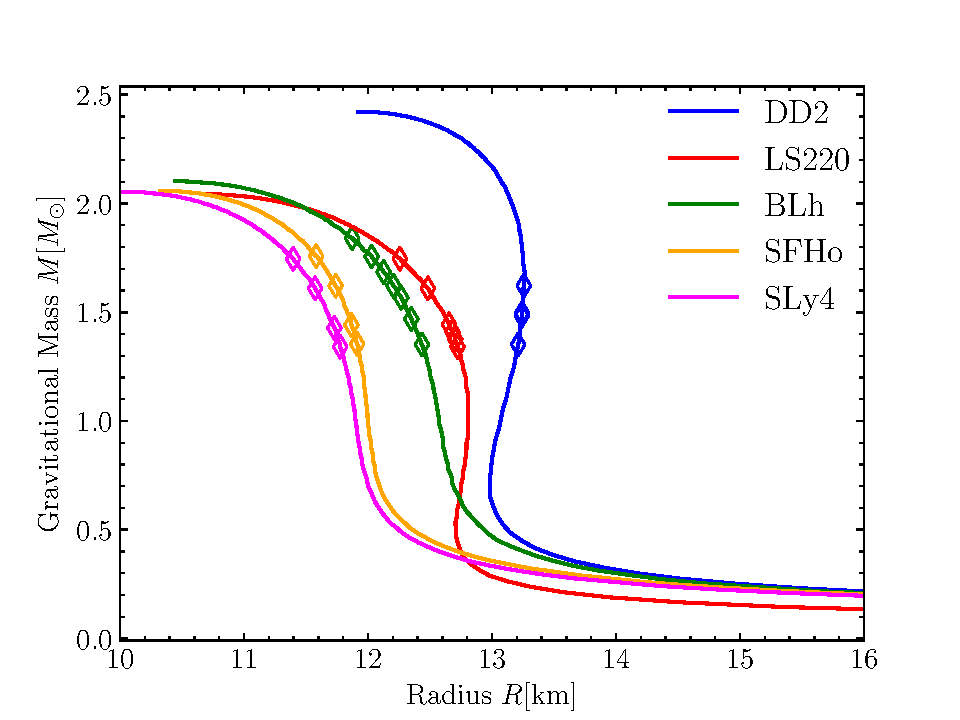
\includegraphics[width=0.49\textwidth]{tov_mr.pdf}
    \caption{Mass-radius relations for the EOSs used in this work. 
        Markers along the sequences indicate the NSs smulated in this work.}  
    \label{fig:method:tov_mr}
\end{figure}

For our models we employ $5$ finite-temperature, composition-dependent equations of state, namely the 
HS(DD2) (hereafter DD2) \cite{Typel:2009sy,Hempel:2009mc}, 
BLh, \cite{Bombaci:2018ksa}, 
LS220, \cite{Lattimer:1991nc}, 
HS(SFHo), (hereafter SFHo) \cite{Steiner:2012rk} and 
SLy4-SOR EOS (hereafter SLy4) \cite{daSilvaSchneider:2017jpg}.

All EOS include neutrinos $(n)$, protons $(p)$, nuclei, electrons, positrons, and photons
as important thermodynamic degrees of freedom.

The radii and maximum masses of neutron stars composed of the cold, neutrino-less $\beta$-equilibrium matter,
from these EOS, fall in line with the current astrophysical constraints, 
\textit{e.g.,} LIGO/Virgo constrain on tidal deformability 
\citep{TheLIGOScientific:2017qsa,Abbott:2018wiz,De:2018uhw,Abbott:2018exr}

All EOS models have symmetry energy at saturation density that are in argeement with experimental limits.
Notably, the LS220 has a especially steep dependency of its symmetry energy on density (\textit{e.g.,} \cite{Lattimer:2012xj,Danielewicz:2013upa}. Thus, this EOS might predict too low symmetry energy below the saturation density. 

%% LS220
The LS220 EOS is based on a non-relativistic (liquid droplet) Skyrme model.
The absolute value of the nuclear bulk incompressibility is set to $220$~MeV, hence, the name.
The EOS includes surface effects and it models $\alpha$-particles as an ideal, classical
non-relativistic gas. For heavy nuclei, the single nucleus approximation is sued. 
%Thus, the the compressible, liquid-drop model with surface effects and composed of ideal gas of 
%particles and heavy nuclei is used to represent the non-homogeneous nuclear matter.
%Heavy nuclei are considered with single nucleus approximation. 
The Gibbs construction is used to model the transition between homogeneous and non-homogeneous matter.
LS220 does not satisfy the constraints from Chiral effective field theory \cite{Hempel:2017ikt}

%% DD2
DD2 (and SFHo) employs the statistical equilibrium to treat the ensemble of several thousands nuclei.
The high-density nuclear matter is treated via RMF approach for unbound nucleons \cite{Hempel:2009mc}.
The excluded volume mechanism is utilized for the phase transition from nuclei to homogeneous
nuclear matter (when densities approch the nuclear saturation density).
DD2 employs the linear, but density dependent coupling for modeling the mean-field nuclear interactions \cite{Typel:2009sy}.
It was however noted that DD2 is not in very good agreement with the so-called flow-constraint \cite{Danielewicz:2002pu}.

%% SFHo [more rephrasing needed!]
Similar to DD2, SFHo combines a statistical ensemble of numerous nuclei, under the assumption of nuclear
statistical equilibrium (NSE) to treat the homogeneous matter, 
with the relativistic mean field approach for the unbound nucleons to treat high-density homogeneous nuclear matter.
It however employs a different parameterizations and values for modeling the mean-field nuclear interactions, 
which is motivated by neutron star radius measurements from low-mass X-ray
binaries (\cite{Steiner:2012rk} and references therein).

The DD2 and SFHo are based on nuclear statistical equilibrium, but 
different parameterizations of the covariant Lagrangian which models the mean-field nuclear interactions.
In these EOSs a finite volume correction coupled to a relativistic mean field theory for treating high-density nuclear matte. However, between these EOSs mean-field nuclear interactions have different parameterizations and values.

%% SLy4
The SLy4 EOS eomplyed in this work is the finite temperature extension \cite{daSilvaSchneider:2017jpg}
of the basic SLY4 Skryme parametrisation for cold nuclear NS matter \cite{Douchin:2001sv}.
The extension includes the non-local isospin asymmetric terms as well as more sophisticated 
treatment of nuclear surface properties and consistent treatment of heavy nuclei size. 
Which is a more advanced version of LS220 treatment (model).
When the phase transition, between the uniform and non-uniform phases, occurs, the phase with lowest 
free energy is chosen, (first order transition).

%% BLh
BLh is a new finite temperature EOS \cite{Logoteta:2020yxf}
This EOS is a finite temperature extension of the cold, $\beta$-equilibrium EOS, \cite{Bombaci:2018ksa},
which was applied to model the BNS merger in \cite{Endrizzi:2018uwl}.
The equation of state is derived in the framework of non-relativistic Brueckner-Hartree-Fock approach.
where microphysical approach based on a specific nuclear interaction is employed for the homogeneous nuclear phase.
The interactions between nucleos are described through a potential derived perturbatively 
in Chiral-Effective-Field theory \cite{Machleidt:2011zz}
The two body interactions are modeled up to second (from the leading term) order, that are used to calculate the local potential. This potential includes $\Delta$-resonances possible excitation. 
Further, the potential is augmented with the three-nucleon force, with the addition of $\Delta$-excitations.
The three-nucleon force was calibrated to reproduce the symmetric nuclear matter at saturatuin density \cite{Logoteta:2016nzc}.
The non-homogeneous phase of the EOS is treated by smoothly connecting the high density BLh EOS to the low-density oart of the SFHo EOS.


\subsubsection{Finite temperature treatment}


Thermal effects are included a different way in these EOS. 
In particular particle correlations beyond the mean field approximation are included only in the BLh EOS.
In other EOS thermal effects enter in the nucleon effective mass, that depend on temperature and density.
These effects, however, are important for the thermal evolution of the NS matter.

%% LS220 and SLy4
In the EOSs that are based on the Skyrme effecrive nuclear interatcions, \textit{e.g.,} LS220 and SLy4
the thermal effects are added in the following form. 
Consider a zero temperature internal energy functional, which depends explicitly on the nuclear density.
The part of this functional that is resposible for interactions is divided into the 
subpart that represents the two-body nucleon-nucleon interactions, (it is quadratic in nuclear density) and a 
subpart that mimics the effect of many body nuclear forces (proportional to the nuclear density in certain power).
Then, both the single particle potentials as well as kinetic energy effective mass dependence play a role
in the temperature dependence of the nuclear effective interaction.
The single particle potential are computed via the variation of the internal energy with respect to the 
neutron and proton densities.
Thus, the smaller the effective masss the larger are kinetic energies and hence, hgiher matter temperature. 
If the entropy remains unchainched.
Thus, the finite temperature behavior of these EOSs is largely set by the nucleon effective mass.
%Then, the smaller the effective mass, the higher the temperature (assuming that entropy is unchanged).
For LS220, the nucleon mass is its bare nucleon mass (for any densities) \gray{so... $m_{N}^*=m_{N}$??}.
For SFHo, $m_N ^* / m_N = 0.76$ at saturation density. 
For DD2 $m_N^*/m_N = 0.56$ 
For BLh $\red{None}$ 
For SLy4 $m_N^*/m_N=0.70$ at saturation density. 
where $m_{N}^*$ is the effective nucleon mass and $m_N$ is the bare nucleon mass.

%% SFHo (and DD2??)
For the SFHo and DD2 EOS, the relativistic Lagrangian considers the $\sigma-$, $\omega-$ and $\rho-$
meson exchanges for descibing nuclear interactions, and the mean-field approximation is used
to solve the resulted Euler-Largrange equations. 
The thermal effects for various species are introduced via Fermi-Dirac distributions at finite temperatures.
Then, self consitent solution of the mean filed eqution introduces the temperature dependence into other 
thermodynamic quantities (through fiurst mesons and nucleon fields)

%% BLh
The BLh EOS employs a different approach to incorporate temperature effects.
The method is based on evaluating the free energy in the Brueckner-Hartree-Fock, which in turn requires,
the effective in-medium nuclear interactions to be defined (starting from the bare nuclear potential).
\gray{This effective interaction is obtained by solving
    the Bethe-Goldstone integral equation which describe the nucleon 
    scattering in the nuclear medium and properly takes into
    account the Pauli principle}.
Then, the nucleon single particle potentials are evaluated (via integration of the on-shell effective interaction matrix)
, which represent the mean field that a nucleon with a certain momenum experience surrounded by other nucleons.
The nucleon single particle potentials, then, allow to evaulate the free energy, and subsequently, 
other thermodynamic quantities.
Notable difference with other EOS discussed here is that the many-body correlations extend beyond the mean field approximation, and are not present in other EOS. 
This EOS was first employed for the BNS merger simulations in \cite{Bernuzzi:2020txg}.

\subsubsection{TOV}

To characterize these EOS, that employs very different microphyscis and finite temperature properties and their relation to the electron fraction, we consider the TOV solutions, presented on the figure \ref{fig:method:tov_mr}.
The maximum mass of a non-rotating NS that these EOSs support are $2.06$, $2.06$, $2.42$ $None$ $None$ 
for SFHo, LS220, DD2, BLh and SLy4 respectively. The NS radii, $R_{1.4}$, then $11.9$, $12.7$, $13.2$ $\red{None}$ $\red{None}$, which in turn is related to the pressure at half saturation density \cite{Lattimer:2012nd}. Thus we adopt the following naming convention for EOS. Those that lead to a NS with smaller radii are called "softer" and those that lead to a NS with larger radii are referred to as "stiffer" EOS.
Among considered, the DD2 is the stiffest EOS, while SLy4 is the softest. 
%% Chapter Template

\chapter{Evolution setup \& post-processing tools} % Main chapter title

\label{Chapter3} % Change X to a consecutive number; for referencing this chapter elsewhere, use \ref{ChapterX}


%% \section{Used codes and setup}
%% \section{Modeling binary neutron star merger with \texttt{WhiskyTHC}}

\section{Initial Data}

For Each EOS considered, we compute the irrotational BNS configurations in quasi-circular orbit.
We employ the pseudo-spectral code \texttt{Lorene} \citep{Gourgoulhon:2000nn}, that 
solves the general relativistic initial data problem.
The initial separation (of the qusi-circular orbit) is chosen $\sim40$~km and that corresponds to $~2-3$ orbits before merger.

The EOS table used for the initial data computation is the minimum temperature slice
$(T\sim 0.5 - 0.1)$~MeV of the finite temperature EOS table used for the evolution.
The assumption of the neutrino-less beta-equilibrium is made.
At constant temperature, at lowest densities, the photon energy (radiation) is a dominant contribution to 
pressure. Thus, we substruct this contribution from the tables.
%Addiitionally, the assuming constant temperature, we also remove the photon (radiation) energy contribution to the pressure (which dominates at the lowest densities)

The EOS table for the minimum temperature slice of the EOS table used for the evolution assuming neutrino-less beta-equilibrium.
Assuming constant temperature, we also remove the photon energy contribution to the pressure.

%In the evolution code, passing the initial data, the mapping is done from the zero temerature
In the evolution code, the electron fraction is set by the beta equilibrium condition. 
The specific internal energy is reset in accordance with minimum temperature slice of the EOS table used for evolution.

Errors present in the initial data in introduced during the mapping result in a small oscillations of netron stars.
In terms of relative changes in central density these amounts to $\sim2-3\%$ \cite{Radice:2018pdn}



\section{Evolution with \texttt{WhiskyTHC}}



In this part we review the numerical relativity code that was used to model binary neutron star mergers analyzed in this thesis.
The part is based on the David Radice PhD thesis where most of the methods are discussed \cite{Radice:2013apa}, and on the published results and regarding code structure and \cite{Radice:2012cu,Radice:2013xpa,Radice:2013hxh,Radice:2015nva}.

In order to perform numerical simulations of fluid flow, accurate numerical codes are essencial. Codes that flux-conservative finite-difference HRSC schemes offer a ciertain degree of simplicity, while high-order finite volume schemes are more computationally expensive (as they require solution of multiple Riemann problems at the interface between regions) \cite{Reisswig:2009us,Shu:2001rep} as well as complex averaging and de-averaging procedures \cite{Tchekhovskoy:2007zn}.

The \texttt{THC} code is the Templated-Hydrodynamics Code developed using the \texttt{Cactus} framework \cite{Goodale:2003}. In \texttt{THC}, the state-of-the-art flux-vector splitting scheme are employed. The "templated" in the code name stands for a modern paradigm in C++ programming, the templated programming, where a part of the code can be generated from the prescribed templates at compiling time (\textit{e.g.,} \cite{Yang:2001})

The \texttt{THC} has several primitive cariable reconstruction schemes implemented, such as MP5, classical monotonicity preserving \cite{Suresh:1997,Mignone:2010} the weighted essentially non oscillatory (WENO) schemes WENO5 and WENO7 \cite{Liu:1994,Jiang:1996,Shu:1997} and two bandwidth-optimized WENO schemes WENO3B and WENO4B \cite{Martin:2006,Taylor:2007}, contracted for modeling the compressible turbulence. Note, that the number in scheme name stands for a formal order of accuracy.

\texttt{WhiskyTHC} is a result of combination of two \texttt{Whisky} \cite{Baiotti:2004wn} and \texttt{THC} \cite{Radice:2012cu}. High-order flux-vector splitting finite-differencing techniques came from the former, while the module for the recovery of the primitive quantities as well as the equation of state framework from the latter \cite{Galeazzi:2013mia}. Tabulated temperature and composition dependent equation of states can be used.

Overall, \texttt{WhiskyTHC} solves the equations of general-relativistic hydrodynamics in conservation form \ref{eq:theory:grhdeq_thc} using a finite difference scheme. \red{tripple check the FD is used for space time evol and central FV method is for hydro}
The flux reconstruction is done in local-characteristic variables using the MP5 scheme, see \textit{e.g.,} \cite{Rezzolla:2013} \red{CHECK}.
The space-time is evolved using the CCZ4 formulation \ref{eq:theory:ccz4equations}, solved via finite difference code publicly available through \texttt{Einstein Toolkit}, \cite{McLachlan,Loffler:2011ay}.\red{CHECK}.
There, the central stencil is used throughout, and only terms associated with the advection along the shift vector are treated using the upwinded by one grid point stencil. The accuracy of the scheme is available at 6th and 8th order, while 4th is commonly employed. In addition, the fifth order Kreiss-Oliger style artificial dissipation \cite{Kreiss:1973} is added to aid with non-linear stability.

The code is build on the \texttt{Carpet} AMR driver \cite{Schnetter:2003rb} from the \texttt{Cactus} computational toolkit \cite{Goodale:2003}, incorporating a provided by \texttt{Carpet} Berger-Oliger-style mesh refinement \cite{Berger:1989,Berger:1984} with subcycling in time and refluxing. \textcolor{red}{in Thesis it is said, -- no refluxing was done yet}

To treat the vacuum region, the code utilizes common, 'atmosphere' approach. The atmosphere is referred to an artificial density floor in the simulation domain. It is introduced in order to tackle the challenges arising when considering boundary between the fluid and vacuum in Eulerian (relativistic) hydrodynamics codes \cite{Galeazzi:mThesis:2008,Kastaun:2006,Millmore:2009dk}. 
The defining property of the atmosphere is that the rest mass density and coordinate velocity are reset to a floor values once the former falls below a certain threshold value during the evolution \cite{Font:2001ew,Baiotti:2004wn}. While showing a reasonable results in second order codes, in higher order ones the numerical oscillations lead to the creation of vacuum nonetheless, that in light of the aforemention atmosphere effect result in the mass and energy violation \cite{Radice:2011qr}. For codes that rely on characteristic variables, the degeneracy in low-density, low-temperature limits also plagues the computation. This problem is the main reason behind the popularity of robust shock capturing codes, even though they are of first order in the general-relativistic hydrodynamics codes. Vacuum treatment for higher order codes is of main challenges to overcome.

There are several approaches in how to treat atmosphere. 

\textit{Standard atmosphere Treatment} or \textit{"ordinary MP5 approach"} is based on setting density that falls below $(1+\epsilon)\rho_{\text{atmo}}$ to the atmosphere density, velocity to zero and internal energy to the one prescubed by the polytropic EoS. The $\rho_{\text{atmo}}$ is usually related to a certain characteristic density, \textit{e.g.,} maximum density at the beginning of the simulation as $\rho_{\text{atmo}} = 10^{-7,-9}\rho_{\text{max}}$. The tolerance parameter $\epsilon$ is usually set to $10^{-2}$ and accounts for excessive oscillations of the fluid–vacuum interface. 

\textit{An Improved Atmosphere Treatment} or \textit{"MP5+LF"} In this approach the component-wise Lax-Friedrichs flux split is turned on when a certain density is reached. This increases the dissipation of the scheme and allows to avoid problems arising in characteristic reconstruction, associated with the degeneracy of the characteristic variables close to vacuum. Unfortunately, if the ejection of low velocity and density matter is concerned, this approach may yield oscillatory solutions and thus creates artifacts. 

\textit{Positivity Preserving Limiter} is an approach discussed in \cite{Radice:2013apa} based on the use of PPL proposed in \cite{Hu:2013}. \gray{Here we provide a brief overview}. \red{No, we not}.
\gray{While for a simplified case of classical gas dynamics it might require a lower timestep, in the general relativistic case and general tabulated EOS, the positivist of pressure is difficult to assure due to complexity of the energy source terms. It can be mitigated by enforcing a floor value on the pressure}. 
Note, that adopting a positivity preserving limiter to treat the transition between matter and vacuum, still implies replacing the vacuum with low density fluid at rest, is not a physically accurate approach. That would rely on treating the transition as a free boundary (see \textit{e.g.,} \cite{Kastaun:2006}) The advantage of positivity preserving limiter with respect to a classical atmosphere treatment, is that it allows to have a value of $\rho_{\text{atmo}}$ that does not require further tuning and can be arbitrary small, and assure that the solution is locally conserved. 
\textcolor{red}{In our models} we employ this approach as follows, at the beginning of the simulations we set the floor density, relying in the subsequent evolution on a positivity preserving limiters to ensure the atmosphere well behavior. Due to negligible density of the atmosphere its accretion has a negligible effect on the evolved object. 

For the extensive tests of different reconstruction methods and atmosphere treatment we refer to the \cite{Radice:2013apa}.


%% \cite{Radice:2012cu,Radice:2013xpa,Radice:2013hxh,Radice:2015nva}


\subsection{Hydrodynamics}



\red{THE IDEA IS THAT YOU PUT MAIN EQ AND THEORY INTO THEORY AND HERE JUST USE THE 'PAPER' STUFF}

The code evolves the proton and neutron number densities, $n_n$ and $n_p$
respectively, as 

\begin{equation}
\label{eq:wthc:pndens}
\nabla_\nu (n_p u^\mu) = R_p^\mu \ \ , \ \ 
\nabla_\nu (n_n u^\mu) = R_n^\mu \ .
\end{equation}

\gray{in Radice2016dwd it is $\nabla_{\alpha}(n_e u^{\alpha}) = R$}

\gray{in Galezzi2013, for Whisky, the equations are separate for baryon and leptons: $\nabla_{\alpha}(n_bu^{\alpha})=0$ and $\nabla_{\alpha}(n_eu^{\alpha})=N$, where the $n_b$ and $n_e$ are the baryon and electron number densities respectively.}

Here $u^{\mu}$ is the fluid four-velocity, $R_p = -R_n$ is the net
lepton number deposition rate due to the absorption and emission of neutrinos 
and antineutrinos (\red{see Section XXX})

The $R_{p,n}$ is computed according to the neutrino M0 scheme \cite{Radice:2016dwd,Radice:2018pdn}

The number densities are related as $n_p=Y_e n$ where $n = n_p + n_e$ is the baryon 
number density and $Y_e$ is electron fraction.

The matter of a neutron star is approximated with ideal fluid with stress-energy tensor

\begin{equation}
T_{\mu\nu} = \rho h u_{\mu} u_{\nu} + Pg_{\mu\nu}
\end{equation}

where $\rho=m_{\text{b}} n$ is the baryon rest-mass density, 
$n$ the baryon number density, $m_{\text{b}} \simeq 10^{-24}\,$g 
the neutron mass, 
\gray{if Galezzi13 it is nucleon mass which is actrually related to the EOS.}
$h=1+\epsilon + P/\rho$ the specific enthalpy, 
$\epsilon$ the specific internal energy (energy density),
and $P$ is \gray{total isotropic} pressure.

Written in a covariant form, the Euler equation for balance of energy and momentum reads

\begin{equation}
\label{eq:wthc:euler}
\nabla_\nu T^{\mu\nu} = Q u^{\mu} \ ,
\end{equation}

\gray{in Radice2016dwd it is $\nabla_{\beta}T^{\alpha\beta}=\Psi^{\alpha}$
    with $\Psi^{\alpha} = Q u^{\alpha}$.
}
\gray{In the Galezzi:2013 it is $\nabla_{\alpha}T^{\alpha\beta}=\Psi^{\beta}$.
    There the $T^{\alpha\beta}$ accounts for the ordinary matter and for trappend neutrinos and photons, but it does not include free-streaming neutrinos. Assumed to be similar to the 'test-fluid' they are neglected in constracting RHS of the Eistein equations.
}

where $Q$ is the net energy deposition rate doe to absorption
and emission of neutrinos also treated with the M0 scheme.
\red{JUST PUT REFS TO THE EQs THAT ARE IN THE 'nuetrino' AND 'viscosity' sections}


\subsection{Numerical methods}


High resolution shock capturing methods are used to discritize equations 
\eqref{eq:wthc:euler} and \eqref{eq:wthc:pndens}.
Specifically, central Kurganov-Tadmor type scheme \cite{Kurganov:2000} with 
HLLE flux formula \cite{Einfeldt:1988}
and non-oscillatory reconstruction of the primitive variables with the MP5 scheme of
\cite{Suresh:1997}.

Shock capturing schemes require the presence of a low density atmosphere around neutron stars.
The constant value of $\rho_0 = m_p n \approx 6\times 10^4$~\gcm.

The rest-mass consirvation in the presence of artificial atmosphere is assured via 
positivity-preserving limiter from \cite{Radice:2013xpa}

The local number densities of neutrons and protons separately, are assured via 
multi-fluid advection method of \cite{Plewa:1998nma}

The outflow properties are extracted when the density exceeds the atmosphere density
by several orders of magnitude.

%% Spacetime evolution
The spacetime is evolved using the Z4c formulation of Einstein's equations
\cite{Bernuzzi:2009ex,Hilditch:2012fp} as implemented in the \texttt{CTGamma} code
\cite{Pollney:2009yz,Reisswig:2013sqa} which is part of the \texttt{Einstein Toolkit} 
\cite{Loffler:2011ay}.

The non-linear stability of evolution is assured via Kreiss-Oliger dissipation. 
The spacial discritisation is done via fourth-order finite-differencing implemented in \texttt{CTGamma}.

The method of lines, MOL, couples the space-time evolution and hydrodynamics. 

Time integrator of choice is strongly-stability preserving third-order Runge-Kutta scheme \cite{Gottlieb:2009}.
The timestep is regulated by the Courant-Friedrichs-Lewy (CFL) condition, that required CFL factor 
to be $<0.25$ for numerical stability. To assure taht the positivity-preserving limiter implemented in \texttt{WhiskyTHC} maintains the density positive, the CFL factor is set to $0.15$.


\subsection{AMR}


The code uses the Berger-Oliger conservative adaptive mesh renement (AMR) \cite{Berger:1984} with 
sub-cycling in time and \red{refluxing (Davids thesis does not have refluxing)} \cite{Berger:1989,Reisswig:2012nc} as provided by the \texttt{Carpet module} of the \texttt{Einstein Toolkit} 
\cite{Schnetter:2003rb}. 


\subsection{Neutrino scheme}


\begin{table}
    \caption{
        Weak reactions employed in our simulations and references for their implementation.
        In the left column, $\nu \in \{\nu_e, \bar{\nu}_e, \nu_{x}\}$ denotes any neutrino species, 
        $\nu_{x}$ any heavy-lepton neutrinos, $N \in\{n, p\}$ a nucleon, and $A$ any nucleus.
        In the central column the role of each reaction is highlighted, with "P" standing for 
        production, "A" for absorption opacity and "S" for scattering opacity. When two roles are
        indicated, the second refers to the inverse ($\leftarrow$) reaction.
        Table is taken from \cite{Radice:2018pdn}.
    }
    \label{tab:leakage}
    \begin{center}
        \begin{tabular}{lll}
            \hline\hline
            Reaction & Role &  Ref. \\ 
            \hline
            $p + e^- \leftrightarrow \nu_e + n $          & P,A & \cite{Bruenn:1985}  \\
            $n + e^+ \leftrightarrow \bar{\nu}_{e} + p $  & P,A & \cite{Bruenn:1985}  \\
            $e^+ + e^- \rightarrow \nu + \bar{\nu}$       & P & \cite{Ruffert:1995fs} \\
            $\gamma + \gamma \rightarrow \nu + \bar{\nu}$ & P & \cite{Ruffert:1995fs} \\
            $N + N \rightarrow \nu + \bar{\nu} + N  + N$  & P & \cite{Burrows:2004vq} \\
            $\nu + N \rightarrow \nu + N$                 & S & \cite{Ruffert:1995fs} \\
            $\nu + A \rightarrow \nu + A$                 & S & \cite{Shapiro:1983du} \\
            \hline\hline
        \end{tabular}
    \end{center}
\end{table}

\red{JUST Name the chemes and reference the equations}
\red{JUST PUT REFS TO THE EQs THAT ARE IN THE 'nuetrino' AND 'viscosity' sections}


\section{General Setup}



The simulation domain is a cube of $3.024$~km each side, whose center is at the center of mass pf the binary.
The AMR structure has $7$ refinemnt levels, with the finest convering both compact objects during the inspiral and the remnant postmerger.

We consider several resolution setups. Low resolution (LR) simulations have $h=246$~m, standard resolution (SR) 
have $h=185$~m and high resolution (HR) $h=123$~m for the final refinemnt level.

In the simulations where the neutirno M0 scheme is included, it is switched on shortly before the merger. 
The equations \eqref{eq:method:whisky:eq7} and \eqref{eq:method:whisky:eq9} are solved on the uniform spherical grid
with radius $\approx 756$~km, and resolution $n_r\times n_{\theta}\times n_{\phi} = 3096 \times 32 \times 64$
grid points.

A subset of models discussed in this thesis include the effective treatment of viscosity. 

We consider \red{$33$} distinct binary with total masses $\red{[None,None]}$ and mass-ratio $q\in[1.00,1.82]$.
In all models the neutrino leackage plus M0 scheme. Most models were computed at at least two resolutions. 
Most our models also include the effect of subgrid turbulence, viscosity.

\gray{Summary of all results in given in the table...}

\gray{Each run is nameed as}

\gray{We simulate each model for at least $\red{None}$~ms after the merger or a few milliseconds after BH formation}



\section{Postprocessing tools and methods}


In order to investigate the neutron star merger dynamics and outflowing material we imploy the following methods and tools.

In order to study and compara on a quantiative level properties of outflow, disk and remnant we employ the mass-averaged quantities and for a quantity $f$ they are computed as 
\begin{equation}
\langle f \rangle = \frac{\sum_i f(m_i)m_i}{\sum_i m_i}
\end{equation}
where $m_i$ is the mass contained in the $i$-th bin.


\subsection{Disk \& Remnant}

It is common to discuss the post-merger state of the binary neutron star systems in terms of the remnant, a neutron star or a black hole, and a disk or torus. However there is not unified convention in how to define the latter and separate it from the former. 

In the case where the remnant is a BH, the disk common disk definition is the matter outside the apparent horizon, (\eg, \cite{Dietrich:2015iva,Dietrich:2016hky}). 
However, owing to the disk accretion onto a black hole, the extraction time is a crutual paramter, and unfortunately is not consistent in the literature, (\eg $\sim1$~ms in \cite{Dietrich:2015iva,Dietrich:2016hky} and $\sim30$~ms in \cite{Sekiguchi:2016bjd}).

In the case where the remnant is a neutron star, the disk definition usually includes the density cut. For instance, in \cite{Radice:2018pdn,Kiuchi:2019lls,Vincent:2019kor} the disk is assumed to encompass the matter with $\rho < 10^{13}$~\gcm. 
The threshold $\rho\sim 10^{13}$~\gcm corresponds to the point in the remnant where
the angular velocity profiles becomes approximately Keplerian, \citep[\eg][]{Shibata:2005ss,Shibata:2006nm,Hanauske:2016gia,Kastaun:2016elu}.
The extraction time here is also important, but less so, as we find that the accretion on the NS is considerably slower.

Overall, we estimate that these differences can amount to a systematic factor of a few,
which we employ for the statistical analysis in section \ref{sec:stat:anal}

% In this thesis we define the disk as a matter that satisfies two criteria $\alpha > 0.15$ and $\tho < 10^{13}\gcm$, where $\alpha$ is the lapse function (see section \ref{sec:theory:gr3p1}).

We compute the baryonic mass of the disks is computed as the volume integral of the conserved rest-mass density $D=\sqrt{\gamma}~W\rho$,

\begin{equation}
\label{eq:method:mdisk}
M_{\text{disk}} = \int D \dd^3 x
\end{equation}

from 3D snapshots of the simulations in postprocessing.



%% In \cite{Sekiguchi:2016bjd}, the disk mass is extracted at
%% ${\approx} 30$~ms outside the AH. In \cite{Radice:2018pdn}, the disk mass is computed
%% as the baryonic mass outside the AH at BH formation, while for NS
%% remnants the criterion $\rho < 10^{13}$ g cm$^{-3}$ is used. 
%% In \cite{Kiuchi:2019lls} for both BH and NS outcome the $\rho < 10^{13}$ g cm$^{-3}$ 
%% criterion is used and time of the extraction is not specified. 
%% In \cite{Vincent:2019kor} the density criterion is the same, however the simulations 
%% are significantly shorter (${~\sim 7.5}$~ms) than in other
%% works. Overall, we estimate that these differences can amount to a
%% systematic factor of a few.



\subsection{Density modes}

%% FROM THE LETTER 

The hydrodynamic instability is monitored by a decomposition in Fourier modes
$e^{-\i m\phi}$ of the Eulerian rest-mass density on the equatorial plane 
[see Eq.~(1) of \citep{Radice:2016gym}] and characterized by the
development of a $m=2$ followed by a $m=1$ mode 
\citep{East:2015vix,Paschalidis:2015mla,Radice:2016gym,Lehner:2016wjg,Bernuzzi:2013rza,Kastaun:2014fna}.
In the short-lived remnant (LS220) the $m=1$ mode
is subdominant with respect to the $m=2$, and it reaches a maximum close to the collapse
\citep{Bernuzzi:2013rza}. Instead, in the long-lived remnant (DD2) the $m=1$
becomes the dominant mode at $\sim$20~ms and persists throughout the
remnant's lifetime, while the $m=2$ efficiently dissipates via
gravitational-wave emission \citep{Bernuzzi:2015opx,Radice:2016gym}.

%% FROM THE PAPER 

During the post-merger evolution the neutron star oscillates. The most prominant modes are quasiradial mode $F$ ($m=0$), the $m=2$ $f$-model and non-linear combinations of them \citep[\eg][]{Shibata:2000jt,Stergioulas:2011gd}.

It has also been shown that the $m=1$, one-armed spiral instability, is present in the remnant of neutron star mergers \citep{Paschalidis:2015mla,Radice:2016gym,East:2016zvv}.

In order to investigate the dynamical instabilities in our simulations we 
project the rest-mass density onto spherical harmonics,
or, in other words, we perform the complex azimuthal mode decomposition of,
the conserved rest-mass density.
For simplicity we consider only $\rho(x,y,z=0,t)$, 
\ie restrict our analysis to the orbital plane $z=0$

\red{DOUBLE check the presence of Gamma and W}
%% \begin{equation}
%% \label{eq:modes}
%% C_m = \int \rho(x,y,z=0,t) W e^{-i m \phi} \sqrt{\gamma} %% \text{d}x \text{d} y \, ,
%% \end{equation}
\begin{equation}
\label{eq:modes}
C_m(t) = \int \rho(x,y,z=0,t) e^{-i m \phi(x,y)} \text{d}x \text{d} y \, ,
\end{equation}
(see \eg~\citet{Baiotti:2009gk}).

% where %% $\rho$ is the rest mass density, 
% $\gamma$ is the determinant of the three-metric and $W$ is the
% Lorentz factor between the fluid and the Eulerian observers. 

Note that the above quantities are gauge dependent.

\red{Dietrich in his thesis thinks that the growing m=1 mode is "We can not
    exclude the possibility that the growing m = 1 mode is triggered by numerical effects,
    but we think that it is a physical hydrodynamical effect due to mode couplings."
    Page 53 of the thesis
}

In addition, friequencies of the modes can be computed with the Fourier analysis of the $\rho_{\text{max}}$ and projections $C_{m}$. We resort it for the future work, as in this work we are interested inly in their magnitude. 





\subsection{Angular momentum}

\red{First, white that in GR the angular momentum is not clearly defined}

%% FROM LETTER 

From the fluid's stress energy tensor,
we compute the angular momentum density flux $J_r = T_{ra}(\partial_\phi)^a$,
where $\phi$ is the cylindrical angular coordinate;
angular momentum is conserved if $(\partial_\phi)^a$ is a Killing vector.

%% FROM PAPER 

The fluid's angular momentum analysis in the remnant and disk is performed
assuming axisymmetry (see Appendix~\ref{app:ang} for derivation).
That is, we assume $\phi^{\mu} = (\partial_{\phi})^{\mu}$ to be a Killing
vector. Accordingly, the conservation law
\begin{equation}
\partial_t(T^{\mu\nu}\phi_{\nu}n_{\nu}\sqrt{\gamma}) -
\partial_i(\alpha T^{i \nu}\phi_{\nu}\sqrt{\gamma}) = 0 \ ,
\end{equation}
where $n^\mu$ is the normal vector to the spacelike hypersurfaces of
the spacetime's $3+1$ decomposition, 
implies the conservation of the angular momentum
\begin{equation}
J = % \int j dV = 
%- \int \, T_{\mu\nu}n^{\mu}\phi^{\nu}\,\dd ^3x = 
-\int \,
T_{\mu\nu}n^{\mu}\phi^{\nu}\,\sqrt{\gamma}\, \dd^3 x\ .
\end{equation}
In the cylindrical coordinates $x^i=(r,\phi,z)$ adapted to the symmetry
the angular momentum density is  
\begin{equation}
j = %-
\rho h W^2 v_{\phi} \ ,
\label{eq:method:ang_mom}
\end{equation}
and the angular momentum flux is 
\begin{equation}
\alpha\sqrt{\gamma}T^r _{\nu}\phi^{\nu} =
\alpha\sqrt{\gamma}\rho h W^2 (v^{r}v_{\phi}) .
\end{equation}


\subsection{Ejecta}


To model and study the electromagnetic counterparts to mergers, the amount and properties of the material
leaving the system are needed.
The matter expelled at high velocity may ultimately become unbound from the central gravitational
potential. There are two indicators commonly adopted to mark the unbound matter.

\subsubsection{The Geodesic criterion}

Assuming that the spacetime is stationary, the $\partial_t$ is the killing vectory \red{confirm}, 
the four-velocity, $u_t$, (along the time-like killing vector), is a constant of motion for geodesics. 
Additionally, if the space is asymptotically flat, at infinity the $u_t = -W$, where $W$ is the fluid element Lorentz factor. Then, if a fluid element has $u_t < -1$, it may be considered unbound \red{as it will retain the non-zero positive velocity at infinity}. 
The fluid reaches an asymptotic velocity 
\begin{equation}
\upsilon_{\infty} \simeq \sqrt{2E_{\infty}} = \sqrt{(1-u_t ^2)}.
\end{equation}
The criterion can be through of as considering the fluid to be made of isolated particles that follow the geodesics. Indeed, the effects of equation of state, fluids pressure gradient, internal energy and heating (\eg, due to an $r$-process (\red{see section XXX})) are neglected. The space time is also assumed to be static.
Strictly speaking, none of these assumptions is fulfilled in the BNS post-merger environment. However, this criterion is widely used in the literature \citep[\eg][]{Radice:2018pdn,Vincent:2019kor}.
Note that the geodesic criterion above neglects the fluid's pressure and might underestimate the ejecta mass.

\subsubsection{The Bernoulli criterion}

From the relativistic Bernoulli equation \citep{Rezzolla:2013}, it follows
that for a stationary relativisitc flow, the $hu_t$ is constnat along the 
fluid worldliens. Here $h$ is the (relativistic) enthalpy, which is
defined up to a constant factor. 
If at the spatial infinity the enthalpy is set so $h\rightarrow-1$, 
\red{in Vincent it is $h\leftarrow 1$}
the condition $hu_t < -1$ would mark the unbound matter 
(as in the assymptotically flat space-time the $u_t = -W$ for the flow particles following geodesics).

The associated asymptotic velocity is calculated as 
\begin{equation}
\upsilon_{\infty} \simeq \sqrt{2 (h (E_{\infty}+1)-1)}. 
\end{equation}

The criterion can be regarded as assuming all the internal energy of the fluid 
gets added to the fluid kinetic energy, as the fluid decompresses \red{(pressure drops?)}.

The $r$-process nucleosynthesis that occurs in the outflow deposits the energy.
\red{In Vincent it is assumed that the difference in binding energy between the 
    particles in NSE at a given $\rho$, $T$ and $Y_e$, and their binding energy at
    the same $Y_e$ but low $\rho$ and $T$ is added/substracted from the fluid's kinetic energy.
    Out-of-NSE evolution and effects this neglected \citep[][see]{Foucart:2016vxd}
    [BUT I AM NOT SURE IF THIS IS THE CASE FOR OUR SIMULATIONS! MAYBE NOT!]}

This criterion has been found to estimate more accurately the amount of unbound material \citep{Foucart:2015gaa}
However, as was also found that the Bernoulli criterion leads to up to twice the amount of ejecta detected in comparion with the geodensic criterion, if the estimation is done within a given volume \citep{Kastaun:2014fna}.

We adopt the geodesic criterion to study the "burst-like", short outflows,
such as dynamical ejecta, where the pressure gradient is not expected to make a significant contribution.
For the steady-state outflows, like postmerger winds we adopt the Bernoulli criterion.

The term ejecta would refer to the material gravitationaly unbound according to eather of the criteria.




All considered mass ejecta are calculated on a coordinate sphere at $R \simeq 294$km. 
\red{untill afterglow}

 
% Chapter Template

\chapter{Results and discussions} % Main chapter title

\label{Chapter4} % Change X to a consecutive number; for referencing this chapter elsewhere, use \ref{ChapterX}

%----------------------------------------------------------------------------------------
%	SECTION 1
%----------------------------------------------------------------------------------------

\red{
    To be defined: \\
    Chirp pass \\
    Gravitational and Baryonic masses
}

In this chapter we review the findings of \citet{Nedora:2019jhl} and \citet{Nedora:2020pak}
and investigate the long-term \pmerg{} evolution of the binary neutron star. 

Such studies are of high astrophysical importance as the ejecta of matter that occur 
on various timescales \pmerg{} undergoes \rproc{} and produces observable EM emission. 
The discussion of the \rproc{} and EM transits themselves, we resort for the chapter \red{chap:coutnerparts}.


\section{Simulations}



%% --------------------------------
%% TAB SIM SUMMARY
%\begin{table*}
\begin{sidewaystable}
\begin{center}
\captionsetup{width=1.0\linewidth}
    \caption{
      Summary table of all the simulations and dynamical ejecta properties. The columns contain
      the following information, starting from the left. Equation of
      state, mass-ratio, available resolutions,
      inclusion of subgrid turbulence, time of the
      simulation end, time of the BH formation for LR, SR, HR
      resolutions separately, time of last output, time the disk mass
      is extracted, disk mass, mass of the
      dynamical ejecta, mass-averaged electron fracton, terminal
      velocity and RMS angle (from the binary plane) for dynamical ejecta. For all
      data except $t_{BH}$, $t_{\text{end}}$ and $t_{\text{disk}}$, the value that is given is a mean value across resolutions, with an error estimated as one
      standard diviaion from the mean. In case where only one
      resolution is present, the error is assumed to be $20\%$ of the
      value. Adopted from \citet{Nedora:2020pak}.
    }
      %% \newtxt{For discussions on errors and convergence see \citep{Radice:2018pdn,Bernuzzi:2020txg}.
      %% The model data are available online at \citep{vsevolod_nedora_2020_4159619}.
%%       }
\scalebox{0.70}{
\begin{tabular}{c c c c c c c c c c c c c}
    \hline\hline
    EOS & $q$ & $\tilde{\Lambda}$ & Resolution & GRLES & $t_{\text{end}}$ & $t_{\text{BH}}$ & $t_{\text{disk}}$ & $M_{\text{disk}} ^{\text{last}}$ & $\md$ & $\langle \yd \rangle$ & $\langle \vd  \rangle$ & $\langle \theta_{\text{ej}} ^{\text{d}} \rangle$ \\
    &   &   &  &  & [ms] & [ms] & [ms] &   & $[10^{-2} M_{\odot}]$ &   & $[c]$ &   \\ 
    \hline
    \hline
    BLh & 1.00 & 541 & \texttt{LR SR HR} & \cmark & $43.3$ $91.8$ $23.1$ & $>43.3$ $>91.8$ $>23.1$ & 23.1 & $0.166^{+0.052} _{-0.052} $ & $0.14^{+0.02} _{-0.02} $ & $0.27^{+0.01} _{-0.01} $ & $0.17^{+0.01} _{-0.01} $ & $39.65^{+0.35} _{-0.35} $ \\
    BLh & 1.00 & 541 & \texttt{LR SR} & \xmark & $15.9$ $103.2$ $ $ & $>15.9$ $>103.2$ $ $ & 15.6 & $0.261^{+0.008} _{-0.008} $ & $0.12^{+0.01} _{-0.01} $ & $0.27^{+0.01} _{-0.01} $ & $0.16^{+0.01} _{-0.01} $ & $38.80^{+0.44} _{-0.44} $ \\
%%  BLh & 1.00 & 541 & \texttt{LR SR} & \xmark & $36.9$ $15.5$ $ $ & $>36.9$ $>15.5$ $ $ & 36.6 & $0.182^{+0.091} _{-0.091} $ & $0.21^{+0.04} _{-0.04} $ & $0.26^{+0.01} _{-0.01} $ & $0.18^{+0.01} _{-0.01} $ & $36.29^{+0.24} _{-0.24} $ \\
    \hline
    BLh & 1.18 & 539 & \texttt{LR} & \cmark & $69.4$ $ $ $ $ & $>69.4$ $ $ $ $ & 69.0 & $0.202^{+0.101} _{-0.101} $ & $0.30^{+0.06} _{-0.06} $ & $0.18^{+0.04} _{-0.04} $ & $0.19^{+0.04} _{-0.04} $ & $33.65^{+6.73} _{-6.73} $ \\
    BLh & 1.18 & 539 & \texttt{LR} & \xmark & $16.4$ $ $ $ $ & $>16.4$ $ $ $ $ & 15.9 & $0.229^{+0.115} _{-0.115} $ & $0.25^{+0.05} _{-0.05} $ & $0.16^{+0.03} _{-0.03} $ & $0.20^{+0.04} _{-0.04} $ & $30.86^{+6.17} _{-6.17} $ \\
    \hline
    BLh & 1.34 & 539 & \texttt{LR SR} & \cmark & $63.4$ $9.8$ $ $ & $>63.4$ $>9.8$ $ $ & 9.8 & $0.192^{+0.004} _{-0.004} $ & $0.25^{+0.05} _{-0.05} $ & $0.14^{+0.04} _{-0.04} $ & $0.17^{+0.00} _{-0.00} $ & $28.79^{+5.00} _{-5.00} $ \\
    BLh & 1.34 & 539 & \texttt{LR} & \xmark & $18.0$ $ $ $ $ & $>18.0$ $ $ $ $ & 18.0 & $0.211^{+0.106} _{-0.106} $ & $0.19^{+0.04} _{-0.04} $ & $0.17^{+0.03} _{-0.03} $ & $0.17^{+0.03} _{-0.03} $ & $33.39^{+6.68} _{-6.68} $ \\
    \hline
    BLh & 1.43 & 540 & \texttt{LR SR} & \cmark & $35.1$ $59.6$ $ $ & $>35.1$ $>59.6$ $ $ & 33.8 & $0.265^{+0.001} _{-0.001} $ & $0.27^{+0.08} _{-0.08} $ & $0.19^{+0.03} _{-0.03} $ & $0.16^{+0.00} _{-0.00} $ & $34.49^{+3.59} _{-3.59} $ \\
    \hline
    BLh & 1.54 & 543 & \texttt{LR} & \cmark & $45.8$ $ $ $ $ & $>45.8$ $ $ $ $ & 53.8 & $0.324^{+0.162} _{-0.162} $ & $0.20^{+0.04} _{-0.04} $ & $0.17^{+0.03} _{-0.03} $ & $0.13^{+0.03} _{-0.03} $ & $31.21^{+6.24} _{-6.24} $ \\
    BLh & 1.54 & 543 & \texttt{LR} & \xmark & $17.4$ $ $ $ $ & $>17.4$ $ $ $ $ & 30.1 & $0.287^{+0.144} _{-0.144} $ & $0.22^{+0.04} _{-0.04} $ & $0.21^{+0.04} _{-0.04} $ & $0.16^{+0.03} _{-0.03} $ & $35.05^{+7.01} _{-7.01} $ \\
    \hline
    BLh & 1.66 & 538 & \texttt{LR SR} & \cmark & $64.6$ $20.1$ $ $ & $>64.6$ $1.8$ $ $ & 19.2 & $0.289^{+0.005} _{-0.005} $ & $0.42^{+0.05} _{-0.05} $ & $0.11^{+0.01} _{-0.01} $ & $0.12^{+0.01} _{-0.01} $ & $24.08^{+0.29} _{-0.29} $ \\
    \hline
    BLh & 1.82 & 532 & \texttt{LR SR HR} & \cmark & $12.0$ $17.5$ $9.6$ & $1.4$ $1.4$ $1.5$ & 5.9 & $0.170^{+0.001} _{-0.001} $ & $0.81^{+0.04} _{-0.04} $ & $0.03^{+0.01} _{-0.01} $ & $0.11^{+0.00} _{-0.00} $ & $6.53^{+0.65} _{-0.65} $ \\
    BLh & 1.82 & 532 & \texttt{LR SR HR} & \xmark & $53.8$ $26.3$ $45.2$ & $1.7$ $1.3$ $1.0$ & 43.2 & $0.098^{+0.049} _{-0.049} $ & $1.07^{+0.07} _{-0.07} $ & $0.03^{+0.01} _{-0.01} $ & $0.12^{+0.00} _{-0.00} $ & $6.27^{+0.53} _{-0.53} $ \\
    \hline
    \hline
    DD2 & 1.00 & 853 & \texttt{LR SR}    & \xmark & $92.0$ $110.2$       & $>92.0$ $>110.2$        & 9.4 & $0.154^{+0.052} _{-0.052} $ & $0.11^{+0.01} _{-0.01} $ & $0.25^{+0.00} _{-0.00} $ & $0.18^{+0.01} _{-0.01} $ & $38.07^{+0.52} _{-0.52} $ \\
    DD2 & 1.00 & 853 & \texttt{LR SR HR} & \cmark & $123.0$ $113.0$ $74.4$ & $>123.0$ $>113.0$ $>74.4$ & 8.2 & $0.111^{+0.040} _{-0.040} $ & $0.12^{+0.03} _{-0.03} $ & $0.27^{+0.01} _{-0.01} $ & $0.16^{+0.00} _{-0.00} $ & $40.03^{+0.71} _{-0.71} $ \\
    \hline
    DD2 & 1.20 & 847 & \texttt{LR SR HR} & \xmark & $37.3$ $91.0$ $55.2$ & $>37.3$ $>91.0$ $>55.2$ & 36.6 & $0.261^{+0.028} _{-0.028} $ & $0.21^{+0.08} _{-0.08} $ & $0.18^{+0.03} _{-0.03} $ & $0.17^{+0.01} _{-0.01} $ & $29.07^{+3.75} _{-3.75} $ \\
    DD2 & 1.22 & 847 & \texttt{LR SR HR} & \cmark & $42.7$ $107.3$ $19.8$ & $>42.7$ $>107.3$ $>19.8$ & 8.7 & $0.209^{+0.033} _{-0.033} $ & $0.25^{+0.02} _{-0.02} $ & $0.19^{+0.01} _{-0.01} $ & $0.17^{+0.01} _{-0.01} $ & $30.74^{+0.89} _{-0.89} $ \\
    \hline
    DD2 & 1.43 & 820 & \texttt{LR SR} & \cmark & $37.7$ $62.0$ $ $ & $>37.7$ $>62.0$ $ $ & 36.7 & $0.304^{+0.051} _{-0.051} $ & $0.70^{+0.64} _{-0.64} $ & $0.14^{+0.05} _{-0.05} $ & $0.14^{+0.01} _{-0.01} $ & $25.51^{+9.58} _{-9.58} $ \\
    \hline
    \hline
    LS220 & 1.00 & 715 & \texttt{LR SR} & \cmark & $27.0$ $27.1$ $ $ & $13.7$ $13.7$ $ $ & 16.1 & $0.073^{+0.032} _{-0.032} $ & $0.16^{+0.02} _{-0.02} $ & $0.25^{+0.02} _{-0.02} $ & $0.16^{+0.01} _{-0.01} $ & $35.70^{+0.78} _{-0.78} $ \\
    LS220 & 1.00 & 715 & \texttt{LR SR HR} & \xmark & $35.9$ $37.2$ $27.1$ & $33.4$ $16.1$ $15.4$ & 34.6 & $0.072^{+0.006} _{-0.006} $ & $0.16^{+0.06} _{-0.06} $ & $0.22^{+0.00} _{-0.00} $ & $0.16^{+0.01} _{-0.01} $ & $34.99^{+1.68} _{-1.68} $ \\
    \hline
    LS220 & 1.05 & 715 & \texttt{SR HR} & \xmark & $ $ $23.3$ $24.1$ & $ $ $17.3$ $13.9$ & 22.3 & $0.107^{+0.054} _{-0.054} $ & $0.16^{+0.02} _{-0.02} $ & $0.21^{+0.01} _{-0.01} $ & $0.16^{+0.01} _{-0.01} $ & $33.28^{+2.37} _{-2.37} $ \\
    LS220 & 1.11 & 717 & \texttt{SR HR} & \xmark & $ $ $25.1$ $24.4$ & $ $ $17.0$ $>24.4$ & 24.2 & $0.140^{+0.071} _{-0.071} $ & $0.22^{+0.03} _{-0.03} $ & $0.19^{+0.02} _{-0.02} $ & $0.18^{+0.02} _{-0.02} $ & $30.25^{+4.43} _{-4.43} $ \\
    \hline
    LS220 & 1.16 & 714 & \texttt{SR HR} & \cmark & $ $ $95.8$ $11.3$ & $ $ $68.9$ $>11.3$ & 95.5 & $0.306^{+0.153} _{-0.153} $ & $0.34^{+0.00} _{-0.00} $ & $0.22^{+0.00} _{-0.00} $ & $0.16^{+0.00} _{-0.00} $ & $34.08^{+1.00} _{-1.00} $ \\
    LS220 & 1.16 & 714 & \texttt{LR SR HR} & \xmark & $29.5$ $36.1$ $28.8$ & $>29.5$ $>36.1$ $24.1$ & - & - & $0.33^{+0.05} _{-0.05} $ & $0.17^{+0.01} _{-0.01} $ & $0.17^{+0.01} _{-0.01} $ & $30.01^{+0.64} _{-0.64} $ \\
    \hline
    LS220 & 1.43 & 710 & \texttt{LR SR} & \cmark & $19.8$ $28.5$ $ $ & $15.7$ $12.3$ $ $ & 19.6 & $0.178^{+0.072} _{-0.072} $ & $0.73^{+0.03} _{-0.03} $ & $0.16^{+0.02} _{-0.02} $ & $0.17^{+0.01} _{-0.01} $ & $26.77^{+3.50} _{-3.50} $ \\
    \hline
    LS220 & 1.66 & 707 & \texttt{LR SR} & \cmark & $6.8$ $8.0$ $ $ & $1.4$ $2.1$ $ $ & 2.0 & $0.068^{+0.008} _{-0.008} $ & $1.11^{+0.38} _{-0.38} $ & $0.07^{+0.01} _{-0.01} $ & $0.14^{+0.01} _{-0.01} $ & $13.18^{+1.33} _{-1.33} $ \\
    \hline
    \hline
    SFHo & 1.00 & 413 & \texttt{SR HR} & \cmark & $ $ $25.3$ $11.6$ & $ $ $6.0$ $4.0$ & 50.0 & $0.023^{+0.012} _{-0.012} $ & $0.40^{+0.07} _{-0.07} $ & $0.21^{+0.00} _{-0.00} $ & $0.19^{+0.01} _{-0.01} $ & $32.48^{+1.79} _{-1.79} $ \\
    SFHo & 1.00 & 413 & \texttt{LR SR HR} & \xmark & $3.2$ $7.7$ $9.0$ & $>3.2$ $4.1$ $3.8$ & 7.2 & $0.019^{+0.007} _{-0.007} $ & $0.28^{+0.07} _{-0.07} $ & $0.23^{+0.01} _{-0.01} $ & $0.21^{+0.01} _{-0.01} $ & $31.66^{+1.80} _{-1.80} $ \\
    \hline
    SFHo & 1.13 & 412 & \texttt{SR HR} & \cmark & $ $ $14.2$ $14.3$ & $ $ $6.3$ $>14.3$ & - & - & $0.44^{+0.12} _{-0.12} $ & $0.18^{+0.01} _{-0.01} $ & $0.23^{+0.01} _{-0.01} $ & $33.20^{+0.78} _{-0.78} $ \\
    SFHo & 1.13 & 412 & \texttt{LR SR HR} & \xmark & $16.5$ $19.3$ $15.2$ & $5.5$ $11.6$ $3.9$ & 15.1 & $0.046^{+0.041} _{-0.041} $ & $0.42^{+0.03} _{-0.03} $ & $0.17^{+0.03} _{-0.03} $ & $0.22^{+0.01} _{-0.01} $ & $29.63^{+4.39} _{-4.39} $ \\
    \hline
    SFHo & 1.43 & 414 & \texttt{LR} & \cmark & $19.6$ $ $ $ $ & $4.8$ $ $ $ $ & 18.9 & $0.201^{+0.101} _{-0.101} $ & $0.38^{+0.08} _{-0.08} $ & $0.14^{+0.03} _{-0.03} $ & $0.20^{+0.04} _{-0.04} $ & $29.20^{+5.84} _{-5.84} $ \\
    SFHo & 1.43 & 414 & \texttt{SR} & \cmark & $ $ $46.5$ $ $ & $ $ $>46.5$ $ $ & 50.8 & $0.241^{+0.121} _{-0.121} $ & $0.24^{+0.05} _{-0.05} $ & $0.19^{+0.04} _{-0.04} $ & $0.14^{+0.03} _{-0.03} $ & $32.86^{+6.57} _{-6.57} $ \\
    \hline
    SFHo & 1.66 & 408 & \texttt{LR SR} & \cmark & $11.2$ $16.8$ $ $ & $1.3$ $1.3$ $ $ & 11.6 & $0.177^{+0.153} _{-0.153} $ & $0.15^{+0.00} _{-0.00} $ & $0.07^{+0.00} _{-0.00} $ & $0.12^{+0.01} _{-0.01} $ & $10.39^{+1.14} _{-1.14} $ \\
    \hline
    \hline
    SLy4 & 1.00 & 402 & \texttt{LR SR} & \cmark & $10.5$ $13.1$ $ $ & $2.8$ $2.8$ $ $ & - & - & $0.09^{+0.02} _{-0.02} $ & $0.23^{+0.02} _{-0.02} $ & $0.27^{+0.02} _{-0.02} $ & $30.81^{+2.81} _{-2.81} $ \\
    SLy4 & 1.00 & 402 & \texttt{LR SR} & \xmark & $12.7$ $22.0$ $ $ & $2.7$ $13.8$ $ $ & 12.5 & $0.071^{+0.175} _{-0.175} $ & $0.31^{+0.20} _{-0.20} $ & $0.23^{+0.03} _{-0.03} $ & $0.22^{+0.01} _{-0.01} $ & $32.23^{+4.84} _{-4.84} $ \\
    \hline
    SLy4 & 1.13 & 402 & \texttt{LR SR} & \xmark & $8.4$ $20.3$ $ $ & $>8.4$ $13.0$ $ $ & 8.0 & $0.164^{+0.023} _{-0.023} $ & $0.59^{+0.07} _{-0.07} $ & $0.16^{+0.00} _{-0.00} $ & $0.24^{+0.01} _{-0.01} $ & $29.67^{+1.97} _{-1.97} $ \\
    \hline
    SLy4 & 1.43 & 399 & \texttt{SR} & \cmark & $ $ $40.3$ $ $ & $ $ $>40.3$ $ $ & 45.2 & $0.200^{+0.100} _{-0.100} $ & $0.20^{+0.04} _{-0.04} $ & $0.21^{+0.04} _{-0.04} $ & $0.15^{+0.03} _{-0.03} $ & $34.03^{+6.81} _{-6.81} $ \\
    \hline
    SLy4 & 1.66 & 397 & \texttt{SR} & \cmark & $ $ $7.2$ $ $ & $ $ $1.2$ $ $ & 3.9 & $0.138^{+0.069} _{-0.069} $ & $0.28^{+0.06} _{-0.06} $ & $0.05^{+0.01} _{-0.01} $ & $0.12^{+0.02} _{-0.02} $ & $8.43^{+1.69} _{-1.69} $ \\
    \hline\hline
\end{tabular}
\label{tab:sim}
}%scalebox
\end{center}
%\end{table*}
\end{sidewaystable}



%\usepackage{lipsum}% dummy text
%\begin{document}
    %\lipsum % Text before
%    \afterpage{%
%        \clearpage% Flush earlier floats (otherwise order might not be correct)
%        \thispagestyle{empty}% empty page style (?)
%        \begin{landscape}% Landscape page
%            \centering % Center table
%            \begin{tabular}{c c c c c c c c c c c c c}
%                \hline\hline
%                EOS & $q$ & $\tilde{\Lambda}$ & Resolution & GRLES & $t_{\text{end}}$ & $t_{\text{BH}}$ & $t_{\text{disk}}$ & $M_{\text{disk}} ^{\text{last}}$ & $\md$ & $\langle \yd \rangle$ & $\langle \vd  \rangle$ & $\langle \theta_{\text{ej}} ^{\text{d}} \rangle$ \\
%                &   &   &  &  & [ms] & [ms] & [ms] &   & $[10^{-2} M_{\odot}]$ &   & $[c]$ &   \\ 
%                \hline
%                \hline
%                BLh & 1.00 & 541 & \texttt{LR SR HR} & \cmark & $43.3$ $91.8$ $23.1$ & $>43.3$ $>91.8$ $>23.1$ & 23.1 & $0.166^{+0.052} _{-0.052} $ & $0.14^{+0.02} _{-0.02} $ & $0.27^{+0.01} _{-0.01} $ & $0.17^{+0.01} _{-0.01} $ & $39.65^{+0.35} _{-0.35} $ \\
%                BLh & 1.00 & 541 & \texttt{LR SR} & \xmark & $15.9$ $103.2$ $ $ & $>15.9$ $>103.2$ $ $ & 15.6 & $0.261^{+0.008} _{-0.008} $ & $0.12^{+0.01} _{-0.01} $ & $0.27^{+0.01} _{-0.01} $ & $0.16^{+0.01} _{-0.01} $ & $38.80^{+0.44} _{-0.44} $ \\
%                %%  BLh & 1.00 & 541 & \texttt{LR SR} & \xmark & $36.9$ $15.5$ $ $ & $>36.9$ $>15.5$ $ $ & 36.6 & $0.182^{+0.091} _{-0.091} $ & $0.21^{+0.04} _{-0.04} $ & $0.26^{+0.01} _{-0.01} $ & $0.18^{+0.01} _{-0.01} $ & $36.29^{+0.24} _{-0.24} $ \\
%                \hline
%                BLh & 1.18 & 539 & \texttt{LR} & \cmark & $69.4$ $ $ $ $ & $>69.4$ $ $ $ $ & 69.0 & $0.202^{+0.101} _{-0.101} $ & $0.30^{+0.06} _{-0.06} $ & $0.18^{+0.04} _{-0.04} $ & $0.19^{+0.04} _{-0.04} $ & $33.65^{+6.73} _{-6.73} $ \\
%                BLh & 1.18 & 539 & \texttt{LR} & \xmark & $16.4$ $ $ $ $ & $>16.4$ $ $ $ $ & 15.9 & $0.229^{+0.115} _{-0.115} $ & $0.25^{+0.05} _{-0.05} $ & $0.16^{+0.03} _{-0.03} $ & $0.20^{+0.04} _{-0.04} $ & $30.86^{+6.17} _{-6.17} $ \\
%                \hline
%                BLh & 1.34 & 539 & \texttt{LR SR} & \cmark & $63.4$ $9.8$ $ $ & $>63.4$ $>9.8$ $ $ & 9.8 & $0.192^{+0.004} _{-0.004} $ & $0.25^{+0.05} _{-0.05} $ & $0.14^{+0.04} _{-0.04} $ & $0.17^{+0.00} _{-0.00} $ & $28.79^{+5.00} _{-5.00} $ \\
%                BLh & 1.34 & 539 & \texttt{LR} & \xmark & $18.0$ $ $ $ $ & $>18.0$ $ $ $ $ & 18.0 & $0.211^{+0.106} _{-0.106} $ & $0.19^{+0.04} _{-0.04} $ & $0.17^{+0.03} _{-0.03} $ & $0.17^{+0.03} _{-0.03} $ & $33.39^{+6.68} _{-6.68} $ \\
%                \hline
%                BLh & 1.43 & 540 & \texttt{LR SR} & \cmark & $35.1$ $59.6$ $ $ & $>35.1$ $>59.6$ $ $ & 33.8 & $0.265^{+0.001} _{-0.001} $ & $0.27^{+0.08} _{-0.08} $ & $0.19^{+0.03} _{-0.03} $ & $0.16^{+0.00} _{-0.00} $ & $34.49^{+3.59} _{-3.59} $ \\
%                \hline
%                BLh & 1.54 & 543 & \texttt{LR} & \cmark & $45.8$ $ $ $ $ & $>45.8$ $ $ $ $ & 53.8 & $0.324^{+0.162} _{-0.162} $ & $0.20^{+0.04} _{-0.04} $ & $0.17^{+0.03} _{-0.03} $ & $0.13^{+0.03} _{-0.03} $ & $31.21^{+6.24} _{-6.24} $ \\
%                BLh & 1.54 & 543 & \texttt{LR} & \xmark & $17.4$ $ $ $ $ & $>17.4$ $ $ $ $ & 30.1 & $0.287^{+0.144} _{-0.144} $ & $0.22^{+0.04} _{-0.04} $ & $0.21^{+0.04} _{-0.04} $ & $0.16^{+0.03} _{-0.03} $ & $35.05^{+7.01} _{-7.01} $ \\
%                \hline
%                BLh & 1.66 & 538 & \texttt{LR SR} & \cmark & $64.6$ $20.1$ $ $ & $>64.6$ $1.8$ $ $ & 19.2 & $0.289^{+0.005} _{-0.005} $ & $0.42^{+0.05} _{-0.05} $ & $0.11^{+0.01} _{-0.01} $ & $0.12^{+0.01} _{-0.01} $ & $24.08^{+0.29} _{-0.29} $ \\
%                \hline
%                BLh & 1.82 & 532 & \texttt{LR SR HR} & \cmark & $12.0$ $17.5$ $9.6$ & $1.4$ $1.4$ $1.5$ & 5.9 & $0.170^{+0.001} _{-0.001} $ & $0.81^{+0.04} _{-0.04} $ & $0.03^{+0.01} _{-0.01} $ & $0.11^{+0.00} _{-0.00} $ & $6.53^{+0.65} _{-0.65} $ \\
%                BLh & 1.82 & 532 & \texttt{LR SR HR} & \xmark & $53.8$ $26.3$ $45.2$ & $1.7$ $1.3$ $1.0$ & 43.2 & $0.098^{+0.049} _{-0.049} $ & $1.07^{+0.07} _{-0.07} $ & $0.03^{+0.01} _{-0.01} $ & $0.12^{+0.00} _{-0.00} $ & $6.27^{+0.53} _{-0.53} $ \\
%                \hline
%                \hline
%                DD2 & 1.00 & 853 & \texttt{LR SR}    & \xmark & $92.0$ $110.2$       & $>92.0$ $>110.2$        & 9.4 & $0.154^{+0.052} _{-0.052} $ & $0.11^{+0.01} _{-0.01} $ & $0.25^{+0.00} _{-0.00} $ & $0.18^{+0.01} _{-0.01} $ & $38.07^{+0.52} _{-0.52} $ \\
%                DD2 & 1.00 & 853 & \texttt{LR SR HR} & \cmark & $123.0$ $113.0$ $74.4$ & $>123.0$ $>113.0$ $>74.4$ & 8.2 & $0.111^{+0.040} _{-0.040} $ & $0.12^{+0.03} _{-0.03} $ & $0.27^{+0.01} _{-0.01} $ & $0.16^{+0.00} _{-0.00} $ & $40.03^{+0.71} _{-0.71} $ \\
%                \hline
%                DD2 & 1.20 & 847 & \texttt{LR SR HR} & \xmark & $37.3$ $91.0$ $55.2$ & $>37.3$ $>91.0$ $>55.2$ & 36.6 & $0.261^{+0.028} _{-0.028} $ & $0.21^{+0.08} _{-0.08} $ & $0.18^{+0.03} _{-0.03} $ & $0.17^{+0.01} _{-0.01} $ & $29.07^{+3.75} _{-3.75} $ \\
%                DD2 & 1.22 & 847 & \texttt{LR SR HR} & \cmark & $42.7$ $107.3$ $19.8$ & $>42.7$ $>107.3$ $>19.8$ & 8.7 & $0.209^{+0.033} _{-0.033} $ & $0.25^{+0.02} _{-0.02} $ & $0.19^{+0.01} _{-0.01} $ & $0.17^{+0.01} _{-0.01} $ & $30.74^{+0.89} _{-0.89} $ \\
%                \hline
%                DD2 & 1.43 & 820 & \texttt{LR SR} & \cmark & $37.7$ $62.0$ $ $ & $>37.7$ $>62.0$ $ $ & 36.7 & $0.304^{+0.051} _{-0.051} $ & $0.70^{+0.64} _{-0.64} $ & $0.14^{+0.05} _{-0.05} $ & $0.14^{+0.01} _{-0.01} $ & $25.51^{+9.58} _{-9.58} $ \\
%                \hline
%                \hline
%                LS220 & 1.00 & 715 & \texttt{LR SR} & \cmark & $27.0$ $27.1$ $ $ & $13.7$ $13.7$ $ $ & 16.1 & $0.073^{+0.032} _{-0.032} $ & $0.16^{+0.02} _{-0.02} $ & $0.25^{+0.02} _{-0.02} $ & $0.16^{+0.01} _{-0.01} $ & $35.70^{+0.78} _{-0.78} $ \\
%                LS220 & 1.00 & 715 & \texttt{LR SR HR} & \xmark & $35.9$ $37.2$ $27.1$ & $33.4$ $16.1$ $15.4$ & 34.6 & $0.072^{+0.006} _{-0.006} $ & $0.16^{+0.06} _{-0.06} $ & $0.22^{+0.00} _{-0.00} $ & $0.16^{+0.01} _{-0.01} $ & $34.99^{+1.68} _{-1.68} $ \\
%                \hline
%                LS220 & 1.05 & 715 & \texttt{SR HR} & \xmark & $ $ $23.3$ $24.1$ & $ $ $17.3$ $13.9$ & 22.3 & $0.107^{+0.054} _{-0.054} $ & $0.16^{+0.02} _{-0.02} $ & $0.21^{+0.01} _{-0.01} $ & $0.16^{+0.01} _{-0.01} $ & $33.28^{+2.37} _{-2.37} $ \\
%                LS220 & 1.11 & 717 & \texttt{SR HR} & \xmark & $ $ $25.1$ $24.4$ & $ $ $17.0$ $>24.4$ & 24.2 & $0.140^{+0.071} _{-0.071} $ & $0.22^{+0.03} _{-0.03} $ & $0.19^{+0.02} _{-0.02} $ & $0.18^{+0.02} _{-0.02} $ & $30.25^{+4.43} _{-4.43} $ \\
%                \hline
%                LS220 & 1.16 & 714 & \texttt{SR HR} & \cmark & $ $ $95.8$ $11.3$ & $ $ $68.9$ $>11.3$ & 95.5 & $0.306^{+0.153} _{-0.153} $ & $0.34^{+0.00} _{-0.00} $ & $0.22^{+0.00} _{-0.00} $ & $0.16^{+0.00} _{-0.00} $ & $34.08^{+1.00} _{-1.00} $ \\
%                LS220 & 1.16 & 714 & \texttt{LR SR HR} & \xmark & $29.5$ $36.1$ $28.8$ & $>29.5$ $>36.1$ $24.1$ & - & - & $0.33^{+0.05} _{-0.05} $ & $0.17^{+0.01} _{-0.01} $ & $0.17^{+0.01} _{-0.01} $ & $30.01^{+0.64} _{-0.64} $ \\
%                \hline
%                LS220 & 1.43 & 710 & \texttt{LR SR} & \cmark & $19.8$ $28.5$ $ $ & $15.7$ $12.3$ $ $ & 19.6 & $0.178^{+0.072} _{-0.072} $ & $0.73^{+0.03} _{-0.03} $ & $0.16^{+0.02} _{-0.02} $ & $0.17^{+0.01} _{-0.01} $ & $26.77^{+3.50} _{-3.50} $ \\
%                \hline
%                LS220 & 1.66 & 707 & \texttt{LR SR} & \cmark & $6.8$ $8.0$ $ $ & $1.4$ $2.1$ $ $ & 2.0 & $0.068^{+0.008} _{-0.008} $ & $1.11^{+0.38} _{-0.38} $ & $0.07^{+0.01} _{-0.01} $ & $0.14^{+0.01} _{-0.01} $ & $13.18^{+1.33} _{-1.33} $ \\
%                \hline
%                \hline
%                SFHo & 1.00 & 413 & \texttt{SR HR} & \cmark & $ $ $25.3$ $11.6$ & $ $ $6.0$ $4.0$ & 50.0 & $0.023^{+0.012} _{-0.012} $ & $0.40^{+0.07} _{-0.07} $ & $0.21^{+0.00} _{-0.00} $ & $0.19^{+0.01} _{-0.01} $ & $32.48^{+1.79} _{-1.79} $ \\
%                SFHo & 1.00 & 413 & \texttt{LR SR HR} & \xmark & $3.2$ $7.7$ $9.0$ & $>3.2$ $4.1$ $3.8$ & 7.2 & $0.019^{+0.007} _{-0.007} $ & $0.28^{+0.07} _{-0.07} $ & $0.23^{+0.01} _{-0.01} $ & $0.21^{+0.01} _{-0.01} $ & $31.66^{+1.80} _{-1.80} $ \\
%                \hline
%                SFHo & 1.13 & 412 & \texttt{SR HR} & \cmark & $ $ $14.2$ $14.3$ & $ $ $6.3$ $>14.3$ & - & - & $0.44^{+0.12} _{-0.12} $ & $0.18^{+0.01} _{-0.01} $ & $0.23^{+0.01} _{-0.01} $ & $33.20^{+0.78} _{-0.78} $ \\
%                SFHo & 1.13 & 412 & \texttt{LR SR HR} & \xmark & $16.5$ $19.3$ $15.2$ & $5.5$ $11.6$ $3.9$ & 15.1 & $0.046^{+0.041} _{-0.041} $ & $0.42^{+0.03} _{-0.03} $ & $0.17^{+0.03} _{-0.03} $ & $0.22^{+0.01} _{-0.01} $ & $29.63^{+4.39} _{-4.39} $ \\
%                \hline
%                SFHo & 1.43 & 414 & \texttt{LR} & \cmark & $19.6$ $ $ $ $ & $4.8$ $ $ $ $ & 18.9 & $0.201^{+0.101} _{-0.101} $ & $0.38^{+0.08} _{-0.08} $ & $0.14^{+0.03} _{-0.03} $ & $0.20^{+0.04} _{-0.04} $ & $29.20^{+5.84} _{-5.84} $ \\
%                SFHo & 1.43 & 414 & \texttt{SR} & \cmark & $ $ $46.5$ $ $ & $ $ $>46.5$ $ $ & 50.8 & $0.241^{+0.121} _{-0.121} $ & $0.24^{+0.05} _{-0.05} $ & $0.19^{+0.04} _{-0.04} $ & $0.14^{+0.03} _{-0.03} $ & $32.86^{+6.57} _{-6.57} $ \\
%                \hline
%                SFHo & 1.66 & 408 & \texttt{LR SR} & \cmark & $11.2$ $16.8$ $ $ & $1.3$ $1.3$ $ $ & 11.6 & $0.177^{+0.153} _{-0.153} $ & $0.15^{+0.00} _{-0.00} $ & $0.07^{+0.00} _{-0.00} $ & $0.12^{+0.01} _{-0.01} $ & $10.39^{+1.14} _{-1.14} $ \\
%                \hline
%                \hline
%                SLy4 & 1.00 & 402 & \texttt{LR SR} & \cmark & $10.5$ $13.1$ $ $ & $2.8$ $2.8$ $ $ & - & - & $0.09^{+0.02} _{-0.02} $ & $0.23^{+0.02} _{-0.02} $ & $0.27^{+0.02} _{-0.02} $ & $30.81^{+2.81} _{-2.81} $ \\
%                SLy4 & 1.00 & 402 & \texttt{LR SR} & \xmark & $12.7$ $22.0$ $ $ & $2.7$ $13.8$ $ $ & 12.5 & $0.071^{+0.175} _{-0.175} $ & $0.31^{+0.20} _{-0.20} $ & $0.23^{+0.03} _{-0.03} $ & $0.22^{+0.01} _{-0.01} $ & $32.23^{+4.84} _{-4.84} $ \\
%                \hline
%                SLy4 & 1.13 & 402 & \texttt{LR SR} & \xmark & $8.4$ $20.3$ $ $ & $>8.4$ $13.0$ $ $ & 8.0 & $0.164^{+0.023} _{-0.023} $ & $0.59^{+0.07} _{-0.07} $ & $0.16^{+0.00} _{-0.00} $ & $0.24^{+0.01} _{-0.01} $ & $29.67^{+1.97} _{-1.97} $ \\
%                \hline
%                SLy4 & 1.43 & 399 & \texttt{SR} & \cmark & $ $ $40.3$ $ $ & $ $ $>40.3$ $ $ & 45.2 & $0.200^{+0.100} _{-0.100} $ & $0.20^{+0.04} _{-0.04} $ & $0.21^{+0.04} _{-0.04} $ & $0.15^{+0.03} _{-0.03} $ & $34.03^{+6.81} _{-6.81} $ \\
%                \hline
%                SLy4 & 1.66 & 397 & \texttt{SR} & \cmark & $ $ $7.2$ $ $ & $ $ $1.2$ $ $ & 3.9 & $0.138^{+0.069} _{-0.069} $ & $0.28^{+0.06} _{-0.06} $ & $0.05^{+0.01} _{-0.01} $ & $0.12^{+0.02} _{-0.02} $ & $8.43^{+1.69} _{-1.69} $ \\
%                \hline\hline
%            \end{tabular}
%            \captionof{table}{
%            Summary table of all the simulations and dynamical ejecta properties. The columns contain
%            the following information, starting from the left. Equation of
%            state, mass-ratio, available resolutions,
%            inclusion of subgrid turbulence, time of the
%            simulation end, time of the BH formation for LR, SR, HR
%            resolutions separately, time of last output, time the disk mass
%            is extracted, disk mass, mass of the
%            dynamical ejecta, mass-averaged electron fracton, terminal
%            velocity and RMS angle (from the binary plane) for dynamical ejecta. For all
%            data except $t_{BH}$, $t_{\text{end}}$ and $t_{\text{disk}}$, the value that is given is a mean value across resolutions, with an error estimated as one
%            standard diviaion from the mean. In case where only one
%            resolution is present, the error is assumed to be $20\%$ of the
%            value. Adopted from \citet{Nedora:2020pak}.
%        }% Add 'table' caption
%        \end{landscape}
%        \clearpage% Flush page
%    }
%    %\lipsum % Text after
%%\end{document}




























%% --------------------------------


In total we consider a sample of $37$ simulations of unique binaries with the 
chirp mass $\mathcal{M}_c = 1.188\,\Msun$ that corresponds to the source of \GW{}.
%% ---
The total gravitational mass covers the range $M\in[2.73, 2.88]\Msun$, while the 
mas ration $q=M_A/M_B\in[1,1.8]$. 
%% ---
We show the masses and radii of computed models as markers on the 
figure~\ref{fig:method:tov_mr} and summarize their main properties, 
and the dynamical ejecta properties in the table~\ref{tab:sim}.
%% --- 
Most simulations are performed with at least two resolutions, 
\texttt{LR} and \texttt{SR}. 
Additionally, $16$ binaries are simulataed at high resolution \texttt{HR}.
In total $76$ simulations are analyzed.
% ---
Several binaries that resulted in a formation of a MNS are evolved up to 
$100$~ms \pmerg.
%% ---
Most simulations include the effects of subgrid turbulence. 
Those that are not are marked with ``*'' next to the equation of state name.
%% --- 
The naming convention for simulations is the following: 
the equation of state name, the mass ratio, and the resolution, \eg, 
the ``BLh* $q=1.00$ (\texttt{SR})" would refer to the simulation of the equal mass
binary performed with BLh EOS, without subgrid turbulence and at standard resolution. 
%% ---
%% mass ratio binaries has been already presented in \cite{Bernuzzi:2020txg}.
%% Together with our previous data these simulations form the largest
%% sample of merger simulations with microphysics available to date
%% \citep{Bernuzzi:2015opx,Radice:2016dwd,Radice:2016rys,Radice:2017lry,Radice:2018xqa,Radice:2018pdn,Perego:2019adq,Endrizzi:2019trv,Bernuzzi:2020txg}.  



\section{Overview of the remnant dynamics}
\label{sec:bns_dynsmics_overview}


This section is based on the \cite{Nedora:2020pak}

\subsection{High mass ratio binaries}

Newly born \ac{MNS} is not axisymmetric. In addition to driving the angular 
momentum transport, it is a strong emittor of \acp{GW} at kiloHertz frequencies.
In ${\sim}10-20$~ms \pmerg{} the \acp{GW} remove about two time the 
amount of energy that was lost during the inspiral and merger \citep{Bernuzzi:2015opx}.
After that, the contribution of \acp{GW} to the system evolution, specifically to the angular momentum loss, drops \citep{Radice:2018xqa}. 
The long-term evolution, $\O(100)$~ms, of the remnant is driven primarely by the viscous processes and weak interactions.

After the emission of \acp{GW} subsides, the \acp{MNS} still have an excess in angular momentum and gravitational mass, with respect to the cold, rigidly rotating equilibrium with the same baryoinc mass \citep{Radice:2018xqa}.

The subsequent evolution of the \ac{MNS} is towards the axisymmetric configuration close to the mass-shedding limit. However, would a \ac{MNS} reach this state or collapse to a \ac{BH} depends on the details of \pmerg{} state and on the temperature and composition effects.


A subset of \ac{BNS} models with high mass-ratio forms a \ac{BH} 
during the merger \cite{Bernuzzi:2020txg}. The absence of the core bounce
is indicated by the monotonic increase of the central density.
Such a behavior is referred to as prompt collapse \citep{Radice:2020ddv,Bernuzzi:2020tgt,Bernuzzi:2020txg}.
Specifically, these are models with $q\gtrsim1.67$. 
\gray{During the merger, the companion star (less massive) undergoes a tidal disruption, as the tidal forces overcome the star's binding energy}. The star is then accreted onto the primary (most massive). 
The accretion raises its mass beyond the maximum supported limit by the \ac{EOS}, which leads to collapse. 
The newly formed \ac{BH} is surrounded by the accretion disk that was left from the tidally disrupted companion.

At formation, the disk has a large baryon mass, ${\sim}0.15\,\Msun$, in comparison with the disks formed in prompt collapse of equal mass binaries, \citep[\eg][]{Radice:2018pdn}. 
The disk is also neutron-rich $Y_e\sim 0.1$.

We show the evolution of the disk mass of several representative models in Fig.~\ref{fig:disk_mass_evo}.

\red{EJECTA to be moved to its own section}
The models that undergo the prompt collapse also eject matter on a dynamical timescale. The ejecta originates from tidal disruption of the compantion. It is neutron rich, confined largely to the orbital plane and exhibits a crescent-like azimuthal structure \citep{Bernuzzi:2020txg}.

\begin{figure}[t]
    \centering 
    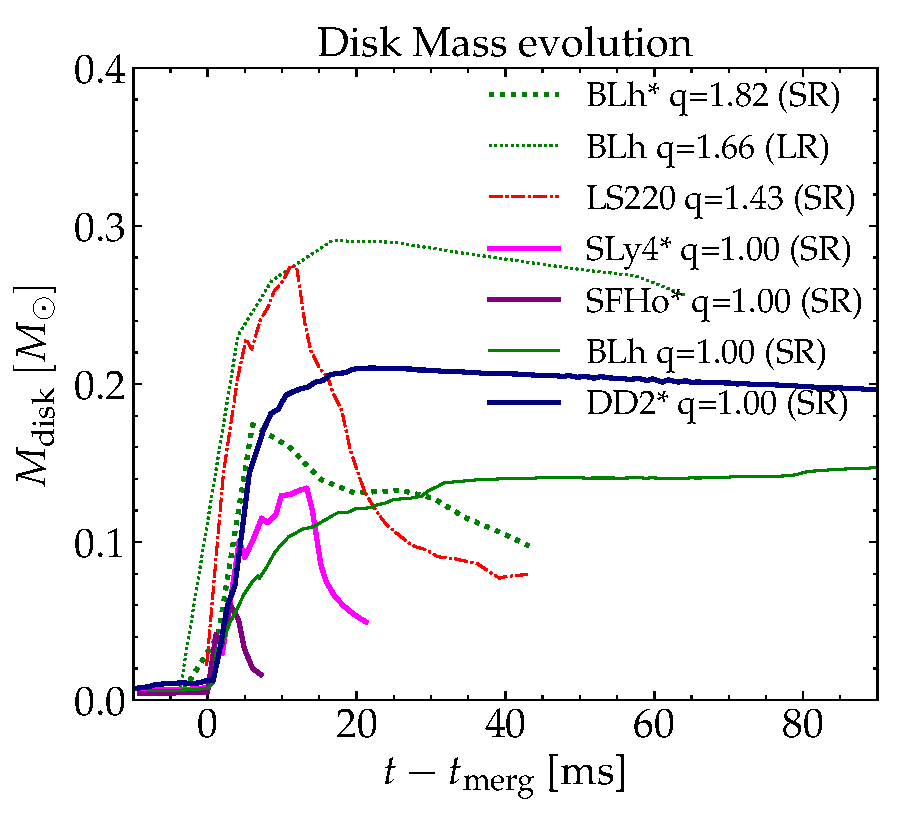
\includegraphics[width=0.49\textwidth]{disk/total_disk_mass_evo.pdf}
    \caption{Time evolution of the total disk mass for a few selected
        short-lived and long-lived cases. The former show a rapid 
        accretion right after disk formation. The plots show
        distinct difference in dynamical evolution after disk formation: accretion onto
        the newly formed BH (short-lived remnants) or accretion onto the NS
        remnant (DD2 $q=1$) with possible continuous mass shedding from the remnant
        into the disk (BLh* $q=1$). Adopted from \citet{Nedora:2020pak}
    } 
    \label{fig:disk_mass_evo}
\end{figure}


\subsection{Binaries with $q\lesssim1.4$}


Binaries with small mass ratio, ($q\lesssim1.4$) produce a \ac{MNS} remnant
that either survives on a dynamical timescale, set by the \ac{NS} rotation, before
collapsing to a \ac{BH}, or a \ac{MNS} that survives till the end of the simulations.
We refer to the former ones as \textit{short-lived} and the latter ones as 
\textit{long-lived} remnants.
Under the first category, fall the \ac{MNS} with relatively soft \ac{EOS}:
LS220 $q=1,1.1,1.2$, SFHo $q=1,1.1,1.4$ and SLy $q=1,1.1,1.4$. 
They collapse within $\sim20$~ms \pmerg. 
The exact time of the collapse however depends on the simulation resolution 
and on the inclusion of subgrid turbulence as was previosly noted by \citet{Radice:2017zta}.

\paragraph{Disk of short-lived remnants}

During the merger, shocks generated at the collisional interface of the \acp{NS} cores,
as well as, tidal torques exerted by the non axisymmetric remnant result in a formation
of the disk. 
Matter, energy and angular momentum are injected into the disk as the spiral density waves 
propagate outwards from the mass-shedding \ac{MNS} remnant 
\citep{Bernuzzi:2015opx,Radice:2018xqa}.
\red{HERE the letter stuff could be added, actually}

Within these waves the fluid reaches highest temperatures, which decrease rapidly, as 
disk expansion and neutrino emission cools the matter. 
In such a high-temperature environment, the electron-positron pair creation is enhanced.
%% [added from Shibata Review paper]
As a result, neutrons can capture positrons $n+e^+p\rightarrow\bar{\nu}_e$.
The average particle energies are large, close to the mass difference between neutron 
and proton. 
In combination with the high $\nu_e$ and $\bar{\nu}_e$ luminosities,
the large number of available positrons leads to an increase 
in the fluid electron fraction, $Y_e$ from that of the initially neutron-rich material
\citep{Qian:1996xt}.
Additionally, a \ac{MNS} is a strong neutrino emitter. The neutrino irradiation of the 
surrounding area alters its composition, and neutrino absorption takes place
$n+\nu_e\rightarrow p + e^{-}$ and $p + \bar{\nu}_e\rightarrow n + e^+$.
This drives the neutron and proton fraction towards equilibrium, and raises the $Y_e$.
\red{paper says: 
    The electron fraction is reset by an initial excess of electron antineutrino emission
    and electron neutrino absorption,}
The entropy per baryon varies between $3$ and $\lesssim 10\,$$k_{B}$/baryon \citep{Perego:2019adq}.
%% ---
If \ac{MNS} remnant collapses to a BH, the main source of neutrinos shuts down and 
the inner part of the disk is rapidly accreted. 
The disk then approaches quasi-steady state, Fig.~\ref{fig:disk_mass_evo}, with 
axisymmetric, approximately Keplerian profile.
The inner part of the resulted disk, at densities $\rho\sim10^{13}$~\gcm, 
is relatively hot, $T\sim10\,$ MeV, but neutron-rich $Y_e\sim0.1$, as it was shielded 
from the neutrino irradiation. The disk gets progressively colder and proton-rich 
outwards with $Y_e$ reaching $0.4$ at the edges.
%% ---
The disk mass at formation appears to depend on the \ac{NS} \ac{EOS}. Binaries with 
stiffer EOS (larger \ac{NS} radii) produce more massive disk.
\red{[Fitting function]
    The disk mass can be described within the numerical uncertainties by a
    quadratic function of the mass ratio and the reduced tidal
    parameters (see Sec.~\ref{sec:remdisk}).}
Additionally, the disk mass show a dependency on mass ratio. For instance, the most massive disks are formed in LS220 $q=1.43$ and  BLh $q=1.82$ models, where the latter experiences prompt collapse.
%% -- 
The disk accretionon a \ac{BH} removes up to $50\%$ of the disk mass on a timescale tens of milliseconds.


\paragraph{Disk of long-lived remnants}


If the \ac{MNS} is long-lived, the disk has time to complete its formation,
and thus it is more massive and extended \citep{Perego:2019adq}. 
As before, the disk is defined as matter, with $\rho\lesssim10^{13}$~\gcm. 
The disk mass increases with the mass ration and with stiffness of \ac{EOS}.
For instance, for BLh $q=1.00$ model, the disk mass reaches ${\lesssim}0.15\,\Msun$, 
while for DD2 $q=1.00$ model is exceeds ${\sim}0.2\,\Msun$.
For a models with BLh \ac{EOS}, the disk mass increases between $q=1.00$ and 
$q\sim1.4-1.5$ by a $100\%$.
%% ---
The long-term evolution of the disk is driven by its interaction with the \ac{MNS} 
remnant and cooling. 
And while in the case of a \ac{BH} remnant, the only possible interaction is the 
disk accretion onto a \ac{BH}, in case of a \ac{MNS} remnant the picture is more 
complex.
The disk neutrino cooling and gravitational pull from the remnant facilitates the 
accretion. However, generated at shocks, spiral density waves inject 
energy and angular momentum into the disk as well as centrifugally supported 
material (as \ac{MNS} undergoes mass-shedding). This heats up the disk and 
facilitates its expansion. 
In the figure  Fig.~\ref{fig:disk_mass_evo} the quasi-steady state disk accretion
is seen for the DD2 $q=1.00$ model. Meanwhile, in the BLh $q=1.00$ model, the 
mass-shedding by the remnant adds more material into the disk that it is being 
accretted. 
The analysis suggests, that this behaviour is due to two main factors: the 
very high average temperatures of the remnant and the disk achieved by this model, that 
are a consequence of the thermal effects included into the BLh EOS (\red{see sec.EOS}),
and the softness of the EOS, which lead to the strong oscillations of the 
remnant after merger (\red{see sec.DensyModes.}).

The inclusion of the subgrid turbulence smears the mass distribution of disk 
properties. The distributions of electron fraction, entropy per baryon and 
temperature appears broader. A more detailed quantitative analysis would require more 
simulations performed at several resolutions to disentangle the effects 
caused by the subgrid turbulence and by the finite grid \citep{Bernuzzi:2020txg,Radice:2020ids}.

\begin{figure}[t]
    \centering 
    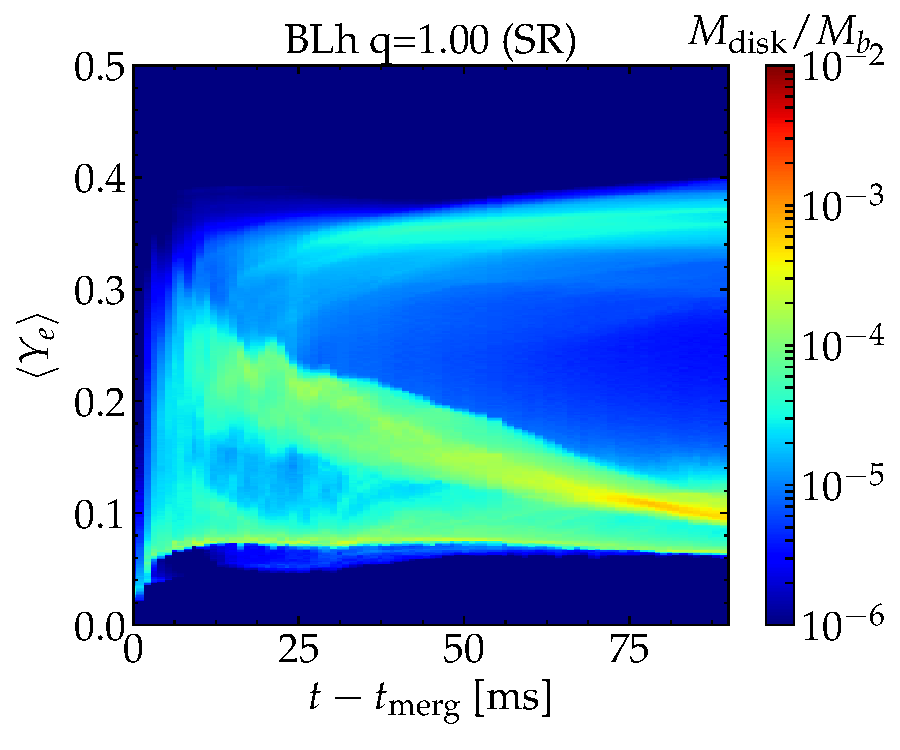
\includegraphics[width=0.49\textwidth]{disk/final_disk_timecorr_blh_q1_Lk.pdf}
    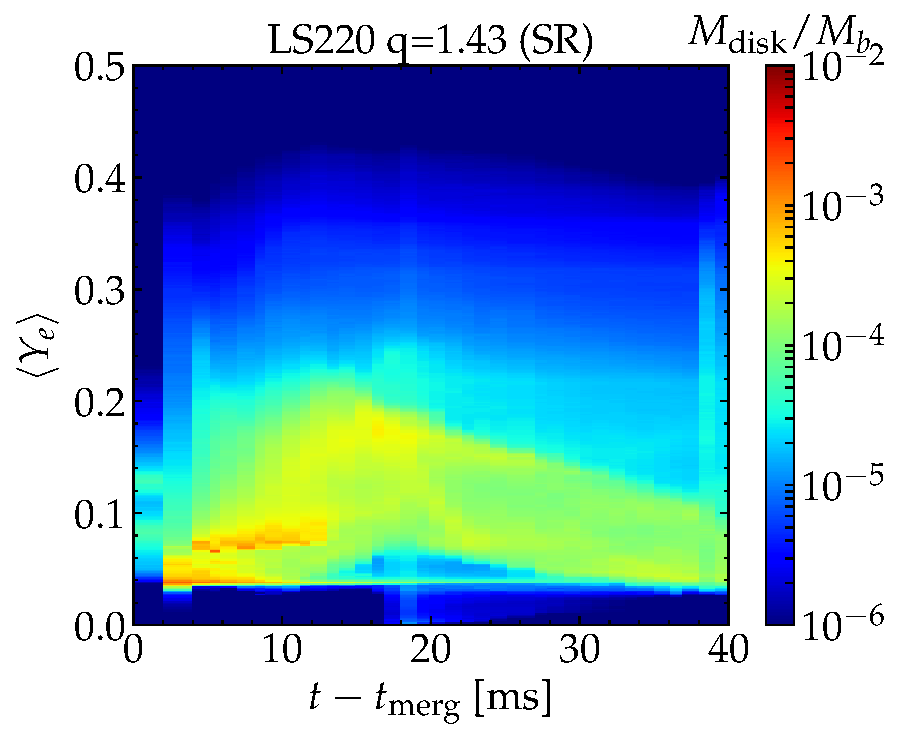
\includegraphics[width=0.49\textwidth]{disk/final_disk_timecorr_ls220_q14_LK.pdf}
    \caption{Evolution of the disk mass-averaged electron fraction with
        time for a long-lived (top) and a short-lived (bottom)
        remnant. The plot shows that with time the bulk of the disk lowers
        its $Y_e$ via cooling, while a small fraction in terms of mass
        gains a high $Y_e$, which relates to the highly 
        irradiated surface of the disk. Adopted from \citet{Nedora:2020pak}.
    }
    \label{fig:total_disk_time_corr_Ye_Blh_q1}
\end{figure}

\paragraph{Evolution of disk properties}

%% Ye evolution
The evolution of the mass-weighted electron fraction for the model
BLh $q=1.00$, the model that is evolved till $\sim 90$~ms after merger, 
is shown on the top panel of Fig.~\ref{fig:total_disk_time_corr_Ye_Blh_q1}.
%% --- 
During the formation, shock and spiral waves raises the disk electron fraction to
$Y_e\sim0.25$. As the disk evolves, the bulk of its mass, shielded from neutrinos, 
(Fig. \ref{fig:slice:heating_hu}, density contours) 
returns to neutron-rich condition with $Y_e\lesssim0.1$. 
The outer part of the disk, however, is subjected to the 
strong neutrino irradiation and reaches $Y_e\sim0.4$ of a timescale of ${\sim}40$~ms.
%% Note that neutrinos in merger remnants decouple at $\rho\sim10^{11}$~$\gccm$ \citep{Endrizzi:2019trv}. 
Notably, the apparent gap in the $Y_e$ distribution if Fig.~\ref{fig:total_disk_time_corr_Ye_Blh_q1} at $\langle Y_e \rangle \simeq 0.15$ 
might not be of physical origin, but an artifact from the neutrino M0 scheme, 
that assumes neutrinos propagate along the radial directions
(see sec.NEUt.M0.SCHEME), that is not well suited for capturing the 
neutrino emission and reabsorption from the disk midplane.
%% ---
In case of a short-lived model LS220 $q=1.43$ model 
(lower panel of the Fig.~\ref{fig:total_disk_time_corr_Ye_Blh_q1})
the average electron fraction is lower, as there is no strong neutrino 
emitter. Additionally, the outskirts of the more compact disk remain 
at low electron fraction as the neutrino emitted by the disk itself 
are the only source of neutrinos. 

\paragraph{Mass ejection on a long timescale}

As the disk expands and cools, the recombination of nucleons into 
alpha particles starts to take place.
The energy, released in recombination, might be sufficient for the outermost 
layers to become unbound, generating an outflow 
\citep{Beloborodov:2008nx,Lee:2009uc,Fernandez:2013tya}.
This processes however are expected to take place on a longer timescales,
that those that are simulated here.
On the $\sim100$~ms timescale, the outflows are driven by the neutrino heating, 
above the remnant, the so-called neutrino-driven wind 
(\nwind; \citealt{Dessart:2008zd,Perego:2014fma,Just:2014fka}),
and by the dynamical interactions between the \ac{MNS} 
remnant and the disk, the \swind{} \citep{Nedora:2019jhl}.
%% ---
We discuss the properties of the \nwind{} found in our simulations
in the section \red{sec.Ejecta.NuWind} and the properties of the 
\swind{} in the \red{sec.Ejecta.SWIND}.
%The \swind{} can have a mass up to
%a few $10^{-2}\,\Mo$ and velocities ${\sim}0.2$~c. The ejecta
%have electron fraction typically larger than ${\sim} 0.25$ since they are 
%partially reprocessed by hydrodynamic shocks in the expanding arms. 
%The \nwind{} is driven by neutrino heating above the remnant. It generates outflows
%with smaller masses ${\sim} 10^{-4}M_{\odot}$ and larger $Y_e$
%than the \swind{}. 
%Differently from \swind{} the mass flux of the \nwind{} in our simulations subsides 
%before the end of out simulations, due to rapid baryon loading of the 
%polar region.
%The \swind{} will be discussed in detail in Sec.~\ref{sec:spiralw}.
The effects of these outflows on the dynamical evolution of the remnant 
lies in the amount of mass and energy they can remove from the system.
Specifically, the \nwind{} have a typical mass of ${\sim} 10^{-4}\Msun$, 
while the \swind{} could remove $10^{-2}\,\Msun$ on a timescale of a $\sim100$~ms.

\begin{figure}[t]
    \centering 
    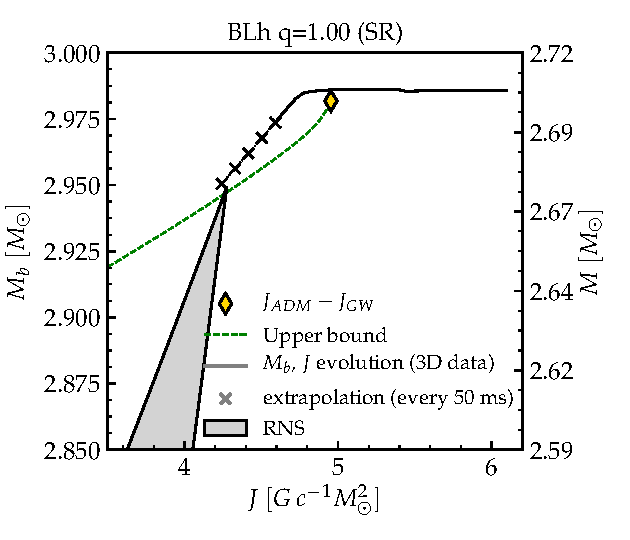
\includegraphics[width=0.49\textwidth]{ejecta_sec/secular_j_mb_RNS_blh.pdf}
    \caption{Baryon mass vs angular momentum diagram for the BLh $q=1$ remnant.
        The colored diamond marks the baryonic mass and angular momentum at the end
        of the dynamical gravitational-wave dominated phase.
        After the GW phase, the evolution is driven by the massive outflows.
        The solid black line is the $M_b$ and $J$ estimated from the 3D data
        integrals under the assumption of axisymmetry.
        The green dashed line is a conservative estimate
        of the mass ejection and a possible trajectory for the viscous
        evolution as estimated in \citet{Radice:2018xqa}. The crosses are
        a linear extrapolation in time of the solid black line. The gray
        shaded region is the region of stability of rigidly rotating NS equilibria.
        Adopted from \cite{Nedora:2020pak}
    }
    \label{fig:total_j_mb_rns_blh}
\end{figure}

To understand the remnant evolution on the timescales longer then the ones 
present here, requires ab-initio \ac{NR} simulations in $(3+1)D$ with compete physics.

Here we consider a BLh $q=1.00$ simulation, one of the longest runs we have performed.
After the merger, the \ac{MNS} remnant is born. With respect to the zero-temperature 
beta-equilibrium \ac{NS} configurations, the BLh $q=1.00$ 
remnant has an excess in baryon mass.
In the figure~\ref{fig:total_j_mb_rns_blh} we show the evolution of the 
total baryon mass, $M_b$, and total angular momentum, $J$, of the remnant.
As the total baryon mass is conserved (if there is no outflow), the early evolution 
of the remnant proceeds with $M_b=\text{const}$. The angular momentum is however 
lost by the remnant to emission of \acp{GW}. 
We evaluate the amount of angular momentum lost to \acp{GW} following the 
\citet{Damour:2011fu,Bernuzzi:2012ci,Bernuzzi:2015rla}.
\red{This has to be defined and noted that we use $\sim20$~ms postmerger mark
    and how exactly we compute all of it, the David's script
}
Substruct it from the initial data \ac{ADM} angular momentum we obtain the value 
that is left to the system after the \ac{GW} phase 
(the yellow marker on the Fig.~\ref{fig:total_j_mb_rns_blh}).
%% ---
Notably, after the \ac{GW} phase, the remnant still has an excess in angular momentum
in comparison with the rigidly rotating \ac{NS} configurations with the same baryon mass 
(gray triangular region in Fig.~\ref{fig:total_j_mb_rns_blh}).
We observe the same situation across all models \citep{Zappa:2017xba,Radice:2018xqa}.
\gray{
    On the angular momentum estimation:
    The radiated angular momentum (as well as energy) are computed from the 
    multipole loments $N_{lm}$ for the \ac{NR} complex "news function" at infinity. 
    The $J_{z;\text{rad}}(t)$ is computed as \citep{Damour:2011fu} 
    \begin{equation}
    \Delta J_{z\text{rad}}(t) \frac{1}{16}\sum_{l,m}^{l_{max}}\int_{t_0}^{t} dt' m \mathcal{L}[h_{lm}(t')(N_{lm}(t'))^*],
    \end{equation}
    where $h_{lm}$ is the multipolar metric waveform, 
    $N_{lm}(t) = dh_{lm}(t) / dt$, the news function, and $l_{max}=8$.
    The $J$ loss is metric dependent ($h$).
    The $h$ (strain???) is computed from $\Psi_4(t) = dN/dt = d^2h/dt^2$ by a 
    frequency-domain integration procedure with a low-frequency cut 
    $\omega_0 = 0.032/(m_1+m_2)$.
}
%% ---
The baryon mass of the remnant also exceeds maximum mass that a rigidly rotating 
equilibria could have.
Such remnant is generally referred to as a hypermassive neutron star (HMNS) following the 
nomenclature introduced for zero-temperature EOS equilibria \acp{NS} \citep{Baumgarte:1999cq}.
Such a remnant is expected to collapse to a BH. 
%% ---
However, a remnant can avoid the collapse by efficiently removing angular momentum
and mass and entering the rigidly rotating equilibria zone. 
%% ---
We compute the angular momentum and baryon mas evolution of the remnant, 
through volume integrals, assuming axisymmetry and evaluating the former using Eq.~\eqref{eq:method:ang_mom}, and the latter using the Eq.~\eqref{eq:method:mdisk}. 
The evolution of these two quantities is depicted with the black solid line if 
Fig.~\eqref{fig:total_j_mb_rns_blh}~\footnote{Note that the angular momentum estimated
    from the GW and from the integral of Eq.~\eqref{eq:method:ang_mom} assuming
    axisymmetry are compatible within the errors made in the latter estimate.
}.
We observed that after the \ac{GW} phase, the remnant continues to evolve, loosing the 
angular momentum together with the baryon mass. This is achieved through massive outflow,
the \swind{}. 
The extrapolation of the final trend of the mass and angular momentum loss shows, that 
if $\approx0.05\,\Msun$ ($\approx40$\% of the final disk at the end of simulation) is 
ejected, the \ac{MNS} remnant would approach the rigidly rotating equilibria region 
at the mass-shedding limit. Extrapolation indicates, that if the ejecta mass flux does 
not change, this would occur on a timescale of $\sim 300$~ms \pmerg{}.
Similar results are obtained with the conservative upper bound estimate on the 
evolution of the long-lived remnant (Eq.~$2$ in \citet{Radice:2018xqa}) (green dashed line in figure).
\red{WHAT the fuck is Keplerian limit, mass-shedding limit and rigidly rotating equilibria}
Additionally, while this simulation included the effects of turbulent viscosity on the
angular momentum transport, the ejecta could be further enhanced by the magnetic stresses 
\citep{Metzger:2006mw,Bucciantini:2011kx,Siegel:2017nub,Fernandez:2018kax,Ciolfi:2020hgg}.

Other simulations also produce a \ac{MNS} remnant with a similar evolutionary path. 
Models with DD2 \ac{EOS} however, are born with an excess in angular momentum, but not in 
baryon mass. They also evolve toward the rigidly rotating equilibria but slower.
Models with $q>1.00$ produce remnants that generally have larger excess in angular momentum 
and mass have how to shed a larger amount of mas to reach equilibrium configuration.
(\red{However we also show that these models tend to have stronger \swind{}, see sec.SPIRAL.WIND})
Overall, we estimate that for models with $q=1.00$ need to shed ${\sim}0.05\Msun$ while 
models with $q\eqsim 1.4$ need to remove $0.2\Msun$ to reach equilibrium configuration.



\section{Mass Ejection}



Tidal interactions and shocks exerted on the \acp{NS} at merger trigger the ejection of material
on the dynamical timescale. This is the \ac{DE} \citep[\eg][]{Hotokezaka:2013b,Bauswein:2013yna,Radice:2016dwd,Radice:2018pdn}. 



\subsection{Dynamical Ejecta}


%% The mechanism behind the dynamical ejecta [radice:2018pnd]
Tidal interactions and shocks exerted on the \acp{NS} at merger trigger the ejection of material
on the dynamical timescale. This is the \ac{DE} \citep[\eg][]{Hotokezaka:2013b,Bauswein:2013yna,Radice:2016dwd,Radice:2018pdn}. 

\red{More on the genral mechanism tidal vs shocked}
The \ac{DE} is evaluated with the geodesic criterion introduced in Sec.~\ref{sec:method:analysis:ejecta}.

Describe shock vs tidal components 

\subsubsection{Overall properties of the \ac{DE}}


The novelty of the set of models discussed in this thesis with respect to the 
previous study by \citet{Radice:2018pdn} is that all models include the neutrino heating via M0 scheme 
(see Sec.\ref{sec:theory:neutrino}) in addition to the neutrino cooling and for most models the effects 
of subgrid turbulence (see Set.\ref{sec:theory:grles}) are included.
Meanwhile, models cover a significantly more narrow range in 
dimensionless tidal deformability, $\tilde{\Lambda}$, and mass ratio, motivated by the \GW{}.

We can qulitativly asses the effects of neutrino heating by comparing the overall properties 
of our model set and that of the \citet{Radice:2018pdn}.
Specifically, the neutrino absorption leads to not only an increase in average electron 
fraction but also to larger total ejected mass and velocity. The latter two would be 
crucial for the non-thermal, kilonova afterglow (see Sec.\red{sec:KilonovaAfterglow}).

The mass averaged over the simulations from Tab.~\ref{tab:sim} is 
$\overline{\amd} = (3.442 \pm 2.495)\times 10^{-3}\,M_{\odot}$ (where
hereafter we report also the standard deviation), while the same
quantity calculated for data of \cite{Radice:2018pdn} 
is $\overline{\md} = (1.352\pm 1.250)\times 10^{-3}\,\Msun$.
The mass-averaged terminal velocity of the dynamical ejecta 
ranges between $0.1$c and $0.3$c, and in a good agreement with 
\cite{Radice:2018pdn}.
The mass-averaged velocity, averaged over all the simulations, is 
$\overline{\avd} = (0.172\pm0.038)\,{\text{c}}$.

We find that in our set of models, there is a correlation of $\avd$ with the tidal parameter 
$\tilde{\Lambda}$: the higher the $\tilde{\Lambda}$ the lower the $\avd$.
This can be understood from the general mechanism of the \ac{DE},
that tells in mergers of binaries with $q=1.00$, the shocked component of the ejecta 
is the dominant. The strength of shocks increases as the \acp{NS} become more compact 
(with decreasing $\tilde{\Lambda}$) and hence collide at higher velocities~\footnote{Note that in the definition of prompt collapse we adopted, there is no shocked ejecta.}.
%% ---
For binaries with high mass ration, however, the tidal component of the \ac{DE} is dominant. 
The velocity of the latter also is smaller for larger $\tilde{\Lambda}$, as stars collide 
at slower velocities due to their larger radii. 
%% ---
The mass-averaged electron fraction, $\ayd$, of our models lies the range $(0.1, 0.3)$
with an averaged value among all models $\overline{\ayd} = 0.175 \pm 0.063$.
Notably, the \citet{Radice:2018pdn} reported a more narrow range, $(0.1, 0.2)$.
This is a clear effect of the neutrino absorption included in our models, that elevates 
the everal electron fraction of the \ac{DE} as it is being irradiated by neutrinos 
during the merger.
Notably, the $\ayd$ of our models is close to those obtained with M1 
scheme of \citet{Sekiguchi:2016bjd} and \citet{Vincent:2019kor}.
%% ---
The effect of subgrid turbulence on the dynamical ejecta properties however,
found rather week and comparible to the effects of finite grid distritization 
\citep{Bernuzzi:2020txg,Radice:2020ids}.

We find that the properties of the \ac{DE} depends on the \mr{} and on the 
\ac{EOS} softness that can be parameterized with $\tilde{\Lambda}$. 
We investigate in detail the statistical properties of our set of models as well as 
other \ac{NR} \ac{BNS} data sets available in the literature in 
section \ref{sec:ejecta_disk_statisitcs}.





\subsection{Fast tail of the dynamical ejecta}

%\begin{figure}[t]
%    \centering 
%    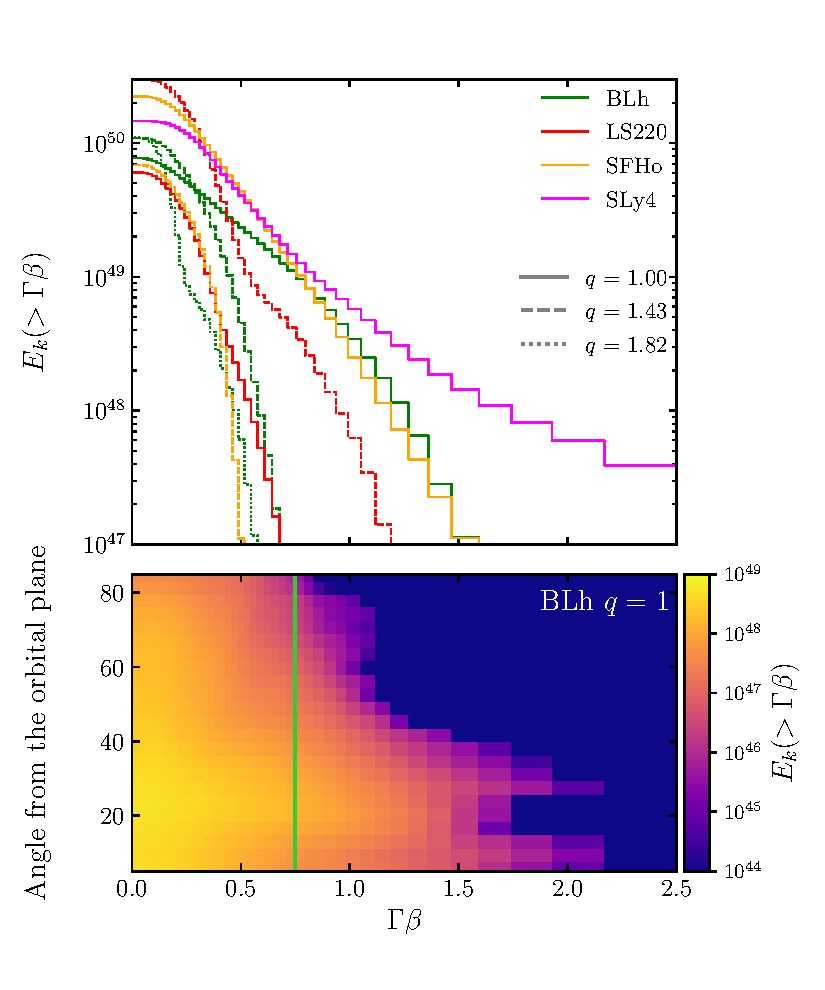
\includegraphics[width=0.49\textwidth]{./figs/kinetic_energy_struct_models.pdf}
%    \caption{
%        Total kinetic energy distribution for a selected set of models (\textit{top panel}) 
%        and angular distribution of kinetic energy for a BLh $q=1.00$ model (\textit{bottom panel}).
%        %% Also shown as a solid black line is the slow quasi-spherical model of \cite{Mooley:2017enz}.
%        The vertical light green line marks the $\upsilon_{\text{ej}}=0.6$.
%        The top panel shows that equal mass models have a more extend high energy tail,
%        while the bottom panel shows that the angular distribution of the ejecta is not 
%        uniform.
%        \red{Adopted from Nedora et al. (2021)}
%    } 
%    \label{fig:ejecta_vel_hist}
%\end{figure}
%
%The velocity distribution of \ac{DE} was found to include a very fast, 
%$\upsilon_{\text{ej}}\geq0.6$~c tail
%\cite{Piran:2012wd,Hotokezaka:2013b,Kyutoku:2012fv,Ishii:2018yjg,Hotokezaka:2018gmo,Radice:2018pdn}.
%%% ---
%The total mass of this tail was found to be dependent on the
%binary parameters and solution resolution,
%with an average $\sim 10^{-6}-10^{-5} M_{\odot}$.
%%% ---
%With respect to the fast tail origin, it can be divided into two main components 
%\citep{Radice:2018pdn}.
%The early component, that comprises the ejecta that is generated at the collisional interface 
%of two \acp{NS} of similar mass and directed primarily along the binary axes.
%And the late component that consist of matter that driven by the shock breakout from the ejecta 
%after the core bounce and confined mostly to the binary plane. 
%
%Among the simulations listed in \ref{tab:sim}, we select \red{XX} simulations 
%performed at standard resolution, and for which fast ejecta is found.
%%% ---
%Here we extract ejecta properties at the detector located at 
%$R=300G/c^2M_{\odot}\approxeq443$~km, from the merger, in agreement with \citet{Radice:2018pdn}.
%
%The mean value of the fast tail mass is
%
%\be\label{eq:ejecta:dyn:avg:M}
%\red{ \overline{\amd}(\upsilon>0.6) = (2.50 \pm 4.23)\times 10^{-5}M_{\odot}\ , }
%\ee
%
%where the standard deviation is also reported as an error.


%% ------------------ 
%% Note that the geodesic criterion above neglects the fluid's pressure and might
%% underestimate the ejecta mass. The Bernoulli criterion assumes that the (test
%% fluid) flow is stationary, so that there is a pressure gradient that can
%% further push the ejecta.  We find that both criteria predict dynamical
%% ejecta masses that are practically indistiguishable and well within the numerical uncertainties \citep{Bernuzzi:2020txg} if applied to extraction spheres at large coordinate radii; 
%% differences between the two criteria are instead present if they are applied to
%% matter volumes \citep[cf.][]{Kastaun:2014fna}.


\subsection{\swind{}}
\label{sec:spiralw}

\begin{figure*}[t]
    \centering 
    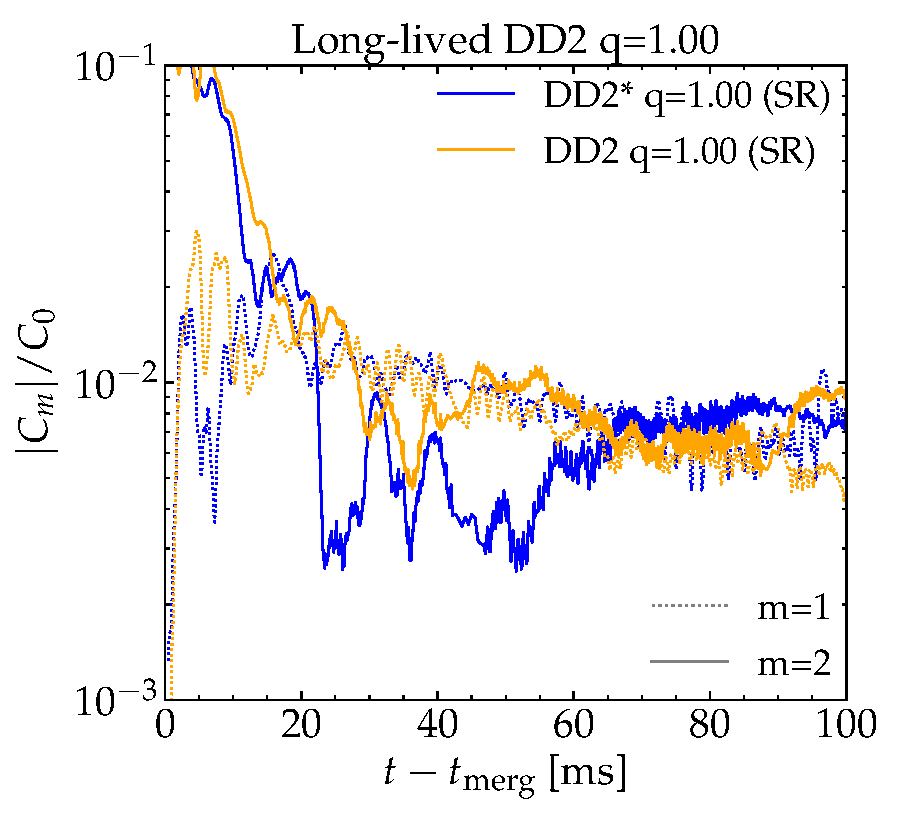
\includegraphics[width=0.49\textwidth]{remnant/dens_modes/modes_rho_dd2.pdf}
    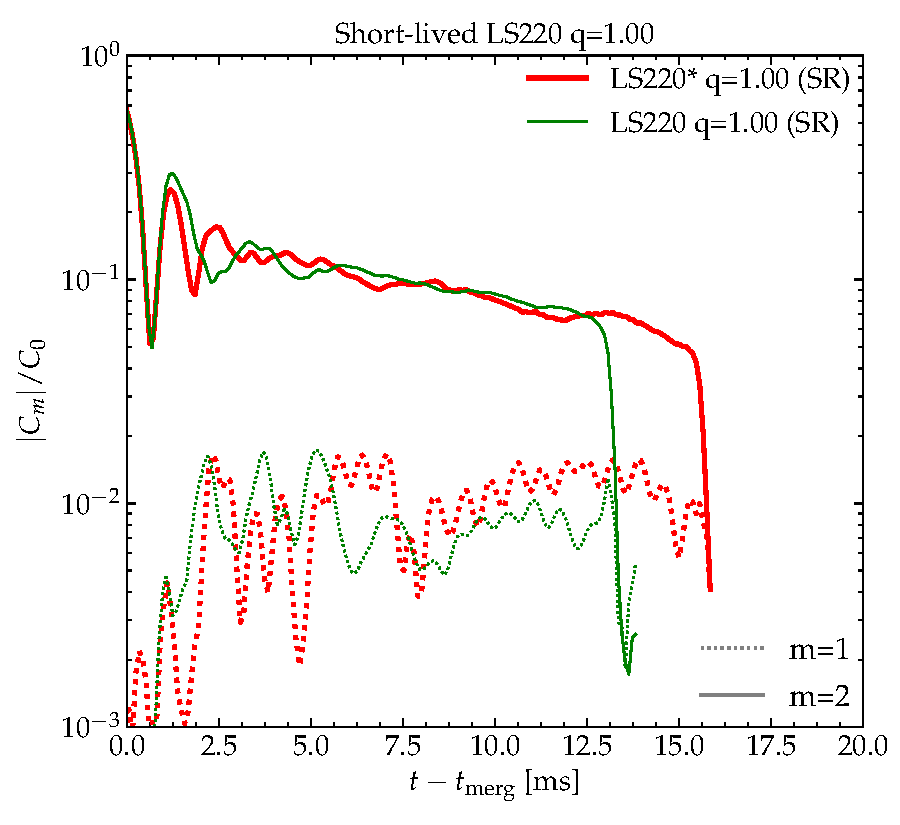
\includegraphics[width=0.49\textwidth]{remnant/dens_modes/modes_rho_ls220.pdf}
    \caption{Modes analysis for exemplary equal-mass long-live and short-lived
        remnants. The evolution of the $m=2$ and the $m=1$ monitored by
        Eq.~\eqref{eq:modes} is shown for the DD2 and LS220 remnant with and
        without turbulent viscosity. The $m=2$ mode in the long-lived
        remnant is strongly damped by the emission of gravitational
        radiation and becomes comparable to the $m=1$ mode on a timescale of
        ${\gtrsim}20\,$ms. Turbulent viscosity sustain the $m=2$ mode for
        a longer period. The $m=2$ mode is instead dominant to collapse in
        the short-lived remnant.
        (Adopted from \cite{Nedora:2020pak})
    }
    \label{fig:dens_modes}
\end{figure*}

Here we discuss the dynamics of spiral waves and the associated outflow, the \ac{SWW}.


\subsubsection{Remnant \& disk dynamics}


The hydrodynamical modes of the \ac{MNS} remnant are computed following the 
method described in Sec.\ref{sec:method:HDmodes}. 
The mode analysis is shown in the Fig.\ref{fig:dens_modes} for two representative 
simulations, the short-lived LS220 $q=1.00$ and the long-lived DD2 $q=1.00$.
The newly born \ac{MNS} remnant is not axisymmetric, displaying characteristic 
spiral arms, extending outwards from the shock interface of the collided cores 
\citep{Shibata:1999wm,Shibata:2006nm,Bernuzzi:2013rza,Kastaun:2014fna,East:2015vix,Paschalidis:2015mla,Radice:2016gym,Lehner:2016wjg}.
The bar-shaped, $m=2$ modes is the dominant one early in \pmerg{}, while the 
one-armed spiral $m=1$ modes stars to dominate in the late evolution 
\citep{East:2015vix,Paschalidis:2015mla,Radice:2016gym,Lehner:2016wjg,Bernuzzi:2013rza,Kastaun:2014fna}.
Indeed, the $m=2$ mode remains the dominant one until $\sim15-20$~ms \pmerg{}. 
After that, the LS220 $q=1.00$ model forms a \ac{BH}. 
In the DD2 $q=1.00$ model, however, the $m=1$ mode becomes comparable with $m=1$ 
throughout the remainder of the evolution, while the $m=2$ mode efficiently dissipates 
through \ac{GW} emission \citep{Bernuzzi:2015opx,Radice:2016gym}.
%% ---
We find that the magnitude of the $m=1$ mode increases with the binary \mr{}.
For instance the largest $C_{m=1}$ are found in BLh $q=1.43$ and LS220 $q=1.22$.
Stronger $m=1$ leads to more large \ac{SWW} mass flux.
The dependency of the $C_{m=2}$ on \mr{} however is not clear. 
This is in agreement with what reported by \citet{Lehner:2016wjg}.

Formation of the spiral arms is a generic hydrodynamic effect, that was identified 
in the \ac{NR} simulations with polytropic \ac{EOS} 
\citep{Bernuzzi:2013rza,Radice:2016gym}.
However, the evolution of these arms and quantitative behaviour of hydrodynamic
modes depends on the physics input. 
In the Fig.~\ref{fig:dens_modes} we show that the turbulent viscosity in the 
DD2 $q=1.00$ remnant stabilizes the $m=2$ mode, enhancing the angular momentum 
transport into the disk.
The $m=2$ mode, however, remains largely unaffected by the turbulent viscosity.
Similarly, the models' evolution in the LS220 $q=1.00$ is too short, for the 
subgrid turbulence to become important.

We compute the angular momentum of the \ac{MNS} remnant following the method,
discussed in Sec.\ref{sec:method:angmom}, where the remnant is distinguished 
from the disk on the basis of the rest mass density $\rho=10^{13}$~\gcm{} 
(see Sec.\ref{sec:method:diskdef}).
We find that for a long-lived rmnant 
on a timescale of $\sim20$~ms, about half of the total angular momentum 
of the \ac{MNS} remnant is transferred into the disk. 
%% [ from shibata review ]
This is a consequence of the fact that the remnant \ac{MNS} is strongly deformed 
after merger and gravitational torque on the surrounding matter, 
that allows for a rapid angular momentum transport.
%% ---
After, the remnant settles on quasi-stationary evolution path 
(see Sec.~\ref{sec:bns_dynsmics_overview}).

Following the disk and remnant mass evolution we observe, that the spiral 
density modes inject ${\sim}0.1-0.4\,\Msun$ of baryon mass into the disk during the 
first ${\sim}20$ms. 
The mass injection appears to be stronger for stiffer \acp{EOS}. 
With respect to the \mr{}, the higher $q$ binaries form a larger disc 
(see BLh* $q=1.82$ and LS220* $q=1.43$ on the Fig.~\ref{fig:disk_mass_evo}).

\begin{figure}[t]
    \centering 
    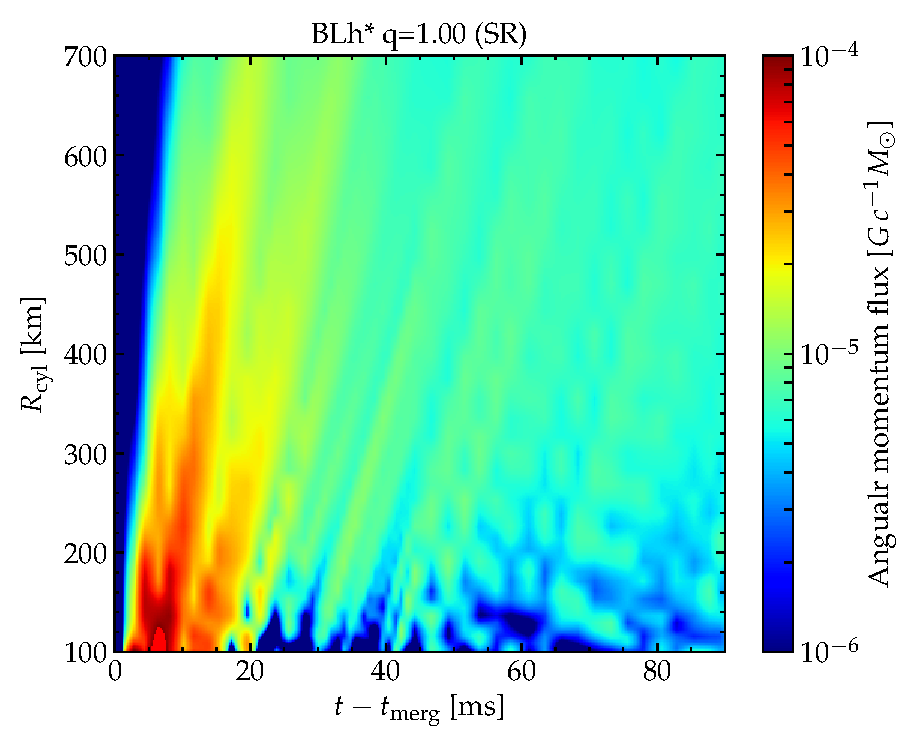
\includegraphics[width=0.49\textwidth]{remnant/evol_jflux_2d_BLh_M13651365_M0_SR_R1.pdf}
    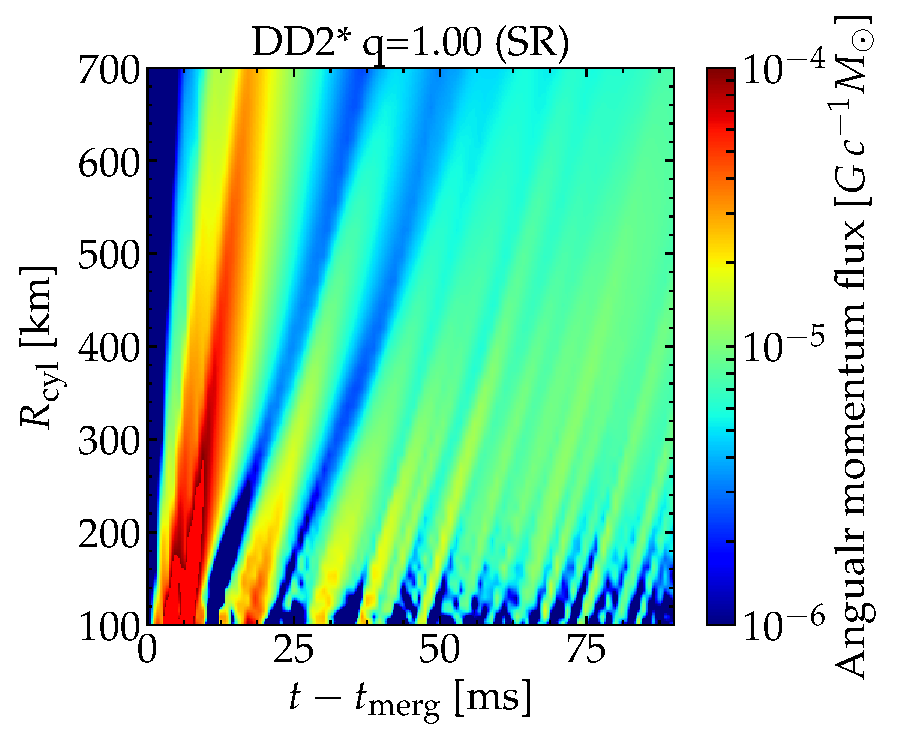
\includegraphics[width=0.49\textwidth]{remnant/evol_jflux_2d_DD2_M13641364_M0_SR_R1.pdf}
    \caption{Angular momentum flux through consecutive cylindrical
        surfaces identified by cylindrical radii from $R_{\text{cyl}}=100$ to $R_{\text{cyl}}=500$. The
        plot shows the angular momentum transport into the disk.
        Adapted from \citet{Nedora:2020pak}
    }
    \label{fig:disk_ang_mom_flux_map_blh_q1}
\end{figure}

In the Fig.~\ref{fig:disk_ang_mom_flux_map_blh_q1} we show how the 
angular momentum is being transported from the \ac{MNS} remnant into the disk
in two long-lived models with turbulent viscosity, DD2* $q=1.00$ and BLh $q=1.00$.
The angular momentum is transported via spiral waves that correspond do the 
hydrodynamic models, $m=1$ and $m=2$ discussed above.
We observer, that in the model with more stiff DD2 \ac{EOS},
the fist wave is stronger. Notably, the DD2* $q=1.00$ model 
also has a more massive disk.
%% --- 
Further, the evolution of the disk-remnant interactions 
after $\sim20$~ms \pmerg{} is different for two models. 
While the model with DD2 \ac{EOS} stops shedding mass into 
its disk and starts slowly accreting, the model with BLh \ac{EOS} continues to shed mass into the disk
(see Fig.~\ref{fig:disk_mass_evo} and discussion in
Sec.~\ref{sec:bns_dynsmics_overview})
The latter is caused by the strong angular momentum flux \red{actually the plot shows, that it is not}, emanating 
from the \ac{MNS} remnant and by the larger temperatures, 
that reached in the model with the BLh \ac{EOS}.
Larger temperatures leads to lower rotational frequency 
at which the mass shedding occurs \citep{Kaplan:2013wra}. 

The subgrid turbulence enhances the angular momentum transport. However more simulations of long-lived 
\ac{MNS} remnants are needed to asses the effects of the 
subgrid turbulence and \mr{} systematically. 

\begin{figure}[t]
    \centering 
    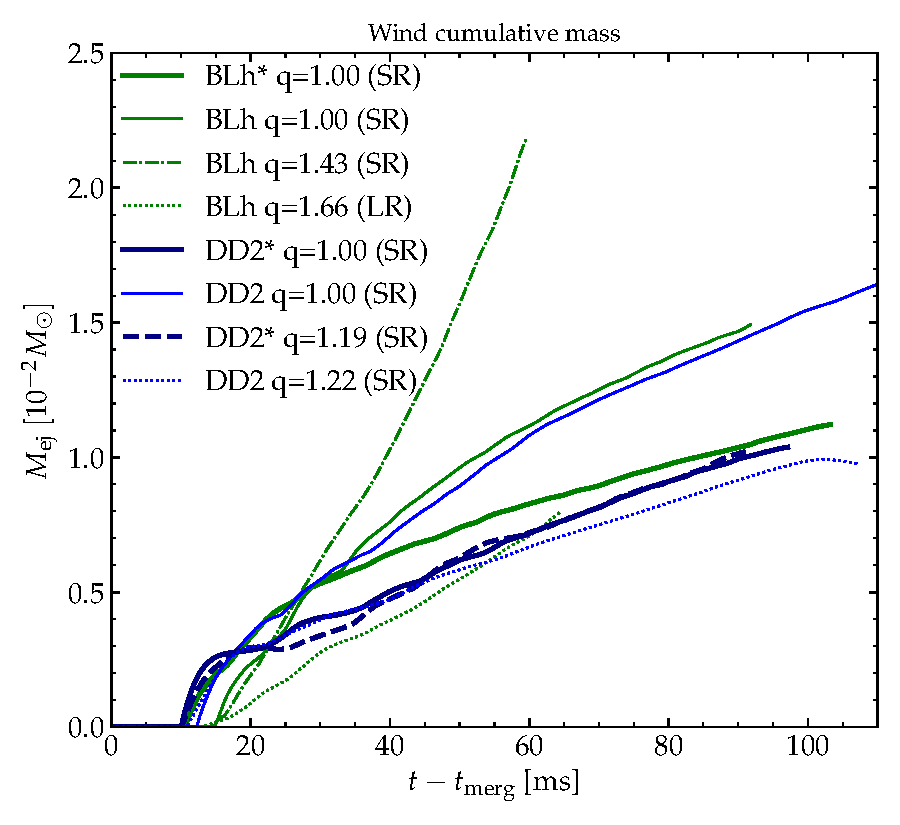
\includegraphics[width=0.50\textwidth]{ejecta_postdyn/wind_mass_flux.pdf}
    \caption{Cumulative mass of the \swind{} from long-lived
        remnants. The wind persists on timescales of $\O(100)\,$~ms with
        mass fluxes ${\sim}0.33-1.23\,\Msun/s$.
        Adapted from \citet{Nedora:2020pak}.
    }
    \label{fig:mej:bern}
\end{figure}

\begin{figure*}[t]
    \centering 
    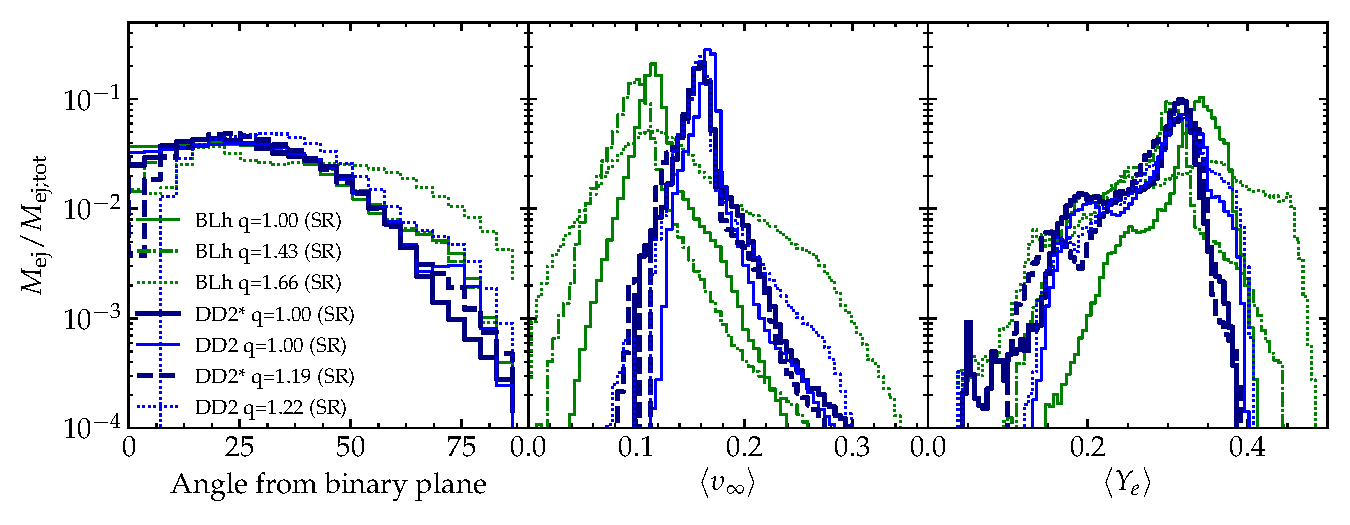
\includegraphics[width=0.99\textwidth]{ejecta_postdyn/wind_hists_shared.pdf}
    \caption{Mass-averaged histograms of the \swind{} for a selected
        subset of long-lived remnant. From left to right: ejecta angular
        distribution, ejecta terminal velocity and electron
        fraction. Remnants from more asymmetric binaries produce winds
        with broader angular distribution.
        The \swind{} from the DD2 EOS remnants has larger velocities
        then the winds from the softer BLh EOS. The electron fraction
        peaks at ${\sim}0.3$ and it is distributed from $0.1$ to $0.4$.
        Adapted from \citet{Nedora:2020pak}.
    }
    %
    \label{fig:ejecta:bern:hist}
\end{figure*}

%% --------------------------------
%% TAB WIND SUMMARY
\begin{sidewaystable}
%\begin{table*}[t]
  \centering
  \captionsetup{width=1.0\linewidth}
  \caption{%
    Summary table of the \swind{} properties of long-lived remnants. The columns contain
    the following information, starting from the left. Equation of
    state, mass-ratio, available resolutions,
    inclusion of subgrid turbulence, time of the
    simulation end, mass of the
    \swind{}, mass-loss rate via \swind, mass-averaged electron fracton, terminal
    velocity and, finally, RMS angle for \swind{}. For these four
    quantities we give the mean value among the resolutions and
    one-sigma deviations. For binaries for which only one
    resolution is present, the error is assumed to be $20\%$ of the value.
    (Adapted from \cite{Nedora:2020pak}).
    }
  \label{tab:spiralwavewind}
  \begin{tabular}{c c c c c c c c c c}
    \hline\hline
    EOS & $q$ & Resolution & GRLES & $t_{\text{end}}$ & $\amw$ & $\amw/\Delta t$ & $\ayw$ & $\avw$ & $\langle \theta_{\text{ej}}^{\text{w}} \rangle$ \\
    &   &   &   & [ms] & $[10^{-2} M_{\odot}]$ & $[M_{\odot}/s]$ &   & $[c]$ &   \\ 
    \hline
    \hline
    BLh & 1.00 & \texttt{SR HR LR} & \cmark & $43.3$ $91.8$ $23.1$ & $0.39^{+0.07} _{-0.07} $ & $0.70^{+0.32} _{-0.32} $ & $0.31^{+0.01} _{-0.01} $ & $0.12^{+0.01} _{-0.01} $ & $27.06^{+2.61} _{-2.61} $ \\
    BLh & 1.00 & \texttt{SR} & \xmark & $ $ $103.2$ $ $ & $1.12^{+0.57} _{-0.57} $ & $1.07^{+0.21} _{-0.21} $ & $0.34^{+0.01} _{-0.01} $ & $0.12^{+0.02} _{-0.02} $ & $15.72^{+2.00} _{-2.00} $ \\
    \hline
    BLh & 1.18 & \texttt{LR} & \cmark & $69.4$ $ $ $ $ & $1.28^{+0.64} _{-0.64} $ & $1.23^{+0.25} _{-0.25} $ & $0.33^{+0.01} _{-0.01} $ & $0.11^{+0.02} _{-0.02} $ & $14.98^{+2.00} _{-2.00} $ \\
    \hline
    BLh & 1.43 & \texttt{LR SR} & \cmark & $35.1$ $59.6$ $ $ & $0.75^{+0.18} _{-0.18} $ & $1.06^{+0.67} _{-0.67} $ & $0.27^{+0.01} _{-0.01} $ & $0.09^{+0.01} _{-0.01} $ & $19.43^{+2.22} _{-2.22} $ \\
    \hline
    BLh & 1.54 & \texttt{LR} & \cmark & $45.8$ $ $ $ $ & $0.63^{+0.32} _{-0.32} $ & $0.44^{+0.09} _{-0.09} $ & $0.32^{+0.01} _{-0.01} $ & $0.10^{+0.02} _{-0.02} $ & $21.46^{+2.00} _{-2.00} $ \\
    \hline
    BLh & 1.66 & \texttt{LR SR} & \cmark & $64.6$ $20.1$ $ $ & $0.12^{+0.09} _{-0.09} $ & $0.37^{+0.34} _{-0.34} $ & $0.33^{+0.05} _{-0.05} $ & $0.13^{+0.01} _{-0.01} $ & $52.08^{+20.89} _{-20.89} $ \\
    \hline
    \hline
    DD2 & 1.00 & \texttt{LR SR HR} & \cmark & $123.0$ $113.0$ $74.4$ & $1.25^{+0.14} _{-0.14} $ & $1.30^{+0.19} _{-0.19} $ & $0.30^{+0.01} _{-0.01} $ & $0.17^{+0.00} _{-0.00} $ & $14.88^{+0.87} _{-0.87} $ \\
    \hline
    DD2 & 1.20 & \texttt{LR SR HR} & \xmark & $37.3$ $91.0$ $55.2$ & $0.48^{+0.09} _{-0.09} $ & $0.74^{+0.24} _{-0.24} $ & $0.26^{+0.01} _{-0.01} $ & $0.15^{+0.00} _{-0.00} $ & $24.54^{+2.23} _{-2.23} $ \\
    \hline
    DD2 & 1.43 & \texttt{LR SR} & \cmark & $37.7$ $62.0$ $ $ & $0.60^{+0.02} _{-0.02} $ & $0.51^{+0.06} _{-0.06} $ & $0.23^{+0.12} _{-0.12} $ & $0.16^{+0.00} _{-0.00} $ & $21.74^{+0.03} _{-0.03} $ \\
    \hline
    \hline
    SFHo & 1.43 & \texttt{SR} & \cmark & $ $ $46.5$ $ $ & $0.58^{+0.30} _{-0.30} $ & $0.43^{+0.09} _{-0.09} $ & $0.31^{+0.01} _{-0.01} $ & $0.17^{+0.02} _{-0.02} $ & $22.67^{+2.00} _{-2.00} $ \\
    \hline
    \hline
    SLy4 & 1.43 & \texttt{SR} & \cmark & $ $ $40.3$ $ $ & $0.53^{+0.27} _{-0.27} $ & $0.38^{+0.08} _{-0.08} $ & $0.29^{+0.01} _{-0.01} $ & $0.18^{+0.02} _{-0.02} $ & $23.52^{+2.00} _{-2.00} $ \\
    \hline\hline
\end{tabular}
%\end{table*}
\end{sidewaystable}

%% --------------------------------


\subsubsection{Properties of the \swind{}}


Density waves, propagating outwards through the disk induce the outflow, the \ac{SWW} 
\citep{Nedora:2019jhl}.

\red{HERE THE LETTER STUFF COULD GO}

The \ac{SWW} is estimated following the Bernoulli criterion as described in 
the Sec.~\ref{ec:method:analysis}. 
We start to follow the \ac{SWW} after the \ac{DE} has saturated. 

We report the overall properties of the \ac{SWW} for all the models with the 
long-lived \ac{MNS} remnant that were also evolved for a sufficiently long time 
in the Tab.~\ref{tab:spiralwavewind}. 
The time evolution of the total mass of the \ac{SWW} is shown in the Fig.~\ref{fig:mej:bern}.
We observe that in all simulations \acp{SWW} persists till end without saturation.
This is because the outflow is driven by the angular momentum and mass transport 
induced by the dynamical instabilities in the remnant, the $m=1,2$ modes, discussed 
above. And as the $m=1$ modes are not efficiently damped \citep{Paschalidis:2015mla,Radice:2016gym,Lehner:2016wjg,East:2016zvv},
the \ac{SWW} could theoretically continue until the system collapses to a \ac{BH} 
or reaches the equilibrium (Sec.~\ref{sec:bns_dynsmics_overview}).

The strongest \ac{SWW} is found in binaries with $q>1$, such as 
$q=1.67$ and LS220 $q=\red{1.4}$. 
With the mass-loss rate ${\sim}0.5\, \Msun/{\text{s}}$, these models can eject 
${\sim}0.02\,\Msun$ within ${\sim}50$~ms of \pmerg{} evolution.
We find that as the \ac{EOS} becomes softer, lower \mr{} is needed to achieve high 
mass flux. For instance, the \ac{SWW} mass flux for BLh* $q=1.66$ is achieved by the 
model LS220* with $q=1.22$. 
A possible explanation for this is that the models with softer \ac{EOS} have stronger 
$m=1$ modes in the remnant (see Sec. \ref{sec:remdisk}).
When \ac{MNS} remnant collapses to a \ac{BH} and the mechanism that injects angular 
momentum into the disk shuts down, the \ac{SWW} mass flux subsides. 
Thus, the total ejected mass via \ac{SWW} is directly related  o the lifetime of the 
\ac{MNS} remnant, an addition to the binary parameters, \ac{EOS} and \mr{}.

The \ac{SWW} mass flux depends on the disk configuration, as more extended disks 
have outer layers that are less gravitationally bound. In turn, the disk 
configuration is dependent on the thermal effects. Higher temperature leads to 
stronger thermal pressure that increases the disk size. 
However, the dependency of the \ac{SWW} mass flux on the stiffness of the \ac{EOS} 
appears to be stronger, as the stiffer \ac{EOS} leads to a more massive disk 
(Sec.~\ref{sec:overview}). More simulations with longer postmerger evolution are needed 
to make a quantitative assessment. 
Overall the \swind{} from the long-lived remnant has a mass flux $\geq 0.4\, \Msun/{\text{s}}$.

We find that the properties of the \ac{SWW} depend only weakly on the binary parameters,
\mr{} and \ac{EOS}.The mass-histograms of the wind angular distribution, velocity and 
electron fraction are displayed in Fig.~\ref{fig:ejecta:bern:hist}. 
The angular distribution of the \ac{SWW} is similar to that of the \ac{DE}. The ejecta 
has a broad distribution around the binary plane.
The \ac{SWW} has a high average electron fraction, with the overall 
broad distribution of $0.1\lesssim \ayw\lesssim0.4$ that peaks at ${\sim}0.35$.
The low electron fraction material originates primarily at early times, when the 
material did not have enough time to be processed by neutrinos and before the 
outflow reaches quasi-steady state.
The \ac{SWW} average velocity is higher for stiffer \ac{EOS}, with the peak 
of the distribution laying between ${\sim}0.1\,$c and ${\sim}0.2\,$c.
However, more simulations of the \ac{MNS} remnants long-term evolution are 
required to confirm and quantitatively investigate this trend.
However, if it is indeed a generic feature, then it might imply 
an EOS dependent distinct feature in the electromagnetic counterpart. 
In particular, the observation of a fast blue kN given by the \swind{}
should be associated to a stiff EOS.

%% It is however expected, that as the system becomes more stationary and larger part 
%% of the disk accrets on the \ac{MNS} the outflow should subside. 


\subsection{\nwind{}}

\begin{figure*}[t]
    \centering 
    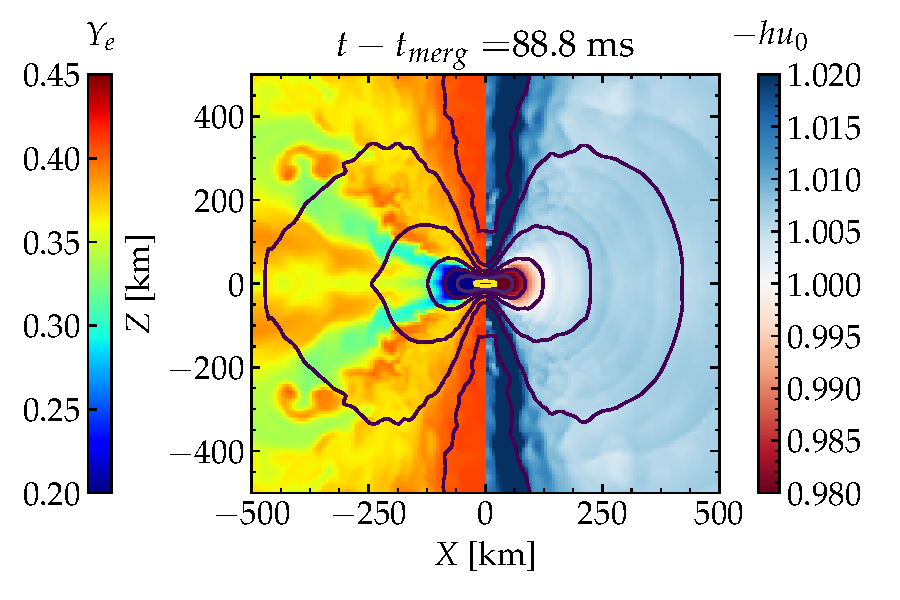
\includegraphics[width=0.49\textwidth]{slices/slice_xz_ye_hu_1.pdf}
    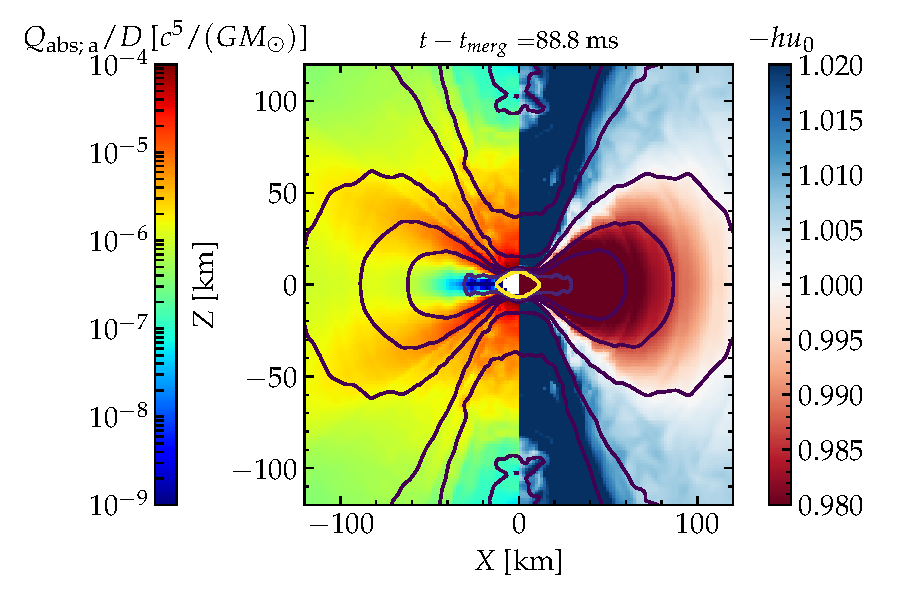
\includegraphics[width=0.49\textwidth]{slices/slice_xz_abs_energy_hu_3.pdf}
    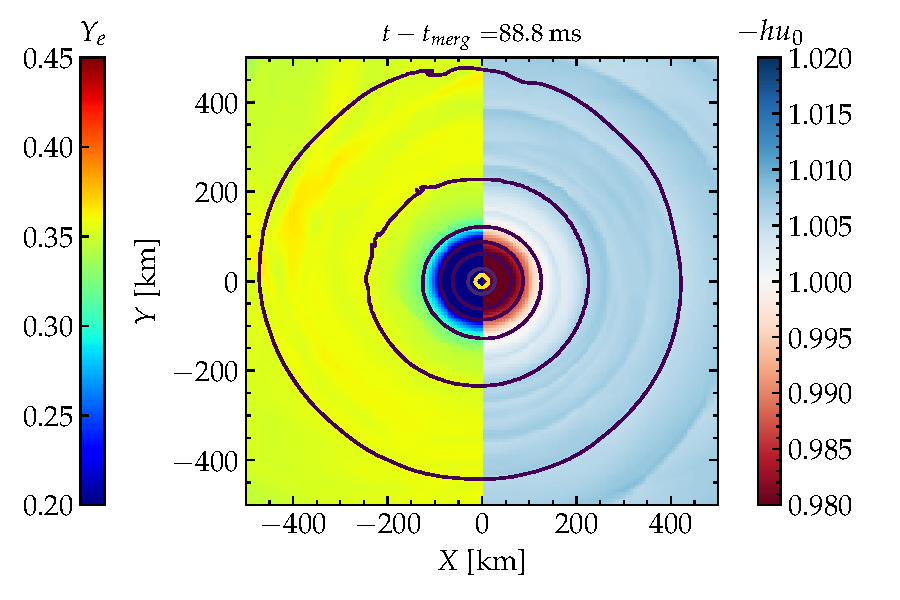
\includegraphics[width=0.49\textwidth]{slices/slice_xy_ye_hu_1.pdf}
    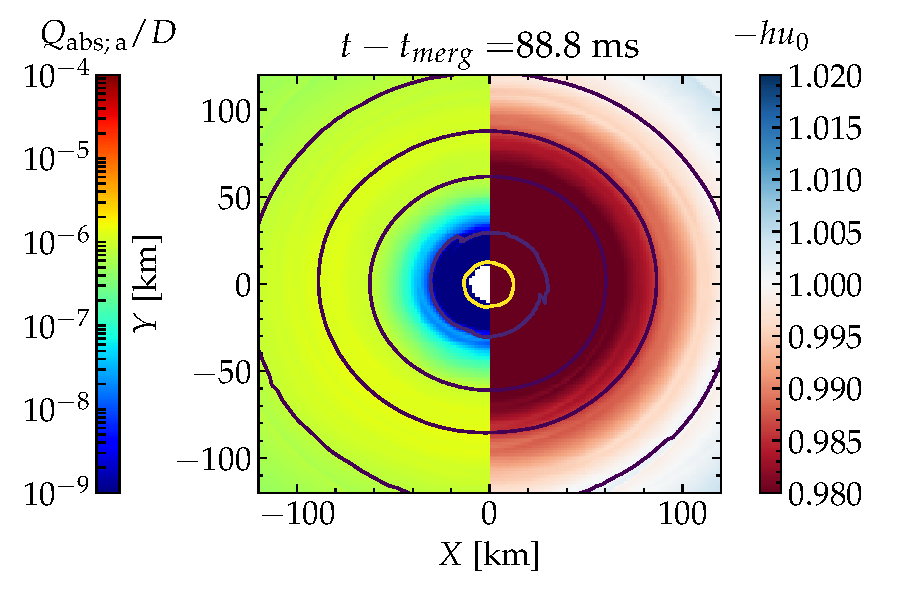
\includegraphics[width=0.49\textwidth]{slices/slice_xy_abs_energy_hu_3.pdf}
    \caption{Snapshot of the $(x,z)$ and $(x,y)$ slices of the BLh $q=1$ model at 
        ${\sim}89\,$ms after merger. Left panels: electron fraction and
        $-hu_0$. High $Y_e$ values indicate neutrino
        postprocessing and irradiation. The $-hu_0>1$ indicates the
        material that gains enough energy to become unbound at
        infinity. 
        %
        Right: $-hu_0$ and the absorption energy rate $Q_{\text{abs};\:\bar{\nu}_e}$ 
        of electron antineutrinos normalized to the fluid density $D$.
    }
    %
    \label{fig:slice:heating_hu}
\end{figure*}

In this section we investigate in detail the 
high electron fraction, polar component of the \acp{SWW}.
We propose that this outflow is mostly driven by the neutrino 
reabsorption, rather than by the dynamical mechanism responsible for the bulk of the 
\ac{SWW}.

The presence of the baryonic winds developing on the timescale of $\mathcal{O}(10)$~ms
and driven by the neutrino absorption above the remnant, where the neutrino flux is strong 
was reported before \citep[\eg][]{Perego:2014fma}. 

In this section we focus of the feducial model BLh $q=1.00$ (SR). 

In the left column of plots in Fig.~\ref{fig:slice:heating_hu} we compare 
the the Bernoulli parameter, 
$-hu_t$ (see Sec.\ref{sec:method:Bernoulli}), and the fluid electron 
fraction. 

In the right column of plots in Fig.~\ref{fig:slice:heating_hu} we compare 
the the Bernoulli parameter with the heating energy rate due to electron anti-neutrino absorption 
$Q_{\text{abs};\:\bar{\nu}_e}$ (see Sec.~\ref{method:M0:eq_for_Q}) divided by with 
$D=W\rho\sqrt{\gamma}$ (fluid's conserved rest-mass density)
We observe that the electron fraction in the polar region with angle 
from binary plane $\theta>60^{\circ}$ reaches $Y_e\sim0.35$ due to the absorption of 
electron-type neutrinos.
The strongest neutrino heating occurs in the vicinity of the remnant at densities 
$\rho\sim10^{11}$~\gcm, that roughly correspond to the region where neutrinos decouple,
the so-called neutrinosphere \citep{Endrizzi:2019trv}.

In Fig.~\ref{fig:slice:heating_hu} we compare the Bernoulli parameter, 
$-hu_t$ (see Sec.\ref{sec:method:Bernoulli}), that is always plotted 
on the right half of a panel, with the electron fraction (left 
column of plots and heating energy rate due to electron anti-neutrino absorption 
$Q_{\text{abs};\:\bar{\nu}_e}$ divided by with $D=W\rho\sqrt{\gamma}$ 
(fluid's conserved rest-mass density).
The observed correlation between the $E_\nu/D$ \red{???} and $-h u_t$ further suggests, 
that the outflow around the polar axis is driven by the neutrino absorption. 
Additionally, we found that if the neutrino absorption is not included into the 
simulation, \eg, using leakage only, the \nwind{} is absent. 
%% --- 
The collimated polar outflow can be further boosted and stabilized by the presence of the 
strong magnetic fields \citep{Bucciantini:2011kx,Ciolfi:2020hgg,Mosta:2020hlh}.
%% ---
Notably, there is not clear distinction between the \nwind{} and \ac{SWW}, especially 
at the intermediate latitudes ($\theta \sim 45^{\circ}$), where both mechanisms types of 
ejecta are present, and both, neutrino absorption and dyanmical effects driving the \ac{SWW} 
are contributing. 
%% --- 
In order to compute the mass flux of the \nwind{} an additional criterion is required. 
We consider two physically motivated criteria, the geometrical, flaggin the part of the \ac{SWW} 
and \nwind{} if it is polar, \ie, $\theta>60^{\circ}$, and the composition criterion, $Y_e > 0.35$.
%% --- 
We find that the \nwind{} is not a steady state outflow, contrary to the bulk of the \ac{SWW}.
After the initial strong rise, the mass flux rapidly decays in time, and for most models stops 
by the end of the simulations. This behaviour is independent of the criterion we use. 
We attribute it to the rise of the baryon loading above the remnant as the material gets lifted 
by thermal pressure from the disk.
The total mass of the \nwind{} is ${\sim}10^{-3}-10^{-4}M_{\odot}$. Its properties resemble those 
reported in e.g. \citet{Dessart:2008zd,Perego:2014fma,Fujibayashi:2020dvr}
Notably, in some of the works, the \nwind{} was found to require longer timescales to develop, 
achieving the quasi-steady state. 
This can be attributed to the strict criteria to isolate the \nwind{} and by the absence of the 
\ac{SWW} in other works. 
Additionally, our simulations might not be sufficiently long to achieve the donditions 
sufficient for the development of the quasi-steady state \nwind{}.
%% Additionally, as our models are at most $\sim100$~ms long, the conditions required for the steady 
%% state \nwind{} might not been achieved.


%% =======================================================
%%
%%                   Disc structure
%%
%% =======================================================


\section{Remnant disk structure}

\begin{figure}[t]
    \centering
    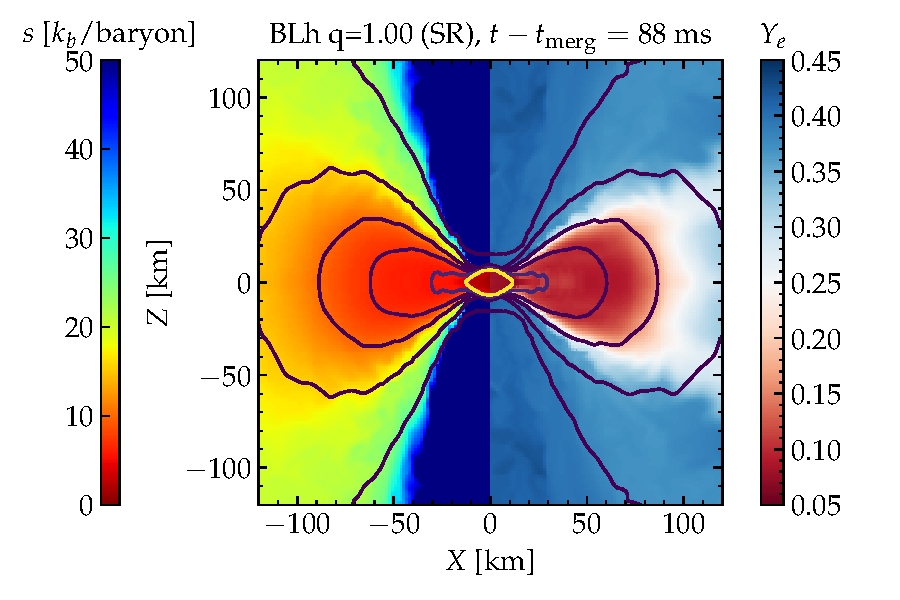
\includegraphics[width=0.49\textwidth]{disk/final_structure/slice_xz_entr_ye_blh_q1_rl3.pdf}
    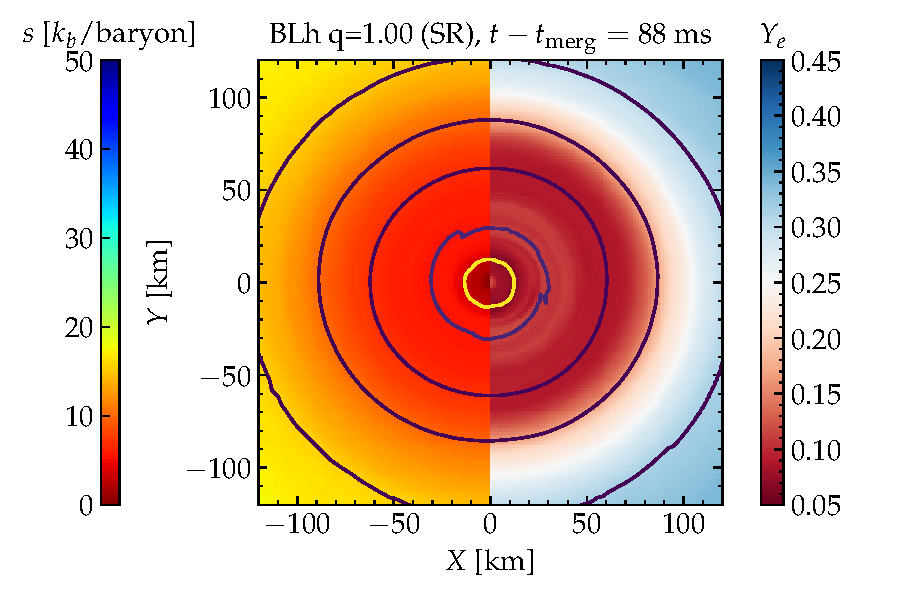
\includegraphics[width=0.49\textwidth]{disk/final_structure/slice_xy_entr_ye_blh_q1_rl3.pdf}
    \caption{Entropy and electron fraction on the $(x,z)$ (top) and
        $(x,y)$ planes (bottom) for the remnant of BL $q=1$ at the end
        of the simulation. Each plot is divided vertically, with entropy
        being color-coded on the left and electron fraction on the
        right. Solid contours stand for rest muss density. Counting from
        the center, the values are $[10^{13}, 10^{12}, 10^{11}, 10^{10},
        10^{9}]$ g cm$^{-3}$, with the inner most contour encompassing
        the remnant.
        (Adapted from \citet{Nedora:2020pak})
    }  
    \label{fig:snapshots_xy_ye_entr}
\end{figure}

\begin{figure*}[t]
    \centering 
    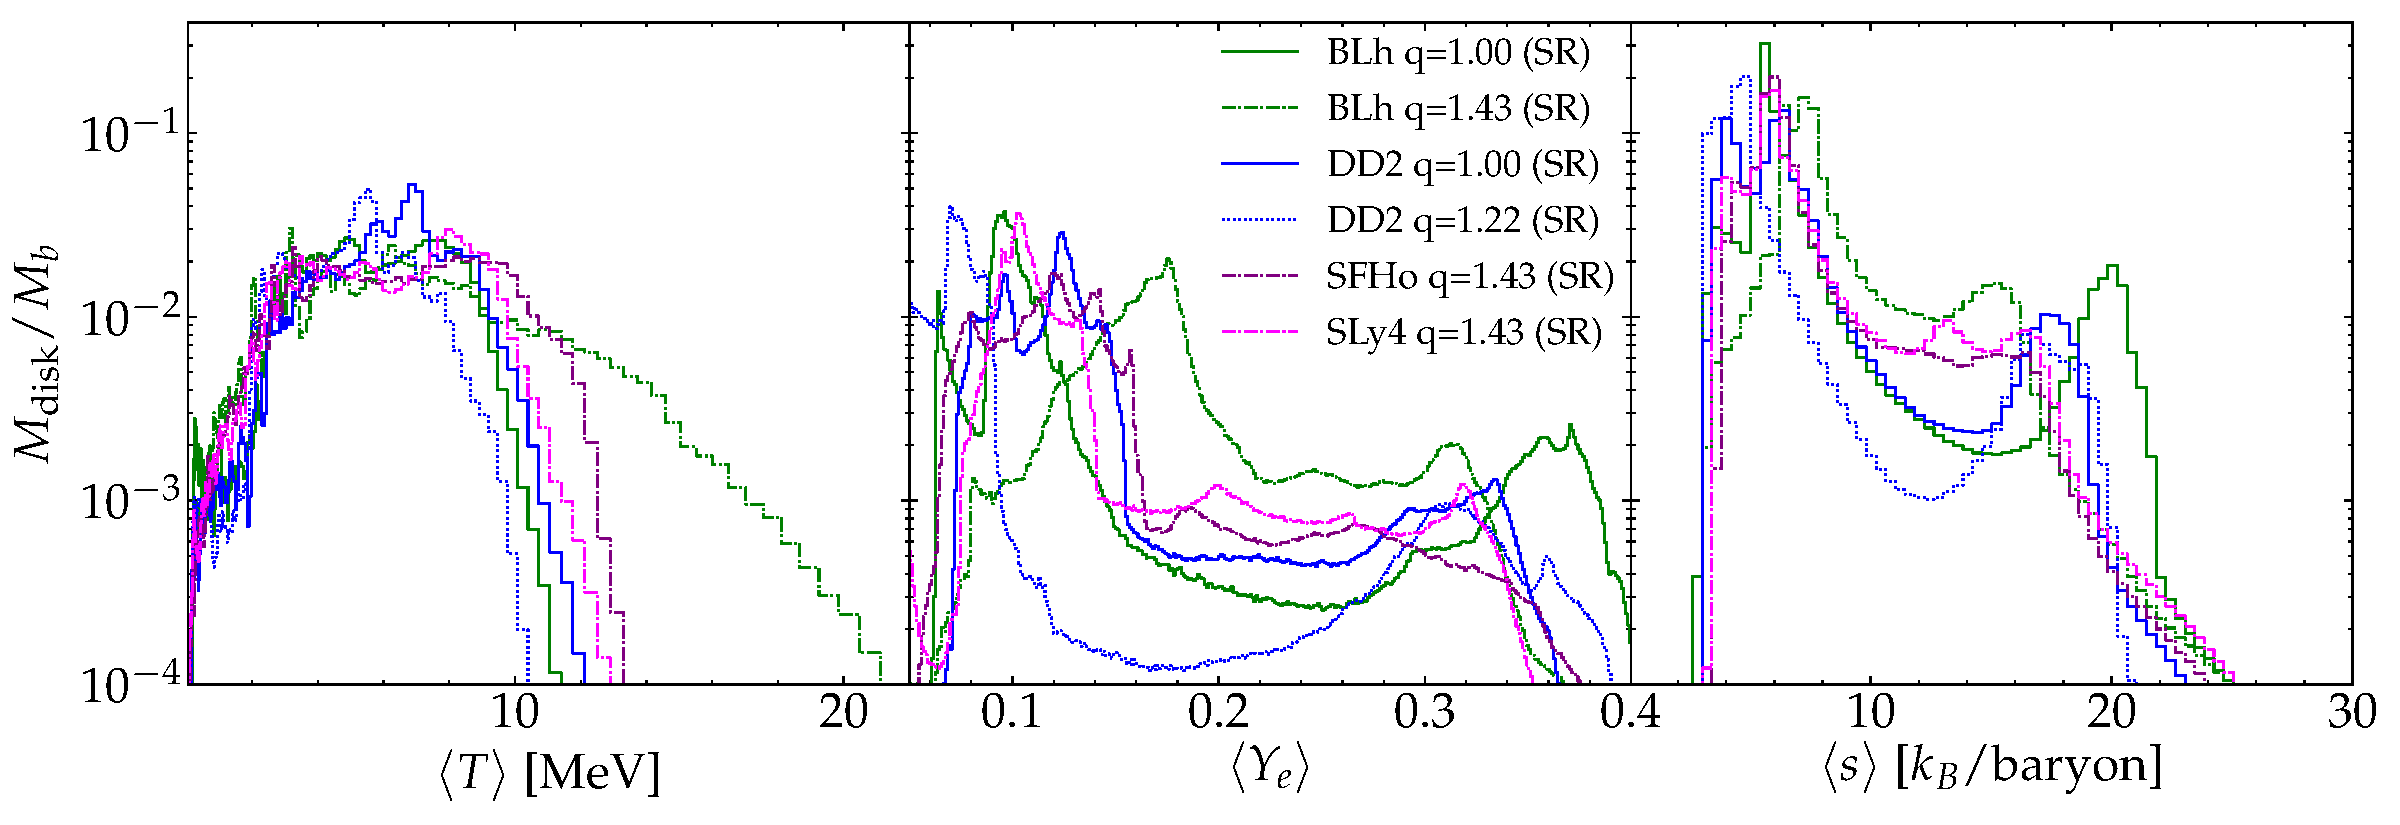
\includegraphics[width=0.95\textwidth]{disk/final_structure/disk_hist_shared.pdf}
    \caption{Composition of the disks at the end of the long-lived
        remnants simulations. The histograms refer to the temperature $T$
        (left),
        electron fraction $Y_e$
        (middle) and entropy $s$ (right).
        (Adapted from \citet{Nedora:2020pak})
    }
    \label{fig:final_disk_struct_hist_long}
\end{figure*}

In this section we discuss the final structure and properties of the disk, 
focusing on the models with long-lived \ac{MNS} remnants.
The properties are extracted at typical time $\sim60{-}100$~ms after merger.

We find that the generally the disk is optically thick.
The disk' RMS openning appears to be independent of the \ac{EOS} and \mr{} and
is $\langle\theta\rangle_{\text{rms}}\sim60^{\circ}$. 
The radial extend of the disk, however increases with the \ac{EOS} softness and 
binary \mr{}.
Similarly, the final disk mass is larger for the unequal mass binaries, 
ranging overall between ${\sim}0.1M_{\odot}$ and ${\sim}0.4M_{\odot}$
(see Tab.~\ref{tab:sim})..
Notably, for models with long-lived remnants the disk mass is larger,
that for the those with long-lived remnants. This can be attributed to the 
rapid accretion onto a \ac{BH} that removes $\sim50\%$ of the disk mass.
%% ---
We investigate the overall statistical properties of the disk mass for all our models
and those available in the literature in Sec.\ref{sec:results:Statistics:Mdisk}
\gray{
    The mean value of the disk mass in out models is 
    $\overline{M}_{\text{disk}}=(0.161 \pm 0.083)M_{\odot}$,
    where the standard deviation is also reported.
    %% ---
    Similarly to the dynamical ejecta we fit the disk masses with the 
    second order polynomial in $(q,\tilde{\Lambda})$.
    The coefficients of Eq.~\eqref{eq:fit:poly22}
    for this fit are given in Tab.~\ref{tab:fitpoly22coefs}.
    A more detailed study with various fitting formulas and extended
    datasets from the literature is reported in a companion paper.
}

Next, we consider the composition of the disk at the end of the simulation.
%% --- 
The mass-averaged temperature, electron fraction and entropy per baryon
are for several models are shown in Fig.~\ref{fig:final_disk_struct_hist_long}.
%% ---
We observe that the mass-weighted distribution of the entropy and electron 
fraction show a bimodal structure, which is more pronounced for the 
equal mass binaries. 
Regarding entropy, two peaks are present in the distribution:
a peak low entropy $s\sim5-10k_B/$baryon, that depends weakly of the 
\ac{EOS} and \mr{} and corresponds to the bulk, mildly shocked, material. 
The second peak is found at higher entropy, $s\sim15-22k_B/$baryon.
It corresponds fo the strongly shocked material and is more prominent 
in models with softer \ac{EOS}.
Notably, in the models with higher \mr{}, the second peak is located 
at lower $s$.
The mass-weighted distribution of the electron fraction 
displays a similar double-peak structure.
The low $Y_e$ peak that corresponds to the neutrino-shielded part of the 
disk is located around the $Y_e\sim0.1$.
The high $Y_e$ peak is located at $Y_e\sim0.3-0.4$ and corresponds to the outer parts of the disk, subjected to a strong neutrino irradiation.

In Fig.~\ref{fig:snapshots_xy_ye_entr} we show the electron fraction 
and entropy per baryon on the $xy$ and $xz$ slices of the equal 
mass model with BLh \ac{EOS}.
The plot shows, that the two peaks in the mass-weighted distribution 
of electron fraction and entropy correspond to different regions within the disk.

Overall, the most of the disk matter has temperature of $T\sim 1-10\,$MeV, with the innermost parts being hotter then the outer outermost. 
However, the disk temperature distribution appears to be largely independent of the \ac{EOS} and \mr{}

\red{Paragraph on the secular ejecta has been moved to 
    GW170817 application}


%% =======================================================
%%
%%                   Nucleosynthesis
%%
%% =======================================================

\todo{MAYBE another chapter with intro, method and results?}

\section{Nucleosynthesis}

\begin{figure*}[t]
    \centering 
    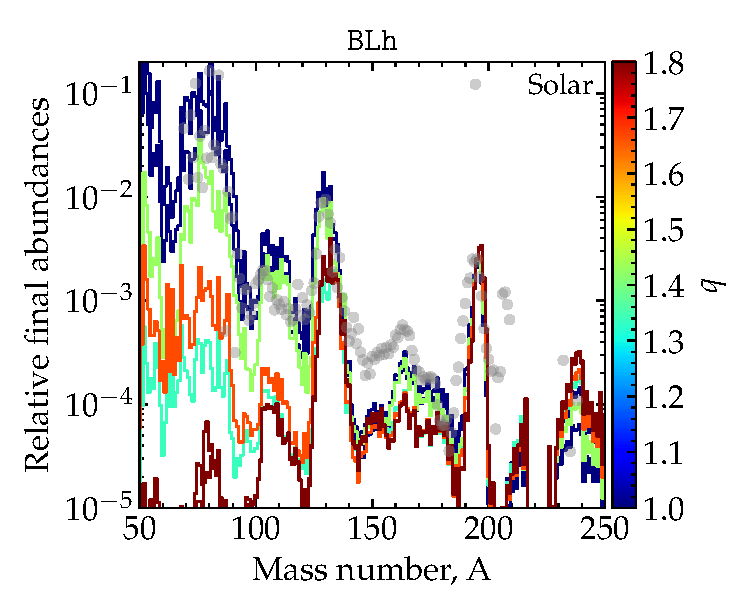
\includegraphics[width=0.45\textwidth]{nucleo/cc_nucleo_BLh_total.pdf}
    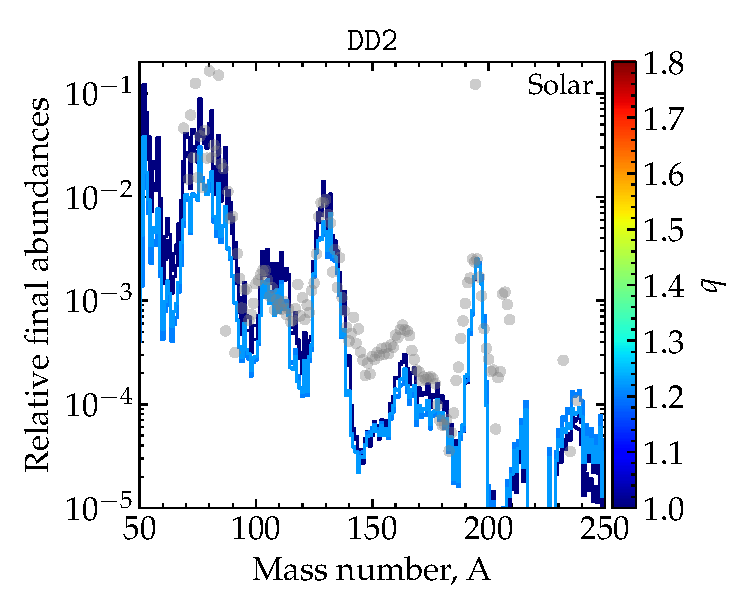
\includegraphics[width=0.45\textwidth]{nucleo/cc_nucleo_DD2_total.pdf}
    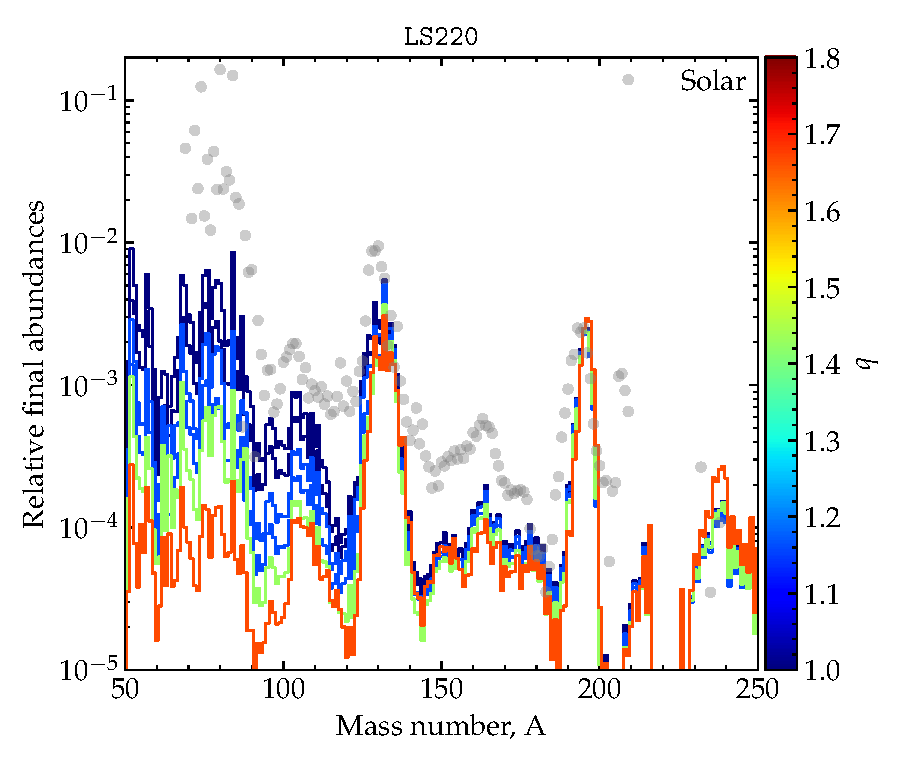
\includegraphics[width=0.45\textwidth]{nucleo/cc_nucleo_LS220_total.pdf}
    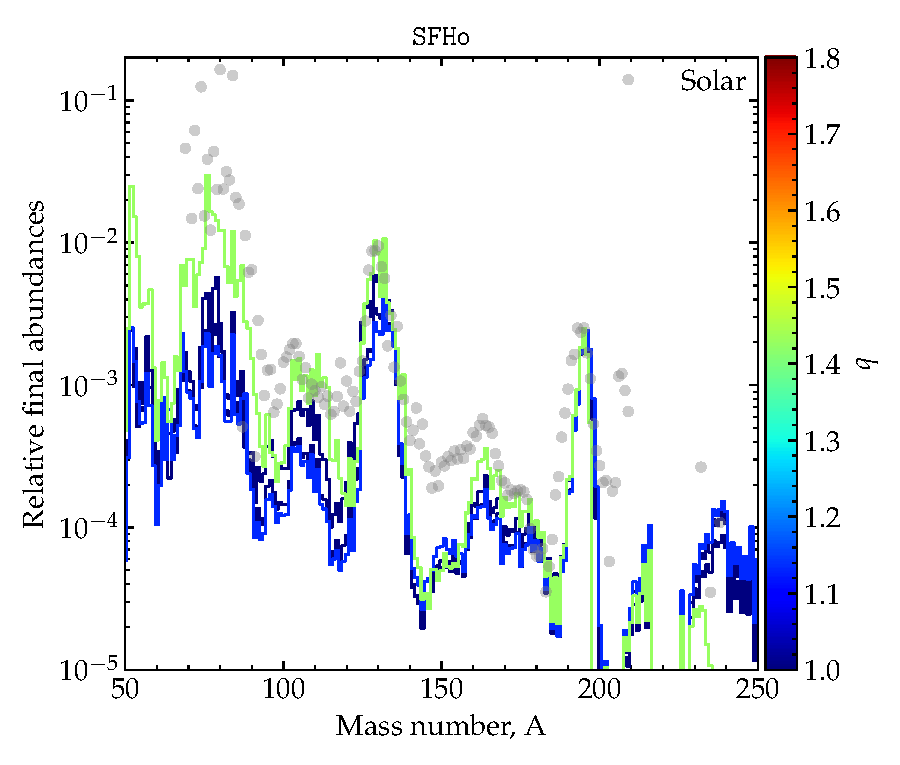
\includegraphics[width=0.45\textwidth]{nucleo/cc_nucleo_SFHo_total.pdf}
    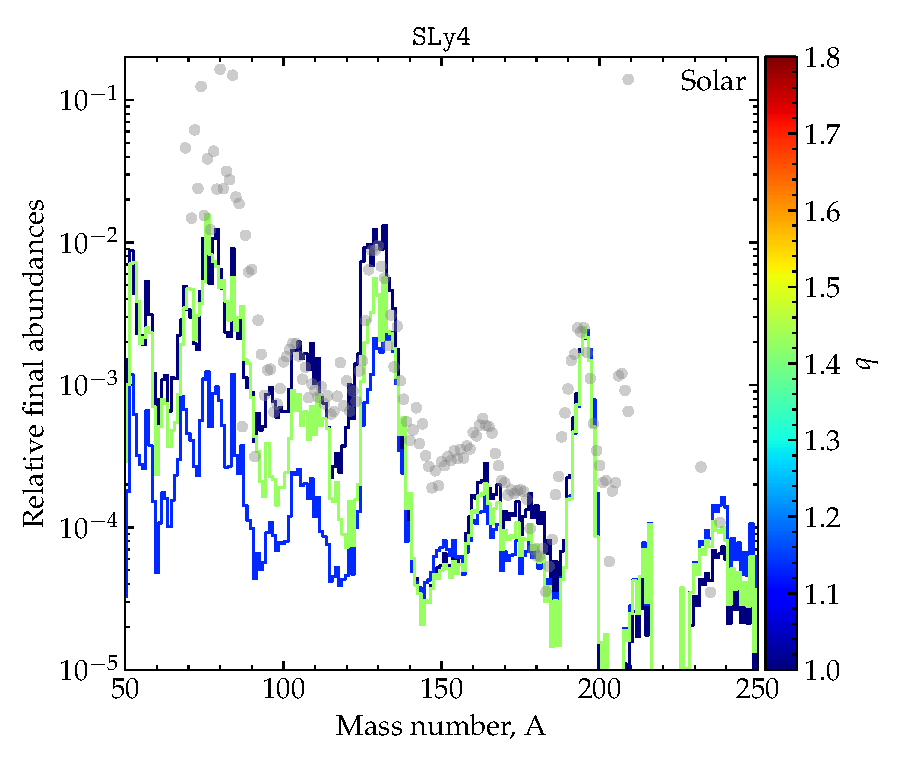
\includegraphics[width=0.45\textwidth]{nucleo/cc_nucleo_SLy4_total.pdf}
    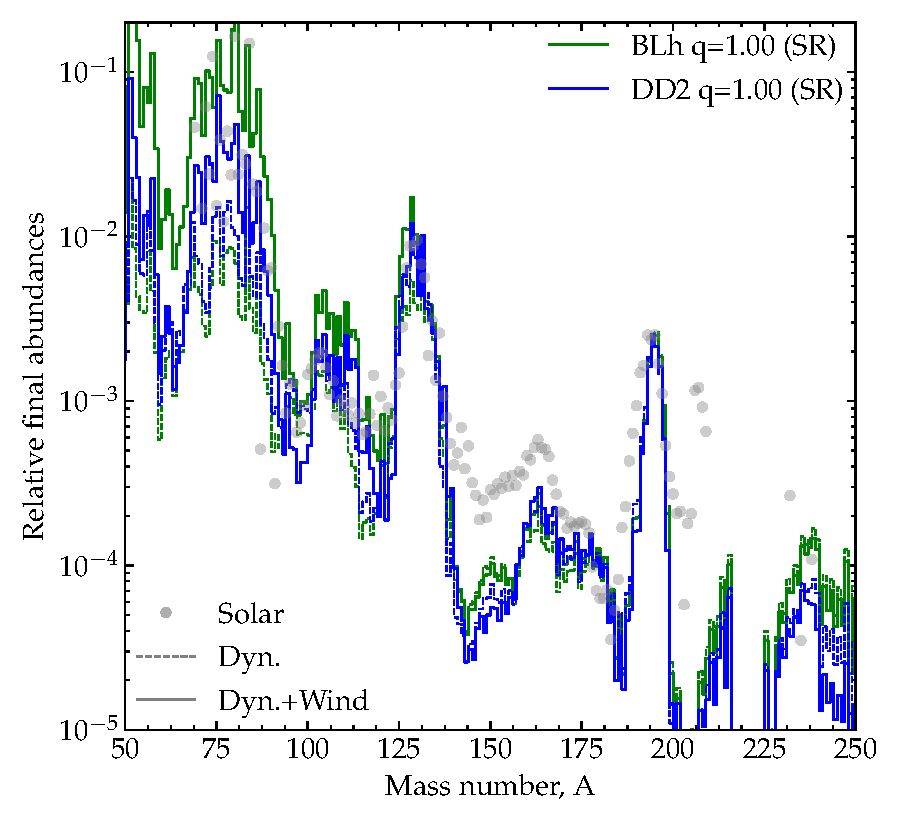
\includegraphics[width=0.42\textwidth]{nucleo/nucleo_dd2_blh.pdf}
    \caption{Nucleosynthesis yields for all simulations. Each %% panel
        of the first five panels 
        shows a different EOS and the scale color the dependency on the
        mass ratio. The nucleosynthesis is computed on the total ejecta
        computed during the simulations and 
        composed of the \ac{DE} (all models) plus the \ac{SWW} 
        (for the long-lived remnants listed in
        Tab.~\ref{tab:spiralwavewind}.).
        %
        The last (bottom-right) panel compares the nucleosynthesis in
        the \ac{DE} and \ac{SWW} for the long-lived
        remnants. The inclusion of the \ac{SWW} contributes to 
        improve the agreement with solar data for elements around the first peak.
        (Adapted from \citet{Nedora:2020pak})
    }
    \label{fig:nucle:totalyields}
\end{figure*}

The nucleosynthesis calculations are performed in postprocessing
following the same approach as in \cite{Radice:2016dwd,Radice:2018pdn}.

Here we briefly outline the procedure. 
Expanding ejecta undergoes the rapid neutrino capture nucleosynthesis, (\rproc{}).
In \citet{Lippuner:2015gwa} a new nuclear reaction network was presented 
(see Appendix~\ref{app:nuc} for more details). 
Using the parametrized \rproc{} calculations it is possible to map the ejecta 
parameters (discussed below) onto the final nucleosynthetic yields of our simulations.
The procedure is the following. 
For a given ejecta type (\eg, \ac{DE} or \ac{SWW}) we obtain the electron fraction,
entropy, velocity and rest mass density at a given extraction sphere 
(see Sec.\ref{sec:method:ejecta}).
The $r$-process in a given fluid element depends on how fast it decompresses from the 
merger environment (see Appendx~\ref{app:nuc}). 
This can be parametrized with the expansion timescale, $\tau$, assuming a specific 
velocity profile for the ejecta. We assume the homologous expansion \red{explain!}.
This assumption holds, as ejecta reaching the extraction sphere has already 
significantly decompressed and its density decreased ${\sim}3$~orders of magnitude. 
For the homologous expanding fluid, the density as a function of time reads 

\begin{equation}
\rho(t) = \rho_E\Big(\frac{\upsilon_E t}{r_E}\Big)^{-3} = 
\rho_E\Big(\frac{\upsilon_E t}{r_E}t\Big)^{-3},
\label{eq:nuc:rho_homolog}
\end{equation}

where $\rho_E$ and $\upsilon_E$ are the density and velocity of the fluid element 
when it crosses the radius $r_E$. 
%% ---
The density in the nucleosynthesis calculations has the profile \citep{Lippuner:2015gwa} 

\begin{equation}
\rho(t) = \rho(s, Y_e, T=6\text{GK})\Big(\frac{3\tau}{e t}\Big)^3
\label{eq:nuc:rho_nuccalc}
\end{equation}

where $e$ is the Euler's number, and $s$ and $Y_e$ are the fluid entropy and 
electron fraction.

Solving together Eq.~\eqref{eq:nuc:rho_homolog} and Eq.~\eqref{eq:nuc:rho_nuccalc},
the expansion timescale $\tau$ can be extracted.

In order to compute the nucleosynthetic yields we bin the ejecta in the 
parameter space of $(s, Y_e, \tau)$. 
%% --- 
Under the assumption of homologous expansion the \rproc{} outcome depends on 
the these quantities and can be precomputed.
%% ---
We compute the total nucleosynthetic yields by summing the contributions from 
each bin.

%% -------------------------------------

%However, part of the uncertainty lies in the yet insufficient understanding of the nucleosynthetic yields from the neutron star mergers. Here we study the $r-$process
%abundances from the mergers, focusing on the effect of mass-ratio and equation of state. Complimentary to the previous study \cite{Radice:2018pdn}, we include the post-dynamical ejecta, \textit{e.g.,} \swind, where the lifetime of the remnant is sufficiently long. \\
%
%For the nucleosynthesis calculations we employ the same approach as in \cite{Radice:2016dwd} and \cite{Radice:2018pdn} which we outline briefly. Consider the outflowing material, crossing the coordiante sphere surface with $R\approx294$km that satisfies the criteria to be unbound, (geodesic for the dynamical ejecta and Bernoulli for the \swind) the following properties. WE extract its electron fraction n $Y_{e,R}$, specific entropy $s_R$, velocity $\upsilon_R$ and the rest-mass density $\rho_{0,R}$. In addition, we assume that the following expansion of the material is homologous, \textit{i.e.,}
%
%\begin{equation}
%\rho_{0}(t) = \rho_{0,R}\Big(\frac{\upsilon_R}{cR}t\Big)^{-3}.
%\label{eq:nucleo:rho_t}
%\end{equation}
%
%Then we match the density decrease with radius, with the $\rho$ behavior available in the parameterized $r$-process calculations of \cite{Lippuner:2015gwa}
%
%\begin{equation}
%\rho_{0}(t) = \rho_{0}(s, Y_e, T=6\text{GK})\Big(\frac{3\tau}{et}\Big)^3,
%\label{eq:nucleo:rho_t_lipp}
%\end{equation}
%
%where $\tau$ is the expansion timescale, and $e$ is the constant $e\approxeq 2.718$. Matching the equations \ref{eq:nucleo:rho_t} and \ref{eq:nucleo:rho_t_lipp} yields $\tau$ as
%
%\begin{equation}
%\tau_d = \frac{eR}{3\upsilon_R}\Bigg(\frac{\rho_R}{\rho_0}\Bigg)^{1/3}.
%\end{equation}
%
%Nucleosynthesis network calculations allow for a homologous expansion  to precompute the yields as a function of $\{\rho_{0,R},s_R,Y_{e,R},\tau_R\}$. Binning the corresponding ejecta parameter space, we can then use this precomputed data to gauge the nucleosynthetic yields in every bin of ejecta. Summing them, we obtain the total yield. For the discussion of the uncertainty of this method, see \cite{Radice:2018pdn}. \\
%
%It is also worth noting other approaches to nucleosynthesis computations in ejecta. In principle, the method should involve tracking numerous isotopic abundances of the material, that is moving along the fluid flow, undergoing fission, mixing and spallation, accounting for the EOS dependent feedback to the underlying flow. This however would require modifications to the composition equation and would make models computationally very expensive. A simplification to this approach would be to ignore the backreaction of nucleosynthesis to the flow dynamics, following the composition changes of Lagrangian traces advocated by it. It is believed that fission, while producing entropy that alters the burning in non-trivial way, amounts to only marginally changing the flow dynamics of lightly bound material \vn{it is however interesting to see how this would change the \swind mass}. Thus, the tracer approach is reasonable approximation, that is widely used. The technical difference with respect to the arropach employed in this work, is that the density history $\rho(t)$ is tracked in the ejecta instead of the assumption of homologous expansion. The entropy $s_0$ and electron fraction $Y_{e,0}$ are extracted at the time $t_0$ and then evolved using a self-heating nuclear reaction network \cite{Freiburghaus:1999}. \\
%
%The comparison between tracer method and homologous expansion one is performed in \cite{Radice:2018pdn}. It was concluded that within a factor of two, methods yield similar results. However, several caveats were pointed out with respect to the errors arising in ignoring the actual density history ($25\%$). On the other had it was stated that due to the approximation of Eualian flow with Lagrangian the error of $\sim 40\%$ can be expected. \\
%
%Here, employing the homologous expansions method. We report the relative abundances of different isotopes synthesized by the $r$-process \red{32} years \vn{not sure where this number is set up} after the merger in the material ejected from the system. In the \textit{short-lived} cases this encompasses only the dynamical ejecta, while in the \textit{long-lived} ones (see table \ref{tab:wind}) it includes the \swind. As the electron fraction is the most important quantity determining the outcome of the $r$-process \cite{Lippuner:2015gwa,Radice:2016dwd}, we report it for selected \textit{long-lived} models in figure \ref{fig:ejecta:bern:hist}. In the figure \ref{fig:nucleo:dynvswind} we compare how the inclusion of the \swind changes the abundances of two representative models and in the figures \ref{fig:nucleo:dynonly} and \ref{fig:nucleo:dynvswind} we show the total abundances of a large  subset of models, investigating the effect of mass ration and EOS (without and with the inclusion of \swind respectively). In all cases, we compare our abundances with the up-to-date solar ones from \cite{Prantzos2020} (for a review of the solar system abundances see \textit{e.g.,} \cite{Pritychenko:2019xvf}). The latter are normalized to the sum of all elements, while the model abundances are normalized to the solar at $A=195$. This is justified as long as ejecta contains very neutron rich material, as the nuclear fission cycling leads to a robust profile that follows the third $r$-process peak \cite{Lippuner:2015gwa}.\\
%
%The \cite{Radice:2018pdn} presents the systematics of the nucleosynthetic yields of a large subset of models, for which neutrino re-absorption has been neglected. Here we extent this by performing a similar analysis albeit with the subset of models that include the neutrino re-absorption. In addition, the subgrid turbulence is included in most of our models. However, its effect is much weaker then the one of the mass-ratio. Indeed, the figure \ref{fig:nucleo:dynonly} shows a model's ability to reproduce the solar $1$st and $2$nd r-process peaks, at $A\sim 100$ and $A\sim 125$ respectively strongly depended on the mass-ratio. Higher $q$ models, whose dynamical ejecta is mostly of tidal tail origin with very low electron fraction show severe underproduction of light $r$-process material, while $q=1$ DD2 and BLh models are able to reproduce both peaks reasonably well. This is the result of inclusion of neutrino reabsortion as it increases the $Y_e$ of the shocked component of the ejecta \cite{Radice:2018pdn}. Note, however, that in \cite{Papenfort:2018bjk} the effect of $q$ was not found. But similar to both studies, with respect to the equation of state, we do not observe consistent changes between still anf soft ones. This has also been the case in the aforementioned study.\\
%
%Important to note the actinides production, elements with atomic number $A\sim 230$. It was previously reported that in binary neutron star merger ejecta these materiel is overproduced (see \textit{e.g.,} \cite{Giuliani:2019oot}). However, we hint that this conclusion might partially be motivated by a choice of normalization. If we employ the physically motivated normalization to $A = 195$ of solar abundances, we observe that the actinides abundances are consistent with solar. We also note that there is dependency on the mass-ratio, motivated once again, by the ejecta composition. The very low $Y_e$ of highly assymetric models leads to significant boost in actinides production. This is the case for $q=1.8$ of BLh and $q=1.67$ of LS220. \\
%
%Indeed, to explain the $^{232}$Th solar abundances the average electron fraction in the ejecta should lower and any of our models except promptly collapsing ones can achieve. This underlines the importance of such mergers for $r$-process nucleosynthesis. We however emphases, that with adopted in this work normalisation, we do not observe overproduction of actinides, that was reported in \cite{Holmbeck:2019xnd}. \\
%
%+
%In the \textit{long-lived} case, the dynamical ejecta amounts to a small fraction of the total mass of material leaving the system. The second, more massive component, is the \swind. Its overall high electron fraction (see Fig. \ref{fig:ejecta:bern:hist}) implies that the weak $r$-process is dominant one here and light elements $A<195$ are primarily produced. In figure \ref{fig:nucleo:dynvswind} we compare the relative abundances from nucleosynthesis in dynamical ejecta only, with the total ones. Owing to the normalization to the $3$rd peak, it is reproduced in both cases, and the important difference lies in the $1$st and $2$nd peaks. In case of BLh we see that solar abundances of even very light elements $A\sim75$ are robustly reproduced. However there is an overproduction of $A\sim 110$ and $A\sim 130$ elements. The DD2 model, on the other hand, shows an overall lower total abundances. This is attributed to the slightly lower average electron fraction in DD2 (Fig. \ref{fig:ejecta:bern:hist}) while the ejecta masses are very similar (Fig.\ref{fig:mej:bern}). \\
%
%In the figure \ref{fig:nucle:totalyields} we investigate the total mass-ratio dependence of the total abundances. It is important to emphasis that in \textit{short-lived} cases this is the abundances of the dynamical ejecta only. Thus we limit this discussion to the DD2 and BLh models, most of which are sufficiently long with only extreme high $q$ BLh ones being an exception. Notably, the abundances strong $q$ dependence observed in dynamical ejecta, is not present for total ejecta, and all the $r$-process peaks are reasonably well reproduced by all the \textit{long-lived} models. This is not too surprising owing to the robust properties of the \swind, that change only marginally between different models. \\
%
%Overall, we find that dynamical ejecta of asymmetric models in general underproduces the $1$st and $2$nd r-process peaks due to its low average electron fraction. Equal mass DD2 and BLh models however are able to reproduce these peaks. Meanwhile, the total ejecta of DD2 and $q<1.7$ BLh models reproduces both, $1$st and $2$nd r-process peaks reasonably well irrespective of the mass-ratio, showing that the complete solar $r$-process abundances can be recovered if the remnant is \textit{long-lived}. This further supports the hypothesis, that binary netuton stars are the prime source of $r$-process material in the Universe.\\
%
%It is however, important to note that nucleosynthetic yields are subjected to the choice of nuclear input data. In particular, the choice of fission fragment distributions and neutron induced fission rates may have a large impact on abundances in the region of the $1$st and $2$nd peaks \cite{Eichler:2014kma}. The symmetric fission fragment distributions used in our calculations does most likely underproduce material in this region. In addition, as the neutrino-matter interaction rates roughly scale with the square of the incoming neutrino energy. Thus, the nucleosynthetic yields depend on the details of the neutrino radiation spectra \cite{Foucart:2016rxm}. The energy integrated scheme, employed in this work, does not allow us to take this effect into account (see, however, \cite{Radice:2018pdn} where different neutrino energy distributions were studied). It was recently pointed out that the neutrino resonant oscillations and fast flavor conversion might occur in NS merger remnants \cite{Zhu:2016mwa,Frensel:2016fge,Deaton:2018ser}. This might modify the nucleosynthesis of light $r$-process elements \cite{Wu:2016pnw}. Thus there is a need for more sophisticated simulations with spectral neutrino transport taking into account the neutrino oscillations. \\
%
%In addition to the dynamical ejecta and \swind, the $r$-process nucleosynthesis occurs in the secular ejecta. In particular in neutrino-driven winds, where neutrino irradiation of the expanding ejecta considerably increases the electron fraction. If the velocity of the ejecta sufficiently low, the material achieves $Y_e$ given by the weak equilibrium in optically thin conditions with neutrinos \cite{Qian:1996xt}. During the early post merger phase this $(Y_e)_{eq}\leq 0.45$ which allows for a weak $r$-process nucleosynthesis of light elements $A<130$ to occur \cite{Dessart:2008zd,Perego:2014fma,Foucart:2016rxm,Martin:2015hxa}. In addition, is expected that the dominant source of ejecta from the merger is the viscously-driven outflow from massive disk, if it forms after the merger. Properties on such outflow has been recently investigated in a framework of axisymmetric BH-torus systems \cite{Fernandez:2013tya,Just:2015fda}. The $Y_e$ distribution was found to be broad allowing all $r$-process elements from the $1$st to the $3$rd peak, as well actinides, to be synthesized in proportions close to solar (\textit{e.g.,} \cite{Wu:2016pnw}). If the \textit{long-lived} remnant is present however, the properties of the viscous ejecta are expected to be significantly altered by the large amount of neutrinos emitted over the diffusion time scale (seconds, \textit{e.g.,} \cite{Dessart:2008zd,Perego:2017fho}). 



%% -------------------------------------



\red{Radice:2018pdn disussion on the accuracy/}.

\red{Something to check}
\gray{
    We do not nd material with expansion timescale of
    less than 0:5 ms. This seems to exclude the neutron freezeout
    scenario proposed by Metzger et al. (2015). However,
    the lack of a very fast component of the ejecta might also
    be due to numerical effects. Our resolution is probably not
    high enough to track the very small fraction of the ejecta
    expected to experience neutron freeze-out in the scenario
    proposed by Metzger et al. (2015).
}


%% ----------- results ----------------- 

With the procedure outlined above we compute the isotopic abundances of 
the \rproc{} elements $32$~years after merger. 
%% ---
The novelty of the results presented in this section is in the more 
advanced neutrino treatment, as all out models include the effects of neutrino 
self absorption (in comparison with \citet{Radice:2018pdn}), the inclusion 
of the \ac{SWW}, and models with high \mr{}, $q\geq1.8$. 
%% ---

In the Fig.~\ref{fig:nucle:totalyields} (except the bottom right panel), 
we show the nucleosynthesis yields from overall ejecta with each panel 
containing all models fro a given \ac{EOS}, with the \mr{} being color-coded.
For models with short-lived \ac{MNS} remnants the total ejecta is compised 
of the \ac{DE} only, while for models with long-lived ones, the total ejeta 
consists of \ac{DE} and \ac{SWW}. 
%% --- 
We compare the model abundances with the recently updated solar residual 
\rproc{} abundances from \citet{Prantzos2020} 
(for a review of the solar system abundances see \eg~\citealt{Pritychenko:2019xvf}).
For the qualitative comparison between models and observations we employ 
the following normalization. 
The model abundances are multiples by a constant factor that makes the abundances at 
$A=195$ equal solar.
%% --- 
From the plot we observe that final \rproc{} abundances in the ejecta from models that 
form long-lived \ac{MNS} remnants with DD2 and BLh \acp{EOS}, are in a greement with 
solar across all three \rproc{} peaks. 
\red{add some info on peaks themselves.}
Due its robust properties, the \ac{SWW} allows for the complete reproduction 
of the solar \rproc{} abundances. 
\red{A note on the high Ye and light element productioN?}
%% --- 
With respect to the models with short-lived remnants, the final \rproc{} eject abundances 
at solar $1$st and $2$nd \rproc{} peaks, (at $A\sim 75$ and $A\sim 125$ respectively) 
depend strongly on \mr{}. 
For instance, models with high \mr{} have \ac{DE} of tidal origin mostly with low 
electron fraction. The final \rproc{} abundances in this ejecta show the underproduction 
of light elements. 
The final abundances in ejecta from equal mass binaries, 
however, shows that even light \rproc{} elements are 
synthesized. This is because the neutrino reabsorption raises the electron fraction 
in the shocked component of the \ac{DE} \citep{Wanajo:2014wha,Radice:2018pdn}. 

%% --- 
We observed that final abundances in the ejecta in all our models show the 
presence of actinides, elements with $A\sim230$. 
The amount of actinides produced, however, depends strongly on the ejecta 
electron fraction, and thus, on the binary \mr{}.
The agreement with solar abundances is found only for very asymmetric binaries. 
Notably, that only for the binaries with the highest \mr{}, $q\sim1.8$, the 
\rproc{} in the \ac{DE} results in both $3$rd peak and actinides(at $^{232}$Th) abundances 
close to solar values. 
This suggests that the high \mr{} mergers or \ac{NSBH} mergers might be an 
important contributor to the cosmic chemical evolution.

%%--- Bottom right panel
The total ejecta from the models with long-lived \ac{MNS} remnants is dominated by
the \ac{SWW}, as its mass is generally limited by the \ac{MNS} lifetime 
or by the evolved time (Sec.~\ref{sec:results:ejecta:sww})
In the bottom-right panel of Fig.~\ref{fig:nucle:totalyields} we show separately the 
final abundances from the \rproc{} in the \ac{DE} and in the \ac{DE} plus \ac{SWW}. 
The electron fraction of the \ac{SWW} is higher than that of the \ac{DE} 
(see Fig. \ref{fig:ejecta:bern:hist}), and this the \rproc{} nucleosynthesis in the 
\ac{SWW} produces primarily light elements around the first \rproc{} peak, $A<95$.
We recall here, that due to the choice of the normalization, all abundances are up-scaled 
to reproduce the $A=195$ peak. We asses here the relative abundances at $1$st and $2$nd
\rproc{} peaks.
%% ---
The plot shows that for the BLh models the amount of lighter elements, $A\sim75$, is higher with 
respect to the DD2 model. This can be attributed to the higher electron fraction in the 
\ac{SWW} of the former (see Fig. \ref{fig:ejecta:bern:hist}).
In both cases, however, the abundances of light elements are very close to slolar 
\red{can be extended by adding plot from the Letter}

%% --- other ejecta types
The \rproc{} is expected to take place in other types of ejecta from \ac{BNS} mergers.
In \nwind{} the neutrino irradiation raises the electron fraction, that, depending 
on the ejecta velocity, can reach the $Y_e\leq 0.45$ \citep{Qian:1996xt}. 
At this pint the weak equilibrium sets in between the ejecta and neutrinos.
High electron fraction implies that only the light elements will be produced.
The numerical studies indeed support this picture 
\citep{Dessart:2008zd,Perego:2014fma,Just:2014fka,Martin:2015hxa,Foucart:2016rxm}. 
%% ---
The bulk of the ejecta from \ac{BNS} mergers is expected to come in the form of 
viscous- and recombination-driven winds, This ejecta, however, is expected to take 
place over the longer timescales than those of our simulations.
Studies have shown that this ejecta has a broad distribution of the electron fraction 
and the \rproc{} nucleosynthesis within it would produce light as well as heavy elements
\citep{Fernandez:2013tya,Just:2014fka,Wu:2016pnw,Siegel:2017nub,Fujibayashi:2017puw,Fernandez:2018kax}.
The production of the heavy \rproc{} elements, however, might be supressed in this winds
if the long-lived \ac{MNS} is present \citep{Metzger:2014ila,Lippuner:2017bfm}.


%% =======================================================
%%
%%                   Conclusion
%%
%% =======================================================

%% ========================================================================================

\section{Statistics of the \ac{DE} parameters and disk mass}

\red{CONTENT OF THE FIT PAPER}


\section{Application to \GW{}}


\begin{figure*}[t]
    \centering 
    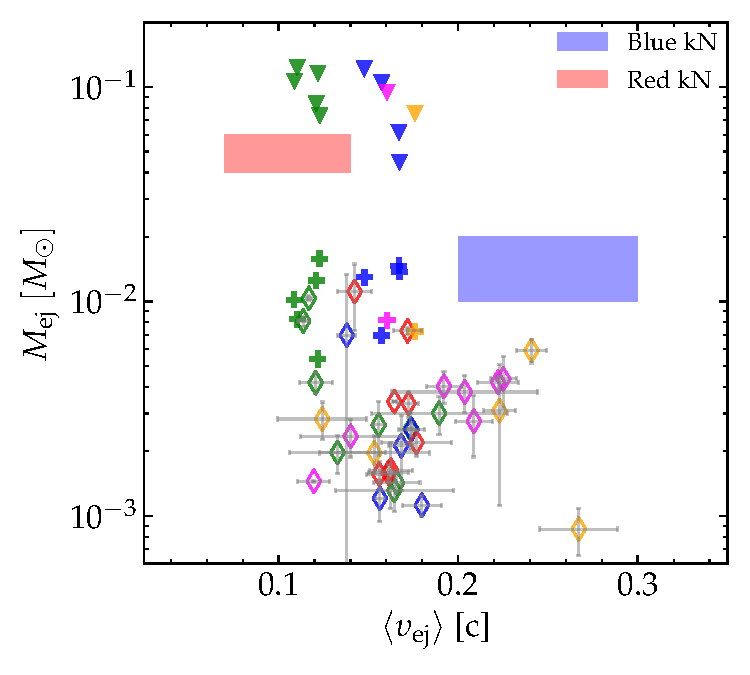
\includegraphics[width=0.48\textwidth]{ejecta_dyn/summary/ej_mej_vej_our2.pdf}
    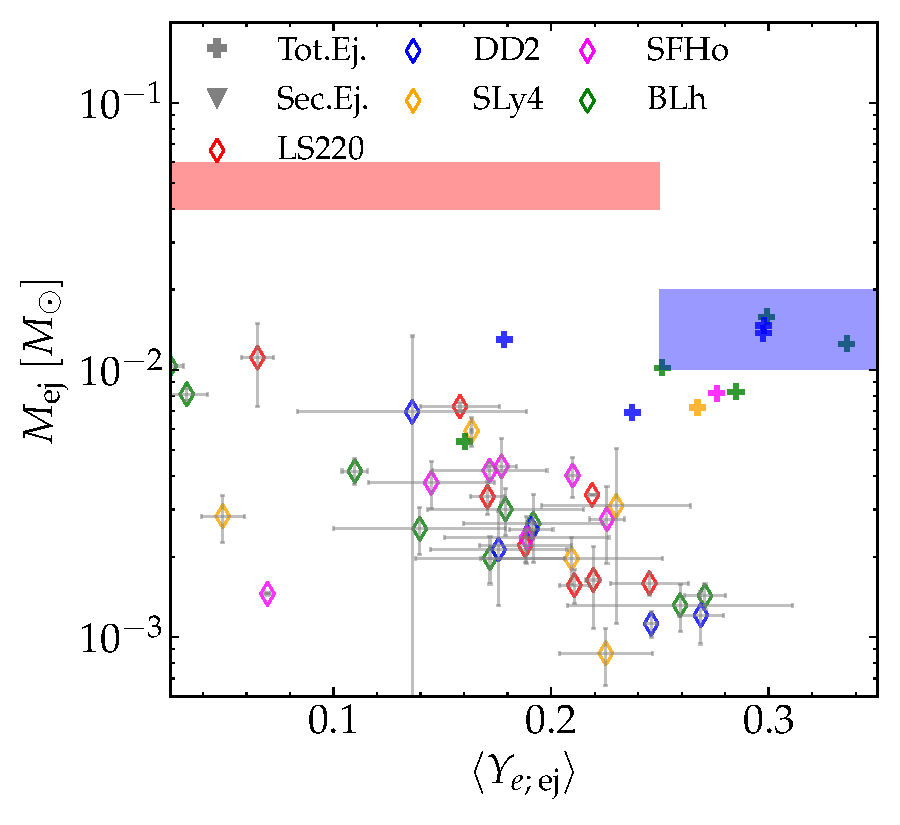
\includegraphics[width=0.48\textwidth]{ejecta_dyn/summary/ej_mej_yeej_our2.pdf}
    \caption{
        Summary of the ejecta properties of our models.
        %
        Diamonds mark the dynamical ejecta, crosses include the
        contribution of the \swind{} for the long-lived models, 
        triangles are an estimate of the total ejecta mass on a secular
        timescale, assuming $40\%$ of the disk mass is unbounded on
        secular timescales.         
        The ejecta mass is shown is terms of the mass-averaged velocity
        (left) and of the averaged electron fraction (right).
        %
        The filled blue and red patches are the expected values of
        ejecta mass and velocity for blue and red components of
        AT2017gfo compiled by \cite{Siegel:2019mlp}, based on
        \cite{Villar:2017wcc}. 
        Adopted from \citet{Nedora:2020pak}.
    }
    %
    \label{fig:ejecta:dyn:ds_sww}
\end{figure*}


%% from main paper, referencing the fitpaper Poly22 fits and SWW + DE
\red{THis can be augmented with Radio afterglow}

%% === FROM DYNAMICAL EJECTA SECTION of MAIN PAPER
Here we discuss the application of our results to \GW{}.


\subsection{Dynamical Ejecta}


%% ---
First, we asses the ejecta parameters that our fitting models, 
obtained in section \ref{sec:ejecta_disk_statisitcs} would provide for the \GW{}.
%% --- 
Considering the $90\%$ credible intervals estimated for $q$ and $\tilde{\Lambda}$ 
from LIGO-Virgo GW analysis
\citep{TheLIGOScientific:2017qsa,Abbott:2018wiz,De:2018uhw,Abbott:2018exr},
i.e.~$\tilde{\Lambda}=300_{-190}^{+500}$ and $q\in[1., 1.37]$. 
and using the errorbars formulas developed in \cite{Radice:2018pdn}, we find that
$\amd \in [0.72, 7.52] \times 10^{-3}\: M_{\odot}$
and
$\avd \in [0.16, 0.39]$c 
and 
$\ayd \in [0.11, 0.23]$.
Notably, these values do not agree with those inferred for \AT{} by the spherical, 
two-component kilonova models \citep{Villar:2017wcc}.
Analysis of a compiled set of kilonova fitting models provides a broad range of ejecta 
parameters \citep{Siegel:2019mlp}:
$M_{\text{ej}}^{\text{red}}\in(4, 6)\times10^{-2}M_{\odot}$ and
$\upsilon_{\text{ej}}^{\text{red}}\in(0.07, 0.14)$ for the red component, while
$M_{\text{ej}}^{\text{blue}}\in[1, 2]\times10^{-2}M_{\odot}$ and 
$\upsilon_{\text{ej}}^{\text{blue}}\in[0.2, 0.3]$ for the blue component.
%% ---
With respect to our results for \ac{DE}, however, 
none of the kilonova components can be well explained.
%% ---
In Fig.~\ref{fig:ejecta:dyn:ds_sww} we show the ejecta properties from
all our models (diamonds) and the parameters inferred from the
observations as red and blue boxes. 
%% --- 
With respect to the red component, we observe that \ac{DE} from our models 
have too high average velocities and not nearly enough mass.
This result suggests that an additional, low $Y_e$ ejecta component is required
in order to explain the \AT{} red component 
\citep{Perego:2017wtu,Kawaguchi:2018ptg,Nedora:2019jhl}.
%% --- 
A more thorough analysis of the \AT{} with better ejecta models and advanced
radiation transport kilonova simulations are not part of the present work 
and will be addressed in the future.


\subsection{\swind{}}


The \ac{SWW} could be a significant contributor to the \AT{}, assuming the remnant of 
\GW{} \ac{MNS} merger survived for $\mathcal{O}(100)$~ms.
%% ---- 
In Fig.~\ref{fig:ejecta:dyn:ds_sww} we report the total
(dynamical+\swind{}) ejecta mass and mass-averaged velocity for the
simulated long-lived BNS (crosses).
%% ---
Notably, the total ejecta mass of three of our models, 
BLh $q=1.18$, BLh $q=1.42$ and  DD2 is $q=1$ are in agreemnt with the epected values 
for the blue compoent of the \AT{} 
(obtained using the two-component fit \citep{Villar:2017wcc})

\red{
    [ LETTER STUFF COULD GO HERE ]
    a multi-component fitting model that explicitly accounts
    for the \swind{} can fit the early blue
    emission from AT2017gfo \citep{Nedora:2019jhl}
}

The high electron fraction of the \ac{SWW} however would result in a lanthanides-poor
composition of the outflow. Thus, the \ac{SWW} cannot explain the observed emission 
for the high opacity, lanthanides-rich material.
%% ---
Simulations with advanced physics of a \ac{MNS} mergers on a timescales $>100$~ms are 
required to asses the contribution from other outflow mechanisms, \red{that we will discuss below} 
\citep{Lee:2009uc,Fernandez:2015use,Siegel:2017nub,Fujibayashi:2017puw,Fernandez:2018kax,Radice:2018xqa}.


\subsection{Secular Ejecta}


On the timescale of seconds, much longer than the evolution of 
presented here simulations, the nuclear recombination can unbind 
a fraction of the disk mass. 
Analytical estimates and simulations with various approximations show that up tp ${\sim}40\%$ of the disk can be ejected via viscous processes with an typical velocity ${\lesssim}0.1\,$c
\citep{Lee:2009uc,Fernandez:2015use,Wu:2016pnw,Siegel:2017nub,Fujibayashi:2017puw,Fernandez:2018kax,Radice:2018xqa,Fujibayashi:2020dvr}.

Adapting the fix fraction of the $40\%$ of the disk mass, we estimate 
that about  ${\sim}0.05\, M_{\odot}$ would be ejected in a form of 
secular winds. We include this estimate for every simulation
with the long-lived \ac{MNS} remnant in Fig.~\ref{fig:ejecta:dyn:ds_sww} (lower triangles).
The estimated mass is sufficient to explain
the red component of AT2017gfo, as inferred from the two-components kN
models of \cite{Villar:2017wcc}. 







%% ---------------------
Sources with time delay are preferred by studies of very metal poor stars that indluded the time delay for r-process elements
to diffuse through ISM, \citep{Tarumi:2021xvw}. 
A winds from proto-nuetron are also contributors to the $r$-process budget \cite{Vincenzo:2021rvw}

\red{The remnant is losing anular momentum while disk gains on shortly after merger is due to gravitational torque \cite{Shibata:2019wef}}
 
%\include{Chapters/Chapter5} 


%----------------------------------------------------------------------------------------
%	THESIS CONTENT - APPENDICES
%----------------------------------------------------------------------------------------

\appendix % Cue to tell LaTeX that the following "chapters" are Appendices

% Include the appendices of the thesis as separate files from the Appendices folder
% Uncomment the lines as you write the Appendices
%%% ============================
%%
%% Appendix A
%%
%% ============================

\chapter{Derivation of Eistein field equations}
\label{app:efe}
%% \externaldocument{intro}
%% --------------------------------------


\section{Euler-Lagrange equations}

The action principle of the Lagrangian field theory on the spacetime $(\mathcal{M}; \boldsymbol{g})$ is
\begin{equation}
S(\boldsymbol{q}, \nabla\boldsymbol{q}) = \int_{\mathcal{M}}\boldsymbol{\alpha}\mathcal{L}(\boldsymbol{q}, \nabla\boldsymbol{q}),
\end{equation}
where $\boldsymbol{q}$ are a set of generalized coordinates for the fields described by the theory, $\nabla$ is the Levi-Civita connection, $\mathcal{L}$ is a scalar density of a scalar quantity $\lambda$ as $\lambda(\boldsymbol{q},\nabla\boldsymbol{q})$. 

Varying the action with respect to the $\boldsymbol{q}$
\begin{equation}
\delta S(\boldsymbol{q}, \nabla\boldsymbol{q}) = \delta\int\boldsymbol{\alpha}\mathcal{L}(\boldsymbol{q}, \nabla\boldsymbol{q}) = \int\boldsymbol{\alpha}\Big(\frac{\partial\mathcal{L}}{\partial\boldsymbol{q}}\delta\boldsymbol{q}+\frac{\partial\mathcal{L}}{\partial(\nabla\boldsymbol{q})}\delta\nabla\boldsymbol{q}\Big)
\end{equation}

As $\delta$ and $\nabla$ commute, and partially integrating $\nabla$, we obtain

\begin{equation}
\partial S(\boldsymbol{q}, \nabla\boldsymbol{q}) = \int\boldsymbol{\alpha}\Big(\frac{\mathcal{L}}{\partial\boldsymbol{q}}-\nabla\frac{\partial \mathcal{L}}{\partial(\nabla\boldsymbol{q})}\Big)\delta\boldsymbol{q} + \int_{\mathcal{M}}\boldsymbol{\alpha}\nabla\Big(\frac{\partial\mathcal{L}}{\partial(\nabla\boldsymbol{q})}\delta\boldsymbol{q}\Big)
\end{equation}

The last term is a boundary term and in order to vanish we impose boundary condition. Assume that the fields are defined over only a compact domain. \\
As the choice of $\partial\boldsymbol{q}$ is arbitrary, the 

\begin{equation}
\partial S(\boldsymbol{q}, \nabla\boldsymbol{q}) = 0
\end{equation}

and the Euler-Lagrange equations are

\begin{equation}
\frac{\partial \mathcal{L}}{\partial\boldsymbol{q}} - \nabla\Big(\frac{\partial\mathcal{L}}{\partial(\nabla\boldsymbol{q})}\Big) = 0
\label{eq:theory:eulerlagrange}
\end{equation}

%% ----------------------------------------------- 
\section{The Hilbert Action}

The Einstein–Hilbert action allows to obtain an Einstein field equations through ad principle of least action. Here we briefly underline the procedure.

Introduce action that describes the graviatational field, and a matter field $\mathcal{L}_m$:
\begin{align}
S_g &= \int\frac{1}{2\kappa}R\epsilon, \\
S_m &= \int\mathcal{L}_{m}\epsilon,
\end{align}
where $R$ is the Ricci scalar and $\kappa$ is the  Einstein's constant. \\

The full action then:
\begin{equation}
S = \int\Big(\frac{1}{2\kappa}R+\mathcal{L}_m\Big)\epsilon
\end{equation}

The action principle dicatates, that $\delta S = 0$  with respect to the inverse metric $g^{\mu\nu}$. 

\begin{equation}
\int\Bigg[\frac{1}{2\kappa}\Big(\frac{\delta R}{\delta g^{\mu\nu}}+\frac{R}{\sqrt{-g}}\frac{\delta\sqrt{-g}}{\delta g^{\mu\nu}}\Big) + \frac{1}{\sqrt{-g}}\frac{\delta(\sqrt{-g}\mathcal{L}_m)}{\delta g^{\mu\nu}}\Bigg]\delta g^{\mu\nu}\epsilon
\end{equation}

Owing to the arbitrariness of $\delta g^{\mu\nu}$, the integrant must be zero. 

\begin{equation}
\frac{\delta R}{\delta g^{\mu\nu}} + \frac{R}{\sqrt{-g}}\frac{\delta\sqrt{-g}}{\delta g^{\mu\nu}} = -2\kappa\frac{1}{\sqrt{-g}}\frac{\delta(\sqrt{-g}\mathcal{L}_m)}{\delta g^{\mu\nu}} = -\frac{2\kappa}{\sqrt{-g}}\frac{\delta S_m}{\delta g_{\mu\nu}} := \kappa T_{\mu\nu},
\label{eq:theory:action1}
\end{equation}
where we introduced the stress-energy tensor $T_{\mu\nu}$ and te matter action $S_m$ for future use. \\

\todo{this matter action is used in deriving the $T_{\mu} ^{\nu}$ i the invariant fluid formalisn}

The continuation of this deriviation requires taking variation of the Riccia scalar $R$ and the determinantof the metric $\sqrt{-g}$. As this is a length procedure, we provide here the result. 

\begin{equation}
\frac{\delta R}{\delta g^{\mu\nu}} = R_{\mu\nu},
\label{eq:theory:deltaR}
\end{equation}
where the $R_{\mu\nu}$ is the Ricci curvature tensor.

\begin{equation}
\frac{1}{\sqrt{-g}}\frac{\delta\sqrt{-g}}{\delta g^{\mu\nu}} = -\frac{1}{2}g_{\mu\nu}.
\label{eq:theory:deltagmuny}
\end{equation}

Substituting Eq. \ref{eq:theory:deltaR} and Eq. \ref{eq:theory:deltagmuny} into equation of motion Eq.  \ref{eq:theory:action1} we obtain the Einstein's field equation 

\begin{equation}
R_{\mu\nu} -\frac{1}{2}g_{\mu\nu}R=8\pi T_{\mu\nu},
%% \label{eq:theory:EFE}
\end{equation}
where in the geometrized unit system, \textit{i.e} $c=G=1$, the $\kappa=8\pi$.
%%% ============================
%%
%% Appendix A
%%
%% ============================

\chapter{Derivation of the ADM system of equations}
\label{app:adm}
%% \externaldocument{intro}
%% --------------------------------------

\section{Hamiltonian Field Theory}

First we recall the generalized coordinates $\boldsymbol{q}$ and their covariant derivatives $\nabla\boldsymbol{q}$. \\
In light of the spacetime decomposition discussed above, we divide the $\boldsymbol{\alpha}$ into the time $dt$ and spatial parts represented by the antisymmetric symbol ${^{(3)}\boldsymbol{\alpha}}$ as 

\begin{equation}
\boldsymbol{\alpha} = dx^0 \wedge dx^1 \wedge dx^2 \wedge dx^3 = dt \wedge {^{(3)}\boldsymbol{\alpha}}.
\end{equation}

Next, we introduce the "time derivative" as a Lie derivative along the vector field $\vec{t}$ as 

\begin{equation}
\dot{\boldsymbol{q}} := \mathcal{L}_{\vec{t}}\boldsymbol{q}.
\end{equation}

As the $\Lambda(\boldsymbol{q}, \nabla\boldsymbol{q})$ is the Lagrangian density, a conjugate momentum can be defined as 

\begin{equation}
\boldsymbol{p} := \frac{\partial\Lambda}{\partial\dot{\boldsymbol{q}}},
\end{equation}

Assuming that $\boldsymbol{p}$ and $\nabla\boldsymbol{q}$ can be expressed as a function of $\boldsymbol{q}$ and $\boldsymbol{p}$, inspired by the Legendre transformation, we define the Hamiltonian and its density density as

\begin{align}
\mathcal{H} &= \boldsymbol{p}\cdot\dot{\boldsymbol{q}} - \mathcal{L}(\boldsymbol{q}, \nabla\boldsymbol{q}) \\
H &= \int_{\Sigma}\mathcal{H}{^{(3)}\boldsymbol{\alpha}}
\end{align}

Additionally we define the quantity 

\begin{equation}
J = \int_{0}^{t}H(\boldsymbol{q},\boldsymbol{p})dt = \int_{0}^{t}dt\int_{\Sigma}\mathcal{H}(\boldsymbol{q},\boldsymbol{p}){^{(3)}\boldsymbol{\alpha}} = \int_{0}^{t}dt\int_{\Sigma}{^{(3)}\boldsymbol{\alpha}}\Big(\boldsymbol{p}\cdot\dot{\boldsymbol{q}} - \mathcal{L}(\boldsymbol{q},\nabla\boldsymbol{q})\Big).
\end{equation}

Consider the variation of the $J$ with respect to the $\delta\boldsymbol{p}$ and $\delta\boldsymbol{q}$ as

\begin{equation}
\delta J = \int_{0}^{t}\delta H(\boldsymbol{q},\boldsymbol{p})dt = \int_{0}^{t}dt (\dot{\boldsymbol{q}}\delta\boldsymbol{p}+\boldsymbol{p}\delta\dot{\boldsymbol{q}}) - \int_{0}^{t}dt\delta\Lambda(\boldsymbol{q}, \nabla\boldsymbol{q}).
\end{equation}

Consider the last term, the variation of the Lagrangian 

\begin{equation}
\delta\Lambda = \int_{\Sigma}{^{(3)}\boldsymbol{\alpha}}\Bigg[\frac{\delta\Lambda}{\delta\dot{\boldsymbol{q}}}\delta\dot{\boldsymbol{q}}+\frac{\delta\Lambda}{\delta\boldsymbol{q}}\delta\boldsymbol{q}\Bigg],
\end{equation}

The first term in the square brackets can be reduced to $\boldsymbol{p}\delta\dot{\boldsymbol{q}}$, suingthe definition of the conjugate momentum. The second term can be treated, applying the Euler-Lagrange equations (\ref{eq:theory:eulerlagrange}). These manipulations result in

\begin{equation}
\delta\Lambda = \int_{0}^{t}dt\int_{\Sigma}{^{(3)}\boldsymbol{\alpha}}(\boldsymbol{p}\delta\dot{\boldsymbol{q}} + \dot{\boldsymbol{p}}\delta\boldsymbol{q}).
\end{equation}

Thus we obtain that 

\begin{equation}
\int_{0}^{t} \delta H(\boldsymbol{q},\boldsymbol{p})dt =   \int_{0}^{t}dt\int_{\Sigma}{^{(3)}\boldsymbol{\alpha}}(\dot{\boldsymbol{q}}\cdot\delta\boldsymbol{p}-\dot{\boldsymbol{p}}\cdot\delta\boldsymbol{q}),
\end{equation}

and as $\delta\boldsymbol{p}$ and $\delta\boldsymbol{p}$ are arbitrary, the Hamilton equations read

\begin{equation}
\dot{\boldsymbol{q}}=\frac{\delta H}{\delta\boldsymbol{p}}, \hspace{5mm} \dot{\boldsymbol{p}} = -\frac{\delta H}{\delta\boldsymbol{q}}.
\label{eq:theory:hamiltoneqs}
\end{equation}

The Hamiltonian formalism can be used to redirive the field-equations in a from that once the initial data is specified on a hypersurface $\Sigma_0$ for $\boldsymbol{q}$ and $\boldsymbol{p}$, the equations (\ref{eq:theory:hamiltoneqs}) would govern whole the evolution.


\section{Three-metric}

There are exist coordinates that are adapted to the $3+1$ foliation, namely $\{t, x^i\}$ with $\vec{\partial}_i\cdot \vec{n} = 0$. In these coordinates the $\nabla t = dt$ and $\vec{t} = \vec{\partial}_t$. 

The connection between $\boldsymbol{g}$ and $\boldsymbol{\gamma}$ is $g_{\mu\nu}=\vec{\partial}_{\mu}\cdot\vec{\partial}_{\nu} $ and can be expressed in terms of $\alpha$ and $\vec{\beta}$ as

\begin{align}
\text{spatial components: } g_{ik}&=\vec{\partial}_{i}\cdot\vec{\partial}_{j} =\gamma_{ik}, \\
\text{time component: } g_{tt} &= \vec{\partial}_{t}\cdot\vec{\partial}_{t} = \vec{t}\cdot\vec{t} = - (\alpha^2-\vec{\beta}\cdot\vec{\beta}), \\
\text{mixed components: } g_{ti} &= \vec{\partial}_{t}\cdot\vec{\partial}_{i} = \vec{t}\cdot\vec{\partial}_i = (\alpha\vec{n}+\vec{\beta})\cdot\vec{\partial}_i=\beta_i,
\end{align}
we we made use of $\vec{\beta}$ being the spatial vector, \textit{i.e} $\vec{\beta}\cdot\vec{\beta}=\gamma_{ik}\beta^i\beta^k$.

The line-element can be thus written as
\begin{equation}
ds^2 = -(\alpha^2-\beta_i\beta^i)dt^2 +2\beta_i dx^i dt + \gamma_{ik} dx^i dx^k.
\end{equation}




\section{Extrinsic Curvature and Constraint equations}

We define the \textit{extrinsic curvature} of a $D-1$-suface $\Sigma_t\subset\mathcal{M}$ at a point $\mathcal{P}\in\Sigma_t$ as mapping $\boldsymbol{K}$ such that $\boldsymbol{K}(\boldsymbol{\upsilon})=-\nabla_{\boldsymbol{\upsilon}}\boldsymbol{n}$. Note, that the $\boldsymbol{K}$ thus does not depend on $\alpha$ and $\vec{\beta}$, it is a purely spatial tensor. The components of the extrinsic curvature are \\

\begin{equation}
K_{\mu\nu} = -{\gamma^{\alpha}}_{\mu}\nabla_{\boldsymbol{u}}^{\alpha} n_{\nu} = -\frac{1}{2}\mathcal{L}_{\vec{n}}\gamma_{\mu\nu},
\label{eq:theory:extrcurvdef}
\end{equation}
where $\mathcal{L}_{\vec{n}}$ is the Lie derivative along the vector field $\vec{n}$. \\
From the (\ref{eq:theory:extrcurvdef}) the extrinsic curvature can be interprated as a "speed of the $\vec{n}$ during the parallel transport along the hypersurface $\Sigma_t$".

Codazzi equations relate the $4D$ Ricci tensor to the extrinsic curvature as

\begin{equation}
D_{\beta}K-D_{\alpha}{K^{\alpha}}_{\beta}=R_{\gamma\delta}n^{\delta}{\gamma^{\gamma}}_{\beta},
\label{eq:theory:formomentum}
\end{equation}

here $K$ is a trace of the tensor $\boldsymbol{K}$. \\

Gauss equation realtes the $3D$ Riemann tensor $^3{R_{\alpha\beta\gamma}}^{\delta}$ to the $4D$ one and the $\boldsymbol{K}$ as

\begin{equation}
^3{R_{\alpha\beta\gamma}}^{\delta} = {\gamma^{\mu}}_{\alpha}{\gamma^{\nu}}_{\beta}{\gamma^{\lambda}}_{\gamma}{\gamma^{\delta}}_{\sigma}{R_{\mu\nu\lambda}}^{\delta}-K_{\alpha\gamma}{K_{\beta}}^{\delta}+K_{\beta\gamma}{K^{\delta}}_{\alpha}.
\label{eq:theory:forhamiltconst}
\end{equation}

The \textit{momentum constraint} thus cab be obtained by substituting the (\ref{eq:theory:EFE}) into  (\ref{eq:theory:formomentum}) which yields

\begin{equation}
D_{\beta}K-D_{\alpha}{K^{\alpha}}_{\beta} = -8\pi{\gamma^{\alpha}}_{\beta} n^{\gamma}T_{\alpha\gamma}=:8\pi j_{\beta},
\label{eq:theory:momconstraint}
\end{equation}
where $j^{\alpha}$ is the ADM momentum density. \\

The \textit{Hamiltonian constrant} can be obtained by substituting EFE (\ref{eq:theory:EFE}) into the (\ref{eq:theory:forhamiltconst}), yielding 

\begin{equation}
^3 R+ K^2 - K_{\alpha\beta}K^{\alpha\beta} = 2G^{\alpha\beta}n_{\alpha}n_{\beta} = 16\pi n_{\alpha}n_{\beta} T^{\alpha\beta} =: 16\pi E,
\label{eq:theory:hamilconstraint}
\end{equation}
where $E$ is the ADM energy density. 

The obtained constraint equations represent a set of elliptic equations that must be satisfied on every hyprsurface $\Sigma_i$ of the foliation. It is however, possible to show that Eistein equations preserve the constraints, meaning that if they are satisfied at the initial slice $\Sigma_0$ they will be satisfied at any time in the future. 





\section{The Hamiltonian Formulation of the Einstein Equations}

Here we briefly sketch to path of derivation of the Einstein field equations in the Hamiltonian framework. We will elude most of the intimidate and computationally extensive steps, as well as derivation of the boundary terms. For this we refer to \cite{Poisson:2004}.

First it is useful to note that determinant of the three-metric $\sqrt{\gamma}$ can be expressed as $\sqrt{\gamma}=\sqrt{-g}/\alpha$. The $p$ is the trace of the canonical momentum $\boldsymbol{p}$.

Now, consider the scalar curvature, R

\begin{align}
G_{\mu\nu} &= R_{\mu\nu} - \frac{1}{2}Rg_{\mu\nu} \\
-Rg_{\mu\nu}n^{\nu}n^{\mu} &= 2(G_{\mu\nu} n^{\nu}n^{\mu}-R_{\mu\nu}n^{\mu}n^{\mu})\\
-Rn_{\mu}n^{\mu}& = 2(G_{\mu\nu}n^{\nu}n^{\mu} - R_{\mu\nu}n^{\mu}n^{\mu}) \\
R &= 2(G_{\mu\nu}n^{\mu}n^{\nu} - R_{\mu\nu}n^{\mu}n^{\nu}).
\end{align}

From the Gauss-Codacci equation (\ref{eq:theory:momconstraint}), which relates the spatial curvature $^{(3)}R$ to the spacetime curvature $R$, we have the following constraint
relationship

\begin{equation}
2G_{\mu\nu}n^{\mu}n^{\nu} = {^{(3)}R} + K^2 - K_{\mu\nu}K^{\mu\nu}.
\end{equation}

The $R_{\mu\nu}n^{\mu}n^{\nu})$ can be expressed as a combination of extrinsic curvature and total divergences as 

From the definition of the Ricci tensor $R_{\mu\nu}$, we have:

\begin{align}
R_{\mu\nu} &= {R_{\mu\gamma\nu}}^{\gamma} \\
R_{\mu\nu}n^{\mu}n^{\nu} &= {R_{\mu\gamma\nu}}^{\gamma} \\
&= -(\nabla_{\mu}\nabla_{\gamma} - \nabla_{\gamma}\nabla_{\mu})n^{\gamma}n^{\nu} \\
&= n^{\mu}(\nabla_{\mu}\nabla_{\gamma} - \nabla_{\gamma}\nabla_{\nu})n^{\gamma} \\
&= (\nabla_{\mu}n^{\mu})(\nabla_{\gamma}n^{\gamma}) - \nabla_{\mu}(n^{\mu}\nabla_{\gamma}n^{\gamma}) - (\nabla_{\gamma}n^{\mu})(\nabla_{\mu}n^{\gamma}) + \nabla_{\gamma}(n^{\mu}\nabla_{\mu}n^{\gamma}) \\
&= K^2 - K_{\mu\gamma}K^{\mu\gamma} - \nabla_{\mu}(n^{\mu}\nabla_{\gamma}n^{\gamma}) + \nabla_{\gamma}(n^{\mu}\nabla_{\mu}n^{\gamma})
\end{align}

In case of variations with compact support, that we are interested in, the total divergences. last two terms, can be neglected. Then the result is

\begin{equation}
R_{\mu\nu}n^{\mu}n^{\nu}= K^2 - K_{\mu\nu}K^{\mu\nu}.
\label{eq:theory:rmunu_as_func_k}
\end{equation}

Using the fact that $\sqrt{\gamma}=\sqrt{-g}/\alpha$ and the (\ref{eq:theory:rmunu_as_func_k}) we obtain the Lagrangian density in terms of the variables of the hypersurface:

\begin{align}
\Lambda &= \sqrt{-g}R \\
&= \alpha\sqrt{\gamma}R \\
&= 2\alpha\sqrt{\gamma}(G_{\mu\nu}n^{\mu}n^{\nu} - R_{\mu\nu}n^{\mu}n^{\nu})\\ 
&= 2\alpha\sqrt{\gamma}\Big(\frac{1}{2}[{^{(3)}R} - K_{\mu\nu}K^{\mu\nu} + K^2] - K^2 - K_{\mu\nu}K^{\mu\nu}\Big)
\end{align}

Together with the contribution from matter fields, we obtain

\begin{equation}
\Lambda = \Lambda_g+\Lambda_m= \frac{1}{16\pi}\alpha({^{(3)}R} + K_{\mu\nu}K^{\mu\nu} - K^2)\sqrt{\gamma}+\Lambda_m
\end{equation}

Next we note that the extrinsic curvature of a
surface $\Sigma$ is defined as $K_{\mu\nu} = \nabla_{\mu}n_{\nu}$. \\
To relate $K_{\mu\nu}$ to the metric, we make use of the following property of Lie derivatives:

\begin{align}
\mathcal{L}_{\vec{n}}g_{\mu\nu} &= n^{\gamma}\nabla_{\gamma}g_{\mu\nu} + g_{\gamma\nu}\nabla_{\mu}\upsilon^{\gamma} + g_{\mu\gamma}\nabla_{\nu}\upsilon^{\gamma} \\
&= \nabla_{\mu}n_{\nu}+\nabla_{\nu}\upsilon_{\nu} \\
&=2\nabla_{\mu}n_{\nu}
\end{align}

where the second line holds when $\nabla_{\gamma}\mu$ is the natural derivative operator corresponding to the metric $g_{\mu\nu}$ and the third line holds because $K_{\mu\nu}$ is symmetric.

Substituting this into our definition of $K_{\mu\nu}$,

\begin{align}
K_{\mu\nu} &= -\frac{1}{2}\mathcal{L}_{\vec{\vec{n}}}g_{\mu\nu} \\
&= -\frac{1}{2}\mathcal{L}_{\vec{\vec{n}}}(\gamma_{\mu\nu}-n_{\mu}n_{\nu}) \\
&= -\frac{1}{2}\mathcal{L}_{\vec{\vec{n}}}\gamma_{\mu\nu} \\
&= -\frac{1}{2}[n^{\gamma}\nabla_{\gamma}\gamma_{\mu\nu} + \gamma_{\gamma\nu}\nabla_{\mu}\upsilon^{\nu} + h_{\mu\gamma}\nabla_{\nu}\upsilon^{\gamma}] \\
&= -\frac{1}{2\alpha}[\alpha n^{\gamma}\nabla_{\gamma}\gamma_{\mu\nu} + \gamma_{\gamma\nu}\nabla_{\mu}\alpha\upsilon^{\nu} + h_{\mu\gamma}\nabla_{\nu}\alpha\upsilon^{\gamma}] \\
&= -\frac{1}{2\alpha}{\gamma_{\mu}}^{\gamma}{\gamma_{\nu}}^{\delta}[\mathcal{L}_{\vec{t}}\gamma_{\gamma\delta}-\mathcal{L}_{\vec{\beta}}\gamma_{\gamma\delta}] \\
&= -\frac{1}{2\alpha}{\gamma_{\mu}}^{\gamma}{\gamma_{\nu}}^{\delta}[\partial_t\gamma_{\mu\nu}-D_{\mu}\beta_{\nu}-D_{\nu}\beta_{\mu}]
\end{align}

and on the hypersurface $\Sigma$ the projection operators are not needed. So we obtain

\begin{equation}
K_{\mu\nu} = -\frac{1}{2}\mathcal{L}_{\vec{n}}\gamma_{\mu\nu}=-\frac{1}{2\alpha}(\partial_t\gamma_{\mu\nu}-D_{\mu}\beta_{\nu}-D_{\nu}\beta_{\mu})
\end{equation}

which us to express the canonical momentum $p^{\mu\nu}$ as

\begin{align}
p^{\mu\nu} &= \frac{\partial\Lambda}{\partial\dot{\gamma}_{\mu\nu}} \\
&= -\frac{\sqrt{\gamma}}{16\pi}\alpha\Bigg[\frac{\partial {^{(3)}R}}{\partial\dot{\gamma}_{\mu\nu}} + \frac{\partial(K_{\mu\nu}K^{\mu\nu})}{\partial\dot{\gamma}_{\mu\nu}} - \frac{\partial K^2}{\partial\dot{\gamma}_{\mu\nu}}\Bigg] \\
&= \frac{\sqrt{\gamma}}{16\pi}(K\gamma^{\mu\nu} - K^{\mu\nu}),
\end{align}
where 
\begin{equation}
\frac{\partial K_{\mu\nu}}{\partial \dot{\gamma}_{\mu\nu}} = \frac{1}{2\alpha}, \hspace{5mm} \frac{\partial {^{(3)}R}}{\partial \dot{\gamma}_{\mu\nu}} = 0, \hspace{5mm}\frac{\partial K^2}{\partial \dot{\gamma}_{\mu\nu}} = \frac{\gamma^{\mu\nu}K}{\alpha}
\end{equation}

assuming that there is no explicit dependency of the $\Lambda$ on $dot{\gamma}_{\mu\nu}$.

Since, $\alpha$ and $\vec{\beta}$ are related to the the gauge freedom, as there are many ways manifold $\mathcal{M}$ can be split into hypersurfaces, the momenta associated with these function and vector is zero. 

Thus, the Hamiltonian density is

\begin{align}
\mathcal{H} &= p^{\mu\nu}\dot{\gamma}_{\mu\nu} - \Lambda \\
&= -\sqrt{\gamma}\alpha{^{(3)}R} + \frac{\alpha}{\sqrt{\gamma}}\Big[p^{\mu\nu}p_{\mu\nu}-\frac{1}{2}p^2\Big] + 2p^{\mu\nu} D_{\mu}\beta_{\mu} -\Lambda_m \\
%    &=  \frac{\sqrt{\gamma}}{16\pi}\Bigg\{\alpha\Big[-{^{(3)}R}+h^{-1}p^{\mu\nu}p_{\mu\nu}-\frac{1}{2}h^{-1}p^2\Big] - 2\beta_{\nu}\big[D_{\mu}(h^{-1/2}p^{\mu\nu})\big] + D_{\mu}(h^{-1/2}\beta_{\nu}p^{\mu\nu})\Bigg\} \\
&= \frac{\sqrt{\gamma}}{16\pi}\Bigg\{\alpha\Big[ -{^{(3)}R} + \gamma^{-1}p^{\mu\nu}p_{\mu\nu}-\frac{1}{2}\gamma^{-1}p^2\Big] +  2\beta_{\nu}\Big[D_{\mu}(\gamma^{-1/2}p^{\mu\nu})\Big] - 2D_{\mu}(\gamma^{-1/2}\beta_{\nu}p^{\mu\nu}) \Bigg\} - \Lambda_m,
\end{align}
where we restored the correct $16\pi$ factor in the last line.

As the we consider variations with compact suppot, the last boundary term, can be neglected. \\

Now we consider the variation of the matter action $S_m$ with respect to the $\alpha$ and $\vec{\beta}$

\begin{align}
\frac{\delta S_m}{\delta \alpha} &=-\alpha\frac{\delta S_m}{\delta g_{00}} = -\alpha\sqrt{-g}T^{00} = -\alpha^2\sqrt{\gamma}T^{00} = -\sqrt{\gamma}T^{\mu\nu}n_{\mu}n_{\nu} \\
\frac{\delta S_m}{\delta \beta_{\mu}} &= \frac{\delta S_m}{\delta g_{\mu 0}} =\frac{1}{2}\sqrt{-g}T^{\mu 0} = -\frac{1}{2} \sqrt{\gamma}T^{\mu\nu}n_{\nu}.
\end{align}

As the variation of the Hamiltonian $H$ with respect to a quantity with vanishing canonical momentum is zero, we obtain two equations 

\begin{align}
\frac{\delta H}{\delta \alpha} &= 0 = -{^{(3)}R} + \gamma^{-1}p^{\mu\nu}p_{\mu\nu}-\frac{1}{2}\gamma^{-1}p^2 + 16\pi T^{\mu\nu}n_{\mu}n_{\nu} \\
\frac{\delta H}{\delta \beta_{\mu}} &= 0 = - D_{\mu}(\gamma^{-1/2}p^{\mu\nu}) + 8\pi{\gamma^{\mu}}_{\nu}n_{\gamma}T^{\nu\gamma}.
\label{eq:theory:hamiltonianvariation}
\end{align}


Note, that the $\delta H / \delta\beta_{\mu}$ is actually a Frech\'et differential $dH$, $\delta \beta_{\mu}$, which is writes as
\begin{equation}
\langle dH,\delta\beta \rangle = \delta\beta_{\mu}\big[-D_{\nu}(\gamma^{-1/2}p^{\mu\nu})+8\pi n_{\gamma}T^{\mu\nu}\big], 
\end{equation}
containing $\delta\beta_{\mu}$ which is spatial. Thus only the spatial part is being constrained in the equation above. To account for that the procector ${\gamma^{\mu}}_{\nu}$ is added to the $\delta H/\delta \beta_{\mu}$. \\

The pair of equations (\ref{eq:theory:hamiltonianvariation}) is in fact the constraint equations derived before, namely the (\ref{eq:theory:momconstraint}) and (\ref{eq:theory:hamilconstraint}), and as we now see, they are related to the coordinate freedom of $\mathcal{M}$ decomposition and a coordinate freedom on hypersurfaces. \\

Proceeding with the Hamiltinan formalism we note that equation \ref{eq:theory:hamiltoneqs} leads to the evolution equations for the three-metric, assuming that $\Lambda$ explicitly does not depend on the momentum

\begin{equation}
\dot{\gamma}_{\mu\nu} =\frac{\delta H}{\delta p^{\mu\nu}} = 2\gamma^{-1/2}\alpha\big(p_{\mu\nu}-\frac{1}{2}\gamma_{\mu\nu}p\big) - D_{\nu}\beta_{\mu}-D_{\mu}\beta_{\nu}
%    -2D_{(\mu}\beta_{\nu)},
\label{eq:theory:_adm_metric_evo}
\end{equation}

The evolution equations for the canonical momentum can read

\begin{align}
\dot{p}^{\mu\nu} = -\frac{\delta H}{\delta \gamma_{\mu\nu}} = &+ \alpha\gamma^{1/2}\big({^{(3)}R}^{\mu\nu}-\frac{1}{2}{^{(3)}R\gamma^{\mu\nu}}\big) \\
& - \frac{1}{2}\alpha\gamma^{-1/2}\gamma^{\mu\nu}\big(p_{\gamma\delta}p^{\gamma\delta}-\frac{1}{2}p^2\big) \\
& + 2\alpha\gamma^{-1/2}\big(p^{\mu\gamma}{p^{\nu}}_{\gamma}-\frac{1}{2}pp^{\mu\nu}\big) \\
& - \gamma^{1/2}\big(D^{\mu}D^{\nu}\alpha-\gamma^{\mu\nu}D^{\gamma}D_{\gamma}\alpha\big) \\
& - \gamma^{1/2}D_{\gamma}\big(\gamma^{-1/2}\beta^{\gamma}p^{\mu\nu}\big) \\
&+ 2p^{\gamma(\mu}D_{\gamma}\beta^{\nu)} + 8\pi \alpha \gamma^{1/2}S^{\mu\nu},
\label{eq:theory:_adm_mom_evo}
\end{align}
where $A_{(\mu\nu)} = 0.5(A_{\mu\nu}+A_{\nu\mu})$ the convention was used. \\

where $S^{\mu\nu}={\gamma^{\mu}}_{\alpha}{\gamma^{\nu}}_{\beta}T^{\alpha\beta}$. 
Taking the variation of the matter field we noted that 


\begin{equation}
\frac{\delta S}{\delta \gamma_{ik}} = \frac{\delta S_m}{\delta g_{ik}} = \frac{1}{2}\sqrt{-g}T^{ik}
\end{equation}

The set of equations (\ref{eq:theory:hamiltonianvariation}), (\ref{eq:theory:_adm_metric_evo}) and (\ref{eq:theory:_adm_mom_evo}) comprise the ADM system. A more widely used from of these equations is in turns of $\gamma_{ij}$ and $K_{ij}$ that reads

\begin{align}
(\partial_t - \mathcal{L}_{\vec{\beta}})\gamma_{ik} &= -2\alpha K_{ik}; \\
(\partial_t - \mathcal{L}_{\vec{\beta}})K_{ik} &= -D_{i}D_{k}\alpha + \alpha\big(R_{ik} - 2K_{ij}{K^j}_k+KK_{ik}\big) - 8\pi\alpha\big(S_{ik} - \frac{1}{2}\gamma_{ik}(S-E)\big); \\
{^{(3)}R} + K^2 - K_{ik}K^{ik} &= 16\pi E; \\
D_{i}K-D_{k}{K^k}_i &= 8\pi j_i,
%% \label{eq:theory:adm}
\end{align}
where $S = \gamma^{ij}S_{ij}$.
These equations constitute the IVP for Einstein field equations and are known as ADM equations. The last two equations are the constraint equations. They determine how to set the initial data on the hypersurface $\Sigma_0$, via prescribing the three-metric and extrinsic curvature. The first two equations then govern the evolution.

\todo{make sure that the coefficients in formuals are consistent, $16\pi$ might me missing or $-$}
\todo{Makse sure that $\Lambda$ stands for largangian density and $\mathcal{L}$ for lie derivative}


%%% ============================
%%
%% Appendix A
%%
%% ============================

\chapter{Derivation of Euler equations}
\label{app:eul}
%% \externaldocument{intro}
%% --------------------------------------

In this Appendix we recall the main steps in deriving the Euler equation 
in \ac{GR}. 
We will follow closely the derivation provided in the PhD thesis of David Radice \citep{Radice:2013apa}. 
where the derivation of is provided using modern differential geometry notation.

%% ============================
%%
%% Boltzmann Equation
%%
%% ============================


\section{The General-Relativistic Boltzmann Equation}

In special relativity the Boltzmann equation was expressed by Synge \citep{Synge:1957}. 
Later Chernikov~\citep{Chernikov:1962} and Tauber and Weinberg~\citep{Tauber:1961} 
proposed its extension to the general relativity. 
The list of applications of the Boltzmann equation was limited to the relativistic gas at first \citep{Israel:1963}. 
Later the list was supplemented by 
transient relativistic thermodynamics \citep{Israel:1979wp}, 
radiative transfer \citep{Lindquist:1966}, 
core-collapse supernovae \citep{Bruenn:1985} and others (see \textit{e.g.}, \cite{Cercignani:2002} and references therein). 

Different formulations of the general relativistic Boltzmann equation exists in the literature. 
Lindquist \citep{Lindquist:1966} and Ehlers \citep{Ehlers:1971} proposed a geometrical interpretation. 
Later, a formulation based on Riemannian structure of tangent bundles was proposed by Sasaki \citep{Sasaki:1958,Sasaki:1962}. 
In addition, Debbasch and van Leuuwen \citep{Debbasch:2009a,Debbasch:2009b} provided a detailed derivation, 
albeit strongly focused on the algebraic aspects while eluding simple geometrical interpretation.



\subsection{The geometry of the tangent bundle}
%
Let the $\mathcal{M}$ be $4$ dimensional differential manifold such that 
$(\mathcal{M},\: g_{\alpha\beta})$ form the $C^2$ spacetime. 
The set of tangent vectors of $\mathcal{M}$ constitutes \ndef{tangent bundle} of $\mathcal{M}$, 
the we denote as $T\mathcal{M}$. 
The set of all unit vectors of $\mathcal{M}$ constitute the \ndef{subbundle} of $T\mathcal{M}$. 
%
Every Killing vector field of $\mathcal{M}$ is in incompressible vector field

%% \textcolor{gray}{incompressible vector field}\\
%% \textit{Every Killing vector field of $\mathcal{M}$ is in incompressible vector field}


\subsubsection{Extended transformation and extended tensors}

Let the $T\mathcal{M}$ be the set of all the tangent vectors of $\mathcal{M}$. 
The $T\mathcal{M}$ has a natural topology, bundle structure with $\mathcal{M}$ and the base - linear vector space $E^i$. 
We call $T\mathcal{M}$ the \ndef{tangent bundle} of $\mathcal{M}$. 
Natural projection, or a \ndef{projection map} $\pi:\: T\mathcal{M}\rightarrow\mathcal{M}$.  

Let $U$ be a coordinate neighborhood, or a coordinate patch of $\mathcal{M}$ with $n$ variables $x^{\alpha}$ as coordinates. 
Then, every tangent vector of $\mathcal{M}$ at a point $p\in U$ with $2n$ variables $(x^i,\upsilon^{\alpha})$. 
Here $x^{\alpha}$ are coordinates of $p$ with respect to the coordinate patch ${x^{\alpha}}$ and $\upsilon^{\alpha}$ 
are components of a tangent vector in the natural frame that constitutes by the vectors $\partial/\partial x^4$ at $q$. 
Thus, the vector $\vec{p}$ at $q$ can be written as:
%
\begin{equation}
\vec{p} = p^{\alpha}\frac{\partial}{\partial^{\alpha}}
\end{equation}
%
and its dual as 
%
\begin{equation}
\underline{p} = p_{\alpha}dx^{\alpha}:=g_{\alpha\beta}p^{\beta}dx^{\alpha}
\end{equation}
%
In addition we introduce a coordinate patch $TU$, $\{z^A\}$, where $A$ runs from $0$ to $7$ of $T\mathcal{M}$ as 
%
\begin{equation}
z^{\alpha} = z^{\alpha}, \hspace{10mm} z^{\alpha+4} = p^{\alpha}.
\end{equation}
%
Now, let the $U(x^{\alpha})$ and $\hat{U}(\hat{x}^{\alpha})$ be the two coordinate patches of 
$\mathcal{M}$ such that $U\cap\hat{U}$ is not empty. Then the intersection of the coordinate patches is also not empty. 
%
For every coordinate transformation of $\mathcal{M}$, there is a corresponding matrix 
$\frac{\partial \hat{x}^{\alpha}}{\partial x^{\beta}}$.
%
The coordinate transformation is then
%
\begin{equation}
\hat{x}^{\mu} = \hat{x}^{\mu}(x), \hspace{5mm} \hat{p}^{\mu} = \frac{\partial\hat{x}^{\mu}}{\partial x^{\nu}}p^{\nu}
\end{equation}
%
which denotes the extended transformation of the $\hat{x}^{\mu} = \hat{x}^{\mu}(x)$. 
%
The corresponding Jacobian matrix is 
%\renewcommand\arraystretch{1.0} %% it stretches the matrix
\begin{equation}
\frac{\partial\hat{z}^A}{\partial z^B} = 
\begin{pmatrix}
\frac{\partial\hat{x}^{\alpha}}{\partial x^{\beta}} & 0 \\
\frac{\partial^2\hat{x}^{\alpha}}{\partial x^{\beta} \partial x^{\gamma}}p^{\gamma} & \frac{\partial\hat{x}^{\alpha}}{\partial x^{\beta}} 
\end{pmatrix}
\end{equation}
%\renewcommand\arraystretch{1.0}




\subsubsection{Vectors on $T\mathcal{M}$}

As we will need to introduce connections on a tangent bundle, here we discuss the 
double tangent bundle, or a second tangent bundle. Since $T\mathcal{M}$ is a vector bundle on its own right, 
its tangent bundle has the secondary vector bundle structure $TT\mathcal{M}$. 
Let the point $b\in TU$ and the $T_b T\mathcal{M}$ be the tangent space to $T\mathcal{M}$ at $b$. 
%
Given a vector $\partial/\partial x^{\alpha}$ at a point $b$, it can be "pushed forward" to the point on 
the $TT\mathcal{M}$ by means of so called \ndef{differential of} $\pi$, written as $\pi_*$ \citep{Frankel:2002}.
%
On a natural basis the \ndef{push-forward} acts as 
%
\begin{equation}
\pi_*\Big[\frac{\partial}{\partial x^{\alpha}}\Big] = \frac{\partial}{\partial x^{\alpha}}, \hspace{5mm} \pi_* \Big[\frac{\partial}{\partial p^{\alpha}}\Big] = 0,
\end{equation}
%
and the \ndef{pull back}  
%
\begin{equation}
\pi^* {\text d} x^{\alpha} = {\text d} x^{\alpha}.
\end{equation}
%
Consider a vector field $\vec{X} \ in TT\mathcal{M}$ in a vicinity of the point $b$, which is 
associated with the point $q$ of $\mathcal{M}$ and vector $\vec{x}\in T_{q}\mathcal{M}$. 
Let $b{\lambda}$ be the flow of $b$ generated by $\vec{X}$. 
The $b(\lambda)$ is associate with $q(\lambda)$, the one parameter family of points of $\mathcal{M}$. 
The $b(\lambda)$ is also associated with $\vec{x}(\lambda)$ the one parameter family of vectors on $T\mathcal{M}$. 
%
The vector field $\vec{X}$ is called \ndef{vertical} if the $q(\lambda)\in\mathcal{M}$ are constant along the flow. 
Similarly, the vector field $\vec{X}$ is called \ndef{horizontal} if $\vec{x}(\lambda)\in T_p \mathcal{M}$ 
is "constant" along the flow, meaning that $\vec{x}(\lambda)$ is just $\vec{x}$ that is 
\ndef{parallel transported} to $q(\lambda)$. 
%
As there is no unique way to perform a parallel transport, the linear connection $\nabla$ on $\mathcal{M}$ 
has to be chosen. This choice is akin choosing two vector spaces $\mathcal{O}_b$ and $\mathcal{V}_b$ 
of the horizontal and vertical vectors respectively at each point $b$ that the direct sum of these spaces yields
%
\begin{equation}
\mathcal{O}_b\oplus \mathcal{V}_p = T_b T\mathcal{M}.
\end{equation}
%
Having the connection allows to prescribe a manner of lifting curves from the base manifold $T\mathcal{M}$ 
into the $T_b T\mathcal{M}$.
\todo{I need to fix this and understand}. 
A lift is the unique horizontal vector $\vec{X}\in T_bT\mathcal{M}$ 
whose projection is a vector $\vec{x}\in T_q\mathcal{M}$.
\textcolor{red}{fill it}
%
Let us now define a \ndef{connection vector basis} adopted to the aforementioned 
split of $T_b T\mathcal{M}$ $\{\text{D}/\partial x^A \}:=\{\text{D}/\partial x^{\alpha}, \partial/\partial p^{\alpha} \}$ where 
%
\todo{I did not find where this is derived from... difficult}
%
\begin{equation}
\frac{\text{D}}{\partial x^{\alpha}}{\partial x^{\alpha}} := \frac{\partial}{\partial x^{\alpha}} - {\Gamma^{\beta}}_{\alpha\gamma}p^{\gamma}\frac{\partial}{\partial p^{\beta}}.
\end{equation}
%
Similarly a connection can be build for differential forms. 
Using the pull-back $\pi^*$ the dual basis 
$\{ \text{D}z^{A} \}:=\{\text{d}x^{\alpha}, \text{D}p^{\alpha}\}$ that satisfies 
%
\begin{equation}
\text{D} = \text{d} p ^{\alpha} + {Gamma^{\alpha}}_{\beta\gamma}p^{\gamma}\text{d}x^{\beta}.
\end{equation}



\subsubsection{Metric on $T\mathcal{M}$}
%
We begin by noting that 
%
\begin{equation}
\frac{\partial^2 \hat{x}^{\mu}}{\partial x^{\nu}\partial x^{\lambda}}p^{\lambda} = {\hat{\Gamma}^{\mu}}_{\delta\gamma}p^{\lambda}\frac{\partial\hat{x}^{\delta}}{\partial x^{\nu}}.
\end{equation}
%
Let us assume that for any point $b\in T\mathcal{M}$ there exist an open set $TU$, 
such that $b\in TU$ with a coordinate system on $TU$ that satisfies
%
\begin{equation}
G_{AB} = (\boldsymbol{\eta}\otimes\boldsymbol{\eta})_{AB},
\end{equation}
%
where $\boldsymbol{\eta} = \text{diag}(-1, 1, 1, 1)$. 


Let the $\hat{x}^A$ denote the generic coordinate system on $TU$. 
Then the metric in this coordinate system can be expressed as
%
\begin{equation}
\begin{aligned}
\hat{G}_{\mu\nu} &= \frac{\partial \hat{x}^{\alpha}}{\partial x^{\mu}}\frac{\partial \hat{x}^{\beta}}{\partial x^{\nu}}\eta_{\alpha\beta} + \frac{\partial \hat{x}^{\alpha}}{\partial x^{\mu}}{\hat{\Gamma}^{\gamma}}_{\:\:\:\alpha\lambda}p^{\lambda}\frac{\partial \hat{x}^{\beta}}{\partial x^{\nu}}{\hat{\Gamma}^{\delta}}_{\:\:\:\beta\xi}p^{\xi}\eta_{\gamma\delta}; \\
\hat{G}_{\mu\: \nu+4} &= \frac{\partial \hat{x}^{\alpha}}{\partial x^{\mu}}\frac{\partial \hat{x}^{\gamma}}{\partial x^{\nu}}{\hat{\Gamma}^{\beta}}_{\:\:\:\gamma\lambda}p^{\lambda}\eta_{\alpha\beta}; \\
\hat{G}_{\mu+4 \: \nu+4} &= \frac{\partial \hat{x}^{\alpha}}{\partial x^{\mu}}\frac{\partial \hat{x}^{\beta}}{\partial x^{\nu}} \eta_{\alpha\beta}
\end{aligned}
\end{equation}
%
and the line element 
%
\begin{equation}
\begin{aligned}
dS^2 &= \hat{G}_{AB}d\hat{z}^A d\hat{z}^B = \hat{g}_{\mu\nu}\text{d}\hat{x}^{\mu}\text{d}\hat{x}^{\nu} + \hat{g}_{\mu\nu}[\text{d}p^{\mu} + {\hat{\Gamma}^{\mu}}_{\:\:\:\alpha\beta}p^{\beta}\text{d}x^{\alpha}] [\text{d}p^{\nu} + {\hat{\Gamma}^{\nu}}_{\:\:\:\alpha\beta}p^{\beta}\text{d}x^{\alpha}] \\
&= \hat{g}_{\mu\nu}\text{d}\hat{x}^{\mu}\text{d}\hat{x}^{\nu} + \hat{g}_{\mu\nu}\text{D}\hat{x}^{\mu}\text{D}\hat{x}^{\nu}
\end{aligned}
\end{equation}
%
It is possible to show that the determinant $|\text{det}\boldsymbol{G}| = g^{2}$ 
as the transformation from the natural frame to the connection frame is unimodular \citeo{Lindquist:1966}. 
Thus the volume pseudo-form on $T\mathcal{M}$ is in the coordinate patch $TU$
%
\begin{equation}
\begin{align}
\text{Vol}^8 &:= -g \text{d}x^{0} \wedge \text{d}x^{1} \wedge ... \wedge \text{d}p^{3} := - g\text{d}^{4}x \text{d}^{4}p, \\
&:= -g \text{d}x^{0} \wedge \text{d}x^{0} \wedge ... \wedge \text{D}p^{3} :=-g \text{d}^{4}x\text{D}^4 p
\end{align}
\end{equation}

\todo{I kinda gave up here and just copied.}



\section{The Liuville theorem}

Let us start by introducing a cotangent bundle. 
Let $\mathcal{M}$ be a differentiable manifold. 
Similarly to the construction of the tangent bundle, we can make a set of covectors on a given manifold 
into a vector bundle over $\mathcal{M}$, denoted $T^*\mathcal{M}$ and called \ndef{cotangent bundle} of $\mathcal{M}$.  
Similarly we can define a contangent bundle of a tangent one $T^*T\mathcal{M}$. 
The contangent bundle $T^*\mathcal{M}$ is the vector bundle dual to the tangent bundle $T\mathcal{M}$. 

next, we introduce the Poincar{\'e} $1$-form on $T\mathcal{M}$, $\underline{\lambda}\in T^* T\mathcal{M}$. 
Consider point $q$ on a manifold $\mathcal{M}$ and a point $A$ associated with $q$ on a tangent bundle $T\mathcal{M}$. 
Let there be a 1-form $\underline{\alpha}\in T^* _q\mathcal{M}$. 
The $\underline{\lambda}$ and $\underline{\alpha}$ are uniquely connected $\underline{\lambda} = \pi^* \alpha$, 
and the former is called the \ndef{Poincar{\'e}} $1$-form. In local coordinate patch, $TU$ it is expressed as
%
\begin{equation}
\underline{\lambda} = p_{\alpha} \text{d}x^{\alpha}.
\end{equation}
%
the associated vector is 
%
\begin{equation}
\vec{\lambda} = p^{\alpha} \frac{\text{D}}{\partial x^{\alpha}} = p^{\alpha}\frac{\partial}{\partial x^{\alpha}} - p^{\alpha}{\Gamma^{\beta}}_{\alpha\gamma}p^{\gamma}\frac{\partial}{\partial p^{\beta}},
\end{equation}
%
is called the $\ndef{geodesic flow field}$. 
This flow represents a phase-space flow of particles moving along geodesics. 
%
Consider next a \ndef{mass shell}, that at a point $q\in U$ can be defined as a set:
%
\todo{remider: I have no idea how is this possible...}
%
\begin{equation}
\mathcal{S}_m = \big\{ p^{\alpha}\in T_q\mathcal{M}: p_{\mu}p^{\mu}+m^2 =:f(p) = 0 \big\}.
\end{equation}
%
The normal to the mass-shell is 
%
\begin{align}
\text{if } m &\neq 0 \hspace{5mm} \underline{\pi}:=\frac{q}{2m}\text{d}f, \hspace{5mm} \text{d}f = \frac{\partial f}{\partial x^{\mu}} + \frac{\partial f}{\partial p^{\mu}}\text{d}p^{\mu} = 2p_{\mu}\text{d}p^{\mu}, \\
\text{if } m &= 0 \hspace{5mm} \underline{\pi}:=\frac{1}{2}\text{d}f
\end{align}
%
Next, we introduce a unique form $\underline{\nu}$ whose restriction on $T_q\mathcal{M}$ is equal to $\underline{\pi}$. 
%
\begin{equation*}
    \begin{aligned}
    \text{if } m &\neq 0 \hspace{5mm} \underline{\nu} = \frac{1}{m}p_{\alpha}\text{D}p^{\alpha} \\
    \text{if } m &= 0 \hspace{5mm} \underline{\nu} = p_{\alpha}\text{D}p^{\alpha}
    \end{aligned} 
\end{equation*}
%
Note that $\underline{\nu} = 0$, meaning that the $\underline{\nu}$ is irrotational. 
It becomes clear if we re-express it as 
%
\begin{equation}
\underline{\nu} = \frac{1}{2m}\frac{\text{D}f}{\partial p^{\alpha}}\text{D}p^{\alpha}
\end{equation} 
%
for massive particle case. For the mass-less the procedure is analogous. 
%
It can be shown that $\underline{\lambda}$ is incompressible \ie, 
$\text{d}^{\star}\underline{\lambda} =\star \text{d}\star\underline{\lambda} =0$. 
%
In addition, both $\underline{\lambda}$ and $\underline{\nu}$ are \ndef{harmonic forms} as 
%
\begin{equation}
\nabla\underline{\nu} = 0 , \hspace{5mm}
\nabla\underline{\lambda} = [\text{dd}^{\star} + \text{d}^{\star}\text{d}]\underline{\lambda} = 0.
\end{equation}
%
Let us now consider the density of states in the phase space, of particles moving along the 
geodeiscs with velocities on the mass shell. 
In the previous section we introduced a flux of the vector field $\vec{X}$ across $\Sigma$ in 
Eq.~\eqref{eq:theory:flux_of_flow}, we define the following six-form
%
\begin{equation}
\begin{aligned}
\boldsymbol{\omega} &= \star\big(\underline{\nu}\wedge\underline{\lambda}\big) = i_{\vec{\lambda}} i_{\vec{\nu}}\text{Vol}^8 \\
&= i_{\vec{\lambda}}\Big[i_{\vec{\nu}}\big(\text{Vol}^{4}_{x}\wedge\text{Vol}^{4}_{p}\big)\Big] = i_{\vec{\lambda}} \big[\text{Vol}^{4}_{x}\wedge\text{Vol}^{3}_{p}\big],
\end{aligned}
\end{equation}
%
where we used the definition of $\text{Vol}^8$. 
The introduced four forms read,
%
\begin{equation}
\begin{aligned}
\text{Vol}_x ^4 &:= \sqrt{-g} \text{d}x^{0} \wedge \text{d}x^{1} \wedge \text{d}x^{2} \wedge \text{d}x^{3}, \\
\text{Vol}_p ^4 &:= \sqrt{-g} \text{D}p^{0} \wedge \text{D}p^{1} \wedge \text{D}p^{2} \wedge \text{D}p^{3}, \\
\text{Vol}_p ^3 &:= i_{\vec{\nu}}\text{Vol}_p ^4,
\end{aligned}
\end{equation}
%
where the four-forms are on the $TU$ and the latter three-form is on the mass shell $S_m$. 
%
Consider coordinates adopted to the mass-shell, where $\underline{\nu} = (p_0/m)\text{D}p^0$ 
and $\underline{\nu} = p_0\text{D}p^0$ in the massive and massless cases respectively, 
the three-form becomes
%
\begin{equation}
\text{Vol}^3 _p =\frac{\sqrt{-g}}{-p_0}\text{D}p^1\wedge\text{D}p^2\wedge\text{D}p^3
\end{equation}
%
Now we have a three-form $\text{Vol}^3 _p$ and a four-form $\text{Vol}_x ^4$. 
In the context of the \ac{ADM} foliation, we split spacetime manifold as $\mathcal{M}=\mathcal{R}\times\Sigma$, 
with $x^0 = \text{const}$ being constant hypersurfaces with normal $\underline{n} = - \alpha\text{d}x^0$ 
and $\alpha$ -- the lapse function. 
We can now simplify the $\boldsymbol{\omega}$, splitting $\text{Vol}_x ^3$ as 
%
\begin{equation}
\begin{aligned}
\text{Vol}_x ^4 &= -\underline{n}\wedge\text{Vol}_x ^3 \hspace{5mm} \text{where,} \\
\text{Vol}_x ^3 &= i_{\vec{n}}\text{Vol}_x ^4 = \sqrt{\gamma}\text{d}x^1\wedge\text{d}x^2\wedge\text{d}x^3
\end{aligned}
\end{equation}
%
and the $\boldsymbol{\gamma}$ is the three-metric induced on the slices. 
%
The resulted coordinates, adapted to the mass shell and the spacetime foliation read
%
\begin{equation}
\begin{aligned}
\boldsymbol{\omega} &=-(\vec{p}\cdot\vec{n})\frac{1}{-p_0}\sqrt{\gamma}\sqrt{-g}\text{d}x^1\wedge\text{d}x^2\wedge\text{d}x^3 \wedge\text{D}p^2\wedge\text{D}p^2\wedge\text{D}p^3 \\
&= \frac{p^0}{-p_0}|g|\text{d}x^1 \wedge\text{d}x^2\wedge\text{d}x^3 \wedge\text{D}p^2\wedge\text{D}p^2\wedge\text{D}p^3
\end{aligned}
\end{equation}
%
Now, consider a six-vector, $\delta_i x \delta_i p$ with $i\in\{1,2,3\}$. 
The $\delta_i x$ are tangent vectors to the slice $\Sigma$ and the $\delta_i p$ are tangent to mass shell $S_m$. 
The action of $\boldsymbol{\omega}$ on the six-vectors 
$\delta_1 x$, $\delta_2 x$, $\delta_3 x$, $\delta_1 p$, $\delta_2 p$, $\delta_3 p$ yields
%
\begin{equation}
\begin{aligned}
\boldsymbol{\omega}(\delta_1 x,...,\delta_3 p) =& \frac{p^0}{-p_0}|g|\big[\text{d}x^1\wedge\text{d}x^2\wedge\text{d}x^3\big](\delta_{1}x,\delta_{2}x,\delta_{3}x)\times \\
& \hspace{10mm} \Big[\text{D}p^1\wedge\text{D}p^2\wedge\text{D}p^3\Big](\delta_1 p, \delta_2 p, \delta_3 p) \\
& \hspace{2mm} -\frac{p^0}{-p_0}|g|\big[\text{d}x^1\wedge\text{d}x^2\wedge\text{d}x^3\big](\delta_{1}p,\delta_{2}p,\delta_{3}p)\times \\
& \hspace{10mm} \Big[\text{D}p^1\wedge\text{D}p^2\wedge\text{D}p^3\Big](\delta_1 x, \delta_2 x, \delta_3 x) = \\
=& \frac{p^0}{-p_0}|g|\big[\text{d}x^1\wedge\text{d}x^2\wedge\text{d}x^3\big](\delta_{1}x,\delta_{2}x,\delta_{3}x)\times \\
& \hspace{10mm} \Big[\text{D}p^1\wedge\text{D}p^2\wedge\text{D}p^3\Big](\delta_1 p, \delta_2 p, \delta_3 p) = \\
=& \frac{p^0}{-p_0}|g|\big[\text{d}x^1\wedge\text{d}x^2\wedge\text{d}x^3\big](\delta_{1}x,\delta_{2}x,\delta_{3}x)\times \\
& \hspace{10mm} \Big[\text{d}p^1\wedge\text{d}p^2\wedge\text{d}p^3\Big](\delta_1 p, \delta_2 p, \delta_3 p), \\
\end{aligned}
\end{equation}
%
where we used that $\text{d}x^i(\delta_j p)=0$ and the relation
%
\begin{equation}
\text{D}p^{i}(\delta_j p) = \text{d}p^{i}(\delta_j p) - {\Gamma^i}_{\alpha\beta}p^{\alpha}\text{d}x^{\beta}(\delta_j p) = \text{d}p^i(\delta_j p)
\end{equation}
%
Thus, on the space-like hypersurface $\Sigma$ and on the mass shell we have
%
\begin{equation}
\boldsymbol{\omega} = \frac{p^0}{-p_0}|g|\text{d}x^1\wedge\text{d}x^2\wedge\text{d}x^3\wedge\text{d}p^1\wedge\text{d}p^2\wedge\text{d}p^3 =: \boldsymbol{\Omega}
\end{equation}
%
The $\boldsymbol{Omega}$ can be split as 
%
\begin{equation}
\begin{aligned}
\boldsymbol{\Omega} &= \boldsymbol{\Lambda} \wedge \boldsymbol{\Pi}, \hspace{5mm} \text{where} \\
\boldsymbol{\Lambda} &= p^0 \sqrt{-g}\text{d}x^1\wedge\text{d}x^2\wedge\text{d}x^3 \\
\boldsymbol{\Pi} &=  \frac{1}{-p_0}\text{d}p^1\wedge\text{d}p^2\wedge\text{d}p^3
\end{aligned}
\end{equation}
%
The defined forms $\boldsymbol{\Lambda}$ and $\boldsymbol{\Pi}$ can be written in a coordinate-independent way at any point $q\in\mathcal{M}$ as 
%
\begin{equation}
\boldsymbol{\Lambda} = \star_{\mathcal{M}}\underline{\lambda}, \hspace{5mm} \boldsymbol{\Pi} = \star_{T_q\mathcal{M}}\underline{\pi}
\end{equation}

and this are intrinsic forms in $T\mathcal{M}$. In addition, the $\boldsymbol{\Lambda}$ and $\boldsymbol{\Pi}$ are the proper geodesics flux
volume form on $\Sigma\in\mathcal{M}$ and mass shell $S_m\in T_q\mathcal{M}$ at a point $q\in U$ respectively. \\

Let us now consider the geodesic flow $\vec{\lambda}$. It generates a "tube" in a phase space, that we limit with $S_1$ and $S_2$ sections. Then the flux of points in phase space associated with geodesic flow is $\int_{S}\boldsymbol{\omega}$. It is possible to show that the flux satisfies

\begin{equation}
\int_{S_1}\boldsymbol{\omega} = \int_{S_2}\boldsymbol{\omega}
\label{eq:theory:liuville}
\end{equation}

which is the \textit{Liouville’s Theorem} in the relativistic case. \\

To see taht this is indeed the case, consider the exterior differential of $\boldsymbol{\omega}$

\begin{equation}
\star\text{d}\omega = \text{d}^{\star}(\underline{\nu}\wedge\underline{\lambda}) = d^{\star}\underline{\nu}\wedge\underline{\lambda} + \underline{\nu}\wedge\text{d}^{\star}\underline{\lambda}.
\end{equation}

The $\text{d}^{\star}=\text{const}=k$ as $\text{dd}^{\star}\underline{\nu}=0$. In addition, the $\text{d}^{\star}\underline{\lambda}=0$. This allow us to write 

\begin{equation}
\text{d}\omega = -k(\star\lambda).
\end{equation}

We note the $\star\underline{\lambda}$ is the volume form of the hypersurfaces orthogonal to $\vec{\lambda}$. Hence, the $\star\underline{\lambda}[\vec{\lambda},...]=0$ along the "tube" in phase space. 

\begin{equation}
\int_S\text{d}\boldsymbol{\omega} = 0.
\end{equation}

the \ref{eq:theory:liuville} is recovered, if we use the Stoke’s Theorem, and using the fact that the $\boldsymbol{\omega}$ vanishes along the part of the boundary tangent to $\vec{\lambda}$.

\textcolor{red}{Note that I still have no Idea what I have written. I need to go through the original materal, which I could not find... at least I could not find what I could read and understand. }


\section{The Boltzmann equation}


Let us introduce the phase space version of the mass flux, the 6-form representing the number of phase-space trajectories crossing $S$ of the phase tube between $S_1$ and $S_2$ cross sections. \\
In the absence of collisions we obtain 

\begin{equation}
\int_{S_1}\boldsymbol{\mu} = \int_{S_2}\boldsymbol{\mu}.
\end{equation}

Remembering that $\boldsymbol{\omega}$ represents the density of states in phase space of particles moving along geodesics, we obtain 

\begin{equation}
\boldsymbol{\mu} = F\boldsymbol{\omega},
\end{equation}

where $F$ is \textit{invariant distribution function}, \textcolor{gray}{i.e. F is the Radon-Nikodym derivative of $\boldsymbol{\mu}$ with re $\boldsymbol{\omega}$}. \\

Consider now that collisions change the number of phase trajectories as 

\begin{equation}
\delta N = \int_{S_2} \boldsymbol{\mu} - \int_{S_1}\boldsymbol{\mu} = \int_S \text{d}\boldsymbol{\mu} = \int_S \text{d}F\wedge\boldsymbol{\omega}.
\end{equation}

where 

\begin{equation}
\text{d}F\wedge\boldsymbol{\omega} = \text{d}F\wedge\star (\underline{\nu}\wedge\underline{\lambda}) = \langle\text{d}F,\underline{\lambda}\rangle\star\underline{\nu} - \langle\text{d}F,\underline{\nu}\rangle\star\underline{\lambda},
\end{equation}

where $\langle\cdot,\cdot\rangle$ is a scalar product between forms and can be written as

\begin{equation}
\langle\boldsymbol{\alpha},\boldsymbol{\beta}\rangle\text{Vol}^8 := \boldsymbol{\alpha}\wedge\star\boldsymbol{\beta},
\end{equation}

and with the $\star\underline{\lambda}=0$ on $S$ we obtain 

\begin{equation}
\delta N = \int_S\langle\text{d}F\underline{\lambda}\rangle\star\underline{\nu} = \int_S\mathcal{C}[F]\star\underline{\nu},
\end{equation}

where we denoted the effect of collisions as

\begin{equation}
\langle\text{d}F\underline{\lambda}\rangle = \mathcal{C}[F].
\end{equation}

This is the Boltzmann equation. In component from it reads as 

\begin{equation}
p^{\alpha}\frac{\partial F}{\partial x^{\alpha}} - {\Game^{\gamma}}_{\alpha\beta}p^{\alpha}p^{\alpha}\frac{\partial F}{\partial p^{\gamma}} =\mathcal{C}[F].
\end{equation}

In the coordinate system adapted to the equation, when $P^0 = p^0(p^i)$, the equation reads \cite{Cercignani:2002}:

\begin{equation}
p^{\alpha}\frac{\partial F}{\partial x^{\alpha}} - {\Game^{i}}_{\alpha\beta}p^{\alpha}p^{\alpha}\frac{\partial F}{\partial p^{i}} =\mathcal{C}[F].
\end{equation}

Remembering that that the $\underline{\lambda}$ is incompressible, we can write

\begin{equation}
\langle\text{d}F,\underline{\lambda}\rangle = \text{d}^{\star}[F,\underline{\lambda}],
\end{equation}

This allows to obtain a conservative formulation of the Boltzmann equation, that indicates the conservation of the number of particles \cite{Cardall:2002bp}

\begin{equation}
\text{d}^{\star}[F\underline{\lambda}] = \mathcal{C}[F].
\end{equation}

Next, we re-introduce the Levi Civita connection $\nabla$ in phase space. For incompressible $\underline{\lambda}$ it gives

\begin{equation}
\nabla_A\lambda^A=0,
\end{equation}

while the Boltzmann equation becomes 

\begin{equation}
\lambda^A\partial_A F=\mathcal{C}[F]
\end{equation}

and its conservative form 

\begin{equation}
\nabla_A[Fp^{A}] = \mathcal{C}[F],
\label{eq:theory:liouvilletheorem}
\end{equation}

or in component form

\begin{equation}
\frac{1}{|g|}\frac{\partial}{\partial x^{\mu}}\Bigg[|g|Fp^{\mu}\Bigg] + \frac{p_0}{|g|}\frac{\partial}{\partial p^{k}}\Bigg[\frac{|g|}{-p_0}{\Gamma^k}_{\alpha\beta}p^{\alpha}p^{\beta}F\Bigg] = \mathcal{C}[F].
\end{equation}


\section{From the Boltzmann Equation to the Euler Equation}


In order to derive from the Boltzmann equation the equations of hydrodynamics, we need to first define the needed varaibles of the kinetic description, such as mass and energy fluxes. We not that the density flux can easly be obtained from $\boldsymbol{\mu}$. We write the mass flow then as 

\begin{equation}
\boldsymbol{\rho} = \int_{S_m} \boldsymbol{\mu}.
\end{equation}

Recalling the definition of the rest-mass denisty four-vector $J$, we note that

\begin{equation}
\int_{\Sigma}(-J^{\mu}n_{\mu})\text{Vol}_x ^3 = \int_{\Sigma\times S_{m}} Fp^0\boldsymbol{\Pi}\text{Vol}_x ^3 = \int_{\Sigma\times S_{m}} F\boldsymbol{\Omega} = \int_{\Sigma}\boldsymbol{\rho}
\end{equation}

Thus, the $J$ can be written as 
\textcolor{red}{this is not clear how it was obtain. Must go through again.}

\begin{equation}
J^{\mu} = \int_{S_m}Fp^{\mu}\boldsymbol{\Pi}
\end{equation}

The second moment of the distribution function $F$ in a similar way gives the stress energy tensor 

\begin{equation}
T^{\mu\nu} = \int_{S_m} F p^{\mu}p^{\nu}\boldsymbol{\Pi}
\end{equation}

the components of which in the frame comoving with the fluid are

\begin{equation}
T^{\mu\nu} = 
\begin{pmatrix}
E & \vec{F} \\
\vec{F} & \boldsymbol{P} \\
\end{pmatrix}
\end{equation}

where $E$ and $\vec{F}$ are the energy density and flux respectively, and $\boldsymbol{P}$ is the stress tensor. 

The nature of the collisional operation ultimately defines the equilibrium configuration distribution function $F$ \cite{Cercignani:2002}, and thus the form of the stress-energy tenor. 

Now we use the Liouville Theorem to obtain the equations of hydrodynamics. 
To accomplish that we insert the $\boldsymbol{\Psi}$, a tensorial funcition of $p^i$, into the theorem, eqiation \ref{eq:theory:liouvilletheorem} on both sides and integrate with respect to $\boldsymbol{\Pi}$ as

\begin{equation}
\int_{\text{I\!R}}\nabla_{A}[F\lambda^A\boldsymbol{\Psi}]\boldsymbol{\Pi}=\int_{\text{I\!R}}\mathbb{C}[F]\boldsymbol{\Psi}\boldsymbol{\Pi}
\end{equation}

where we used that $\lambda^A\nabla_{A}\boldsymbol{\Psi}=0$ as $\vec{\lambda}$ is the geodesic flow. \\

Letting the $F$ decay for large momenta we obtain the transfer equation \cite{Israel:1963,Cercignani:2002}:

\begin{equation}
\nabla_{\mu}\int_{\text{I\!R}} F\boldsymbol{\Psi}p^{\mu}\boldsymbol{\Pi} =\int_{\text{I\!R}} \mathcal{C}[F]\boldsymbol{\Psi}\boldsymbol{\Pi},
\label{eq:theory:transferequation}
\end{equation}

\textcolor{red}{check the sources. White intermediate steps}

In a particular case of a simple gas $\Psi$ can be shown to be one of the $\{1,p^0,p^1,p^2,p^3\}$ \cite{Cercignani:2002}. Then the right hand side of the transfer equation becomes 

\begin{equation}
\int_{\text{I\!R}} \mathcal{C}[F]\boldsymbol{\Psi}\boldsymbol{\Pi} = 0.
\end{equation}

These $\boldsymbol{\Psi}$ are related to the quantities conserved by the collisional operator and are called \textit{collisional invariants}. Choice of $1$ would yield the mass conservation, while $p^{\mu}$ -- the energy and momentum conservation. \\

Now, having cancelled the R.H.S of the eq. \ref{eq:theory:transferequation}, we obtain the conservation laws in a following form

\begin{equation}
\nabla_{\mu}J^{\mu} =0 \hspace{10mm}\nabla_{\nu}T^{\mu\nu} =0
\end{equation}
%%% ============================
%%
%% Appendix A
%%
%% ============================

\chapter{Numerical Approximation of Conservation Laws}
\label{app:num}
%% \externaldocument{intro}
%% --------------------------------------

In this chapter we aim to briefly remark on the theory of the numerical approximation of conservational laws. Owing to its key importance in physics, there is quite an extensive amount of literature concerning the topic. We therefore select the aspects that are of relevance to this work, namely high-order, state-of-the-art numerical methods for the solution of conservation laws. For the sake of compactness we would refrain from stating complete descritions of these schemes, focusing on key ideas behind them, their advantages and drawbacks in the context of general-relativistic hydrodynamics. 

This chapter is structured as following. In Section \ref{sec:theory:conserv_laws:theorback} we state the basics behind the theory of conservation laws and their numerical approximation. In Section \textcolor{red}{[??]} we give a brief overview of the Godunov-like \ac{FV} schemes. Next, in Section \textcolor{red}{[??]} we focus on the \ac{HRSC} finite-difference schemes. \textcolor{gray}{Finally, in Section [??????] we present discontinuous Galerkin methods.}

\textcolor{red}{note that here section is capital 'S'}



\section{Theoretical Background}
\label{sec:theory:conserv_laws:theorback}

In this section we briefly recall the basics behind the mathematical theory of conservational laws and subsequently, their numerical application. We start by defining the weak and entropic solutions, and present certain results regarding existence and uniqueness of these solutions for conservation laws. We then proceed with reviewing numerical approximation to conservation laws, as well as concepts of consistency, stability and convergence, \textcolor{gray}{briefly stating the Lax-Richtmeyer theorem}. Then we conclude with reviewing the extension to the case of non-linear equations. This section is based on the descriptions provided in \citep{LeVeque:1992,Tadmor1998}, and we refer the reader to these sources for more in-depth discussion. 


\subsection{Conservation Laws}

Let us consider the consercation laws in the following form

\begin{align}
\partial_t\boldsymbol{u} + \nabla\cdot\boldsymbol{f}(\boldsymbol{u}) = 0, \hspace{10mm} &(t,x)\in \text{I\!R}_{+}\times\text{I\!R}^d , \\
\boldsymbol{u}(0, x) = \boldsymbol{u}(x), \hspace{18mm} &x\in \text{ I\!R},
\label{eq:theory:conservlaws}
\end{align}

where $\boldsymbol{u}$ is the vector of $m$ unknowns, $\boldsymbol{f}=(\boldsymbol{\boldsymbol{f}^1,...,\boldsymbol{f}^m})$ is a $d$-dimensional flux and $\boldsymbol{u_0}\in\big[L^{\infty}(\text{I\!R}^d)\big]^m$ is the initial data. 

Investigations of the system, Eq.~\eqref{eq:theory:conservlaws}, showed irrespective of the initial data, the solution can develop discontinuities (shocks) in a finite time. 
%
Thus, the system should be viewed in distribution formalism. There, if for all test functions $\upsilon\in C_0 ^1 (\text{I\!R}^{d+1})$ and $i=1,2,...,m$  we obtain

\begin{equation}
\int_{0}^{\infty}\text{d}t\int_{\text{I\!R}^d}\big[u^i \partial_t\upsilon + \boldsymbol{f}^i(\boldsymbol{u})\cdot\nabla\upsilon\big]\text{d}x = \int_{\text{I\!R}^d} u_0 ^i \upsilon \text{d}x,
\end{equation}

then, the vector $\boldsymbol{u}\in\big[\text{I\!R}_{+}\times\text{I\!R}^d\big]^m$ is a \textit{weak solution} of Eq.~\eqref{eq:theory:conservlaws}.

It can be shown that that multiple weak solutions are allowed even for a scalar conservation law. Let us then consider the concept of the entropic solution. A convex function \textcolor{red}{what is it?}, $\eta(\boldsymbol{u})$, is said to be an entropy function if its Hesian \textcolor{red}{what is it???}, $\nabla_{\boldsymbol{u}}^2\eta$, symmetrizes the spatial Jacobian, $\nabla_{\boldsymbol{u}}f^i$ \textcolor{red}{WHAT IS IT?!},

\begin{equation}
\nabla_{\boldsymbol{u}}^2\eta\cdot\nabla_{\boldsymbol{u}}\boldsymbol{f}^i = [\nabla_{\boldsymbol{u}}\boldsymbol{f}^i]^{T}\cdot\nabla_{\boldsymbol{u}}^2\eta, \hspace{10mm} i = 1, ... , m.
\end{equation}

Here we infer the compatibility relation, introducing the entropy flux $\boldsymbol{\psi} = (\boldsymbol{\psi}^1,...,\boldsymbol{\psi}^m)$, as 

\begin{equation}
[\nabla_{\boldsymbol{u}}\eta]^T\cdot\nabla_{\boldsymbol{u}}\boldsymbol{f}^i = [\nabla_{\boldsymbol{u}}\boldsymbol{\psi}^i]^T, \hspace{15mm} i = 1,...,m.
\end{equation}

The pair $\eta\boldsymbol{\psi}$ is referred to as \textit{entropy pair}. 
Then, the \textit{entropic solution} is a weak solution that for any $(\eta\boldsymbol{\psi})$, admits

\begin{equation}
\partial_t\eta(\boldsymbol{u}) + \nabla\cdot\boldsymbol{\psi}(\boldsymbol{u})\leq 0.
\end{equation}

Concerning distributions, the \textit{entropic solution} requires that for any positive test function $\upsilon\in C_0 ^1 (\text{I\!R}_+\times\text{I\!R}^d)$ that 

\begin{equation}
\int_{\text{I\!R}_+\times\text{I\!R}^d} \big[\eta(\boldsymbol{u})\partial_t\upsilon + \boldsymbol{\psi}(\boldsymbol{u}) \cdot \nabla\upsilon \big]\text{d}t\text{d}x = 0
\end{equation}

It is possible to show \citep{LeVeque:1992}, that this condition in a scalar cast is equivalent to making characteristic line impinged into shock waves. This constitutes the the process that resulted in a shock forming is irreversible and that the time-symmetry is not longer applies. 

Considering the scalar case, where $m=1$, it is possible to prove the existence and uniqueness of the entropic solution under very general conditions \citep{Kruzkov:1970}. It s is also can be extended to measure-valued solutions \citep{DiPerna:1985} and to the case of conservation laws on manifolds \citep{Benartzi:2007}. 

On the other hand, uniqueness and stability of entropic solutions is not well understood in case of systems of conservation laws, as not even the existence of $(\eta\boldsymbol{\psi})$ for the general system of equation has been proven. In \citet{Chen:2009} a novel approach has been employed, based on divergence-measure vector fields. 
For one dimensional Riemann problem, where the initial data in a form 


\begin{equation}
\boldsymbol{u}_0(x) = 
\begin{dcases}
\boldsymbol{u}^L, \hspace{5mm} \text{if } x<0; \\
\boldsymbol{u}^R, \hspace{5mm} \text{if } x>0.
\end{dcases}
\end{equation}

it allowed to prove the existence, uniqueness and stability of the entropic solution of the Euler equations for a classical ideal-gas \citep{Chen:2003}. 

However the mere existence of the weak solution to the Riemann problem for general equation of state is not guaranteed \citep{Curtis:1972}
For more recent results regarding classical Euler equations, see the review \citep{Chen:2006}). 

On the other hand, using Glimm’s method \citep{Glimm:1965} in the existence of solutions to the Riemann problem was shown in the relativistic case but for the ultrarelativistic equation of state \citep{Smoller:1993}. 

For \textit{strictly hyperbolic systems} \textit{i.e.,} when $\nabla_{\boldsymbol{u}}\boldsymbol{f}$ has a complete set of real eigenvalues and eigenvectors, the existence of weak solutions was proven in case when the initial data having small enough initial jump \citep{Lax:1957}.



\subsection{Consistency, Stability and Convergence}

Now we consider how the conservation laws can be treated numerically. We limit the discussion to the $m=1$ case, as the non-linear theory is well established only for the scalar fields. Thus we define a problem as 

\begin{align}
\partial_t u + \nabla\cdot\boldmath(u) = 0&, \hspace{10mm} (t,x) \in I\!R_{+}\times I\! R^d \\ 
u(0, x) = u_o(x)&, \hspace{15mm} x\in I\!R^{d},
\end{align}

where $u$ is now just a scalar function. 

Let us introduce the following notation. The form of equations Eq.~\eqref{eq:theory:conservlaws} allows us to view the solution to this system in a form of a "curve" in an infinite dimensional vector sapce $L^{\infty}I\!(R^d)$, or as a sequence of bounded functions $u(t,\cdot)\in L^{\infty}(I\! R^d)$, that we can consider only being functions of time $u(t)$ with values in the vector space. Owing to the curve being bounded in $L^{\infty}(I\!R^d)$, the sequence of bounded functions read $u(t)\in L^{\infty}[I\!R_{+};L^{\infty}(I\!R^d)]$. Then the system Eq.~\eqref{eq:theory:conservlaws} can be seen as a system of \acp{ODE}, which can be represented as 

\begin{equation}
\frac{\text{d}u(t)}{\text{d}t} = \mathcal{L}[u(t)], \hspace{10mm} u(0) = u_0,
\label{eq:theory:conservlawsode}
\end{equation}

where we associate the operator $\mathcal{L}(\cdot)$ with the $-\nabla\cdot\boldsymbol{f}(\cdot)$. It is important to remember, that as the $u(t)$ is not a smooth function of time, the equation Eq.~\eqref{eq:theory:conservlawsode} should be considered from a point of view of distributions. 
%
In addition, we note that stating $u(0) = u_0$ is in all mathematical rigor is a restriction of general functions $L^{\infty}[I\!R_{+};L^{\infty}(I\!R^d)]$ to the set of zero Lebesgue measure, which is not define. For the purpose of keeping the discussion brief we refer to the \citet{Kruzkov:1970} for the related discussion. For the numerical applications we further restrict $u(t)$ to be a smooth function of time, and leave the mathematical subtleties out of discussion.  

Transitioning from general formulation Eq.~\eqref{eq:theory:conservlaws} to one adopted for a scalar function $u(t)$ Eq.~\eqref{eq:theory:conservlawsode}, we can introduce the numerical approximation, that is depended in a discrimination parameter $\Delta$. 
%
This approximation reads

\begin{equation}
\frac{\text{d}u^{\Delta}(t)}{\text{d}t} = L^{\Delta}[u^{\Delta}(t)], \hspace{10mm} u^{\Delta}(0) = P^{\Delta}[u_0],
\label{eq:theory:conservlawsodepde}
\end{equation}

where $u^{\Delta}$ and $L^{\Delta}$ are approximations of $u$ and $\mathcal{L}$, \ie, $u^{\delta}\approxeq u u$, $L^{\Delta}\approxeq \mathcal{L}$ and $P^{\Delta}$ is a projection operator. 
However, as the error associated with it is negligible in comparison with other errors arising in discretization of conservation laws, we will ignore it, effectively assuming that $u^{\Delta}(0) = u_0$. 
One of such errors is the trucaction error. 
The \textit{ local truncation error} can be defined as 

\begin{equation}
r^{\Delta} = L^{\Delta}[u(t)] - \mathcal{L}[u(t)],
\end{equation}

where $u(t)$ is the exact solution to Eq.~\eqref{eq:theory:conservlaws}. We call a numerical scheme \textit{consistent} if the $r^{\Delta}\rightarrow 0$ when $\Delta\rightarrow 0$ in a given norm for all possible initial data $u_0$. Note, however, that the choice of norm is problem- and method- dependent and may limit the allowable initial data. 

We then call a scheme to be of order $r$ if 

\begin{equation}
|| r^{\Delta}(t) || = \mathcal{O}(\Delta^r).
\end{equation}


%% ----------------------------------
\paragraph{Infimum and Supremum}

Im math, the \textit{infimum} (inf) of a subset $S$ of a partially ordered set $T$ is the greatest element of $T$ that is less than or equal to all elements of $S$. 

The \textit{supremum} (sup) of a subset $S$ of a partially ordered set $T$ is the least element in $T$ that is greater than or equatl to all elements of $S$. The upper bound of a subset $S$ of a partially ordered set (P,$\leq$) is an element $b$ of $P$ such that $b\geq x$ for all $x$ in $S$. If a supremum of a subset $S$ exhists it is unique. The supremum of a subset $S$ of partially ordered set $P$ does not necessearly belongs to $S$. But if it does, it is the maximum, or the greatest element of $S$. 

Examples of suprema.
The supremum of a set of real numbers of $\{1,2,3\}$ is $3$. The number $4$ is an upper bound but it is not the least upper bound and hence not the supremum. 

\begin{align}
\sup\{x\in\text{I\!R}|0<x<1\} = 1. \\
\sup\{(-1)^n - 1/n | n = 1,2,3,... \} = 1. \\
\sup\{x\in\mathbb{Q} | x^2 < 2\} = \sqrt{2}
\end{align}
%% -------------------------------------



A scheme is considered to be \textit{stable} if the norm $L^{\Delta}$ is limited 

\begin{equation}
|||L^{\Delta}||| := \sup \frac{||L^{\Delta}||}{||\upsilon||}\leq C,
\end{equation}

where $C\geq 0$ is a constant independent of $\upsilon$. 

A scheme is considered to be \textit{convergent} if 

\begin{equation}
\lim_{\Delta\rightarrow 0} ||u^{\Delta}(t)-u(t)|| = 0, \hspace{10mm} \text{a.e. } t\in \text{I\!R}_{+}.
\end{equation}

The relation between the consistency, stability and convergence is given by the Lax-Richtmeyer equivalence theorem \citep{Lax:1956}. It states that the numerical approximation of well-posed problems is convergent if and only if the scheme is stable and consistent. 
In addition, consider a scheme of the order $r$, then

\begin{equation}
|| u^{\Delta}(t) - u(t) || = \mathcal{O}(\Delta^r).
\end{equation}

However, in the non-linear case, the \textit{non-linear stability} is required in addition to the stability and consistency are to assure convergence. 


\subsection{Non-Linear Equations and Non-Linear Stability}

The system Eq~\eqref{eq:theory:conservlawsodepde} is a system of ordinary differential equations, where the discretization of time has to made as well as space. However, up to now we were discussing only the latter, introducing the operator $\mathcal{L}$ and its approximation $L^{\Delta}$. The reason for that is the following. The spatial discretization introduces much more prominent truncation error than the time discretization, which allowed us to limit the discussion of non-linear conservation laws to different choices in constructing $L^{\Delta}$. However, the properties of the time discretization start to play an important role in the context of non-linear stability and convergence of numerical schemes in the non-linear case. Thus, we shall discuss a \textit{fulli discrete} schemes. \\

Let us start by introducing a one-parameter family of evolution operators $\{\mathcal{T}_{s\in\text{I\!R}_+}\}$. Following \citet{Kruzkov:1970}, the $\{\mathcal{T}_{s\in\text{I\!R}_+}\}$ allows an operation of composition that forms a semi-group and the $\mathcal{T}_t(u_0)$ yields a solution Eq.~\eqref{eq:theory:conservlaws} at a time $t$, given the initial data $u_0$, \ie, 

\begin{equation}
u(t) = \mathcal{T}_t(u_0), \hspace{10mm} \mathcal{T}\circ\mathcal{T}_t = \mathcal{T}_{t+s}.
\end{equation}

Its discrete version then

\begin{equation}
u^{\Delta}(k\Delta t) = T^{\Delta}_{\Delta t}(u_0), \hspace{10mm} T^{\Delta}_s\circ T^{\Delta}_t = T^{\Delta} _{t+s}
\end{equation}

\ie,

\begin{equation}
u^{\Delta}(t+\Delta t) = T^{\Delta} _{\Delta t}[u^{\Delta}(t)]
\end{equation}

in a fully discrete form. \\

Importantly, there is only one discretization parameter $\Delta$ for time and space. This is allows due to the  \ac{CFL} condition, which is in essence a linear stability condition of a time-integrator, that links two discretizations. 

For a fully-discrete from, the truncation error reads 

\begin{equation}
r^{\Delta}(t) = T^{\Delta}_{\Delta t}[u(t)] - u(t + \Delta t) = T^{\Delta}_{\Delta t}[u(t)] - \mathcal{T}_{\Delta t}[u(t)],
\end{equation}

where $u(t)$ is the exact solution to Eq.~\eqref{eq:theory:conservlaws}. 

For the consistency, it is required that the norm $||\cdot||$, $||r^{\Delta}(t)||\rightarrow 0$ when $\Delta\rightarrow 0$. 

A scheme is said to be of an order $r$ if $||r^{\Delta}(t) = \mathcal{O}(\Delta^r)||$. 

A scheme is regarded to be \textit{linearly stable} if 

\begin{equation}
|||T^{\Delta}_{\Delta t}||| \leq C,
\end{equation}

where $C$ is a constant. 

Let us consider how a numerical scheme in a non-linear case then can be constructed. The Lax-Wendroff theorem \citep{Lax:1960} reads, that for a function $u$ to be a weak solution of Eq.~\eqref{eq:theory:conservlaws}, the numerically approximated solution $u^{\Delta}$ to the Eq.~\eqref{eq:theory:conservlawsode} obtained via conservative and consistent scheme should converge strongly. 
By conservative we understand a scheme such that 

\begin{equation}
\int_{\text{I\!R}^d} T^{\Delta}_s(\upsilon)\text{d}x = \int_{\text{I\!R}^d}\upsilon\text{d}x, \hspace{10mm} \text{for any } \upsilon\in L^1(\text{I\!R}^d),
\end{equation}

where $L^1$ is norm and the strong convergence implies that this $L^1$ is the norm to the function $u$. 

Thus, the important point is to obtain conditions that are sufficient for a scheme to be convergent. Then, the Lax-Wendroff theorem will ensure that this solution is a weak solution. 
%
It is however important to note that the theorem does not guarantee that the solution also entropic, and an additional criterion of satisfying the entropy inequality, then has to be imposed. 


%% ------------------------------------------------------
\paragraph{Measure in mathematics} 

\red{Copy from Wiky}

Measure of a set is a systematic way to assign a number to each suitable subset of that set intuitively interpreted as its size. Thus, a measure is a generalization of length, area, volume. Example: \textit{Lebesgue measure on a Euclidean space} that assigns the conventional length area and volume to Euclidean geometry to the suitable subsets of the $n-$dimensional Euclidean space $\mathbb{R}^n$. For instance the Lebesgue measure of the interval $[0,1]$ in the real numbers is this length. 
%
Measure is a function, that assigns a non-negative real number to certain subsets of a set $X$. It mist be countably addictive. 
%
The formal definition: let $X$ be a set and $\Sigma$ a $\sigma$-algebra over $X$. A function $\mu$ from $\Sigma$ to the extended real number line is called measure if it satisfies the following property:
%
\begin{itemize}
    \item Non negativity: For all $E$ in $\Sigma$ we have $\mu(E)\geq 0$
    \item Null empty set: $\mu(\emptyset) = 0$.
    \item Countable addictivity or $\sigma$ addictivity: for all countable collections $\{E_k\}_{k=1}^{\infty}$ of pairwise disjoint sets in $\Sigma$: $\mu\Big(U_{k=1}^{\infty}E_k\Big) = \sum_{k=1}^{\infty}\mu(E_k)$.
\end{itemize}

\textbf{Lebesgue measure} 

This is a standard way of assigning a measure to subset of $n-$dimensional Euclidean space. For $n=1,2,3$ it coincides with simply length, area and volume. In general it is also called a $n-$dimensional volume or $n-$volume. 
Usually a measure of the Lebesgue-measurable set $A$ is denoted with $\lambda(A)$. 

Formal definition is the following.
Given a subset $E\subseteq\mathbb{R}$ with the length of interval $I=[a,b]$ (or $I=(a,b)$) given by $l(I) = b-a$ Lebesgue outer measure $\lambda^*(E)$ is defined as 

\begin{equation}
\lambda^*(E) = \inf\Bigg\{\sum_{k=1}^{\infty}l(I_k):(I_k)_{k\in N} \text{ is a sequence of open intervals with } \subseteq U_{k=1}^{\infty}I_k\Bigg\}
\end{equation}

The first part of the definition states that the subset $E$ of the real numbers is reduced to its outer measure by coverage by sets of open intervals. Each of these sets of intervals $I$ covers $E$E in the sense that when the intervals are combined together by union, they contain $E$. The total length of any covering interval set can easily overestimate the measure of $E$, because $E$ is a subset of the union of the intervals, and so the intervals may include points which are not in $E$. The Lebesgue outer measure emerges as the greatest lower bound (infimum) of the lengths from among all possible such sets. Intuitively, it is the total length of those interval sets which fit $E$ most tightly and do not overlap. 
%
That characterizes the Lebesgue outer measure. Whether this outer measure translates to the Lebesgue measure proper depends on an additional condition. This condition is tested by taking subsets $A$ of the real numbers using $E$ as an instrument to split $A$ into two partitions: the part of $A$ which intersects with $E$ and the remaining part of $A$ which is not in $E$: the set difference of $A$ and $E$. These partitions of $A$ are subject to the outer measure. If for all possible such subsets $A$ of the real numbers, the partitions of $A$ cut apart by $E$ have outer measures whose sum is the outer measure of $A$, then the outer Lebesgue measure of $E$ gives its Lebesgue measure. Intuitively, this condition means that the set $E$ must not have some curious properties which causes a discrepancy in the measure of another set when $E$ is used as a "mask" to "clip" that set, hinting at the existence of sets for which the Lebesgue outer measure does not give the Lebesgue measure. (Such sets are, in fact, not Lebesgue-measurable.)


\textbf{$L^p$ space} 

The $L^p$ spaces are function spaces defined using a natural generalisation of the $p-$form for a fintie-dimensitiona vector space. They are also called \textit{Lebesgue spaces}. $L^p$ spaces form an important class of \textit{Banach spaces} in functional analysis, and of topological vector spaces. 

\textit{$p-$form in finite dimensions} 

Consider a length vector $x=(x-1, x_2...,x_n)$ in the $n-$ dimensional real vector space $R^n$ is usually bien by the Euclidean norm 
\begin{equation}
||x||_2 = (x_1 ^2 + ... + x_n ^2)^{1/2}.
\end{equation}
For real numbers the $p-$norm or $L^p$-norm of $x$ is defined by
\begin{equation}
||x||_p = (|x_1|^p + ... + |x_n|^p)^{1/p}.
\end{equation}
\textit{$l^p$ spaces}
an $L^p$ space may be defined as a space of measurable functions for which the $p-$th power of an absolute value is  Lebesgue integrable where functions which agree almost everywhere are identified.

\textbf{Total variation.} 

The total variation of a real-valued function $f$ defined on an interval $[a,b]\subset R$ is the quantity 
\begin{equation}
V_b ^a (f) = \sup_{\mathcal{P}}\sum_{i=0}^{n_p -1}|f(x_{i+1} - f(x_i)|,
\end{equation}
where the supremum runs over the set of all partitions $\mathcal{P} = \{\mathcal{P}=\{x_0,...,x_{np}\}|P\text{ is the partition of }[a,b]\}$ of the given interval. 


\textit{total variation for function of $n>1$ real variables} 
Let $\Omega$ be an open subset of $\mathbb{R}^n$. Given a function $f$ belonging to $L^1(\Omega)$, the total variation of $f$ in $\Omega$ is defined as 

\begin{equation}
V(f,\Omega):=\sup\Bigg\{\int_{\Omega}f(x)\text{div}\phi(x)\text{d}x:\phi\in C_{c}^1(\Omega, \mathbb{R}), ||\phi||_{L^{\infty}(\Omega)}\leq 1\Bigg\}
\end{equation}

where $C_c ^1(\Omega, \mathbb{R}^n)$ is the set of continuously differentiable vector functions of compact support contained in $\Omega$ and $||\cdot||_{L^{\infty}(\Omega)}$ is the essential supremum norm. 

\textbf{Bounded variation} 

A function of bounded variation also known as $BV$ function is a real valued function whose total variation $TV$ is bounded or finite. 

In case of a continuous function of one variable, for that function to be of bounded variation implies that the distance along the direction of the $y-$axis, neglecting the $x-$axis motion contribution, traversed by a point, moving along the grap, has a finite value. 

In case of several variables a function $f$ defined on an open subset $\Omega$ of $\mathbb{R}^n$ is staid to have bounded variation it its distributional derivative is a vector-valued finite Radon measure.

Importantly, functions of bounded variation form an algebra of dinsontinous functions whose first derivative exists almost everywhere. Thus, they can be used to define generalized solutions of nonlinear problems involving functional, \ac{ODE}, \ac{PDE}.

Returning to the definition of the total variation $TV$ for a function of one variable, $V_a ^b (f)$. If $f$ is differentiable and its derivative is Reimann-integrable, its total variation is the verical component of the arc-length of its graph, \ie,
%
\begin{equation}
VC_a ^b(f) - \int_a ^b |f'(x)|\text{d}x.
\end{equation}
%
A condinous real-valued function $f$ on the real line is said to be of bounded variation \textit{BV function} on a chosen interval $[a, b]\subset \mathbb{R}$ if its total variation is finitie, \textit{i.e.,}
%
\begin{equation}
f\in\text{BV}([a,b]) \leftrightarrows V_a ^b (f) < +\infty
\end{equation}

The space of bounded variation (BV functions) can be defined as 
\begin{equation}
\text{BV}(\Omega) = \{u\in L^1(\Omega): V(u, \Omega) < +\infty\}
\end{equation}

%% -------------------------------------------------------------------



Let us now proceed with derivation of the conditions that is sufficient for convergence. We start by introducing the total-variation of a function $u$, belonging to $L^1(\Omega)$ in a domain $\Omega$

\begin{equation}
\text{TV}(\upsilon;\Omega):=\sup\Bigg\{ \int_{\Omega} \upsilon\nabla\cdot\boldsymbol{\phi}\text{d}x: \boldsymbol{\phi}\in [C_0 ^1 (\Omega)]^d, ||\boldsymbol{\phi}||_{L^{\infty}(\Omega)}\leq 1 \Bigg\}, \text{ for any }\boldsymbol{\phi} \in C_0 ^1 (\Omega)
\end{equation}

where $C_0 ^1(\Omega)$ is the space of continuously differentiable vector functions $\boldsymbol{\phi}$ of compact support contained in $\Omega$ and $||\cdot||_{L^{\infty}(\Omega)}$ is the essential supremum norm. 

It is possible to show that \citep[\eg][]{Luigi:2002} if $\text{TV}(\upsilon ; \Omega) < \infty$, then $\text{TV}(\upsilon ; \Omega) = |D\upsilon|(\Omega)$ where $|\cdot|$ stands for the vector-valued measure $D\upsilon$ or 

\begin{equation}
\text{TV}(\upsilon; \Omega) = \int_{\Omega}|D\upsilon|\text{d}x
\end{equation}

where $D\upsilon$ is a gradient of $\upsilon$ is a sense of distributions. 

Further, we introduce the vector space BV, $\text{BV}(\Omega)$, that is the space of all functions in $L^1(\Omega)$ with finite total variation. 
This is a Banach space with respect to the norm 

\begin{equation}
|| \upsilon ||_{\text{BV}(\Omega)} = \int_{\Omega}\big(|\upsilon| + |D\upsilon|\big)\text{d}x.
\end{equation}

The importance of BV spaces lies in the following. It was shown \citep{Conway:1966} that for any $t\geq 0$ $u(t)\in \text{BV}(\text{I\!R}^d)$, and if the initial data $u_o\in \text{BV}(\text{I\!R}^d)$, then the function $u \ in \text{BV}(\text{I\!R}\times\text{I\!R}^d)$. This constitutes the invariance property of the BV spaces. It is important to note, however, that the validity is confirmed only for scalar conservation laws. A system of conversational laws on the other hand can have a solution that is not BV even if the initial data was in BV space. Consider for example and Euler equation in Lagrangian coordinates. It was shown the the solution can develop vacuum regions, \ie, not BV, if the initial data exhibit sufficiently large variations, while still being in BV space.  Such a solution becomes an $L^1$ function or a Radon measure \citep{Chen:2006}. Another reason why BV are important is that bounded sets in BV$(\Omega)$ are sequentially compact in $L^1 _{\text{loc}}(\Omega)$ \citep[\eg][]{Luigi:2002}. This implies that for any sequence of functions $[\upsilon_n]\in\text{BV}(\Omega)$ there is a subsequence converging in the $L^1$-norm to a function $L^1 _{\text{loc}}(\omega)$. 

Then, the goal is to construct a numerical scheme that is able to mimic the BV-invariance of the exact conservation laws. Then the Lax-Wendroff Theorem would assure that the numerical scheme that is $L^1$ stable if consistent produces a sequence of solutions, for different discretization parameter $\Delta$, that will converge in $L^1$-norm to a weak solution as we decrease $\Delta$. It is however important to note, that not a sequence of solutions, but a union of subsequences $[u^{\Delta}]$ is produced, each of which is converging to a possible different weak solution. If this is not the case, then there exist a sequence $\{u^{\Delta_i}\}$ and $\epsilon > 0$ such that $\Delta_i\rightarrow 0 $ when $i\rightarrow \infty$ and $\text{dist}(W,u^{\Delta_i})>\epsilon$ for any $i$. Such schemes are called \textit{TV-stable}. The important property of such scheme is, that for all initial data $u_0\in L^{\infty}(\text{I\!R}^d)\cap \text{BV}(\text{I\!R}^d)$ there exist $\Delta_0 > 0$ and $C\geq 0$ such that 

\begin{equation}
\text{TV}(T_s ^{\Delta}(u_0); \text{I\!R}^d)\leq C \text{ for any } \Delta < \Delta_0.
\end{equation}

For example, if a scheme shows the property 

\begin{equation}
\text{TV}(T_{\Delta t} ^{\Delta}(\upsilon_0); \text{I\!R}^d) \leq \text{TV}(\upsilon,  \text{I\!R}^d), \text{ for any } \upsilon\in L^{\infty}(\text{I\!R}^d)\cap \text{BV}(\text{I\!R}^d),
\end{equation}

it is one of the \ac{TVD} schemes. 

In the context of non-linear scalar conservation laws, an example of a convergent scheme is a \textit{monotone} scheme \textit{i.e.,}

\begin{equation}
u \geq \upsilon \text{ a.e. } \rightarrow \hspace{5mm} T_{s}^{\Delta}(u) \geq T_{s}^{\Delta}(\upsilon).,
\end{equation}

and if $T_{s}^{\Delta}$ is conservative and monotone, it does satisfy the strong stability condition 

\begin{equation}
|| T^{\Delta} _{\Delta t} - T^{\Delta} _{\Delta t}(\upsilon)||_{L^1(\text{I\!R}^d)}, \text{  for any  } u.\upsilon\in L^1(\text{I\!R}^d),
\end{equation}

\ie, it is an $L^1$-contraction \citep{Crandall:1980proc}, which in implies that the method is \ac{TVD} \citep{LeVeque:1992}. Crandall and Majda \citep{Crandall:1980} has shown that numerical solution thus, obtained with a consistent stable and monotone scheme converges to a weak solution of Eq~\eqref{eq:theory:conservlaws}. 
In addition authors showed that the entropy inequality is satisfied by these schemes and hence the numerical solution converges to an entropic (unique) solution of the Eq.~\eqref{eq:theory:conservlaws}. 
The accuracy of the scheme has however been shown to be limited to the first order by Harten et al. \citep{Harten:1976}. Thus, while requireing a scheme to be monotonic allows for a non-linear stability, it prohibits the higher order accuracy.

The solution to the problem was first to use the non-linear dissipation methods that reduces convergence only locally to the first order in the vicinity of the discontinuities. These schemes are high-order accuracy, high \ac{HRSC} schemes. They are not monotone, while being \ac{TVD} in one dimensional case. And Goodman and LeVeque \citep{Goodman:1985} has shown that this is a limitation of \ac{TVD} schemes. They can be designed to be any order of accuracy in $1$D but can only but in multidimensional cases they are at most first-order accuracy. 

Multiple other high order accuracy schemes have been proposed with however weaker conditions of non-linear stability and not yet fully explored convergence. For example, schemes that satisfy the maximum-principle \ie, such that if $m < u_0 < M$ then $u^{\Delta}(t,\cdot)\in[m, M]$. Such is the second-order central-scheme by Kurganov and Tadmor \citep{Kurganov:2000}. 

It is however remains that the commonly used modern multidimensional HRSC schemes are not TVD or even has been shown to be TV-stable. Numerical evidence to support a hypothesis that these schemes converge to the entropic solution of conservation laws, how the mathematical proof is yet to be provided. Additionally, even the stabolity and convergence in one-dimensional case has not been forven for a general system of non-linear conservation laws, \cite{LeVeque:2002}, while there also numerical evidence for the convergence of these schemes. \\

It is believed that a more precise characterization of piecewise-regular entropic solutions of conservation laws would lead to a proof of convergence for high order schemes \cite{Tadmor1998}. Similarly, to prove the convergence of their numerical approximation likely requiresa  better understanding of the mathematical properties of systems of conservation laws. In light of a high demand for a practical approach, however, a more heuristic approach has been employed to the study of HRSC schemes for systems of conservation laws. And usually a starting point for such study is a one-dimensional scalar case for which TV-stability and convergence can be more easily explored.



\subsection{Finite-Volume Methods}


%% ------------------------------------------------ 
\paragraph{Reimann problem} 

Riemann problem is a specific initial value problem composed of a conservation equation together with piece-wise constant initial data which has a single discontinuity in the domain of interest. In numerical analysis it appears naturally in finite volume method for the solution of conservation law equations due to the discreteness of the grid. 

\textbf{Reimann solver} 

A Riemann solver is a numerical method used to solve a Riemann problem. Generally speaking, Riemann solvers are specific methods for computing the numerical flux across a discontinuity in the Riemann problem. They are wifely used in high resolution schemes. Usually, left and right states for the Riemann Problem are calculated using some form on non-linear reconstruction, such as flux limiteror \ac{WENO} method, and then used as input for the Riemann solver. 
An iterative solution to the RP is too costly, especially in \ac{MHD}. Popular approximations are:

\begin{itemize}
    \item Roe solver - using linearisation of the Jacobian, which then is solved exactly 
    \item \ac{HLLE} solver - approximate solution to the RP which is only based on the integral form of the conservational las and the largest and smallest signal velocities at the interface.
    \item \ac{HLLC} solver - resotores the missing Rarefaction wave by some estiamtes, line linearesations. Efficient, But more diffusive. 
    \item Rotated-hybrid Riemann solvers. 
\end{itemize}



The \ac{FV} method, the Godunov scheme \citep{Godunov:1959}, was one of the fist \textit{monotonicity-preserving schemes}\footnote{Different from the monotonic schemes discussed above} that was able to yield solutions with discontinuities without spurious numerical extrema and with minimum numerical dissipation. There is a plethora of variations of Godunov-type, methods for conservation laws, built on top of the original method, see \cite[\eg][]{Toro:1999}.

In this section we consider the basic Godunov method for the first order schemes. Then, we iterate on the second-order Godunov-type schemes, that are the most widely used in the field of relativistic hydrodynamics. In the end of the subsetion, we elaborate on the extension of FV methods to even higher orders, and pint out the difficulties arising in application to the relativistic hydrodynamics 



\subsubsection{The Godunov Method}
\textcolor{red}{my overall understanding of this method is rather poor and thus I copied David. It needs to be revised more.}

The pioneer work by Godunov \citep{Godunov:1959}, established principles that most modern hock-capturing methods are based upon. Studying the numerical approaches to linear-advection equation, the author showed that all monotonicity-preserving schemes for this equation are at most first-order accurate. The linearity the discrimination scheme was a basic assumption in this proof. As it was shown later, this assumption has to be lifted to create a higher-order, monotonicity preserving schemes can be constructed. Boris \citep{Boris:1971} and van Leer \citep{vanLeer:1973} showed that a higher order scheme necessarily have to be nonlinear, even for linear equations. 

In his work, Godunov has elaborated on the advantages of using the first-order upwind algorithm for the advection equation. In addition, author suggested a way to extend the method to non-linear case, establishing the Godunov scheme. \\

Let us consider a simple case of the one dimensional scalar hyperbolic equation, the advection equation

\begin{equation}
\partial_t u + \partial_x f(u) = 0.
\label{eq:theory:fv:adveq}
\end{equation}

that we cast on a uniformly-spaced grids in space and time 

\begin{equation}
x_i = i\Delta^1, \hspace{5mm} i\in\mathbb{Z}, \hspace{10mm} t_n = n\Delta^0, \hspace{5mm} n\in\mathbb{N}
\end{equation}

Let us now consider control volumes, which in one dimension reduce to $[x_{i-1/2},x_{i+1/2}]$, over which the averages of $u$ read

\begin{equation}
\bar{u}_i ^n = \frac{1}{\Delta^1}\int_{x_{i-1/2}}^{x_{i + 1/2}} u(x, t^n) \text{d}x.
\end{equation}

Averaging the advection equation Eq~\eqref{eq:theory:fv:adveq} over one control volume and one time-step we obtain

\begin{equation}
    \frac{\bar{u}_{i}^{n+1}-\bar{u}_{i}^{n}}{\Delta^0} = \frac{1}{\Delta^1}\int_{t_n}^{t_{n+1}}\big\{f[u(t,x_{i-1/2})] - f[u(t,x_{i+1/2})]\big\}\text{d}t
    \label{eq:theory:fv:intadveq}
\end{equation}

without making any approximation. 
We note that the computation of integrals on the \ac{RHS} of Eq.~\eqref{eq:theory:fv:intadveq} only requires to solve a sequence of Riemann problems centered at the intefaces between control-volumes.

To construct a \ac{FV} scheme, we now approximate the integral from of the conservation law Eq.~\eqref{eq:theory:fv:intadveq}. At each times-step we heve an approximate solution $\{U_{i}^{n}\}_{i\in\mathbb{Z}} \approx \{\bar{u}_{i}^{n}\}_{i\in\mathbb{Z}}$ and evaluate the solution at the next time-step, $\{U_{i}^{n+1}\}_{i\in\mathbb{Z}}$. The assumption, introduced by Godunov, that allows to obtain the solution is the following. Assume that a solution can be represented as a piece-wise constant, \ie,

\begin{equation}
U^n(x) = \sum_{i\in\mathbb{Z}}U_i ^n \chi_i (x)
\end{equation}

where $\chi_i(x)$ is the cahracteristic function of the control volume, \ie,

\begin{equation}
\chi_i(x) = 
\begin{cases}
1, \text{ if } x\in[x_{i-1/2},x_{i+1/2}] \\
0, \text{ otherwise, }
\end{cases}
\end{equation}

then, for a sufficiently small time-step $\Delta^0$ the integral form of advection equation Eq.~\eqref{eq:theory:fv:intadveq} can be solved exactly. This is allowed as the Riemann problems, needed to compute the integrals in the \ac{RHS} of Eq.~\eqref{eq:theory:fv:intadveq}, are centered about the interfaces between adjacent control-volumes. Solution of these Riemann problems yields $u_{t, x_{i-1/2}}$ for all $i$ and all $t\in[t_n, t_{n+1}]$. The condition, that has to be satisfied for a time-step is the \ac{CFL} condition, 

\begin{equation}
\text{CFL}:=\frac{\Delta^0}{\Delta^1}\leq\frac{1}{c},
\end{equation}

where $c$ is the maximum propagation speed. 

It allows for the interface value of the solution of the various Riemann problems to be computed exactly for most conservation laws, and be independent from each other. 

The time integraion in this scheme is drasitcally simplifed as the $u(t, x_{i-1/2})$ does not depend on time \citep{LeVeque:1992}. 

Let us summarize the the Godunov scheme

\begin{itemize}
    \item Given the solution at time $t= t_n$ as $\{U_i ^n\}_{i\in\mathbb{Z}}$, a piece-wise constant function $U^n(x)$ is constructed, such that it is only non-zero within a given control volume, \ie, $U^n(x) = U_i ^n$ if $x\in[x_{i-1/2}, x_{i+1/2}]$
    \item Then, the integral from of the advection equation Eq.~\eqref{eq:theory:fv:intadveq} is evolved exaclty for one time-step with initial data given by $U^n(x)$ to obtain $\{U^{n+1}_i\}_{i\in\mathbb{Z}}$ 
\end{itemize}

It is important to emphasize, that the assumption that the solution can be represented as a piece-wise constant in each control-volume, is the sole approximation of the Godunov scheme. \textcolor{red}{grphical representation... do I need it?} 

Let us now focus on the \ac{RHS} of the equation Eq.~\eqref{eq:theory:fv:intadveq}. The solution $u(t, x_{i-1/2})$ depends on $U_{i-1} ^n$ and $U_{i} ^n$ as $u(t, x_{1/2}) =: u^* (U_{i-1}^{n}, U_{i}^n)$. It is convenient to express this dependence via \textit{numerical flux} $F(U_{i-1}^{n}):=f[u^*(U_{i-1}^{n}, U_{i}^{n})]$. The Godunov scheme is them reads

\begin{equation}
\frac{U_{j}^{n+1} - U_{j}^{n}}{\Delta^0} = \frac{1}{\Delta^1}[F(U_{i-1}^{n}) - F(U_{i}^{n}, U_{i+1}^{n})].
\label{eq:theory:fv:discrete}
\end{equation}

or, in the semi-descrete form:

\begin{equation}
\frac{\text{d}U_i}{\text{d} t} = \frac{1}{\Delta^1}[F(U_{i-1}, U_{i}) - F(U_i, U_{i+1})].
\label{eq:theory:fv:semi-discrete}
\end{equation}

To compute Eq~\eqref{eq:theory:fv:semi-discrete}, a time integrator has to be chosen. The simplest option is the Euler method, which incidentally, transforms Eq.~\eqref{eq:theory:fv:semi-discrete} into its origignal form Eq.~\eqref{eq:theory:fv:discrete}. Time integrators of higher orders are not needed in this case, as the Godunov method is already exact with respect to time-update. 

The semi-discrete form is overall useful in contracting higher order \ac{FV} schemes as well as in discussing a coupling between hydrodynamic equations with some other system of equations \eg, the spacetime evolution equations, that is not solved using a \ac{FV} scheme. We thus shall restrain ourselved to the discussion in semi-discrete form, leaving a complete discussion of \ac{FV} methods for the sake of brevity. 
We refer the reader to \eg, \citet{Toro:1999} for a comprehensive description of \ac{FV} methods and to \citet{Gassner:2011} for a more recent discussion regarding the higher order time discretization methods for \ac{FV}. 

Now, let us consider three dimensional Cartesian grid 

\begin{equation}
\boldsymbol{x}_{i,j,k} = (i\Delta^1,j\Delta^2,k\Delta^3), \hspace{5mm} i, j, k \in \mathbb{Z},
\end{equation}

there the integral from of the \ac{FV} scheme of the advection equation reads

\begin{align}
\frac{\text{d}U_{i,j,k}}{\text{d}t} &= \frac{1}{\Delta^1}[F^1(U_{i-1,j,k}, U_{i,j,k}) - F^1(U_{i,j,k}, U_{i+1,j,k})] \\
&+ \frac{1}{\Delta^2}[F^2(U_{i,j-1,k}, U_{i,j,k}) - F^2(U_{i,j,k}, U_{i,j+1,k})] \\
&+ \frac{1}{\Delta^3}[F^3(U_{i,j,k-1}, U_{i,j,k}) - F^3(U_{i,j,k}, U_{i,j,k+1})]
\label{eq:theory:fv:1storder3dscheme}
\end{align}

where $F^1$, $F^2$ and $F^3$ are the numerical fluxes associated with $f^1$, $f^2$ and $f^3$ respectively. 


Extending the \ac{FV} scheme to the multi-dimensional case and to a general unstructured grid, in a semi-discrete from we gain

\begin{equation}
\frac{\text{d}U_a}{\text{d}t} = \frac{1}{|\Omega|}\int_{\partial\Omega}\boldsymbol{g}\cdot\boldsymbol{\nu}\text{d}\Sigma,
\end{equation}

where$\Omega_a$ is a control volume, $\boldsymbol{\nu}$ is the inwards pointing normal to $\Omega$.

As long as the solution of the Riemann problem can be constructed, the \ac{FV} scheme can be applied to a system of equations. 

%It is important to mention, that as at every time step we average the solution, $U^n(x) = \Sigma_i U_i ^n \chi_i(x)$, we destroy most of the information regarding full solution of the Riemann problem at every interface. Thus, a construction of a monotone FV scheme would required increasing the diffusivity of the method, even with the approximate Reimann solvers \cite{Harten:1983}. In case of a relativistic Euler equations, where the solution of the Reimann problem is complex, requiring iterative procedure, this property as shown be very usefull \cite{Marti:1994,Pons:2000,Giacomazzo:2005jy}. 
A popular examples or such solvers are \ac{HLLE} solver \citep{Roe:1981}, the Marquina flux-formula \citep{Donat:1996} and \ac{HLLC} solver \citep{Einfeldt:1988}. 
However, not all the flux-formulas constructed starting from an approximate solution of the original Reimann problem, \ie,

\begin{equation}
F(U_L, U_R) = f(u^*(U_L, U_R)), 
\end{equation}

even through being often called "approximate Riemann solvers". The $U_L$ and $U_R$ here are the left and right states across the interface. In certain cases there is a they approximate the flux-function directly. It has been further show by Harten et al. \citep{Harten:1983}, that a scheme is consistent and conservative\footnote{
    In particular, the Lax-Wendroff theorem holds.
} even if it is constructed via approximating numerical flux instead of the Godunov one, if the following criterion is satisfied by the flux formula

\begin{equation}
F(u, u) = f(u) \text{ for any } u\in \mathbb{R}.
\end{equation}

Thus, a scheme converges to the correct entropic solution of the conservation law if it is non-linearly stable and the flux-formula is compatible with the entropy inequality. 

Notably, higher order schemes have lower numerical dissipation. Thus, in high order \ac{FV} schemes use of approximate flux is more justified.



\subsubsection{TVD Finite-Volume Methods}

The loss of information regarding the solution of the Riemann problem in the averaging procedure prevents us from constructing higher order \ac{FV} scheme. However, it was shown, that the information can be \textit{reconstructed} from the averages $\{U_i ^n\}_{i\in\mathbb{Z}}$ using non-linear reconstruction procedure. This prevents spurious oscillations from arising. The procedure can be outlined as a following. Consider a solution withing a given control volume $U(x)$. Instead of setting $U(x) = U_i$ when $x\in[x_{i-1/2},x_{i+1/2}]$, the second order approximation of $u$ is used as 

\begin{equation}
U_i(x) = U_i + \sigma_i(x-x_i), \hspace{10mm}x\in[x_{i-1/2},x_{i+1/2}]
\end{equation}

where $\sigma_i$ is the reconstructed slope in $[x_{i-1/2},x_{i+1/2}]$. 

The $U_i(x)$ is essentially a profile of the solution $U$. We however set it with index $i$ as the profiles of two different control volumes might not agree at the interface between each other. It is thus convenient to introduce the $\pm$ to indicate the from what side the slope is considered, talking about the interface \ie, $U^{\pm} _{i-1/2}$ stands for $U_{i-1}(x_{i-1/2})$ and $U_i(x_{i-1/2})$. Applying this to the semi-discrete \ac{FV} scheme we obtain 

\begin{equation}
\frac{\text{d} U_i}{\text{d}t} = \frac{1}{\Delta^1}\big[F(U^{-}_{i-1/2},U^{+}_{i-1/2}) - F(U^{-}_{i+1/2},U^{+}_{i+1/2})\big]
\label{eq:theory:fv:semi-disc-2ord}
\end{equation}

This is allowed as long as we are considering a semi-discrete formulation, as in this case the the instantaneous flux is given by $F(U_L, U_R)$, \ie, the solution at the interface between two cells at time $t_n ^+$ depends only on the jump between the two state $U_L$ and $U_R$. Thus, the second order scheme in time and space can be constructed, if a second order time-integrator is used in Eq.~\eqref{eq:theory:fv:semi-disc-2ord}. This is no longer the case in a fully discrete scheme, as $u(t, x_{i-1/2})$ is no longer time-independent. There, a solution of a generalized Riemann problem\footnote{
    A problem, with initial data having a piecewise linear profile
} a use of predictor-corrector approach to compute the fluxes with second-order accuracy in time. 

Now let us consider the choice of $\sigma_i$. 
It can be shown that if 

\begin{equation}
\text{TV}\Bigg[\sum_{i}U_{i}(x)\chi_{i};\mathbb{R}\Bigg] \leq \text{TV}\Bigg[\sum_{i}U_{i}\chi_{i}(x);\mathbb{R}\Bigg]
\end{equation}

then the scheme Eq.~\eqref{eq:theory:fv:semi-disc-2ord} is \ac{TVD} \eqcite{LeVeque:1992}. To satisfy this condition a special limiter, \textit{slope-limiter} has to be employed. The reason for that is that the scheme has to be limited to the first order near shocks to prevent oscillations. Consider an example a of a particular limiter, the \textit{minmod} limiter

\begin{equation}
\sigma_i = \frac{1}{\Delta^1}\text{minmod}(U_{i+1} - U_{i}, U_{i}-U_{i-1}),
\end{equation}

where

\begin{equation}
\text{minmod}(z_1,...,z_n) = 
\begin{cases}
\text{min}_i z_i \text{ if } z_i > 0 \text{ for any } i, \\
\text{max}_i z_i \text{ if } z_i < 0 \text{ for any } i, \\
0,  \text{               otherwise }.
\end{cases}
\end{equation}

The minmod$2$ reconstruction is an another example 

\begin{equation}
\sigma_i = \frac{1}{\Delta^1}\text{minmod}\Big[2(U_{i+1} - U_i), \frac{U_{i+1} - U_{i-1}}{2}, 2(U_i - U_{i-1})\Big].
\end{equation}

Notably, most of the slop-limiting techniques are only first order accurate at extrema. \\

The extension of a \ac{TVD} \ac{FV} scheme to a multi-dimensions is a Cartesian grids is done via a direction-by-direction approach. For an unstructured grid, however, the reconstruction in barycentric coordinates has to be performed. 

To extend the scheme to a system of equations the reconstruction can be performed component-vise. In case of the the relativistic Euler equation, the fact that $\bar{u}_i = u(x_i)$ is of second order accuracy is often unitized. It is usually convenient and less computationally expensive to perform the reconstruction in primitive variables, as the values at the interface are less likely to be unphysical. 

\textcolor{red}{what is actually reconstraction?..}



\subsubsection{Higher-Order Finite-Volume Methods}

In the previous subsection we showed that the extension of the Godunov scheme to second order can be achieved via introducing the profile $\sigma_i$, or a slope. This we effectively performed a linear regression of the solution $u$. This can be extended to a polynomial regression, to express the solution $u$ as a piecewise polynomial. The reconstruction however, becomes more involved.


\paragraph{Reconstruction Operators}

Let us begin with a simple one-dimensional case and expand on it later. 
Let $\upsilon(x)$ be a generic function whose volume average is 

\begin{equation}
\widetilde{\upsilon}_i := \frac{1}{\Delta^1}\int_{x_{i-1/2}}^{x_{i+1/2}}\upsilon(x)\text{d}x.
\end{equation}

and consider how it can be reconstructed at higher orders. A non-linear operator  $\mathcal{R}$ that allows that returns a high-order approximation of $\upsilon$ at a given point $x$ from $\widetilde{\upsilon}$ volume averages, is a reconstruction operator. As, in general, function $\upsilon(x)$ can contain discontinuities, lift-biased ($\mathcal{R}^-$) and right-biased ($\mathcal{R}^+$) reconstruction operators. Consider an $\mathcal{R}$ reconstruction operator of order $r$, that acts on a set of averages $\{\widetilde{\upsilon}_i\}$, then

\begin{align}
[\mathcal{R}^{-}(\{\widetilde{\upsilon}_{i}\})](x) &= \lim_{y\rightarrow x^{-}} \upsilon(y) + \mathcal{O}(\Delta^r), \\
[\mathcal{R}^{+}(\{\widetilde{\upsilon}_{i}\})](x) &= \lim_{y\rightarrow x^{+}} \upsilon(y) + \mathcal{O}(\Delta^r).
\end{align}

The result of acting with $\mathcal{R}^-$ ($\mathcal{R}^+$) on the $\upsilon$ is then at $x_{i+1/2}$ is $\upsilon^{-}_{i+1/2}$ ($\upsilon^{+}_{i+1/2}$). 
%
Examples include 
the \ac{PPM} \citep{Colella:1984,Colella:2008}, 
the \ac{PHM} \citep{Marquina:1994}, 
the \ac{ENO} \citep{Harten:1987,Shu:1988,Shu:1989}, 
the \ac{WENO} \citep{Liu:1994,Jiang:1996} and 
the \ac{MP5} \citep{Suresh:1997} 
algorithms.
%
The \ac{PPM} reconstruction is based on the piece-wise parabolic interpolation, that extends the slope-limiter approach. 
Series of limiters used in \ac{PPM} have been extensively investigated for the presence of spurious oscillations, and even though this method has not been shown to be \ac{TVD}, it is widely used in many \ac{FV} schemes and in numerical relativistic hydrodynamics \cite{Baiotti:2004wn,Mignone:2005ns}
%
The \ac{ENO} reconstruction scheme employs standard Lagrange interpolation. 
It can, in principle be extended to any order of as it utilizes the recursive procedure. By selecting a stencil that yields the smoothest solution it allows to avoid Gibbs oscillations due to interpolation across discontinuities. 
And while the \ac{ENO} scheme is not \ac{TVD}, it was shown that 

\begin{equation}
\text{TV}[\mathcal{R}(\{\widetilde{\upsilon}_i\}); \text{I\!R}] \leq \text{TV}[\{\widetilde{\upsilon}; \text{I\!R}\}] + \mathcal{O}\big((\Delta^1)^r\big)
\end{equation}

where $r$ is thge order of reconstruction \cite{Harten:1987}. 

In the \ac{WENO} scheme a weighted average of the reconstructed polynomial on each stencil is taken instead of selecting the one with which yields smoothest solution. The order of accuracy is maximized in smooth regions, while non-smooth stencils are suppressed through small weights. Thus, by combining results from multiple reconstructions, it achieves the $2r-1$ order of accuracy (where $r$ is an order of accuracy of \ac{ENO} scheme). This is a modified \ac{ENO} approach that considerably reduces the computational resources needed, as the conditional statements are removed. Generally, \ac{WENO} schemes of order below $7$ ($r\leq 4$) are used.
Higher order schemes have shown to be unstable without special order-reducing techniques \citep{Gerolymos:2009,Tchekhovskoy:2007zn} or additional limiters \citep{Balsara:2000}.

Examples of the \ac{WENO} schemes, with respect to how the weights are constructed are the following. In mapped-\ac{WENO} scheme reduced dissipation is achieved via mapping procedure \citep{Henrick:2005}. In WENOZ scheme, improved non-linear weights are prescribed, that yields a results comparable with the fifth order mapped-\ac{WENO} scheme, while being less computationally expensive. 

In a extensive study, Gerolymos et al. \citep{Gerolymos:2009} have compared various \ac{WENO} schemes, providing tabulated coefficients and implementation details.

The basic \ac{WENO} reconstruction yields the smoothest solution, utilizing the smoothness indicator, that, in case of the smooth solution maximizes the order of accuracy, while minimizing it when the discontinuities are detected. The final solution is then an weighted average of a set of lower order reconstructions of $\widetilde{\upsilon}_i '$ on numerous overlapping stencils. 
A different approach in employed in a bandwidth-optimized \ac{WENO} schemes, where weights are adjusted to minimize the attenuation of high-frequency modes, instead of maximizing the smoothness of the solution. 

In the basic \ac{WENO} scheme, the smooth function is constructed in a ways as to much as many terms as possible in a Teylor decomposition of a target function. In a bandwidth-optimized \ac{WENO} scheme, the function is constructed in a way as to provide the best approximation to the Fourier coefficients of the targeted function. 
In addition, ``over-adaptation'' is prevented by using the modified non-linear smoothness indicators. This allows to reduce the numerical dissipation. We refer the reader to \citep{Martin:2006} and \citep{Taylor:2007} for more detailed discussion. 

The \ac{MP5} scheme utilizes the fifth order reconstruction alongside with flattening procedure, that prevents the artificial extrema in the targeted function from arising. Essentially, it is a monotonicity-preserving \ac{PPM} scheme, extended to fifth order. 
By design, the reconstruction scheme, does not introduce spurious oscillations. This is however, not certain in case of \ac{WENO} schemes. Meanwhile, the \ac{MP5} scheme contains multiple conditional statements in limiting procedure, that are absent in \ac{WENO}.



\paragraph{Very-High-Order Finite-Volume Schemes}

A high order version of \ac{FV} method in 1D can be constructed following the procedure we outlined in designing the second-order \ac{FV} scheme. Making use of high order, non-oscillatory reconstruction operators $\mathcal{R}$, that we split into $\mathcal{R}^+$ and $\mathcal{R}^-$, that when acting on a solution $U$ yield $U^+$ and $U^-$, we write 

\begin{equation}
\frac{\text{d}U_i}{\text{d}_t} = \frac{1}{\Delta^1}[F(U^{-}_{i-1/2},U^{+}_{i-1/2}) - F(U^{-}_{i+1/2},U^{+}_{i+1/2})],
\end{equation}

in semi-discrete form. 

Such a scheme would have the order of accuracy equal to the one of the reconstruction algorithm. However, as the algorithms always fall to the first order near in the vicinity of discontinuities, the actual accuracy order would depend on the solution. 

A seemingly simple approach of extending high order \ac{FV} to multi-dimensional case, however, faces a serious challenge. In the formula Eq~\eqref{eq:theory:fv:1storder3dscheme} we have use simple fluxes, which for a high order schemes have to be computed via suitable quadrature formulas. This makes the scheme complex. 

In addition, with respect to the system of equations, to avoid spurious oscillations in higher order schemes, the reconstruction needs to be performed on local characteristic variables, instead of previously mentioned, component-vise approach. 

Moreover, as it is generally not possible to preserve higher order accuracy in conversion from volume-averaged conserved variables to volume-averaged primitive ones. Thus, the reconstruction have to be done in terms of the former. 

The high-order \ac{FV} schemes coupled with \ac{GR} become numerically very expensive. The reason for that is that they require high-order quadrature of the metric source terms as well as high-order
schemes to interpolate the metric at the quadrature points for the calculation of the fluxes. 

Overall, even though considerable complexities are involved, high order \ac{FV} schemes, due to their unmatched accuracy in comparison with other second-order schemes, make them particular useful in multiple applications in Newtonian and relativistic hydrodynamics, (see \eg, \citet{Tchekhovskoy:2007zn}) and in unstructured grid applications, using generalized \ac{WENO} scheme (see \eg, \citet{Dumbser:2007})



\subsection{Central Methods}

A central scheme is a monotone scheme that does not require aa Riemann solver. 
%
First such scheme was developed by \ac{LxF} \citep{Lax:1954,Friedrichs:1954}. It has however a larger numerical dissipation in comparison to Godunov scheme, but it is simpler to implement and less expensive. Its lack of accuracy due to numerical dissipation prevents this scheme from being a popular choice. 
%
A second order central scheme was developed by \ac{NT} \citep{Nessyahu:1990}. \ac{KT} \citep{Kurganov:2000} have further advanced the scheme, which popularized high-order central schemes. 

The Lax-Friedrichs scheme can be understood when a \textit{dual grid} is introduced into the Godunov scheme as follows. Consider a time $t_n$, and the numerical solution $U^n$, its local averages are then given by $\{U_{i}^{n}\}_{i\in \mathbb{Z}}$. To obtain a solution at the time $t_{n+1}$, we compute the local averages of the solution on a dual grid $\{x_{i+1/2}\}_{i\in\mathbb{Z}}$, \ie $\{U_{i+1/2}^{n+1}\}_{i\in\mathbb{Z}}$ in the center. Hence, the name of the scheme. The following steps go through alternating between the \textit{primal} and \textit{dual} grids. 

In more detains, consider a solution $\{U_{i}^{n}\}_{i\in \mathbb{Z}}$ as a starting point. To obtain $\{U_{i+1/2}^{n+1}\}_{i\in \mathbb{Z}}$, we employ the Godunov scheme for the advection equation Eq.~\eqref{eq:theory:fv:adveq} 

\begin{equation}
\frac{U_{i+1/2}^{n+1} - U_{i+1/2}^{n}}{\Delta^0} = \frac{1}{\Delta^1}\int_{t_n}^{t_{n+1}}\big\{ f[u(t,x_i)] -f[u(t,x_{i+1})]  \big\}\text{d}t.
\label{eq:theory:fv:central:intadveq}
\end{equation}

Note, the solution at cell centers remain free of discontinuities for duration of a time-step if the \ac{CFL} $\leq 1/2 a$, $a$ is the maximum local-characteristic speed. Thus the \ac{RHS} of Eq.~\eqref{eq:theory:fv:central:intadveq} can be computed via a simple quadrature in time, without Reimann solvers. 

Let us consider a solution, $U^n(x)$, that line in Godunov scheme, is a piecewise constant 

\begin{equation}
U^{n}(x) = \sum_i U_{i}^{n}\chi_i(x),
\end{equation}

then $u(t,x_i) = U_{i}^{n}$ for $t\in[t_n. t_{n+1}]$ and 

\begin{equation}
U_{i+1/2}^{n} = \frac{U_i ^n + U_{i+1}^n}{2}
\end{equation}

and the Eq~\eqref{eq:theory:fv:central:intadveq} reads as

\begin{equation}
U_{i+1/2}^{n+1} = \frac{U_i ^n + U_{i+1}^n}{2} + \frac{\Delta^0}{\Delta^1}[f(U_i ^n) - f(U_{i+1} ^n)]
\end{equation}

\textcolor{red}{graphical representation -- fig 3.2 -- is it needed?}

Nessyahu and Tadmor \citep{Nessyahu:1990} have introduced the second order central scheme. Instead of piecewise constant reconstruction, they employed a minmod to obtain a piecewise linear approximation of $u^n$, and for time flux quadrature, they used a predictor-corrector approach. 

The dissipation of of the \ac{LxF} and \ac{NT} schemes is time-step depended. For a small $\Delta^0$ it makes schemes very dissipative. To improve the accuracy of the scheme Kurganov and Tadmor \citep{Kurganov:2000} proposed to limit the averaging on the dual grid to the region of spacetime spanned by the largest characteristics of the Riemann problem. Thus, while in the \ac{LxF} and \ac{NT} schemes the averging of the solution was supported in the whole grid, in the \ac{KT} scheme, $U^{n+1}_{i+1/2}$ is only allowed in the region where affected by the results of the local Riemann problem. This reduces the dissipation and also allows the semi-descrete formulation 

\begin{equation}
\frac{\text{d} U_i}{\text{d} t} = \frac{1}{\Delta^{1}}\big[F(U_{i-1/2}^{-},U_{i-1/2}^{+}) - F(U_{i+1/2}^{-},U_{i+1/2}^{+})\big],
\end{equation}

where $F$ are numerical fluxes \ie,

\begin{equation}
F(U_L, U_R) = \frac{f(U_L) + f(U_R)}{2} - \frac{a}{2}[U_R - U_L].
\label{eq:theory:fv:central:fluxes}
\end{equation}

Essentially, the \ac{KT} scheme is very similar to the Godunov scheme with fluxes evaluated through equation Eq~\eqref{eq:theory:fv:central:fluxes}, Rusanov fluxes \citep{Kurganov:2000}. This also assures the stability of the system when $1/2 < a \cdot \text{CFL} \leq 1$. However, in that case the interpenetration of the scheme is no longer applicable. 

Lastly, we revisit the difference between the \ac{FV} (upwind) and central schemes. The main one lies in the construction of these schemes, as in their form the latter can always be regarded as a \ac{FV} scheme with added Rusanov ``Reimann solver''. In particular, only for \ac{KT} scheme, the maximum principle without additional ``maximum-principle enforcing limiters'' was proven in multi-dimensional case. 



\subsection{Finite-Difference Methods}

In the high order upwind \ac{FD} schemes the approximation is done point-wise instead of averaging over volumes as it is done in \ac{FV} schemes. Interestingly, these schemes were proposed as better performing alternatives to \ac{ENO} and \ac{WENO} schemes of very high order \citep{Shu:1988,Shu:1989,Jiang:1996}. 
Especially in the multi-dimensional case, \ac{FD} schemes are much more superior to the high order \ac{FV} schemes in terms of efficiency \citep{Shu:1999,Shu:2003}. 

Here we aim to discuss \ac{FD} \ac{HRSC} schemes in very brief manner. We refer the reader to specialized literature for a in-depth discussion. In particular, for the discussion of \ac{FD} \ac{ENO}/\ac{WENO} \ac{HRSC} schemes see \citep{Shu:1999}, and for \ac{FD} \ac{MP5} scheme -- see \citep{Mignone:2010}. 

Let us start by introducing a system of hyperbolic balance-laws as

\begin{equation}
\partial_t\boldsymbol{F}^0(\boldsymbol{u}) + \partial_i\boldsymbol{F}^i(\boldsymbol{u}) = \boldsymbol{S}(\boldsymbol{u}).
\label{eq:theory:fd:hypsys}
\end{equation}

For the grid, we employ a uniform Cartesian for the ease of discussion 

\begin{equation}
\boldsymbol{x}_{i,j,k} = (i\Delta^1, j\Delta^2, k\Delta^3), \hspace{5mm} i,j,k\in \mathbb{Z}.
\end{equation}

In the following discussion, we will not elaborate on the comparison between different representations of a solution \ie, exact, volume averaged, their approximations, reconstructions. We thus only need, for a quantity $u$, to define the numerical approximation at a given point $x_{i,j,k}$, as $u_{i,j,k}$. 

For the Eq.~\eqref{eq:theory:fd:hypsys} the \ac{FD} scheme reads

\begin{align}
\frac{d\boldsymbol{F}^{0}_{i,j,k}}{dt} = \boldsymbol{S}_{i,j,k} &+ \frac{\boldsymbol{F}^{1}_{i-1/2,j,k} - \boldsymbol{F}^{1}_{i+1/2,j,k}}{\Delta^1} \\
& + \frac{\boldsymbol{F}^{2}_{i,j-1/2,k} - \boldsymbol{F}^{2}_{i,j+1/2,k}}{\Delta^2} + \frac{\boldsymbol{F}^{3}_{i,j,k-1/2} + \boldsymbol{F}^{3}_{i,j,k+1/2}}{\Delta^3},
\end{align}

which is identical to the semi-discrete form of the \ac{FV} scheme introduced before Eq.~\eqref{eq:theory:fv:1storder3dscheme}. However, there terms $\boldsymbol{F}^{1}_{i-1/2,j,k} - \boldsymbol{F}^{1}_{i+1/2,j,k}$ represented integrals of the control volumes along the boundary. If \ac{FD} scheme, these are direct (high-order, non-oscillatory) approximations of the point-wise value of $-\partial_1 F^1$ at a point $x_{i,j,k}$. 

Note, that as at the second order the volume averages and point-wise values are the same, the \ac{FD} and \ac{FV} schemes read identically. The difference becomes important at higher orders and in many dimensions, especially for the performance of a scheme. 
%
Consider the \ac{FD} high order multi-dimensional scheme, At region boundaries, it does not require any quadrature, Riemann solvers or extra primitive recovery calls \textcolor{gray}{
    while still requiring reconstruction operators
}. 
This makes a scheme much less computationally expensive. In addition, In \ac{GRHD}, the source term treatment is simpler and more direct, as only the point-wise values are required. This helped popularize the \ac{FD} for \ac{GRHD} applications. 

%% creation of the scheme
For the following discussion on the computation of the discrete derivatives on the \ac{RHS} of the Eq.~\eqref{eq:theory:fd:hypsys}, let us first approach this task in case of a simple equation, the one-dimensional advection equation Eq.~\eqref{eq:theory:fv:adveq}, which is also hyperbolic scalar equation. 

In \ac{FV} scheme, the reconstruction operators are used to evaluate the left $U_L$ and right $U_R$ from which, via approximate Riemann solvers, the fluxes are computed after. In \ac{FD} schemes the reconstruction operators are also used, but to evaluate the (non-oscillatory approximation) of $\partial_x f$, referenced above. 

It is convenient to express $f$ as follows

\begin{equation}
f\big[u(x_i)\big] = \frac{1}{\Delta}\int_{x-1/2}^{x+1/2}h(\xi)d\xi,
\label{eq:theory:fd:introd_h}
\end{equation}

where we, following \citet{Shu:1988}, employed function $h(x)$ in a manner that its average between $x_{i+1/2}$ and $x_{i-1/2}$ stands for the value of $f$ at $x_i$. Then, 

\begin{equation}
\frac{\partial f}{\partial x}\Big|_{x_i} = \frac{h(x_{i+1/2}) - h(x_{i-1/2})}{\Delta}.
\label{eq:theory:fd:diff_via_h}
\end{equation}

Note, that there were no approximations done in writing Eq.~\eqref{eq:theory:fd:introd_h} and Eq.~\eqref{eq:theory:fd:diff_via_h}. This allows to obtain an approximation to the derivative $\partial f/\partial x$ at $x_i$ of accuracy $r$, -- the same order as the reconstruction operator $\mathcal{R}$, that was used to recover $h_{i+1/2}$. In addition, as only the values at $x_i$ of $f$ are needed for computation, $h$ is never computed at any time. 

The stability of the scheme is assured by correctly unwinding the reconstruction. 
Consider the case of $f'(u)>0$. 
Then, if we allow

\begin{equation}
\widetilde{\upsilon}_i = f\big[u(x_i)\big] = \frac{1}{\Delta}\int_{x_{i-1/2}}^{x^{i+1/2}}h(\xi)d \xi
\end{equation}

and 

\begin{equation}
f_{i+1/2} := \upsilon_{i+1/2} ^{-}, \hspace{10mm} f_{i-1/2} := \upsilon_{i-1/2} ^{-},
\end{equation}

then

\begin{equation}
\frac{\partial f(u)}{\partial x} = \frac{f_{i+1/2} - f_{i-1/2}}{\Delta} + \mathcal{O}(\Delta^r)
\end{equation}

yields the required high order approximation to $\partial_x$ at $x_i$. 

In a more general case, where the behaviour $f'(x)>0$ is not assured, the flux $f$ is split in a left-going $f^{-}$ and right-going $f^{+}$ as $f = f^{+} + f^{-}$, for which separate upwind reconstructions are used to assure the stability. Note that this procedure is rather similar application of a Riemann solver in \ac{FV} schemes. 
In some cases the direct correspondence between the flux-splitting methods and particular Riemann solvers can be established. 

We consider here two ways, how the flux splitting can be done. 
The ones that are of relevent to this thesis are: \textit{Roe flux-split}, \ie,

\begin{equation}
f = f^{\pm}, \text{  if  } [f'(\bar{u})]_{x_{i+1/2}} \lessgtr 0
\label{eq:theory:fd:roefluxsplit}
\end{equation}

where $\bar{u}_{x+1/2} := (1/2) (u_i + u_{i+1})$, 

and the Rusanov flux-split \citep{Shu:1997} \ie,

\begin{equation}
f^{\pm} = f(u) \pm \alpha u, \hspace{5mm} a \max[f'(u)],
\label{eq:theory:fd:laxfluxsplit}
\end{equation}

where the maximum is taken over the reconstruction operator stencil. 

With respect to the efficiency, the Roe flux-splitter appears superior, as it requires only one reconstruction. However, it was shown by \citet{LeVeque:1992}, if the transonic refraction waves are present, this flux-splitter can lead to the formation of entropy-violating shocks. In addition, the flux splitter can introduce an odd-even decoupling phenomenon \citep{Quirk:1994}. One of the solutions was suggested in \citet{Radice:2012cu} to replace Roe flux split with Lax-Friedrichs one when $u$ or $f$ are not monotonic within the reconstruction stencil. 

It is important to note that in our discussion an implicit assumption is made that the function $f$ is convex. 
In case of relativistic hydrodynamics this is indeed so, however, -- not in the case of relativistic-magneto-hydrodynamics. 

In addition, in \citet{LeVeque:1992}, a more strict condition was imposed on the where Roe flux splitter has to be used instead of Lax-Friedrichs. 
\textcolor{red}{
    Our implementation is based on the experience, that a more frequent usage of Roe splitter, decreases comutational costs, as $u$ and $f$ are already computed on the grid, while $f'(u)$ is not. This appears to be sufficient to avoid odd-even decoupling in the tests performed. All the results shown in this thesis, obtain using this Roe-split with this "entropy fix" [This is David's work. Not theory. Not sure how to incorporate it.]
} 

Now, let us consider the general system of hyperbolic balance-laws Eq.~\eqref{eq:theory:fd:hypsys}. The spatial derivatives of the fluxes $\partial_{\alpha} F_{i,j,k} ^{\alpha}$ can be evaluated via a component-by-component approach using the algorithm described above. And while, this is sufficient for lower (up to the second) order schemes, in higher order ones it excites spurious numerical oscillations.
This problem can be alleviated if reconstruction is done on local characteristic variables of the ssystem. 
For simplicity, let us consider a one-dimensional case $\alpha={0,1}$. Then, the we employ Jacobian matrices

\begin{equation}
\boldsymbol{A}^{\alpha} = \frac{\partial \boldsymbol{F}^{\alpha}}{\partial u}\Big|_{\bar{\boldsymbol{u}}}, \hspace{5mm} \alpha = 0,1,
\label{eq:theory:fd:jacobreconstr}
\end{equation}

where 

\begin{equation}
\bar{u} := \frac{1}{2}(u_{i,j,k} + u_{i+1,j,k}),
\label{eq:theory:fd:aver_ubar}
\end{equation}

to reconstruct the fluxes $F^1 _{i+1/2, j, k}$. The $\bar{u}$ is the average state at the point of reconstruction. 

Notably, the average Eq.~\eqref{eq:theory:fd:aver_ubar} and present in Eq.~\eqref{eq:theory:fd:roefluxsplit} and Eq.~\eqref{eq:theory:fd:jacobreconstr} is considerably less complicated then the ones proposed in \citet{Roe:1981}. It was shown that the use of $\bar{u}$ Eq.~\eqref{eq:theory:fd:aver_ubar} instead of averaging proposed in \citet{Roe:1981} has no significant impact on the quality of the solution in \ac{FD} schemes, even when relativistic case is concerned. 

As the Eq.~\eqref{eq:theory:fd:hypsys} is strongly hyperbolic, the matrix $\boldsymbol{A}^0$ can be inverted. 
Then the generalized eigenvalue problem 

\begin{equation}
[\boldsymbol{A}^1 - \lambda_{(1)}\boldsymbol{A}^0]r_{(I)} = 0,
\end{equation}

has only real eigenvalues $\lambda_{(I)}$ and $N$ real, independent, right-eigenvectors, $r_{(I)}$ [see, \eg, \citet{Anile:1990}]

Let the matrix of eigenvectors be $R$ as 

\begin{equation}
R_{J}^{I} = r^{I}_{(J)},
\end{equation}

and $L$ its inverse. 
Then, the local characteristic variables are 

\begin{equation}
\omega = Lu, \hspace{10mm} Q = LF^1
\end{equation}

and we perform component-wise reconstruction to obtain $Q_{1+1/2,j,k}$, where $\omega$ is used in palce of $u$ and $Q$ in place of $f$ in the Eq.~\eqref{eq:theory:fd:laxfluxsplit}. 

Then, we set

\begin{equation}
F^1_{i+1/2, j, k} = RQ_{i+1/2, j, k}.
\end{equation}

The approximate of $\partial_a F^a$ in terms of $x_{i,j,k}$ then is obtained, repeating the procedure for other dimensions. \textcolor{red}{
    Results shown in this thesis are obtained, via reconstraction of local charactersitic variables.
} \\

The major disadvantage of finite differencing schemes, however, is they they are primarely adopted for Cartesian grids (uniform or with Berger-Oliger-style \ac{AMR} \citep{Berger:1984}). 
In case of cell-centered \ac{AMR} with re-fluxing, \citep{Berger:1989}, the \ac{FD} scheme reduce to second order at the boundary of refinement levels. \textcolor{red}{
    These limitations however are of second importance for the results presented in this thesis [Are they really?..]
}



\subsection{Discontinuous Galerkin Methods}

For hyperbolic equations, with particular emphasis on neutron-transport, Discontinuous Galerkin (DG) Methods have been prposed by Reed and Hill \cite{Reed:1973}. Cockburn and Shu in a series of works extensively expanded on the topic \cite{Cockburn:1991,Cockburn:1989ii,Cockburn:1989iii,Cockburn:1990iv,Cockburn:1998v}. For the elliptic and parabolic equations, the method was also adopted, (see \textit{e.g.,} \cite{Arnold:2002} and references therein). The popularicy of methods have increases in recent years, as well as number of applications of GC methods to classical hyperbolic, parabolic and elliptic problems \cite{Cockburn:2000,Canuto:2008,Hesthaven:2007}. In addition, Zumbush \cite{Zumbusch:2009fe} and Field et al. \cite{Field:2010} have successfully applied the DG methods to the Einstein system of equations in vacuum. Finally, Radice et al. \cite{Radice:2011qr} proposed the first DG general-relativistic hydrodynamics code. \\

The rapid growth of DG methods popularity is largely attributed to their numerical properties which we are going to briefly outline here. \\

In addition, while DG methods are realtively young with respect to FV and FD, they have majority of mathematically proven properies. In particular, the intrinsic non-linear stability have been shown for DG methods for any order of accuracy. However, this required imposing limiters and/ro filtering, to treat the under-reslved parts inf the solution \textit{i.e.,} shocks. If the solution, however, is not well represented by the truncated expansion, the aliasing instability occures. For example, modes that are not present in the actual solution can be "aliased" into the evolved ones. Thus the high order modes can have thir content transfered to lower-order mdoes imporperly. This leads to a non-linear instabilities (see \textit{e.g.,} \cite{Boyd:2001}). In addiiton, it was shown that the solution obtained via DG methods is always entropic, as DG methods satisfy the cell-entropy inequality (see \textit{e.g.,} \cite{Cockburn:2003}). Recently, a maximum-principle-satisfying DG schemes were obtained by Zhang and Shu \cite{Zhang:2011}, via a special limiting technique. \\

Another important property of DG methods in the regions, where the solution is smooth, a high, spectral accuracy can be achieved. With respect to the accuracy of DG methods, it was shown that the numerical dissipation depends only on the truncation error \cite{Cockburn:2003}. This in turn implies that in regions where the solution is smooth and resolved, the dissipation is effectively turned off. This is of prime importance for problems where numerical diffusivity routinely orders of magnitude higher then the physical diffusivity, \textit{e.g.,} in transport problems, where it can render results completely wrong. \\

With respect to their practical use, the DG methods can be easily adopted to general unstructured grids. They are also belived to be very efficient in massively parallel computing owing to their compact stencils that grand them high stability \cite{Biswas:1994}. \\

A particular property that makes DG methods very compelling for GR applications, that they are covariant. DG (and their derivative finite-element method, FEM) do not depend on the a choice of the cooridnate system. Instead they can be described in terms of push-forward and pull-backs from a given reference element \cite{Meier:1999}. \\

\textcolor{gray}{In figure 3.3, the superiour accurady of DG methods is shown. There, for advection equation, the comparsion is made between 5th order DG scheme, 5th Order WENO5 scheme and 7th order WENO7 scheme. The former reins supreme even though the latter has a higher formal order of accuracy. For the comparison equal number of DF-points/DG-elements was taken, to assure the similar computational cost between schemes. However, it is important to note that formaly, DG method have more degrees of freedom (d.o.f) by 5 times with respect to FD methods. A commonly adopted method of comparions between these methods relies of setting equal number of d.o.f. However, this is David's opinion that it is misleading as FD method is much more expensive numerically then. The approach adopted by David allows to set the computational cost equal between the scheme. By setting equal number of FD points to the number of DG elements motivated by the fact that the computational costs of DG scales with number of elements similarly, as the cost of FV/FD methods scales woth the number of ceslls/points. Thus David's comparisons is govern by the scenario in which the computational time is similar. However, an equal number of d.o.f. for the comparison is useful to set, when the memory requirements are a limiting factor.}

Despite the large number of advantages, DG methods also have certain limitaitons. In particular, in comparison with FV/FD methods, they have larger memory requirements. In addition, with respect to shocks, all the standard flattening techniques ano not sufficintly reliable in redicing oscillations, or/and decrease the accuracy of the scheme in the smooth regions. However, arguably the most important limitation of DG methods, is that the linear stability requires a more strict CFL condition. For example if the strongly-stability preserving (SSP) time-discretization is adopted \textit{e.g.,} Runge-Kutta (RK) schemes \cite{Gottlieb:2009}, and the spatial discritisation of the same order, the stability condition reads

\begin{equation}
\text{CFL} \leq \frac{1}{c}\frac{1}{2k + 1},
\end{equation}

where the $k+1$ is the order of accuracy of the scheme \cite{Cockburn:2001}. In recent works [259]\cite{Qiu:2005,Qiu:2004} a novel hybrid DG-FV scheme, DG-WENO was developed to combat this limitation. Similarly, a hybrid scheme $P_N P_M$ was introduced in \cite{Dumbser:2009,Dumbser:2008}. Also, advancments in local-spacetime schemes have been made \cite{Gassner:2011} (see also \cite{Hesthaven:2007} for alternative approaches)

\subsubsection{Runge-Kutta Discontinuous-Galerkin Methods}

In this subsection we are going to briefly touch on the fundamentals behind the so-called spectral discontinuous Galerkin methid with numerical integration (SDGM-NI) of the nodal-DG scheme, which is the widely used DR variant. For a more extensive discussion we direct the reader to \cite{Hesthaven:2007}. \\

Once again for simplicity, we shall focus on a one-dimensional hyperbolic equations, the advection equation with no sources \textit{i.e.,}

\begin{equation}
\partial_t = \nabla\cdot\boldsymbol{f}(u) =0, \hspace{10mm} (t,x)\in \text{I\!R}_{+} \times\Omega,
\label{eq:theory:dg:adveq}
\end{equation}

where $\Omega\subset \text{I\!R}^{d}$ is a bounded, regular domain. \\

Now, let us introduce a family of diffeomorphisms $\phi_{j}: T\rightarrow\Omega,\:\Omega_{j}=\phi(T)$ which performs the triangulation of $\Omega$. In other words, we introduce a number $N$ of \textit{elements}, that represent a union of images of a base element $T$. In 2D the base element is usually a triangle (or a square), while in 3D it is then a tetrahedron (cube). Then, the union of images satisfies

\begin{equation}
\cup_{j=1}^{N}\Omega_{j} = \Omega, \hspace{10mm} \Omega_{i}\cap\Omega_{j} = \emptyset, \hspace{5mm} \text{if} i\neq k.
\end{equation}

\textcolor{red}{see example in figure 3.4}. 

The main idea behind the mapping is the following. This mapping allows to "pull-back" the equations from a given element, to a reference one, where all the descrete differential operators have been pre-computed. Thus, even through the spape of elements in the physical space can be arbitrary involved, the operators \textit{e.g.,} derivative,s interpolation and integration, need to be prescribed just one time for a simple geometry. This, for isntance, allows an iimplementation of elements with smooth boundaries. \\

In relativistic case, however, the scheme can be made effectively coordinate-free. This is achieved by utilizing covariance of equations, effectively casting them in coordinate system generated by diffeomorphisms (taking the one, in which the base element is defined and pushing if forward). \\


Next, we proceed with obtaining a condition that resembles a weak formualtion of \ref{eq:theory:dg:adveq}. The classical way of deriving a semi-descrete scheme is to first obtain a form of weak formualtion in which $u$ is supposedly a bounded function in space, to unsure the existance of a normal trace of $\boldsymbol{f}$ and a smooth function in time. \textcolor{gray}{Note, however, that in chapter 6, a somewhat different direction is chosen, when considering a case of general relativistic problems via a space-time approach, which is more native (adequate) for the relativistic equation. In addition, the condition on the solution to be BV is relaxed, as for a system of eqatuins it might appear too restrictive.} Here we limit ourselves to a classical approach, focusing on a simplifed case of a scalar equations. \\

Consider $\upsilon \in C_0 ^1(\Omega)$. Next, we multiply \ref{eq:theory:dg:adveq} by $\upsilon$ and integrate over $\Omega$, 

\begin{equation}
\sum_{j=1}^{N}\Bigg[\int_{\Omega_j}\partial_{t}u\upsilon\text{d}x - \int_{\Omega_j}\boldsymbol{f}(u)\cdot\nabla\upsilon\text{d}x\Bigg] = -\sum_{j=1}^{N}\langle\boldsymbol{\mathcal{F}}\cdot\boldsymbol{\nu},\upsilon\rangle_{\partial\Omega_j}
\label{eq:theory:dg:intformadveq}
\end{equation}

where $\boldsymbol{\mathcal{F}}\cdot\boldsymbol{\nu}$ is the normal trace of $\boldsymbol{f}(u)$ on the boundary, \textit{i.e.,} it represents the distribution, that value on any test function $\upsilon$, of which is 

\begin{equation}
\langle\boldsymbol{\mathcal{F}}\cdot\boldsymbol{\nu},\upsilon\rangle_{\partial\Omega_j} := \langle\text{div}\boldsymbol{f},\upsilon\rangle_{\Omega_j} + \int_{\Omega_j}\boldsymbol{f}(u)\cdot\nabla\upsilon\text{d}x,
\end{equation} 

where $\div\boldsymbol{f}$ is the distributional divergence of $f$. Assuming that $\boldsymbol{f}$ is smooth 

\begin{equation}
\langle\boldsymbol{\mathcal{F}}\cdot\boldsymbol{\nu},\upsilon\rangle_{\partial\Omega_j} = \int_{\partial\Omega_j}\boldsymbol{f}\cdot\boldsymbol{\nu}\upsilon\text{d}x,
\end{equation}

where $\boldsymbol{\nu}$ is an out-going norm to $\Omega_j$. \\
To obtain a weak formulation of \ref{eq:theory:dg:adveq}, then reduces to obtaning the 

\begin{equation}
u\in\text{BV}(\Omega), \hspace{5mm} s.t., \ref{eq:theory:dg:intformadveq} \text{holds for any} \upsilon \in C_0 ^1(\Omega).
\label{eq:theory:dg:weakformrquire}
\end{equation}

The mechanism of DG method, essencially, is to project the \ref{eq:theory:dg:weakformrquire} on a finite-dimensional subspace of BV$(\Omega)$. For isntance, consider a piecewise polynomial function of $\mathcal{T}_{N}$:

\begin{equation}
V_N = \big\{ \upsilon\in\text{BV}(\Omega):\upsilon\circ\phi\in\text{I\!P}_{D}(T), \: j=1,...,N \big\}
\end{equation}

where $\text{I\!P}_{D}$ is the space of polynomials of degree $D$. Note, we do not actually require the continuity of functions in $V_N$ between elements. Hence the themse of this family of schemes \textit{discontinuous} Galerkin. Then, in order to constract a DG scheme we need to obtain

\begin{equation}
u(t) = C^1(\text{I\!R}_{+};v_N), \hspace{10mm} s.t., \ref{eq:theory:dg:intformadveq} \text{ holds for any } \upsilon\in V_N.
\label{eq:theory:dg:weakform}
\end{equation}

Up to now we were considering test functions that belong to the same functional space as the numerical solution, \textit{i.e.,} to the $V_N$. Such schemes, where the test function and numerical the numerical solution $u$ belong to the same functional space are called \textit{Galerkin methods}. Next, computation of the degrees of freedom of $u$ is now simplified since both $u$ and $\upsilon$ are from finite-dimensional space. This is done by assessing the condition \ref{eq:theory:dg:intformadveq} for a large but finite number of test functions $\upsilon$, linearly independent, of course. This finite number of conditions of the form \ref{eq:theory:dg:intformadveq} allows to determined the degrees of freeodom, as it generates a set of ODEs for d.o.f. of $u$. \\

Next, it is important to mention certain aspects of the weak formulation \ref{eq:theory:dg:weakform}. \\

The first point is related to the smoothness of the test function. The formulation \ref{eq:theory:dg:intformadveq} is not well defined for a non-smooth $\upsilon$. Thus, the DG formulations requires a following addition. The test function $\upsilon$ has to appear as smooth $C_0 ^1(\Omega)$ extension $\upsilon$ in $V_N$ for \ref{eq:theory:dg:intformadveq} to be well defined. Doing this, it has to be ensured that the one-sided limit of $\upsilon$ at $\partial\Omega_j$ from the interior of $\Omega_j$. \textcolor{red}{no clue what this means} This can we achieved by setting

\begin{equation}
\langle\boldsymbol{\mathcal{F}}\cdot\boldsymbol{\nu},\upsilon\rangle_{\partial\Omega_j} := \langle\boldsymbol{\mathcal{F}}\cdot\boldsymbol{\nu},\upsilon_j\rangle_{\partial\Omega_j},
\end{equation}

where $\upsilon_j \in C_0 ^1 (\Omega)$ and $\upsilon|_{\Omega_j}=\upsilon$. \\

Secondly, let us discuss the normal trace. We simplify \ref{eq:theory:dg:intformadveq} by setting the test function $\upsilon = \chi_i$ and obtain

\begin{equation}
\partial_t\int_{\Omega_j}u\text{d}x = - \langle\boldsymbol{\mathcal{F}}\cdot\boldsymbol{\nu},\upsilon\rangle_{\partial\Omega_j}
\end{equation}

which strikingly resembles the finite volume method. Thus, the normal trace cab be viewed as a flux computed using an approxmiated Riemann solver. \\

Now, let us consider the contraction of the DG scheme. For simplicity and brievity we limit ourselves to the one-dimensional case, reducing \ref{eq:theory:dg:intformadveq} to the 

\begin{equation}
\sum_{j=1}^{N}\Bigg[\int_{x_j - 1/2}^{x_j +1/2}\partial_t u \upsilon \text{d}x - \int_{x_j - 1/2}^{x_j +1/2}f(u)\partial_x\upsilon\text{d}x\Bigg] = \sum_{j=1}^{N}\big[F^{j-1/2}\upsilon(x_{j-1/2}) - F^{j+1/2}\upsilon(x_{j+1/2})\big],
\end{equation}

where $F$ is now the numerical flux. Next, we peform an expansion on a polynomial basis on $u(t,\cdot)$ and $f[u(t,\cdot)]$ as

\begin{equation}
u(t,x) = \sum_{i=1}^{D}u_{i}^{j}(t)l_{i}^{j}(x), \hspace{5mm} f(t,x) = \sum_{i=1}^{D}f_{i}^{j}(t)l_{i}^{j}(x), \hspace{5mm} x\in[x_{j-1/2}, x_{j+1/2}],
\end{equation}

where $l_{i}^{j}$ is some polynomial basis over $[x_{j-1/2}, x_{j+1/2}]$. Usually this basis is constracted from orthonormal polynomials, but this is not required. \\
Now, let us chose $\upsilon = l_{k}^{j}\chi_j$, $k=0,...,D$. This would yield a set of evolution equations for the expansion coefficients $u_{i}^{j}(x)$ \textit{i.e.,}

\begin{equation}
\sum_{i=1}^{D}\Bigg[\int_{x_{j-1/2}}^{x+1/2}l_{i}^{j}(x)l_{k}^{j}(x)\text{d}x\Bigg]\frac{\text{d}u_{i}^{j}(t)}{\text{d}t} - \sum_{i=0}^{D}\Bigg[ \int_{x_{j-1/2}}^{x+1/2}l_{i}^{j}(x)\partial_{x}l_{k}^{j}(x)\text{d}x \Bigg]f_{i}^{j} = F^{j-1/2}l_{k}^{j}(x_{j-1/2}) - F^{j+1/2}l_{k}^{j}(x_{j-1/2}),
\end{equation}

which in more compact form read

\begin{equation}
\boldsymbol{M}^{j} - \boldsymbol{D}^{j}\boldsymbol{f} = \boldsymbol{F}^{j-1/2} - \boldsymbol{F}^{j+1/2}, \hspace{5mm} \text{for any } j=1,...,N
\end{equation}

where vectors $u^{j}$ contain all the expansion coefficients of $u$ and introduced the following matrixes

\begin{equation}
\big(\boldsymbol{M}^j\big)_{ki} := \int_{x_{j-1/2}}^{x+1/2}l_{i}^{j}(x)l_{k}^{j}(x)\text{d}x
\end{equation}

which is the mass matrix, 

\begin{equation}
\big(\boldsymbol{D}^{j}\big)_{ki} := \int_{x_{j-1/2}}^{x+1/2}l_{i}^{j}(x)\partial_{x}l_{k}^{j}(x)\text{d}x
\end{equation}

which is the co-differential matrix, and finally 

\begin{equation}
\big(F^{j-1/2}\big)_i := \sum_{k} \delta_{ik} F^{j-1/2}l_{k}^{j}(x_{j-1/2})
\end{equation}

which are the flux vectors.\\

It is important to note several things. The mass-matrix $\boldsymbol{M}$ is defined on a single element, \textit{i.e.,} it is local. It can be made diagonal, if the accuracy of integration is sufficient and the orthonormal basis is chosen. This simplifies the time evolution as otherwise, the $\boldsymbol{M}$ has to be inverted. This however, is not expensive doe to locality of $\boldsymbol{M}$. There are also alternative methods on diagonalizing the $\boldsymbol{M}$, \textit{e.g.,} mass-lumping \cite{Canuto:2008}.  \\

next, Owing to the fact that $f(u)$ is a general, non-linear function, expanding the flux requires sufficiently large number of coefficients and an adequate quadrature formula to evaluate $\boldsymbol{D}^j$. Otherwise an aliasing error is being introduced. In most practical application it indeed arises and somwhat metigates the non-linear stability of the scheme. If the solution is smooth however, it can be suppressed via filtering techniques \cite{Hesthaven:2007}. 
Other source of the aliasing error is a shock, \textit{i.e.,} if $u$ has a jump discontinuity. Then, even in a overal linear case, the aliasing error arises, requiring a special techniques to reduce it. One of the commonly adopted methods to do so is to employ a minmod limiter as a non-linear filter to flatten the profile of the solution within the element that contains discontinuities \cite{Cockburn:2001}.
%%% ============================
%%
%% Appendix A
%%
%% ============================

\chapter{Derivation angular momentum and angular momentum flux}
\label{app:ang}
%% \externaldocument{intro}
%% --------------------------------------

Consider and ideal fluid with stress-energy tensor:
\begin{equation}
T_{\mu\nu} = \rho h u_{\mu} u_{\nu} + Pg_{\mu\nu}
\end{equation}
where $\rho$ is the baryon rest-mass density, $h=1+\epsilon + P/\rho$ is the specific enthalpy, $\epsilon$ is the specific internal energy $u^{\mu}$ is the fluid 4-velocity, $P$ is the pressure. 

In the absence of external forces, such as neutrino absorption or vescous heating, the relativistic hydrodynamics equations read

\begin{equation}
\label{eq:1}
\nabla_{\nu}T^{\mu\nu} = 0
\end{equation}

The closure of this equation is achieved through EOS and rest-mass conservation equation. 

Apply $3+1$ decomposition of the equation \ref{eq:1}, taking:

\begin{itemize}
    \item cylindrical coordinates with $t$ $\omega$ $\phi$ coordinates
    \item time stationarity with $t^{\mu} = \partial_t ^{\mu}$ Killing vector
    \item axisymmetry with $\phi^{\mu} = \partial_{\phi} ^{\mu}$ killing vector
\end{itemize}

this implies that metric $g_{\mu\nu}$ does not depend on $t$ or $\phi$. 

Killing vectors can be written as 

\begin{eqnarray}
\nabla_{\mu}\phi_{\nu} + \nabla_{\nu}\phi_{\mu} = 0\\
\nabla_{\mu}t_{\nu} + \nabla_{\nu}t_{\mu} = 0\\
\end{eqnarray}

Under these assumptions, there is a conserved quantity $T_{\mu\nu}n^{\mu}\phi^{\nu}$, (Noether Theorem). 

The conserved quantity associated with $\phi$ symmetry is the \textit{angular momentum}. 

It is possible to show that

\begin{equation}
J = \int j dV = - \int T_{\mu\nu}n^{\mu}\phi^{\nu} dV = -\int \sqrt{\gamma}T_{\mu\nu}n^{\mu}\phi^{\nu} d^3 x
\end{equation}

is conserved. 

This is a special case of Noether's theorem. The proof will also show what \textit{flux of angular momentum} is. \\
First, consider

\begin{equation}
\nabla_{\nu} (T^{\mu\nu}\phi_{\mu}) = \nabla_{\nu}T^{\mu\nu}\phi_{\mu} + T^{\mu\nu}\nabla_{\nu}\phi_{\mu} = 0
\end{equation}

The first term is equal to 0 because of the equation of motion, while the second is zero, because of the killing equation in $3+1$ form:

\begin{equation}
\frac{1}{\sqrt{-g}}\partial_t(T^{\mu 0}\phi_{\mu}\sqrt{-g}) + \frac{1}{\sqrt{-g}}\partial_{i}(T^{\mu i}\phi_{\mu}\sqrt{-g}) = 0
\end{equation}

where $\sqrt{-g}$ is the colume form of the metric. 

Using the $3+1$ identities:

\begin{equation}
\sqrt{-g} = \sqrt{\gamma}\alpha \hspace{5mm} n_{\mu} = -\alpha dt
\end{equation}

where $\alpha$ is the lapse function and $\gamma$ is the determinant of the spatial metric. Using these relations we obtain:

\begin{equation}
\partial_t(T^{\mu\nu}\phi_{\nu}n_{\nu}\sqrt{\gamma}) - \partial_i(\alpha T^{i \nu}\phi_{\nu}\sqrt{\gamma}) = 0
\end{equation}

where the first term is $-j\sqrt{\gamma}$ and the second is the 
\textit{angular momentum flux}. 

Integrating these equations over a given volume $V$, we get 

\begin{equation}
\frac{d}{dt} \int_V T^{\mu\nu}\phi_{\mu}n_{\nu}\sqrt{\gamma} = \int_{\partial V}\alpha T^{i \nu}\phi_{\nu} \hat{r}_i\sqrt{\gamma}
\end{equation}

where $\hat{r}_i$ is the outgoing norm to $V$. 

This equation shows that if $T^{\mu\nu}$ is compactly supported in $V$, the $J$ is conserved. Otherwise $J$ changes according to angular momentum flux. 

\paragraph{Note on the fluid velocity} 

First we introduce the \textit{Lorentz factor} of the fluid with respect to the Eulerian observer. Set $\tau$ to be a Eulerian observer's proper time, $\Vec{u}$ is the fluid $4-$velocity, $\Vec{U}=d\Vec{l}/d\tau$ is the relative velocity of the fluid with respect to the Eulerian observer, whose $4-$velocity is $\Vec{n}$. $\Vec{U}$ is tangent to $\Sigma_t$ hypersurface, and relates to $\Vec{u}$ as $\Vec{u} = W(\Vec{n} + \Vec{U})$.

As $d\tau = W d\tau_0$ and $d\tau_0 = d\tau \Vec{n} + d\Vec{l}$ the Lorentz factor can be expressed as $W = -\Vec{n}\cdot\Vec{u}$ 

Another type of the velocity is \textit{velocity relative to the Eulerian observer}, that is set as displacement $d\Vec{l}$ over proper time $d\tau$, (both relative to Eulerian observer) as $\Vec{U} = d\Vec{l} / d\tau$ and can be expressed as $\Vec{u} = W (\Vec{n} + \Vec{U})$ 

Overall, what is of essence here is that the fluid $4-$velocity van be expressed as 

\begin{equation}
u^{\mu} = (-\Vec{u}\Vec{n})(\Vec{n}+\Vec{v}) = W(\Vec{n} + \vec{v})
\end{equation}

where $\Vec{n}$ is the norm to $Sigma_t$ and $\Vec{v}$ is the $3-$velocity.

\paragraph{Expression for Angular Momentum} 

Consider angular momentum density as 

\begin{align}
\sqrt{\gamma}T_{\mu\nu}n^{\mu}\phi^{\nu} &= \sqrt{\gamma}[\rho h u_{\mu} u_{\nu} + Pg_{\mu\nu}]n^{\mu}\phi^{\nu} \\
&= \sqrt{\gamma}[-\rho h W^2 v_{\phi} + Pg_{\mu\nu}n^{\mu}\phi^{\nu}] \\ 
&= -\sqrt{\gamma}\rho h W^2 v_{\phi}
\end{align}

here we used that $T_{\mu\nu} = \rho h u_{\mu} u_{\nu} + Pg_{\mu\nu}$, and that $u_{\mu}u_{\nu}n^{\mu}\phi^{\nu} = W^2 v_{\phi}$ as the time killing vector leaves only zeroth component, namely $W^2$ and rotation killing vector leaves $\phi$ component of the velocity. 

Thus, the angular momentum density is 

\begin{equation}
j\sqrt{\gamma} = -\sqrt{\gamma} \rho h W^2 v_{\phi}
\end{equation}

\paragraph{Expression for Angular Momentum Flux}  

\begin{equation}
\alpha\sqrt{\gamma}T^i _{\nu}\phi^{\nu} = \alpha\sqrt{\gamma}[\rho h W^2 v^i v_{\phi} + P\delta^i _{\phi}]
\end{equation}

Here the $i$ can be $\omega$, $\phi$ and $z$ components. Thus, in general there exists $3$ components of the flux but only one is left nonzero in light of symmetries:

\begin{align}
\omega &: \alpha\sqrt{\gamma}T^{\omega}_{\nu}\phi^{\nu} = \alpha\sqrt{\gamma}\rho h W^2 v^{\omega}v_{\phi} \\
% \phi &: \alpha\sqrt{\gamma}T^{\phi}_{\nu}\phi^{\nu} = \alpha\sqrt{\gamma}\rho h W^2 v^{\phi}v_{\phi} + P \\
% z &: \alpha\sqrt{\gamma}T^{z}_{\nu}\phi^{\nu} = \alpha\sqrt{\gamma}\rho h W^2 v^{z}v_{\phi}
\end{align}

which summed together give:

% \begin{equation}
%     \alpha\sqrt{\gamma}T^i _{\nu}\phi^{\nu} = \alpha\sqrt{\gamma}\rho h W^2 (v^{\omega}v_{\phi} + v^{\phi}v_{\phi} + P + v^{z}v_{\phi})
% \end{equation}

\begin{equation}
\alpha\sqrt{\gamma}T^i _{\nu}\phi^{\nu} = \alpha\sqrt{\gamma}\rho h W^2 (v^{\omega}v_{\phi})
\end{equation}

\paragraph{Result}: In the integral form 

\begin{equation}
\frac{d}{dt}\int -\sqrt{\gamma} \rho h W^2 v_{\phi} dV = \int \alpha\sqrt{\gamma}\rho h W^2 v^{\omega}v_{\phi} dS
\end{equation}

where the integral on the left-hand-side is taking over the cylindrical volume, $\int \omega d\omega d\phi dz$ and the integral on the right-hand-side is taking over the cylindrical surface. 

\begin{align}
\frac{d}{dt}\int_{V} T^{\mu\nu}\phi_{\mu}n_{\nu}\sqrt{\gamma} &= \int_{\partial V} \alpha T^{i \nu} \phi_{\nu} \hat{r}_i\sqrt{\gamma} \\
&= \int\alpha T^{i \nu} \phi_{\nu}\sqrt{\gamma}\hat{r}_i dS \\
&= \int\Big(\nabla_i \alpha T^{i \nu} \phi_{\nu}\sqrt{\gamma} \Big) dV\\
&= \int\Big(\alpha\sqrt{\gamma}\nabla_i T^i _{\nu}\phi^{\nu}\Big) dV\\
&= \int\alpha\sqrt{\gamma}\Big(\nabla_i(\rho h v^i v_{\phi} + P\delta^i _{\phi})\Big) dV\\
&= \int\alpha\sqrt{\gamma}\Big(\nabla_{\omega}\rho h v^{\omega} v_{\phi} \Big) dV\\
&= \int\alpha\sqrt{\gamma}\frac{\partial}{\partial\omega}(\rho h v^{\omega}v_{\phi}) dV \\
&= \int\alpha\sqrt{\gamma}\rho h \frac{\partial(v^{\omega}v_{\phi})}{\partial\omega}dv \\
&= \int\alpha\sqrt{\gamma}\rho h\Big(v_{\phi}\frac{\partial v^{\omega}}{\partial\omega} + v^{\omega}\frac{\partial v_{\phi}}{\partial\omega}\Big)dV
\end{align}

However, implementing numerically the last equation means to compute $d/d\omega(v^{\omega}v_{\phi})$, which is a 3D array. Thus in the later section we utilise the surface integral over the outer cylindrical surface. 


%----------------------------------------------------------------------------------------
%	BIBLIOGRAPHY
%----------------------------------------------------------------------------------------

\printbibliography[heading=bibintoc]

%----------------------------------------------------------------------------------------

\end{document}  
